\chapter{The Immersed Boundary Method}
Immersed boundary methods are class of techniques in computational fluid dynamics where the governing equations are solved on cartesian grid that does not conform to the shape of the body in the flow. This is opposed to well known body-conformal techniques where the computational mesh accurately represents the shape of the domain. The boundary condition on the immersed surfaces are not applied explicitly, instead an extra forcing function is added to the governing equations or the discrete numerical scheme is updated near the boundary. The immersed boundary technique is in special interest to us since it removes the mesh sensitivity calculation from the analysis. In this chapter we talk about different classes of immersed boundary technique and apply them to a simple problem. The applicability of these methods in the continuum sensitivity analysis is also discussed. At the end of this chapter, we will chose couple of immersed boundary techniques for sensitivity analysis implementation.

% ======================================================================================
\section{Introduction}
When people started to use computational models in the design of systems, it was usually sufficient to include single physics into the design. The simulations were usually based on structural solvers using finite elements analysis (FEA) or computational fluid dynamics (CFD) simulations. The design requirements for different systems has been drastically changed compared to the initial designs where these computational methods have been applied. The requirements such as higher fuel efficiency, improved controllability, higher stiffness to mass ratios and lower radar signature have forced the designers to develop more unconventional configurations. For example, on way to reduce the infra-red signature of the aircraft engine is to remove it from hanging underneath the wing and put it inside of the aircraft. However, by doing this as massive heat source will be added the structure. The thermal expansion due to this excessive heat load needs to be incorporated into the structural analysis of the system. It requires a multidisciplinary analysis combining thermal analysis for heat transfer and structural analysis for thermal expansion and other structural loads \cite{deaton2013stiffening}.

The multidisciplinary analysis is required for many engineering application however the one that is used most is the interaction of fluid and a deformable structure. This is commonly known as a Fluid-Solid Interaction (FSI) problem. Fluid–structure interaction (FSI) problems are dealt with in many different engineering applications, such as fluttering and buffeting of bridges \cite{jain1996coupled}, vibration of wind turbine blades \cite{arrigan2011control}, aeroelastic response of airplanes \cite{farhat2006provably}. FSI problems are also seen in blood flows in arteries and artificial heart valves \cite{sotiropoulos2009review}, flying and swimming \cite{kern2006simulations}. The conventional approach for simulating such problems is the Arbitrary Lagrangian–Eulerian (ALE) method. ALE methods are based on body- conforming grids to track the location of the fluid–structure interface. ALE methods have been applied to many FSI problems however, they are cumbersome if not impossible to apply to FSI problems with large deformations for complicated boundary shapes.

Immersed boundary (IB) methods are considered a separate family of methods used for modelling FSI problems with complicated boundary shapes and large deformations. IB methods, are based on solving the governing equations for fluids on a fixed grid. Although this computational grid can be structured (Cartesian) or unstructured, most methods are based on structured grid. When using structured grid, extremely efficient computational methods can be utilized on to solve the governing equations. The fluid–structure boundaries are represented by a set of independent nodes. The solid boundary effect on the flow is formulated either by introducing fictitious body forces in the governing equations or by locally modifying the structure of the background grid.

IB has several advantages over the ALE methods. Probably the biggest advantage is the simplification of the task of grid generation. Generating body-conformal grid for a complex shape is usually very complicated. The objective is to construct a grid that provides adequate local resolution with the minimum number of total grid points.  This requires a significant input from the user and is an iterative process. For complicated boundaries the unstructured grid approach is better suited however the grid quality is reduced for extremely complicated geometry. In contrast, for a simulation carried using an IB method, grid complexity and quality are not affected by the complexity of the geometry. 

This advantage becomes even more clear for flows with moving boundaries. The ALE approach requires generating a new mesh or deforming the old mesh to match the new boundary shape at each time step. The solution from last time step is also required to be projected to this new computational mesh. Both of the deformation/projection can affect the accuracy, robustness and the computational cost associated the the simulation. On the other hand, the boundary motion in IB method can be handled with rather ease because the computational mesh does not depend on the shape of the boundary. Therefore, although a significant progress in simulating flows using ALE methods has been made in the recent years \cite{lomtev1999discontinuous, farhat2004cfd, cheng2005fluid}, the IB method still remains an attractive alternative for such problems due to its simplicity and cost.

In the following sections of this chapter we first look at the governing equations for the fluid and solid domain. Followed by this different approaches for modelling the follow using IB method are discussed in detail. We apply different IB techniques to a simplified problem to compare the efficiency and simplicity of implimentation. The results are compared with body-conformal solution approach for accuracy comparison. Finally we assess different IB methods with regards to their applicability of the Continuum Sensitivity Analysis (CSA) framework.

% ======================================================================================
\section{Governing Equations}
In the fluid region $\Omega_f$, the governing equations for incompressible flow of a Newtonian fluid are known as Navier-Stokes (NS) equations. In the compact indicial notation, the NS equations are written as

\begin{subequations}\label{eq:C3_GE}
\begin{equation}\label{eq:C3_continuity}
	\frac{\partial u_i}{\partial x_i} = 0
\end{equation}
\begin{equation}\label{eq:C3_momentum}
	\frac{\partial u_i}{\partial t} + \frac{\partial u_i u_j}{\partial x_j} = 
	-\frac{1}{\rho_f	} \frac{\partial p}{\partial x_i} + 
	\nu \frac{\partial}{\partial x_j} \left( \frac{\partial u_i}{\partial x_j} \right) + 
	f_i
\end{equation}
\end{subequations}

where the repeated indices imply summation and $i,j=1,2,3$. $x_i$ are the spatial coordinates, $u_i$ are the velocity components of the fluid in $i$ direction, $\rho_f$ is the fluids density, $p$ is the pressure, $\nu$ is the kinematic viscosity, and $f_i$ are body forces. These forces are used in the IB technique to represent the effect of immersed boundaries on the fluid. In general purpose CFD solvers, due to the use of unstructured grid to represent the shape, it is usually required to use mappings (Jacobian) to convert the physical coordinate the a computational coordinate. This will become problematic when we have skewed elements with cause the mapping become singular. This step is removed in the IB approach since the governing equations \eqref{eq:C3_GE} are discretized on a Cartesian  grid.

The solid domain is modelled using linear elastic theory in this work. The governing equations are written as

\begin{subequations}\label{eq:C3_linearEalsticityEquations}
\begin{equation}
	\sigma_{ji,j} + F_i = \rho_s \partial_{tt} u_i
\end{equation}
\begin{equation}
	\epsilon_{ij} = \frac{1}{2} \left( u_{j,i} + u_{i,j} \right)
\end{equation}
\begin{equation}
	\sigma_{ij} = C_{ijkl} \epsilon_{kl}
\end{equation}
\end{subequations}

where $\sigma$ is the Cauchy stress tensor, $\epsilon$ is the strain tensor, $u$ is the displacement vector, $C$ is stiffness tensor, $F$ is the body force, and $\rho_s$ is the mass density of solid. These governing equations are solved to track the motion of of the solid boundary. 

To solve the coupled system of equations of \eqref{eq:C3_GE} and \eqref{eq:C3_linearEalsticityEquations} we need to have boundary conditions. The boundary conditions of \eqref{eq:C3_GE} are defined as pressure or velocity magnitudes on the outer boundaries of the domain. After solving Equation \eqref{eq:C3_GE}, the loads on the structure can be calculated by integrating the pressure from the fluid solid over the solid boundaries. This will be the boundary load used for solving Equation \eqref{eq:C3_linearEalsticityEquations}. When the governing equation for the solid region is solved, the displacement of the solid domain is known. This is fed into the CFD solver to update the solid boundary location for fluid domain. This will change the solution of fluid's solver resulting in different pressure distribution. This process is repeated until a convergence is satisfied. The convergence can be defined as change in the structure deflection for two subsequent steps for a static problem.

% ======================================================================================
\section{Benchmark Case}\label{sec:C3_benchmark_case}
We define a 1D benchmark problem to investigate different IB formulations in detail. In one dimensional space the equations of incompressible flow are not very interesting and it is not simple to write a one-dimensional analogue of the IB to capture all of its features. However, for a simple one dimensional problem we can understand different formulations of IB method and later apply it to higher dimensions. Moreover, for the sake of sensitivity analysis better understanding of the problem can be achieved for a simplified model. The other reason for working with a simplified model is the availability of analytical results that can be used for verifying the results we get from the numerical solvers. As the final note, for this benchmark case we mainly focused on the fluid domain, the structures can be easily added to this formulation.

To derive the one dimensional benchmark case we start with the Navier-Stokes equations. Consider a viscous incompressible fluid in the channel $0 \geq y \leq 1$, $-\infty < x < \infty$ as shown in Figure \ref{fig:C3_benchmarkCase}.

\begin{figure}[H]
	\centering
	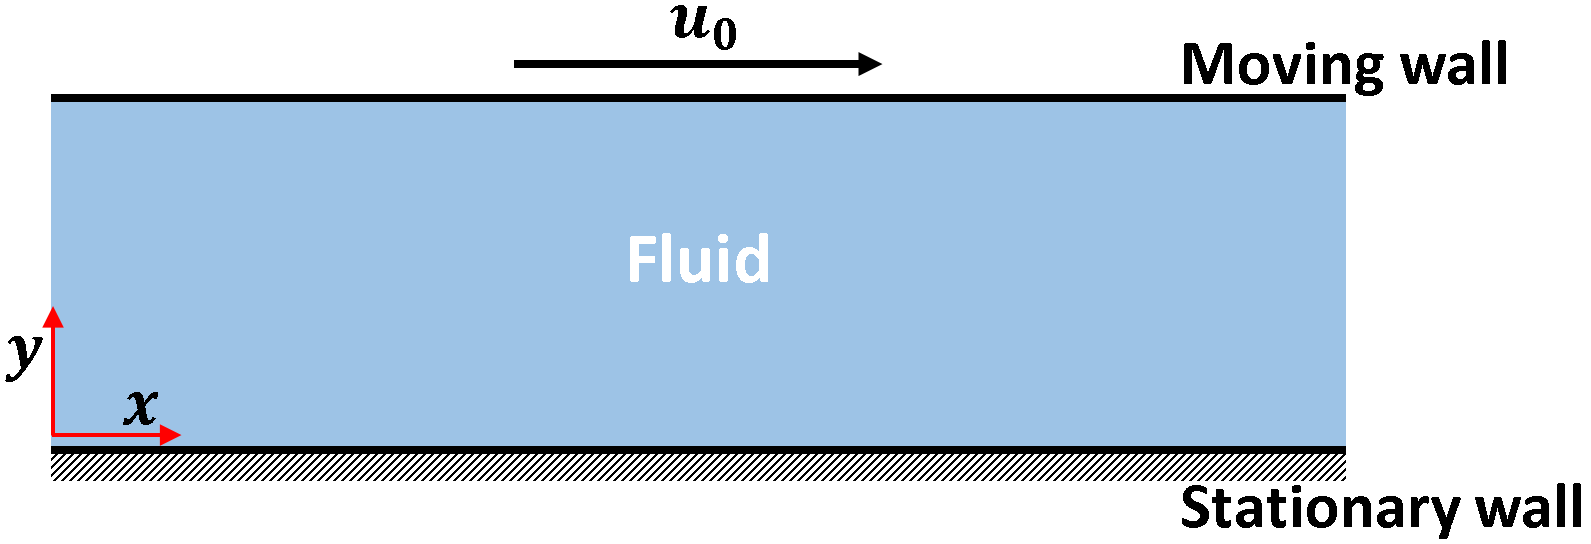
\includegraphics[width=14.00cm]{Chapter_3/figure/C3_infinite_channel.png}
	\caption{1D benchmark case for IB method.}
	\label{fig:C3_benchmarkCase}
\end{figure}

We can also assume that the boundary conditions are periodic in $x$. Next suppose that there is a horizontal plate running through the length of this channel at $y=y_0$ and moving with $u_0$ velocity in horizontal direction. We assume no-slip condition where the fluid and the plate meet. This will force the fluid to accelerate in $x$ direction due to the viscous stress from the moving plate. We expect no motion in $y$ direction and can drop all terms in the NS equations containing $u_j$ velocity. Due to the continuity equation \eqref{eq:C3_continuity}, there is no variation in the $x$ direction so we can drop all the terms that involve with $x$ variation as well. This enables us to simplify the NS equation of \eqref{eq:C3_momentum} into Equation \eqref{eq:C3_benchmarkProblem}. It should be noted that the continuum equation \eqref{eq:C3_continuity} is automatically satisfied.

\begin{subequations}\label{eq:C3_benchmarkProblem}
\begin{equation}
	u_t = \mu u_{yy} \quad \text{in } \Omega_f
\end{equation}
\begin{equation}
\begin{cases}
	u = u_0 \quad \text{at } y = 1 \\
	u = 0 \quad \text{at } y = 0
\end{cases}
\end{equation}
\end{subequations}

Equation \eqref{eq:C3_benchmarkProblem} is transient in nature however, its steady state solution can be calculated by setting the time derivative equal to zero. This equation governs what is commonly known as Couette flow in introductory courses in fluid dynamics. The analytical solution for this equation is shown in Equation \eqref{eq:C3_benchmarkAnalyticalSolution}.

\begin{equation}\label{eq:C3_benchmarkAnalyticalSolution}
	u = u_0 x
\end{equation}

We will use this analytical solution to verify the result of the different IB methods defined in the following sections.

% ======================================================================================
\section{Immersed Boundary Classification}
In general, IB methods can be classified in three main families: i) discrete forcing, ii) continuum forcing, and iii) cut-cell methods. This classification is based on how the interface conditions are handled in the IB algorithm. In this section we present the essence of each method and try to point their primary advantages and disadvantages. Moreover, each of the discussed IB techniques will be applied to the benchmark problem where the results are verified with the analytical solution. In general, the immersed boundary approach is based on modifying the NS equations for imposing the boundary conditions. This modification can be done in three different ways that leads to a fundamental dichotomy in IB method.

% ======================================================================================
\section{Discrete Forcing Method}
The discrete forcing approach was first introduced in the works of Mohd-Yusof \cite{mohd1997combined} in late nineties. The discrete forcing approach is defining the force in the numerical solution from the known characteristic of the repose. For the case of flow over immersed boundaries, this known characteristic is the flow velocity on the immersed boundary. The general formulation for the discrete forcing method starts with the discretized NS equation

\begin{equation}
	\frac{u^{n+1} - u^n}{\Delta t} = RHS^{n+1/2} + f^{n+1/2}
\end{equation}

where $u^{n+1}$ is the velocity at the next time step, $u^n$ is the velocity at the current time step, $\Delta t$ is the time step, and $RHS^{n+1/2}$ contains both the viscous terms and pressure gradient. $f^{n+1/2}$ is the forcing term that needs to be calculated in such a way that yields $u^{n+1} = V$, where $V$ is the known velocity of the immersed boundary. Therefore, the force term is calculated as

\begin{equation}
	f^{n+1/2} = -RHS^{n+1/2} + \frac{V - u^n}{\Delta t}
\end{equation}

This is valid only if the location of the immersed boundary coincides with the computational nodes. Interpolation from the fluid's computational nodes to the immersed boundary is needed for the cases where the two do not coincide. Depending on how this interpolation is done and where the force terms are calculated, the discrete forcing immersed boundary method is put into two main family based on this.

% -.-.-.-.-.-.-.-.-.-.-.-.-.-.-.-.-.-.-.-.-.-.-.-.-.-.-.-.-.-.-.-.-.-
\subsection{Direct forcing approach}


% -.-.-.-.-.-.-.-.-.-.-.-.-.-.-.-.-.-.-.-.-.-.-.-.-.-.-.-.-.-.-.-.-.-
\subsection{Ghost cell method}
In the ghost cell method, the conditions on the immersed boundary are imposed through a set of Ghost cells. These are the cells in the solid region that have at least one neighbour in the fluid domain. For example, the node $\phi$ in Figure \ref{fig:C3_ghostCell} is a ghost cell.

\begin{figure}[H]
	\centering
	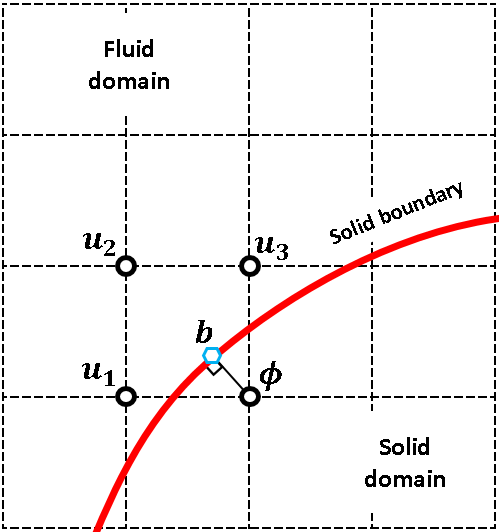
\includegraphics[width=7.00cm]{Chapter_3/figure/discrete_forcing_approach.png}
	\caption{Representation of nodes in the vicinity of an immersed boundary used in the ghost-cell approach.}
	\label{fig:C3_ghostCell}
\end{figure}

For each ghost cell, an interpolation is used to implicitly satisfy the desired value of response on the immersed boundary. The easiest interpolation used is the bilinear interpolation (trilinear in 3D) where the value of $\phi$ can be defined as

\begin{equation}
	\phi = C_1 x_1 x_2 + C_2 x_1 + C_3 x_2 + C_4
\end{equation}

where the four coefficients in above equation is calculated based on the values of flow response at $U_1$, $U_2$, $U_3$ from the solution and the known value at the boundary point $b$. Boundary point $b$, is the normal intercept from the ghost node to the immersed boundary. The linear interpolation is well suited for the laminar flows or for high Reynolds number flows where the gird points are located in the viscous sublayer \cite{iaccarino2003immersed}. For high Reynolds number where higher accuracy is required, higher-order interpolation are used. An example of such interpolations are suggested by Majumdat et al., where they employed a linear interpolation in the tangential direction and quadratic in the normal direction \cite{majumdar2001rans}. 

The ghost cell method, introduce the boundary conditions on the immersed boundary surface directly into the discrete equations. Therefore, the forcing term depends on the discretization process and its practical implementation is not straightforward compared to the continuous forcing approach which is discussed in the next section. The steps for implementing the ghost cell method can be summarized as follows

\begin{enumerate}
	\item Mark computational nodes as fluids, solids, and ghost cells based on their relative location to the boundary
	\item For each of ghost cells, define an interpolation scheme based on the neighbouring nodes
	\item Update the discretized equations for nodes with ghost cell in their boundaries using the interpolation scheme
	\item Solve the resulting equations for the response
	\item Update the interpolation scheme and discrete equations based on the new values
	\item loop until convergence is satisfied
\end{enumerate}

The ghost cell method is applied to the demonstration problem introduced in Section \ref{sec:C3_benchmark_case}. We chose linear interpolation for this problem since the velocities are rather small. looked at the effect of moving wall velocity and the number of nodes on the accuracy of the solution. The IB results are verified using the analytical solution of the problem. We derive the ghost cell method, by discretizing the domain using 6 nodes using central difference method. For demonstration we define the location of wall between nodes $2$ and $3$ as shown in Figure \ref{fig:C3_discretizedGhostCell}. This makes node $3$ the ghost cell for this problem.

\begin{figure}[H]
	\centering
	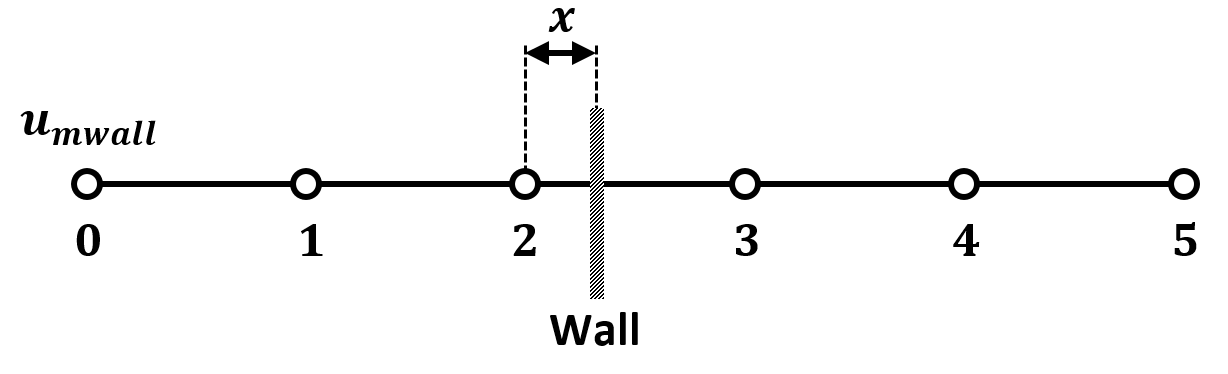
\includegraphics[width=10.00cm]{Chapter_3/figure/ghost_cell_discretization.png}
	\caption{Discretized domain for the ghost cell IB method where the \lq\lq wall\rq\rq\ is represented using hashed box.}
	\label{fig:C3_discretizedGhostCell}
\end{figure}

The solid wall is defined at location $x$ in the local coordinate of the space between nodes $2$ and $3$. By using this coordinate and linear interpolation between nodes $2$ and $3$, the response on the wall is defined as

\begin{equation}
	x u_3 + (1 - x) u_2 = u_{swall}
\end{equation}

where $u_i$ is response at node $i$ and $u_{swall}$ is the predefined velocity at the stationary wall. For this problem, we know that $u_{swall}$ is equal to zero. Therefore, the response at the ghost cell, $u_3$, needs to be equal to the following to ensure zero velocity on the fixed wall.

\begin{equation}\label{eq:C3_ghostCellValue}
	u_3 = -\frac{1 - x}{x} u_2
\end{equation}

The second-order central-difference differential operator for this problem is shown in Equation \eqref{eq:C3_centralDifferenceBefore}. By substituting Equation \eqref{eq:C3_ghostCellValue} in Equation \eqref{eq:C3_centralDifferenceBefore}, we modify the differential operator in a way that it incorporates the effect of solid boundary. This modified operator is shown in Equation \eqref{eq:C3_centralDifferenceAfter}. It should be noted that since the value of $u_3$ is known from Equation \eqref{eq:C3_ghostCellValue}, its corresponding equation is remove from Equation \eqref{eq:C3_centralDifferenceBefore}.

\begin{subequations}
\begin{equation}\label{eq:C3_centralDifferenceBefore}
	L = 
	\begin{bmatrix}
	1 & -2 & 1 & 0 & 0 & 0 \\
	0 & 1 & -2 & 1 & 0 & 0 \\
	0 & 0 & 1 & -2 & 1 & 0 \\
	0 & 0 & 0 & 1 & -2 & 1
	\end{bmatrix} \quad \text{:original operator}
\end{equation}
\begin{equation}\label{eq:C3_centralDifferenceAfter}
	L' = 
	\begin{bmatrix}
	1 & -2 & 1 & 0 & 0 & 0 \\
	0 & 1 & -2-(1-x)/x & 0 & 0 & 0 \\
	0 & 0 & 1+2(1-x)/x & 0 & 1 & 0 \\
	0 & 0 & -(1-x)/x & 0 & -2 & 1
	\end{bmatrix} \quad \text{:modified operator}
\end{equation}
\end{subequations}

The differential operator of Equation \eqref{eq:C3_centralDifferenceAfter} needs to be updated based on the new location of wall. This may cause a different column to become zero. As a results, we need to know the discretization technique used in solving the governing equations in order to implement the ghost method method. This is not usually possible for the commercial packages.

The Euler method is used for time integration of the discrete equations. In the discrete form, this is written as shown in Equation \eqref{eq:C3_euelrMethodBefore}. The time integration is also need to be modified to incorporate the effect of the ghost cell. This is done by incorporating the known value of ghost cell in the time integration as shown in Equation \eqref{eq:C3_euelrMethodAfter}.

\begin{subequations}
\begin{equation}\label{eq:C3_euelrMethodBefore}
	\begin{bmatrix}
	1 & 0 & 0 & 0 \\
	0 & 1 & 0 & 0 \\
	0 & 0 & 1 & 0 \\
	0 & 0 & 0 & 1
	\end{bmatrix}
	\begin{bmatrix}
	u_1^{n+1} \\
	u_2^{n+1} \\
	u_3^{n+1} \\
	u_4^{n+1}
	\end{bmatrix}
	=
	\begin{bmatrix}
	1 & 0 & 0 & 0 \\
	0 & 1 & 0 & 0 \\
	0 & 0 & 1 & 0 \\
	0 & 0 & 0 & 1
	\end{bmatrix}
	\begin{bmatrix}
	u_1^{n} \\
	u_2^{n} \\
	u_3^{n} \\
	u_4^{n}
	\end{bmatrix}
	+ 
	\Delta t L \mathbf{u}^n
\end{equation}
\begin{equation}\label{eq:C3_euelrMethodAfter}
	\begin{bmatrix}
	1 & 0 & 0 & 0 \\
	0 & 1 & 0 & 0 \\
	0 & 0 & 1 & 0 \\
	0 & 0 & 0 & 1
	\end{bmatrix}
	\begin{bmatrix}
	u_1^{n+1} \\
	u_2^{n+1} \\
	u_3^{n+1} \\
	u_4^{n+1}
	\end{bmatrix}
	=
	\begin{bmatrix}
	1 & 0 & 0 & 0 \\
	0 & 1 & 0 & 0 \\
	0 & -(1-x)/x & 0 & 0 \\
	0 & 0 & 0 & 1
	\end{bmatrix}
	\begin{bmatrix}
	u_1^{n} \\
	u_2^{n} \\
	u_3^{n} \\
	u_4^{n}
	\end{bmatrix}
	+ 
	\Delta t L' \mathbf{u}^n
\end{equation}
\end{subequations}

where $L'$ is the modified differential operator of Equation \eqref{eq:C3_centralDifferenceAfter}. It is clear that excessive modification of the discrete solver is required for implementation of the immersed boundary. This discretization method is applied to the benchmark case, we the effect of node number, location of the stationary wall, and the wall velocity on the solution accuracy is investigated.
% ======================================================================================
\section{Continuum Forcing Method}
In this implementation of the immersed boundary, a forcing equation is added to the continuous governing equation \eqref{eq:C3_momentum} to represent the effect of the boundary. The continuous IB technique is the original method developed by Peskin \cite{peskin1972flow} for coupled simulation of blood flow due to the contraction of heart muscle. In this approach, the immersed boundary is represented by a set of elastic fibers that their locations are tracked in a Lagrangian fashion by a collection of massless points. These points move with the local fluid velocity. Therefore, the location of the $k$-th Lagrangian point, $X_k$ is governed by the following equation

\begin{equation}
	\frac{\partial X_k}{\partial t} = u(X_k, t)
\end{equation}

where $u$ is the velocity of the fluid at location $X_k$. The location of fluid nodes, $x$, does not necessary coincide with the location of the Lagrangian points. Thus, it is required to map the velocities from the Eulerian domain, where the fluid's equation of motion are solved, to Lagrangian nodes. In a purely continuum problem, this can be done using the Dirac delta functions. The property of the Dirac delta function that enables the mapping between the Euler and Lagrangian domain is shown in the following equation

\begin{equation}
	\int_{\Omega_f} f(x) \delta(x - X_k) = f(X_k)
\end{equation}

As can be seen here, by convoluting the function of interest and the delta function, we can evaluate our function of interest at any location where the delta function is defined. By defining the delta function at $X_k$ and using velocity from CFD solver as function $f$, we can evaluate the needed velocity for IB at any arbitrary point $X_k$. Although this is the main idea of mapping data to Lagrangian domain, this approach becomes unstable in practice \cite{lee2003stability}. In the practical implementation of immersed boundary method, the effect of delta function need to be expanded to couple of nodes around $X_k$. This is achieved by relaxing the delta function. The relaxed delta function is generally refereed to as regularized delta function \cite{shin2008assessment}. The regularized delta function is defined using Equation \eqref{eq:C3_regularizedDeltaFunction} in three dimensions.

\begin{equation}\label{eq:C3_regularizedDeltaFunction}
	\delta_h(x_1, x_2, x_3) = \frac{1}{dx_1 \cdot dx_2 \cdot dx_3}
							   \phi \left( \frac{x_1 - \eta_1}{dx_1} \right)
							   \phi \left( \frac{x_2 - \eta_2}{dx_2} \right)
							   \phi \left( \frac{x_2 - \eta_3}{dx_3} \right)
\end{equation}

where $x_i$ is the spatial coordinate in each direction, $\eta_i$ is the location where the delta function is defined, and $dx_i$ is the grid size in each direction. In above equation $i$ can be $1$, $2$, or $3$. The $\phi$ function is defined in Equation \eqref{eq:C3_phiFunction}. As shown here there are different ways of defining this function. The input of $\phi$ function is $r$ which is defined as $(x_i - \eta_i) / dx_i$.

\begin{subequations}\label{eq:C3_phiFunction}
\begin{equation}\label{eq:C3_phiFunction_2point}
	\phi(r) = 
	\begin{cases}
	1 - |r| \quad &|r| \leq 1 \\
	0	\quad &\text{otherwise}
	\end{cases}
\end{equation}
\begin{equation}\label{eq:C3_phiFunction_3point}
	\phi(r) = 
	\begin{cases}
		\frac{1}{3} \left( 1 + \sqrt{-3r^2 + 1} \right) \quad &|r| \leq 0.5 \\
		\frac{1}{6} \left( 5 - 3|r| - \sqrt{-3(1 - |r|)^2 + 1} \right) & 0.5 \geq |r| \leq 1.5 \\
		0 & \text{otherwise}
	\end{cases}
\end{equation}
\begin{equation}\label{eq:C3_phiFunction_4point}
	\phi(r) = 
	\begin{cases}
		\frac{1}{8}
		\left(
		3 - 2|r| + \sqrt{1 + 4|r| - 4r^2}
		\right) \quad &0 \leq |r| \leq 1
		\\
		\frac{1}{8}
		\left(
		5 - 2|r| + \sqrt{-7 + 12|r| - 4r^2}
		\right) \quad &1 \leq |r| \leq 2
		\\
		0 &\text{otherwise}
	\end{cases}
\end{equation}
\begin{equation}\label{eq:C3_phiFunction_6point}
	\phi(r) = 
	\begin{cases}
		\begin{split}
		\frac{61}{112} - \frac{11}{42} |r| - \frac{11}{56} |r|^2 + \frac{1}{12} |r|^3 + 
		\frac{\sqrt{3}}{336}
		\left( 243 + 1584 |r| \right. \\
		\left. - 748 |r|^2 - 1560 |r|^3 + 500 |r|^4 + 336 |r|^5 - 112 |r|^6
		\right)^{1/2}
		\end{split} \quad & 0 \leq |r| \leq 1
		\\
		\frac{21}{16} + \frac{7}{12} |r| - \frac{7}{8} |r|^2 + \frac{1}{6} |r|^3 - 
		\frac{3}{2} \phi \left( |r| - 1 \right) & 1 \leq |r| \leq 2
		\\
		\frac{9}{8} - \frac{23}{12} |r| + \frac{3}{4} |r|^2 - \frac{1}{12} |r|^3 + 
		\frac{1}{2} \phi \left( |r| - 2 \right) & 2 \leq |r| \leq 3
		\\
		0 & \text{otherwise}
	\end{cases}
\end{equation}
\end{subequations}

Equation \eqref{eq:C3_phiFunction_2point} is the 2-point delta function that does the linear interpolation between the points point \cite{saiki1996numerical}. Equation \eqref{eq:C3_phiFunction_3point} shoes the 3-point delta function used by Roma et al. \cite{roma1999adaptive}, and Equation \eqref{eq:C3_phiFunction_4point} and \eqref{eq:C3_phiFunction_6point} are 4-point and 6-point delta functions used by Peskin \cite{peskin2002immersed}. The comparison between the shape of different $\phi(r)$ functions are shown in Figure \ref{fig:C3_phi_function}

\begin{figure}
	\centering
	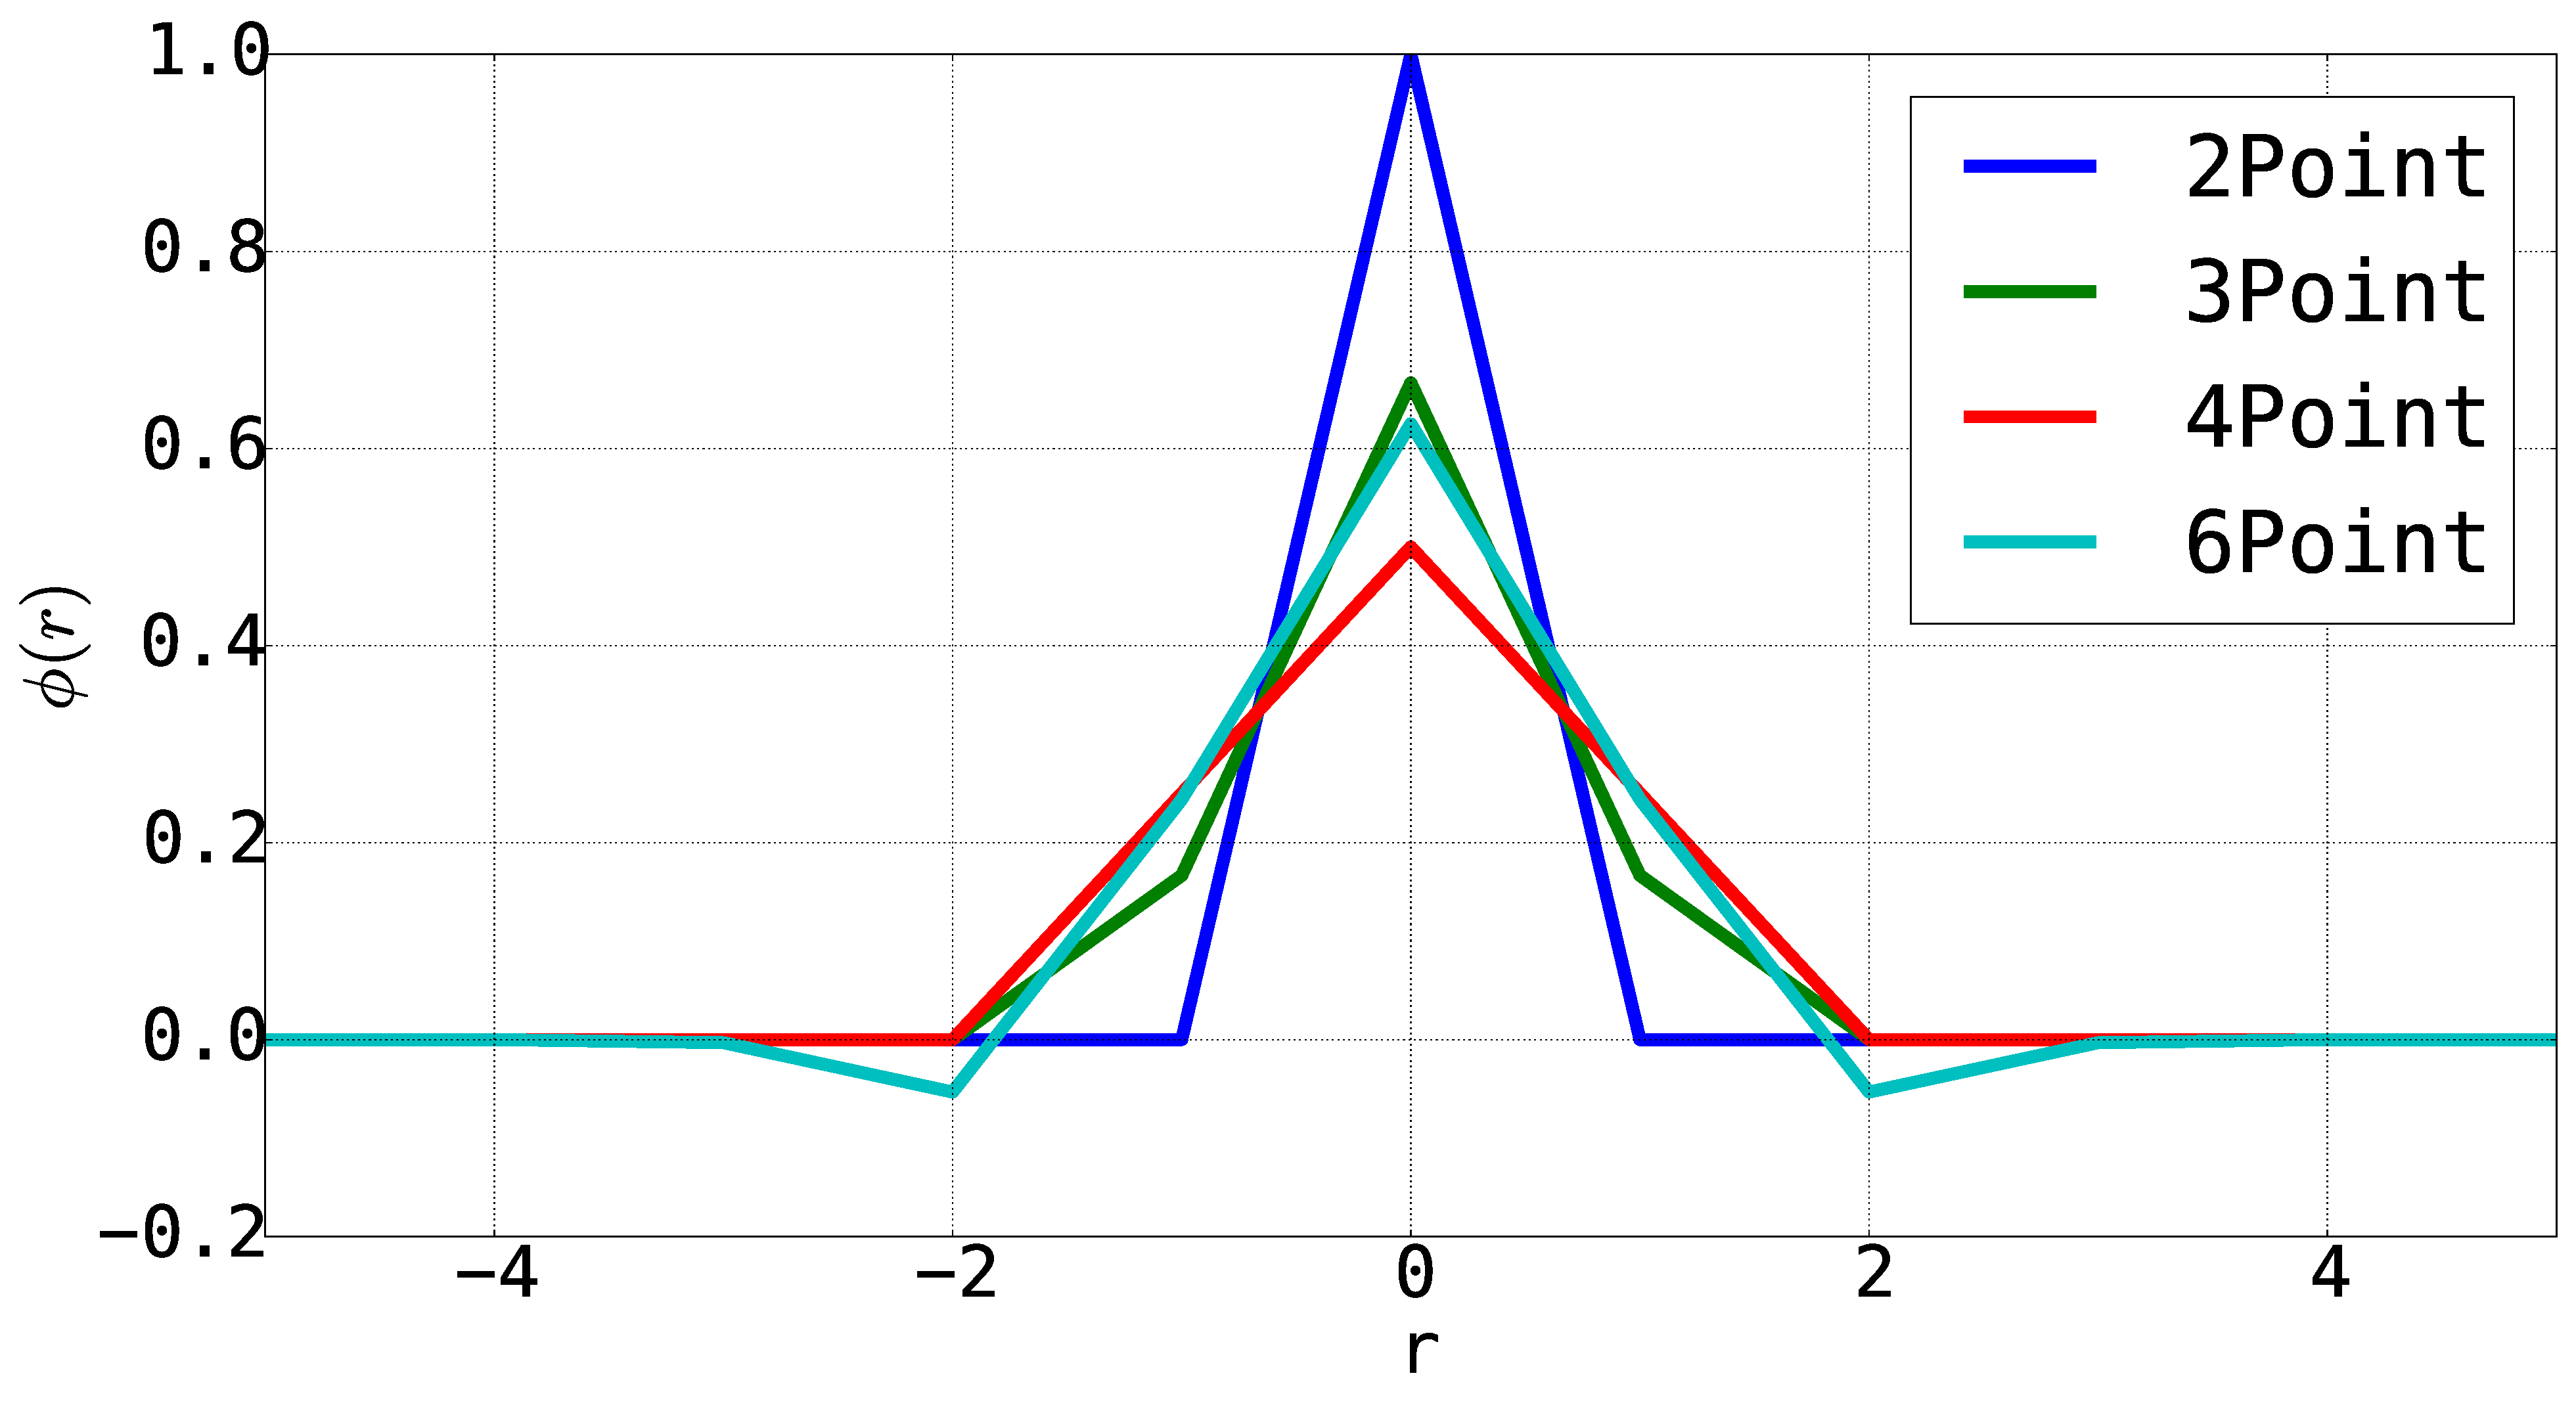
\includegraphics[width=14.cm]{Chapter_3/figure/phi_function.eps}
	\caption{Comparison between different formulations for $\phi$}
\end{figure}

Now we can write the mapping from the Eulerian nodes of the fluid solver to Lagrangian nodes as shown in Equation \eqref{eq:C3_lagrange2euler}.

\begin{equation}\label{eq:C3_lagrange2euler}
	u(X_k) = \int_\Omega u(x) \delta(x - X_k) dx
\end{equation}

where $\Omega$ is the computational domain, $u(x)$ is the velocity at the Eulerian nodes, $x$ is the coordinate of the Eulerian nodes, $u(X_k)$ is the velocity at the desired Lagrangian node, and $X_k$ is the coordinate of the Lagrangian node. Most of the continuum forcing approaches are the same upto this point. They diverge depending of the way they calculate the forcing terms.

% -.-.-.-.-.-.-.-.-.-.-.-.-.-.-.-.-.-.-.-.-.-.-.-.-.-.-.-.-.-.-.-.-.-Classical IB method
\subsection{Classical IB method}
In the classical IB method, the forces at the immersed boundaries are calculate using appropriate constitutive laws, i.e. Hooks law. This can be expressed as follows.

\begin{equation}
	f(X_k) = \mathcal{M}(X_k)
\end{equation}

where $\mathcal{M}$ is an operator which describes the properties of the boundaries. This force is calculated at the Lagrangian points and need to be transferred back to the Eulerian nodes. This is done using the same delta functions used previously to map the Eulerian results to Lagrangian. This method is well suited for a case of elastic bodies but will break for the cases of rigid boundaries or when the rigidity of boundaries are much more than the fluid. The origin of this problem is due to the high cycle oscillations that occur near the boundaries.

This approach is applied to the demonstration problem defined in Section \ref{sec:C3_benchmark_case}. We modelled the location of the fixed boundary using the classical IB method and verified the results using analytical formulas for this problem. The forcing function is added to the right-hand-side of the governing equation as follows

\begin{equation}
	\frac{\partial u}{\partial t} = \frac{\partial^2 u}{\partial y^2} - f(t)
\end{equation}

where $f(t)$ is the forcing function using to model the boundary. This equation is discretized using the Cranck-Nicholson method as follows

\begin{equation}\label{eq:C3_discretizedEquationPeskinIB}
	u^{n+1} = u^{n} + \frac{\Delta t}{2} \left( \frac{\partial^2 u^{n+1}}{\partial x^2} + 
	                                            \frac{\partial^2 u^n}{\partial x^2}\right) - \Delta t f^n 
\end{equation}

The steps to solve this equation and model the stationary wall using the IB method are as follows

\begin{enumerate}
	\item Define the initial condition as $u^0$ and set $f^0$ equal to zero.
	\item Calculate the velocity at the next time step, $u^1$, using Equation \eqref{eq:C3_discretizedEquationPeskinIB}
	\item Based on the new velocity at $t=1$ calculate the velocity at the location where the stationary wall is supposed to be, $X$, using $\delta$ function ($U$).
	\item Calculate the distance that this node will move in the current time step: $X^{n+1} = X^n + U \Delta t$
	\item Based on the new location of the node, calculate the forces as: $F = K \left( X^{n+1} - X^0 \right)$, where $X^0$ is the desired location of the wall and $K$ is the stiffness of wall. 
	\item Map the force at the Lagrangian location $X$ to its neighbouring Eulerian points using $\delta$ function.
	\item Reiterate until the convergence is satisfied.
\end{enumerate}

For the classical IB method, we investigated the accuracy of the results to the number of nodes, wall velocity, and the stiffness used to model the wall. The immersed boundary simulation is compared with analytical solution of this problem. We chose the normalized root mean square error to compared the analytical and IB results. This is defined as follows.

\begin{equation*}
	NRMSE = \dfrac{\sqrt{\dfrac{\sum_{n=1}{N} \left( \hat{y}_n - y \right)^2}{n}}}{y_{max} - y_{min}}
\end{equation*}

where $\hat{y}_t$ is the predicted value, $y$ is the true value, and $n$ is the number data points. Normalizing by $y_{max} - y_{min}$ enables us to compare models with different scales. This is especially useful when compared the results for different wall velocities.

For the first investigation, we selected the wall stiffness as $10^2$ and its location is selected as $x_{wall} = 0.51885$. We chose this location so that it does not coincide with the location of computational nodes. The time step is chosen as $10^{-5}$ and the wall velocity is fixed at $1 m/s$. For this simulation we used both 2-point and 4-point delta functions to transfer results between Lagrangian and Eulerian nodes. The computation domain is discretized using $11$, $41$, $81$, and $161$ nodes. The results of IB method is verified with analytical results.

\begin{figure}[H]
	\centering
	\subfigure[N = 11, 2-point delta function]
	{
	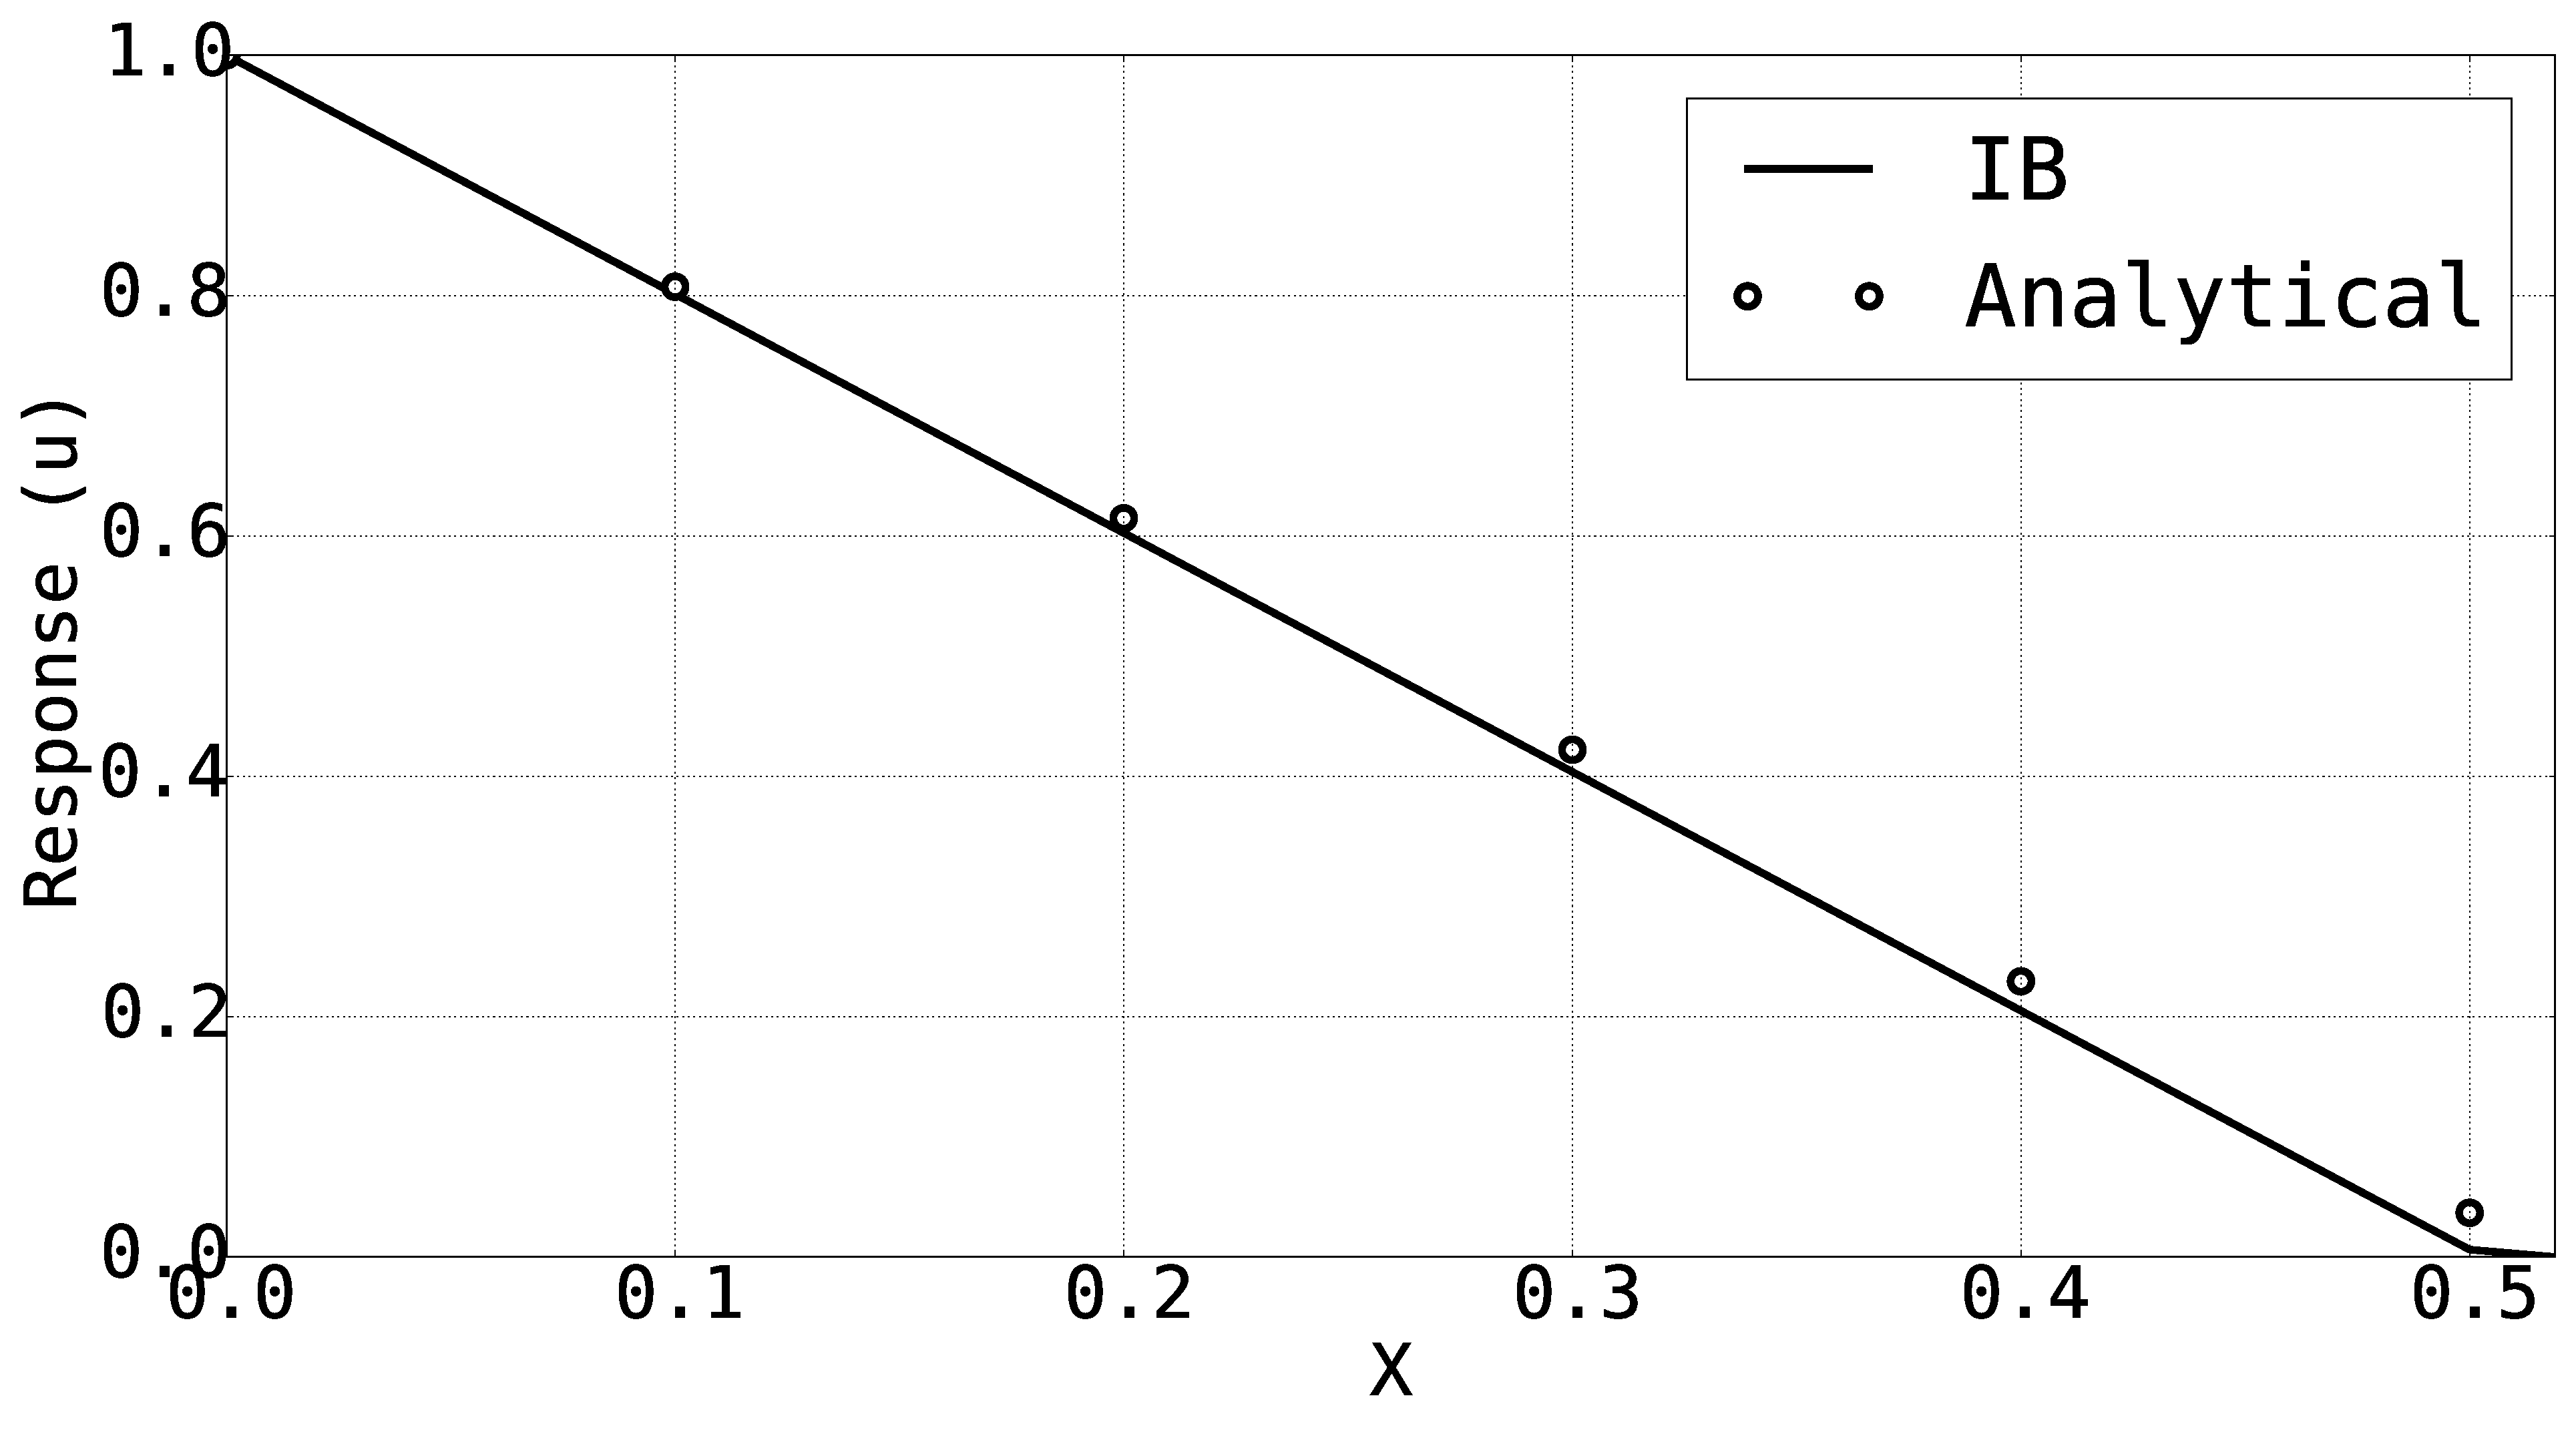
\includegraphics[width=7.0cm]{Chapter_3/figure/classicalIB_nodeNumber_2point_11.eps}
	}
	\quad
	\subfigure[N = 11, 4-point delta function]
	{
	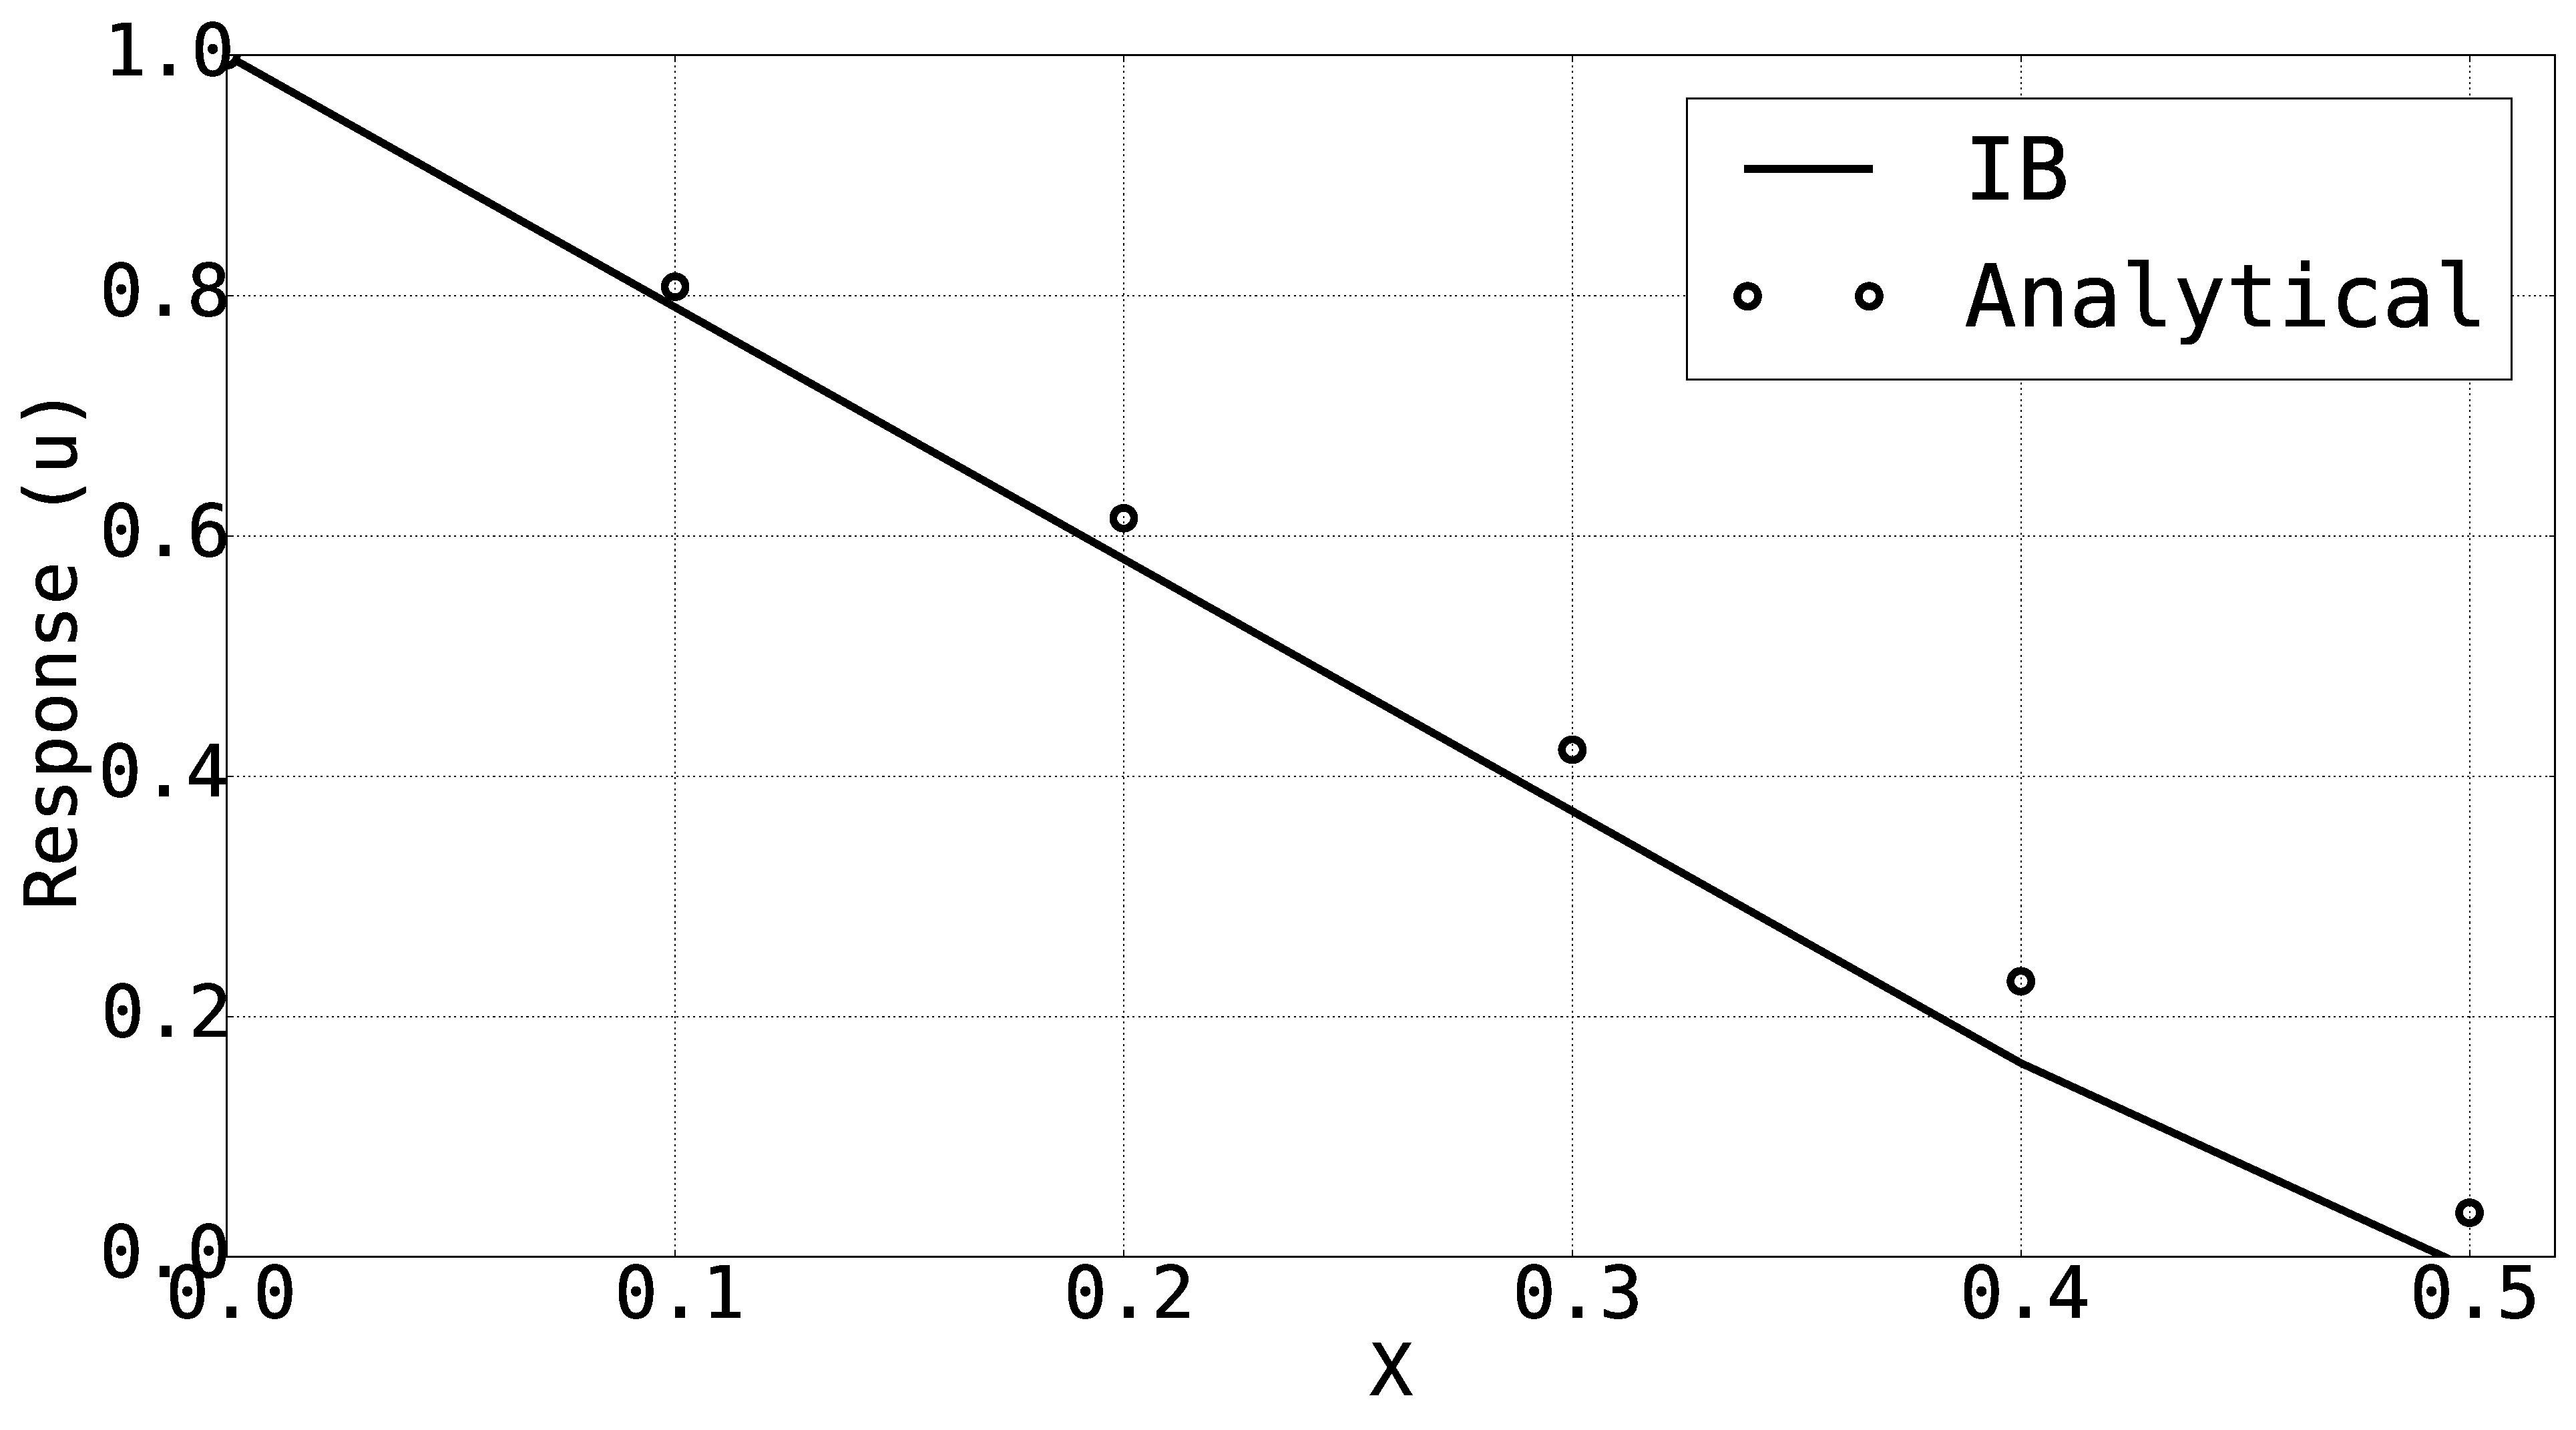
\includegraphics[width=7.0cm]{Chapter_3/figure/classicalIB_nodeNumber_4point_11.eps}
	}
	\\
	\subfigure[N = 41, 2-point delta function]
	{
	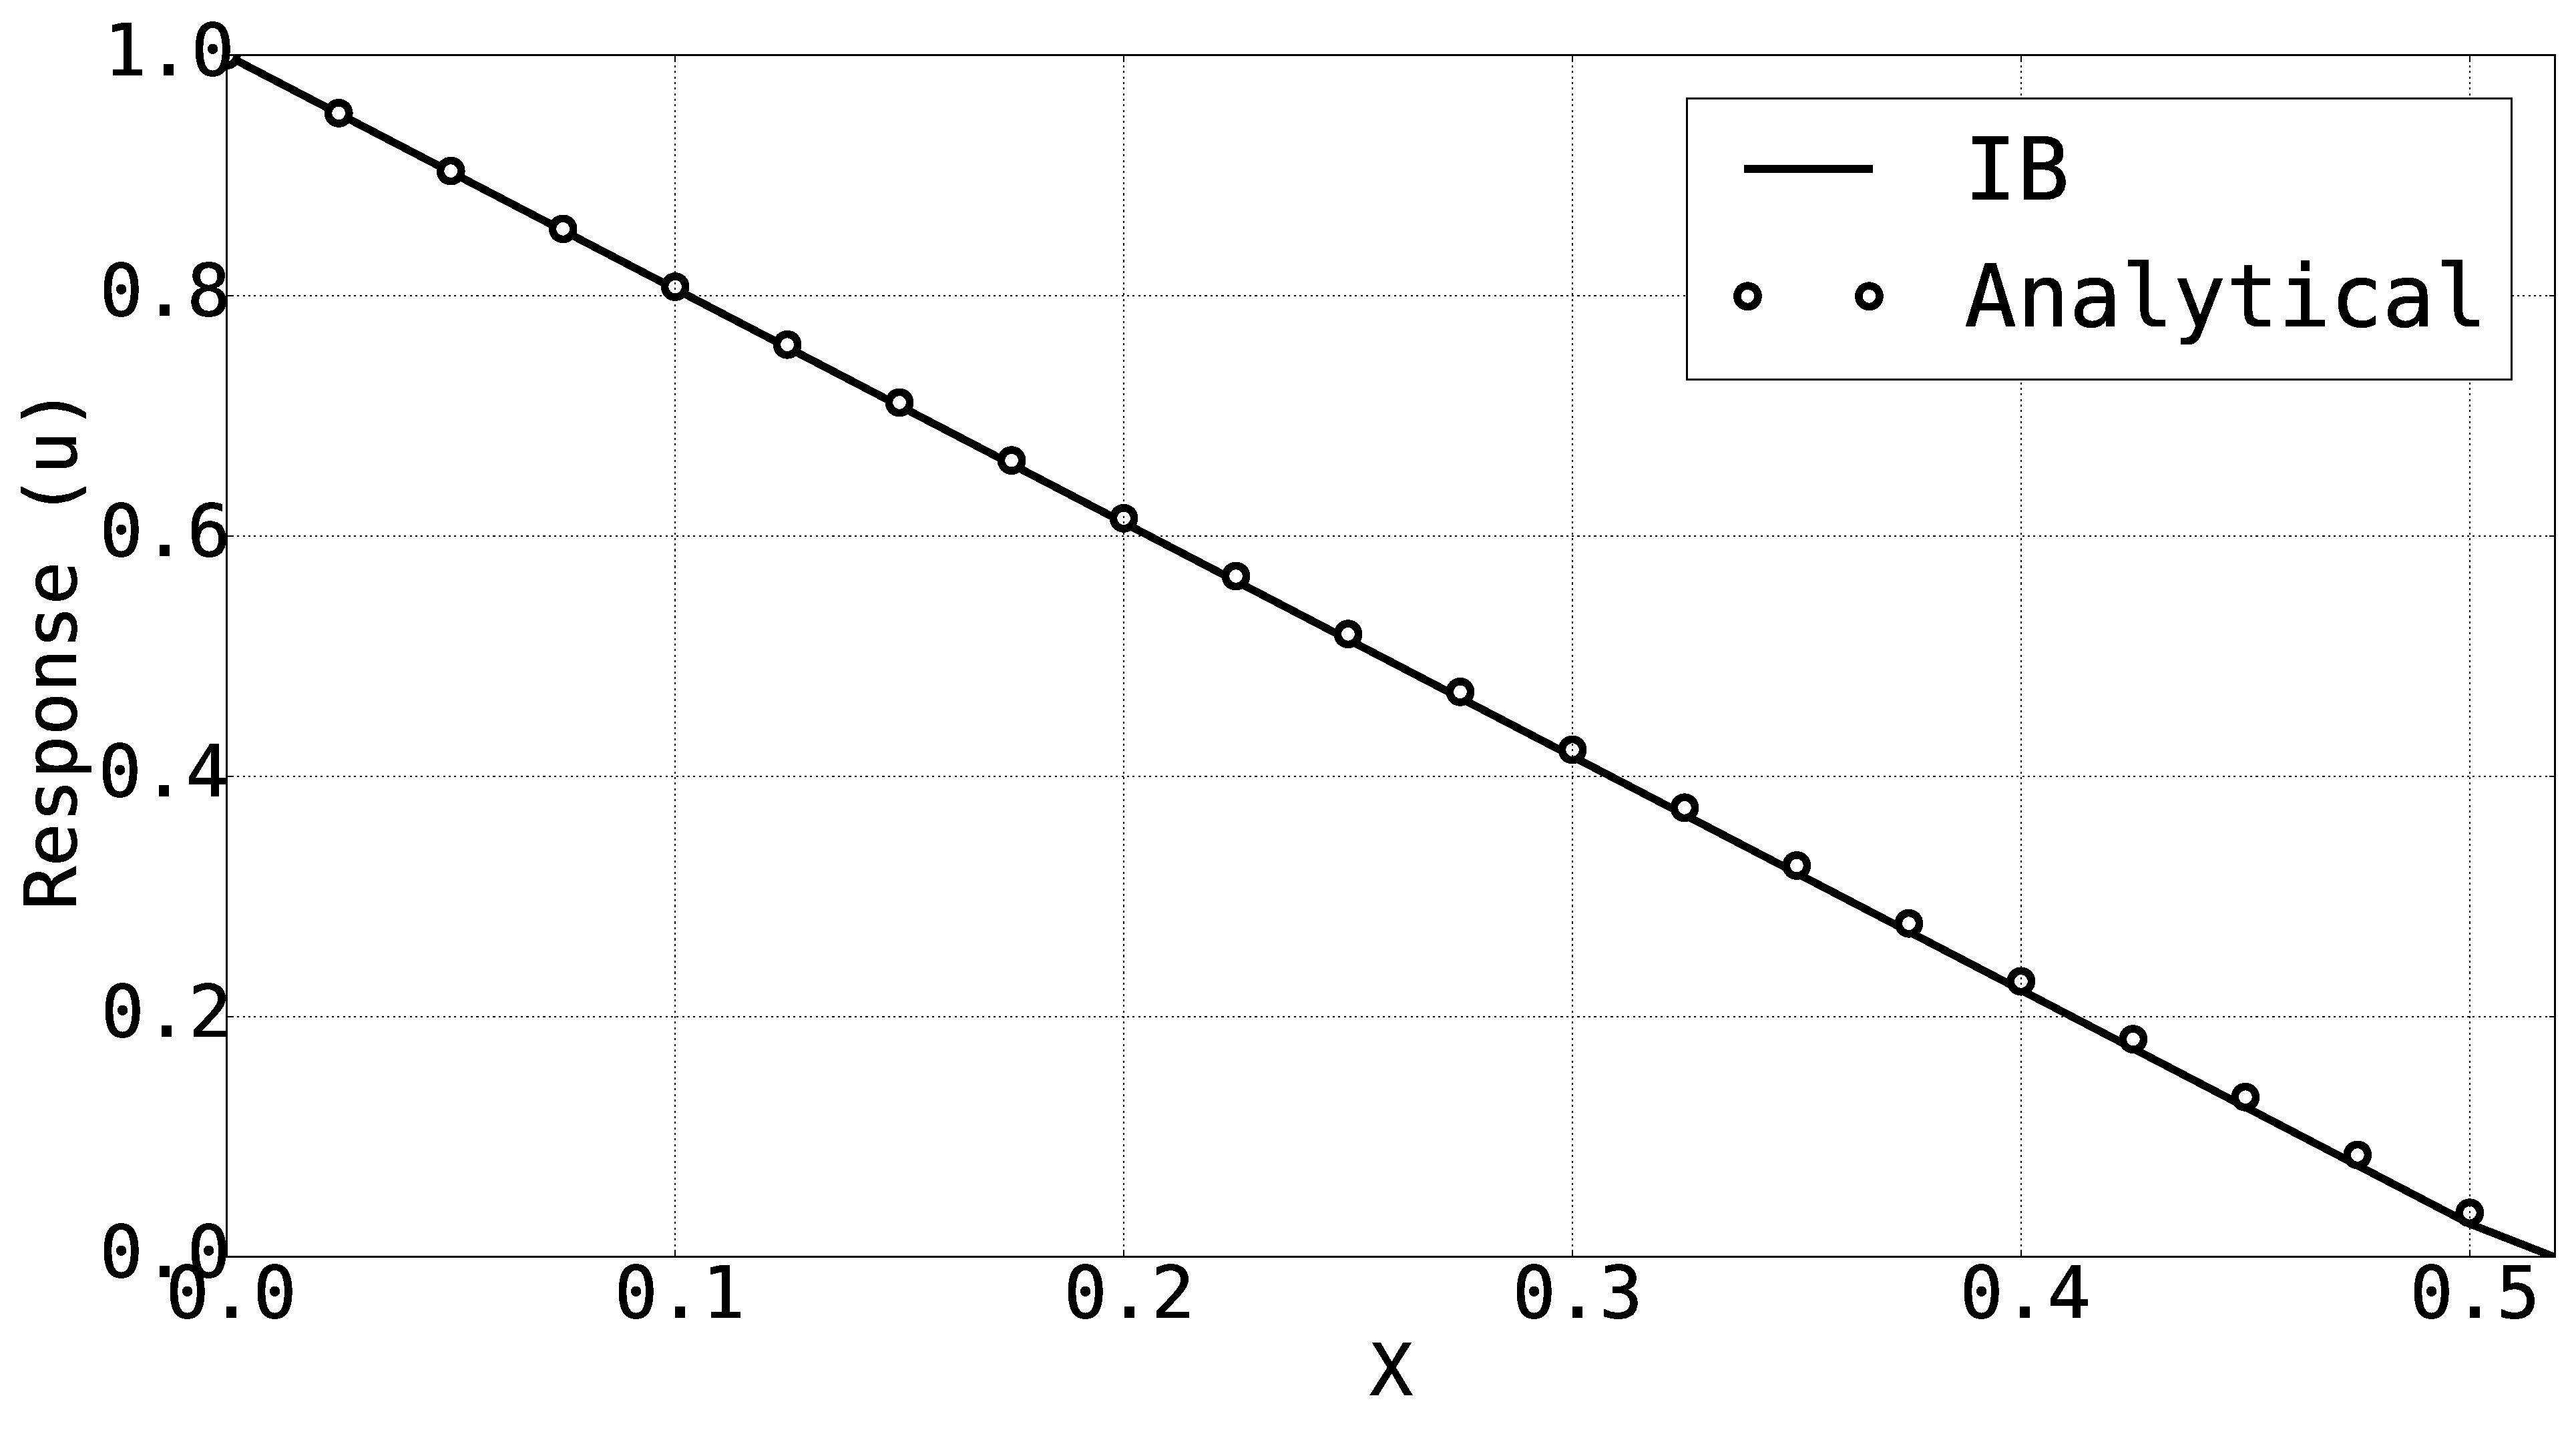
\includegraphics[width=7.0cm]{Chapter_3/figure/classicalIB_nodeNumber_2point_41.eps}
	}
	\quad
	\subfigure[N = 41, 4-point delta function]
	{
	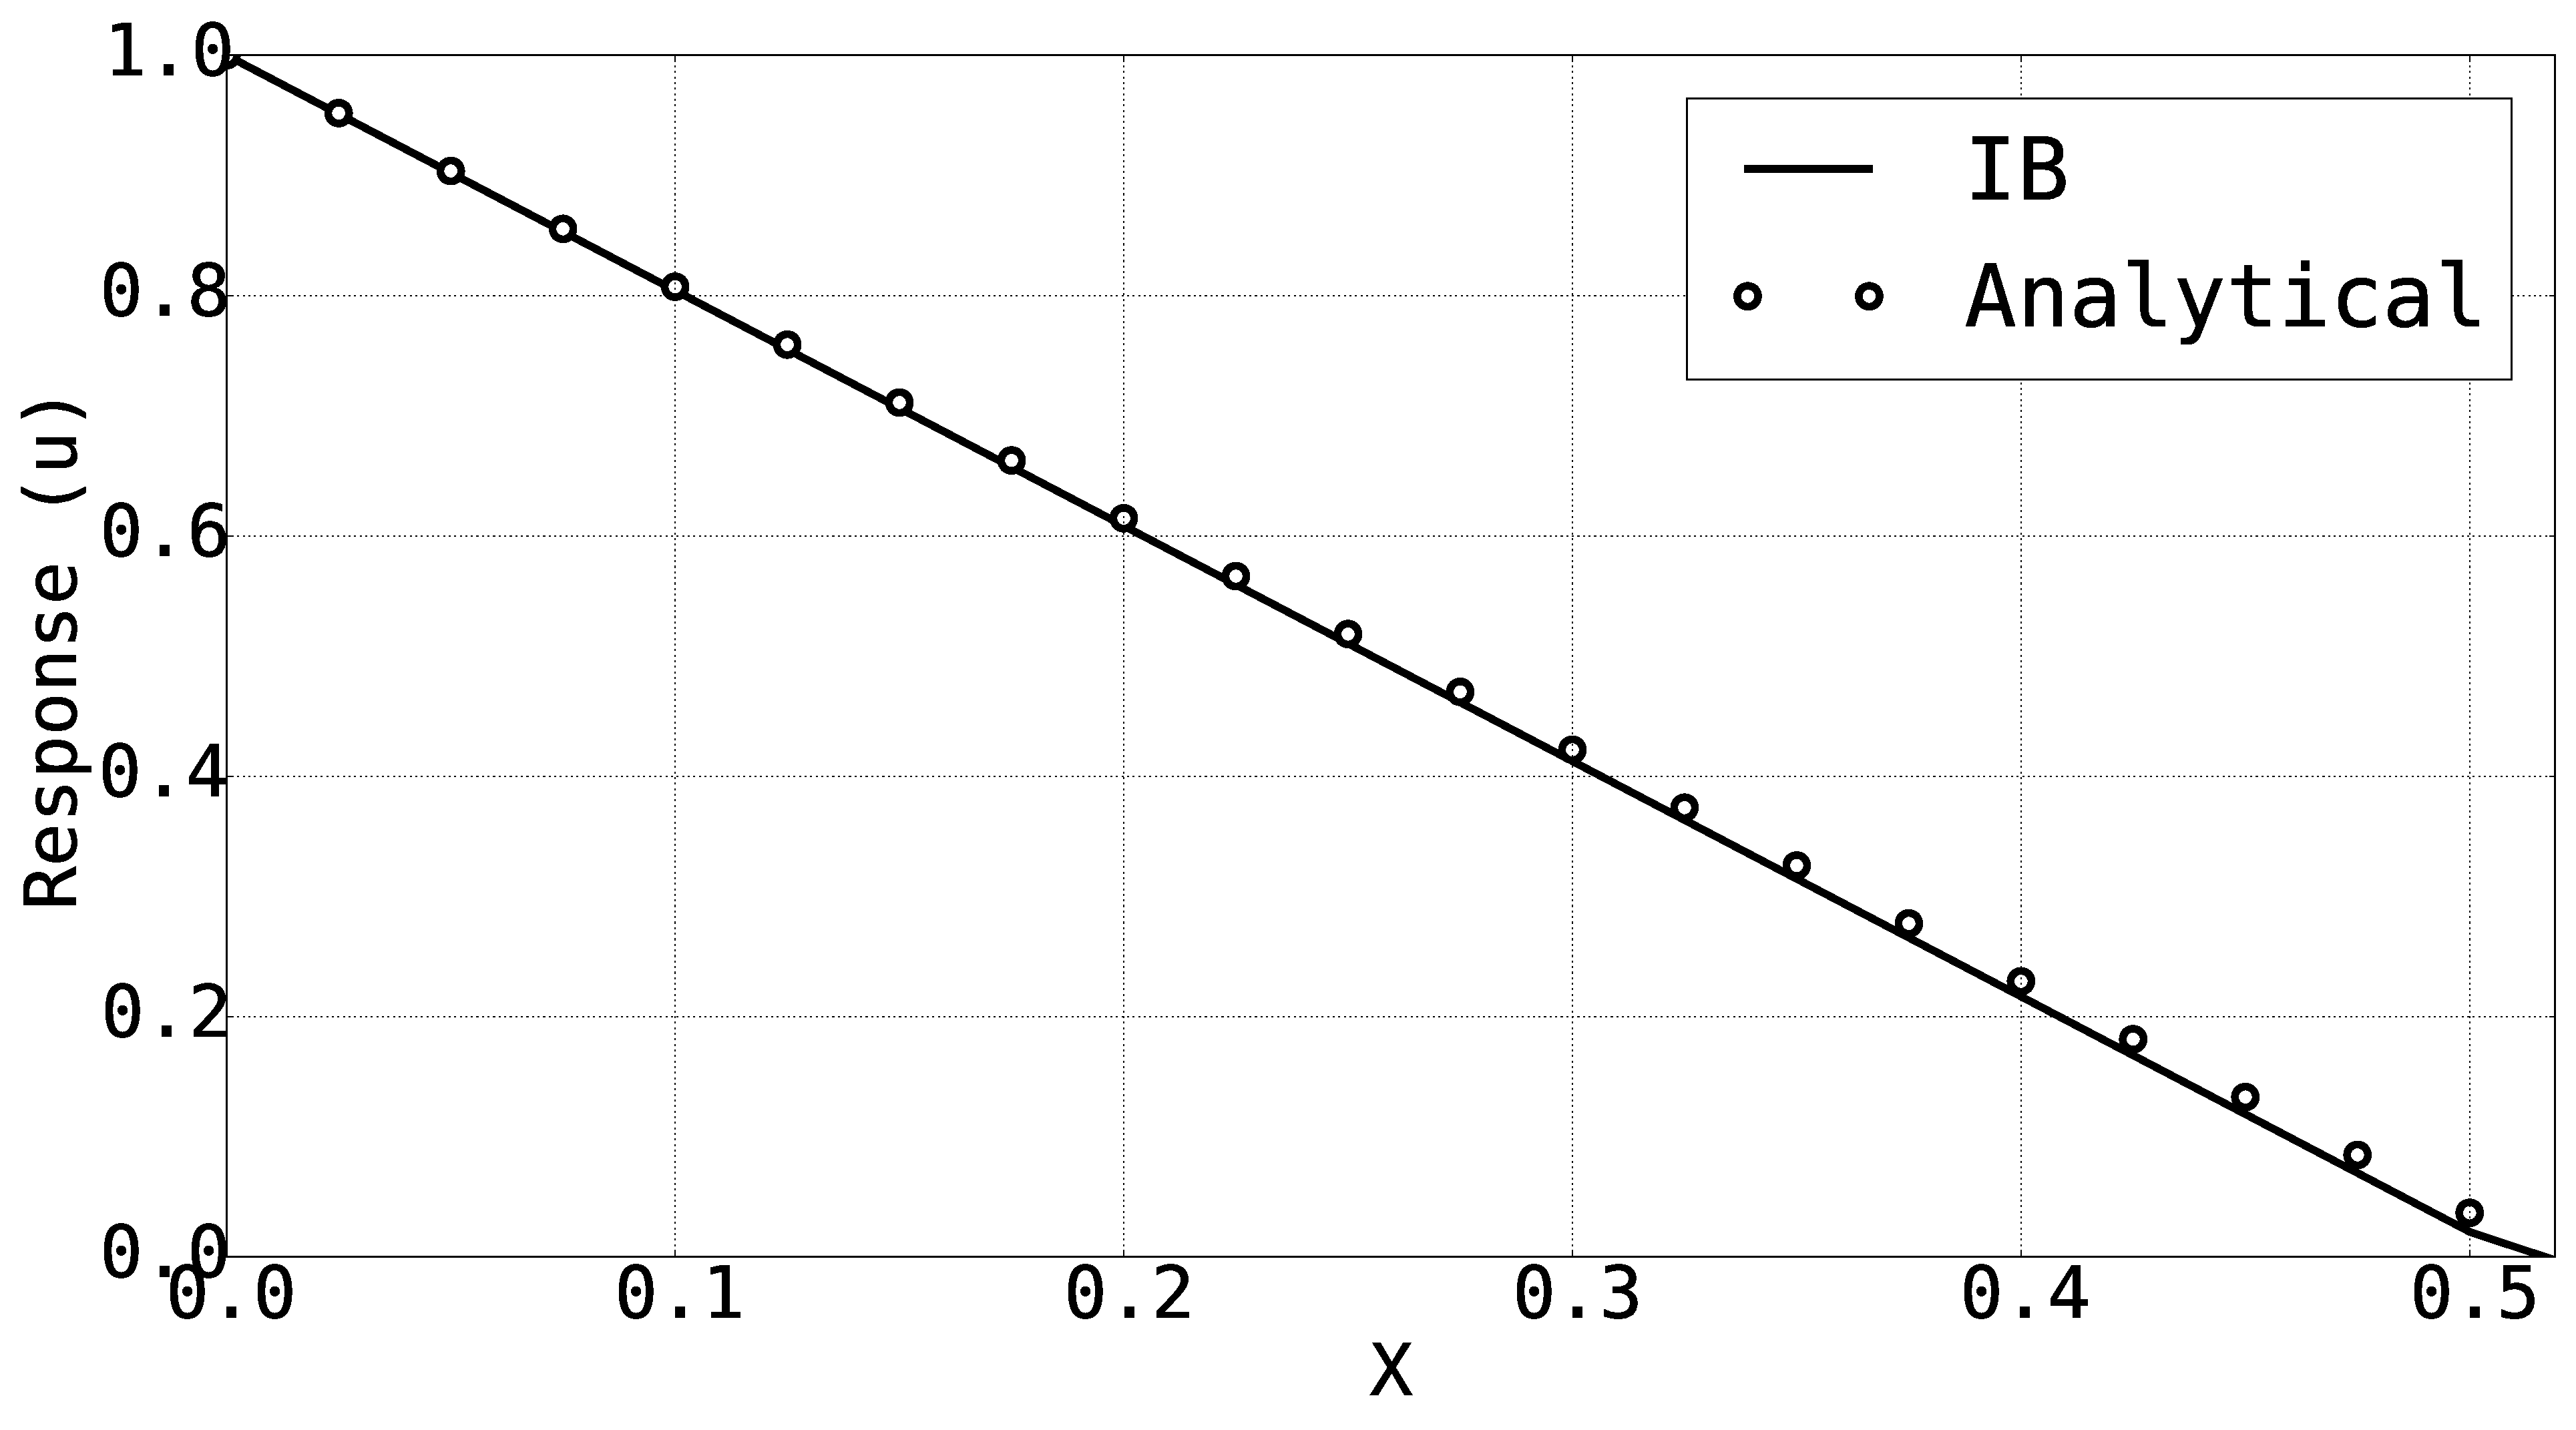
\includegraphics[width=7.0cm]{Chapter_3/figure/classicalIB_nodeNumber_4point_41.eps}
	}
	\\
	\subfigure[N = 81, 2-point delta function]
	{
	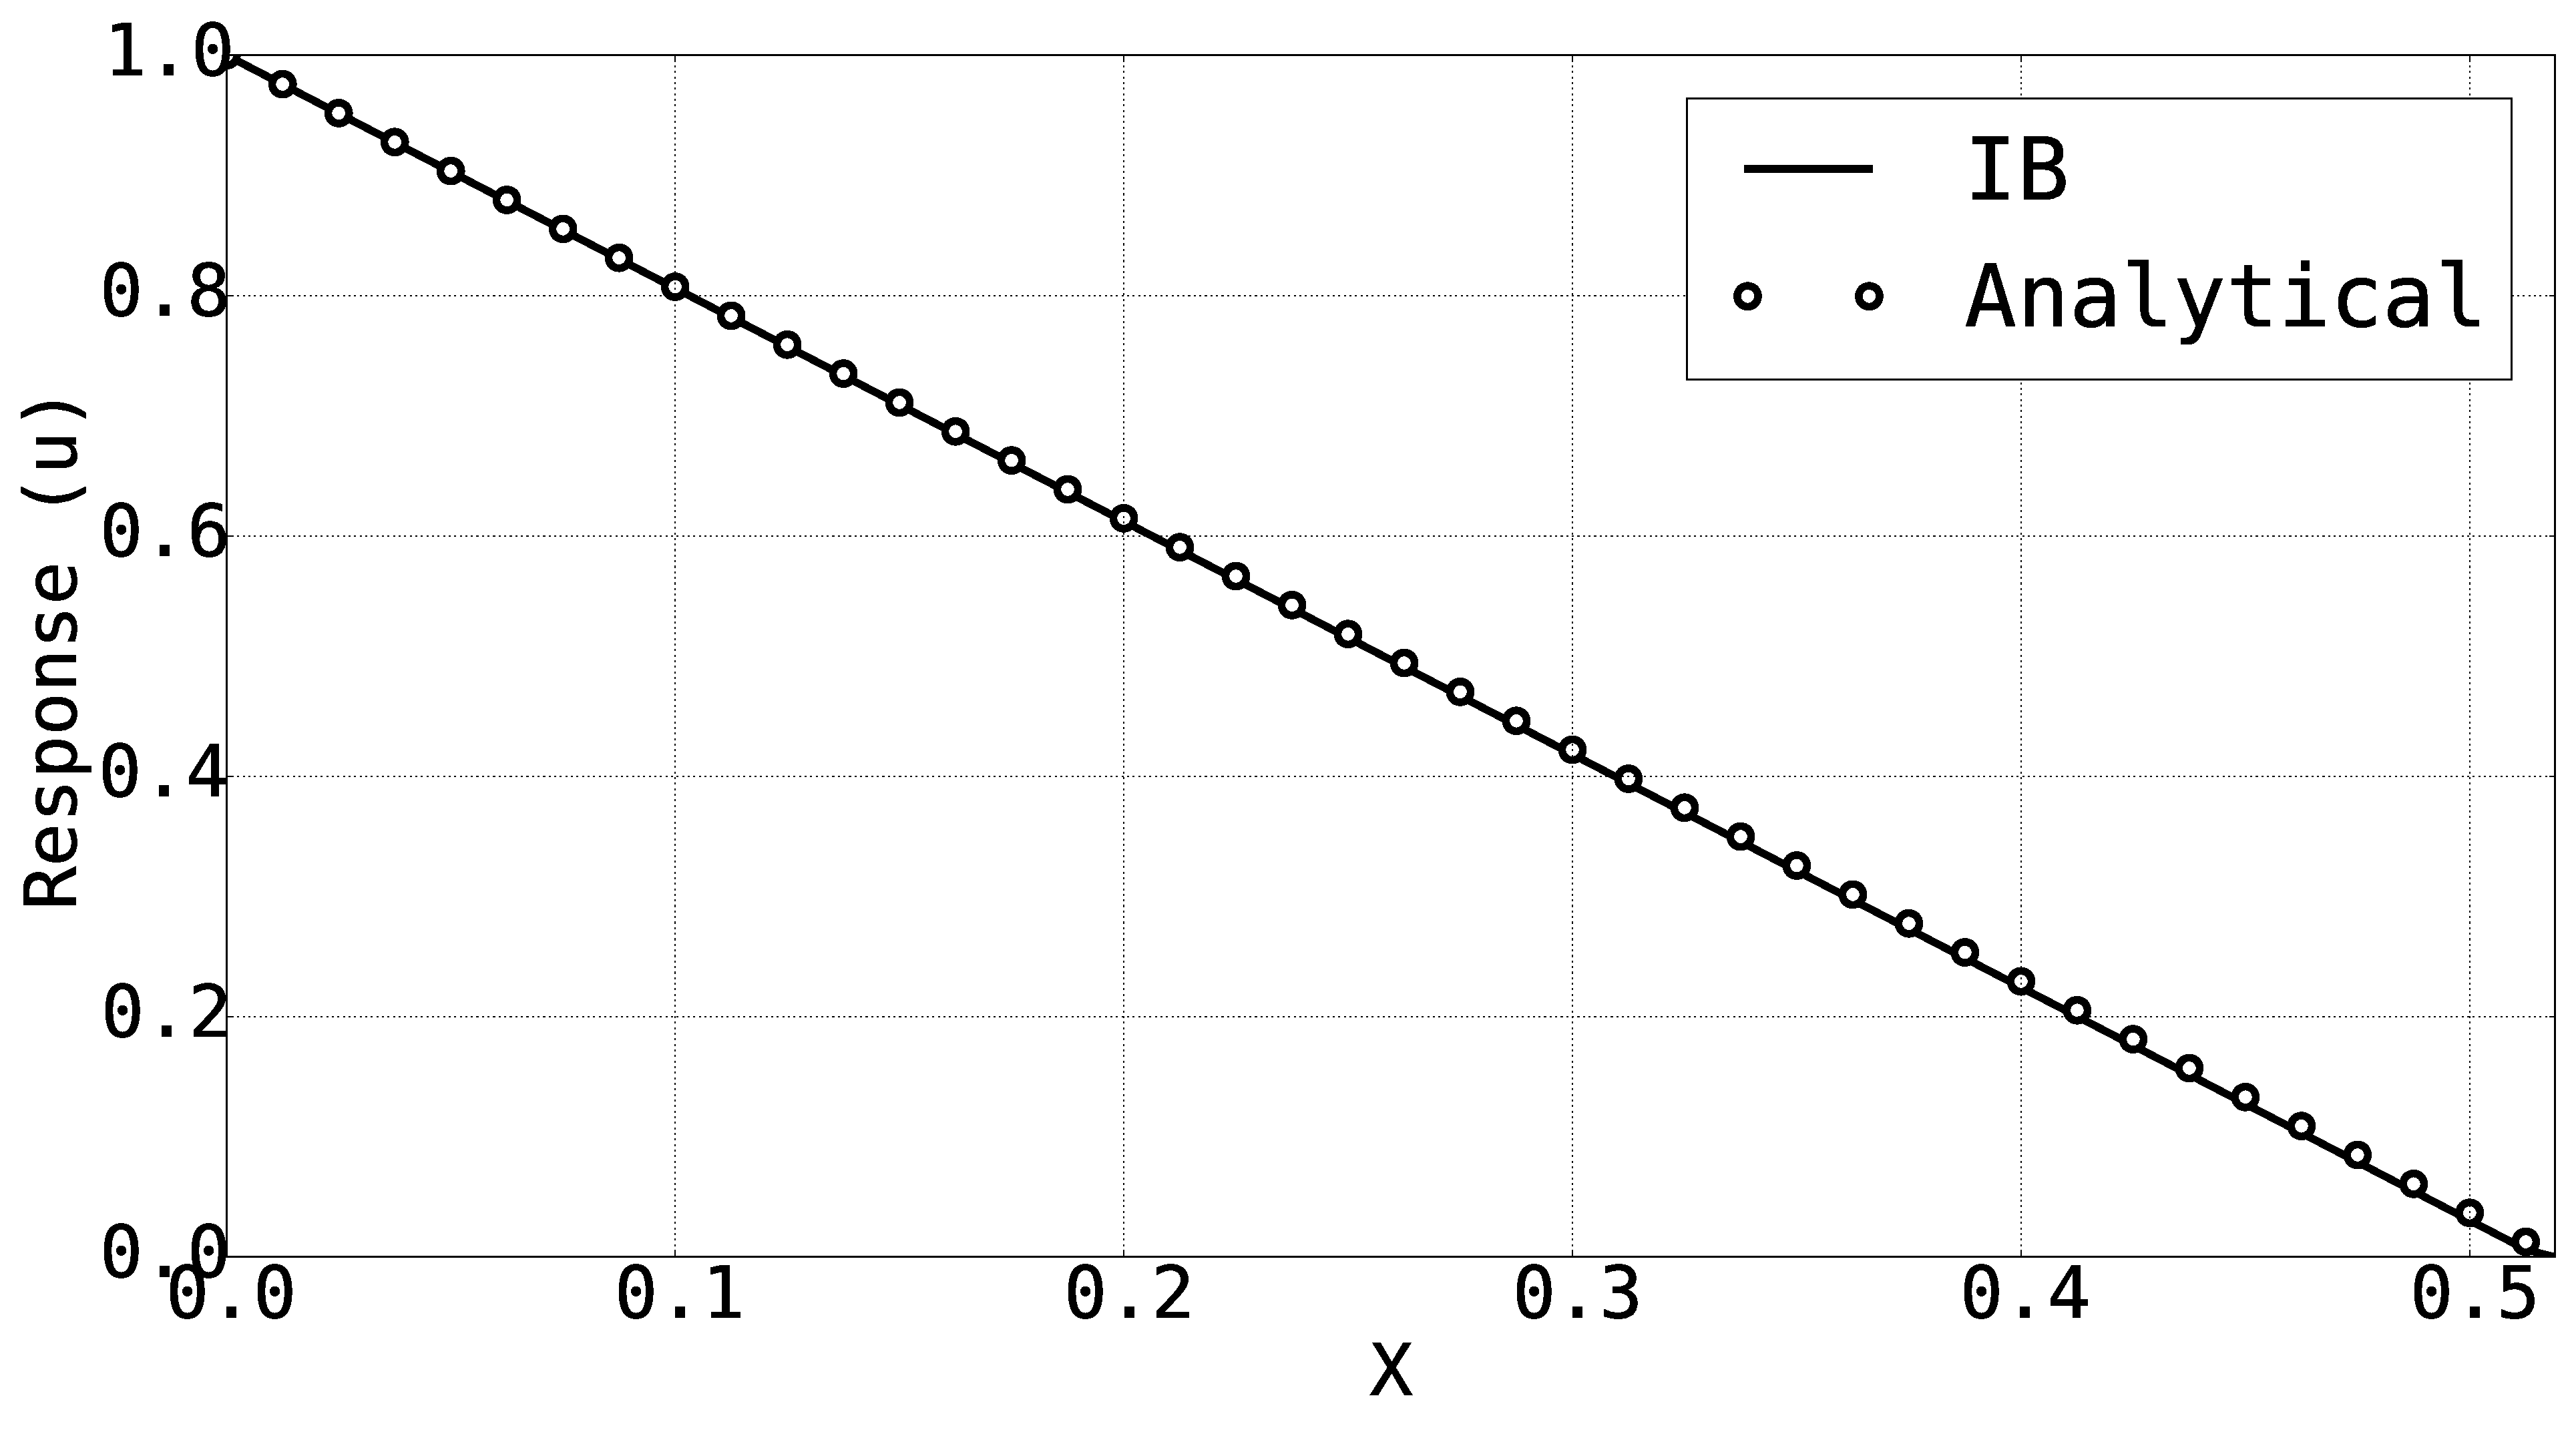
\includegraphics[width=7.0cm]{Chapter_3/figure/classicalIB_nodeNumber_2point_81.eps}
	}
	\quad
	\subfigure[N = 81, 4-point delta function]
	{
	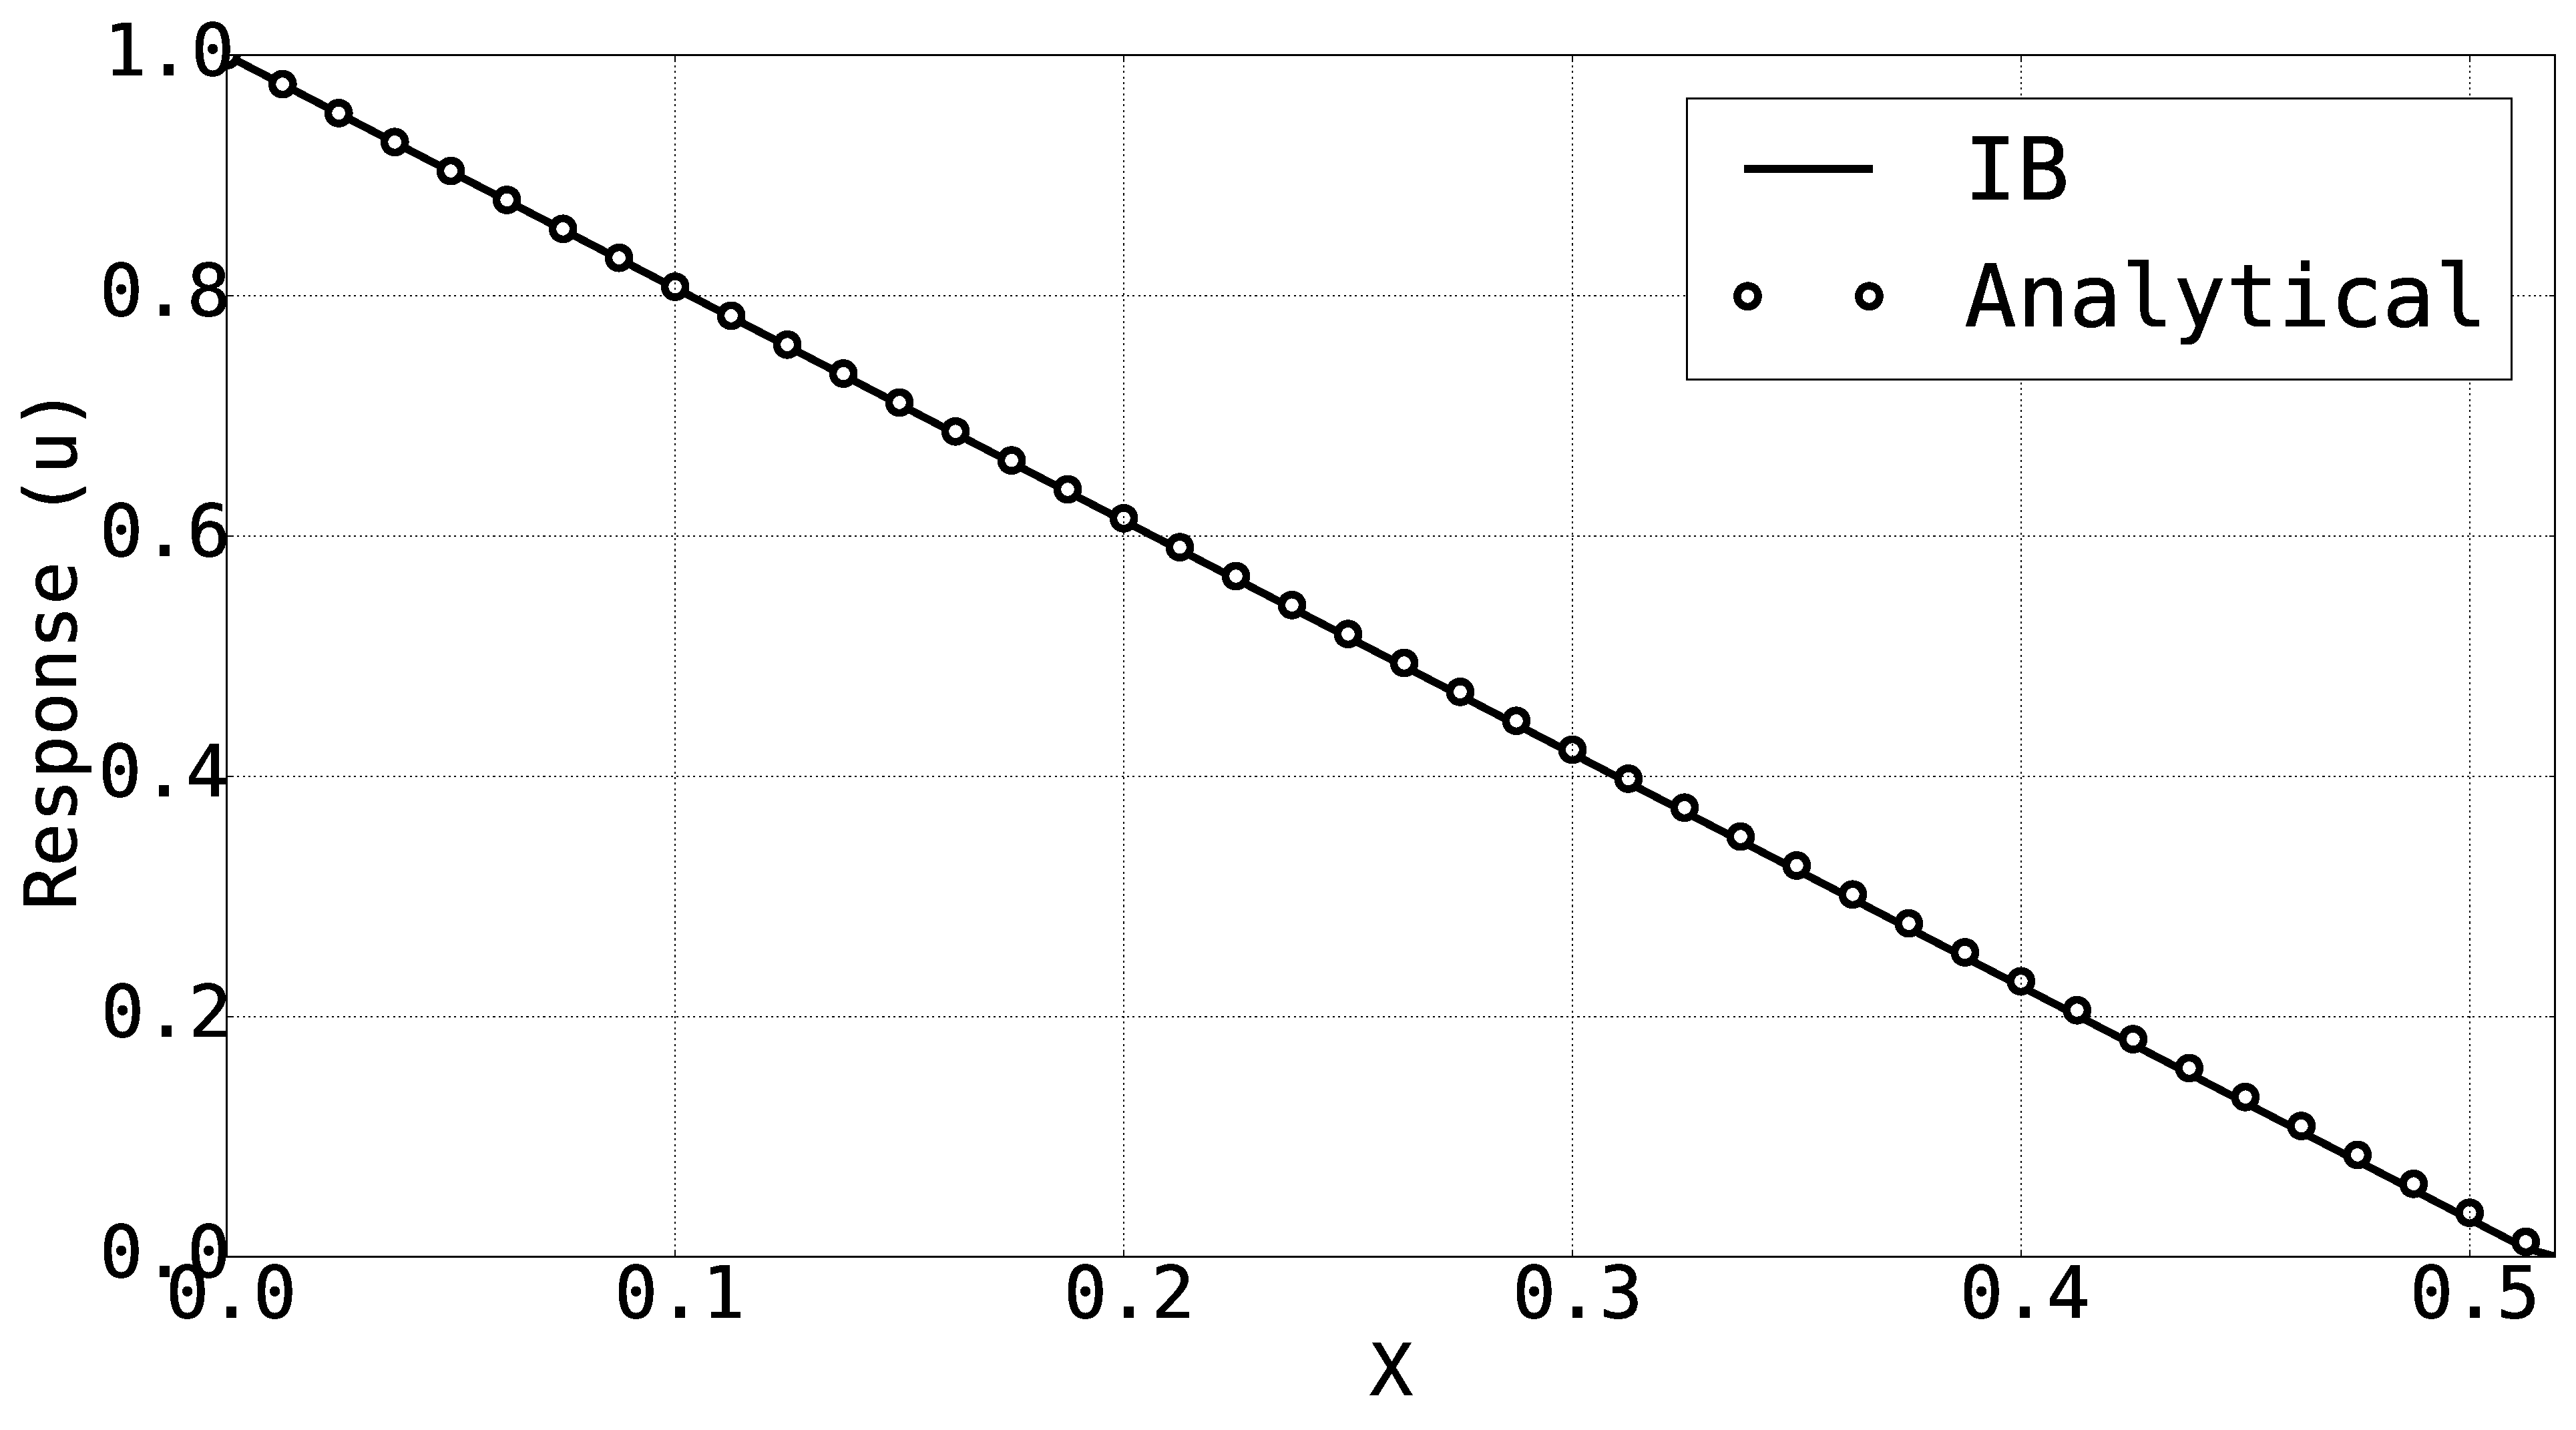
\includegraphics[width=7.0cm]{Chapter_3/figure/classicalIB_nodeNumber_4point_81.eps}
	}
	\\
	\subfigure[N = 161, 2-point delta function]
	{
	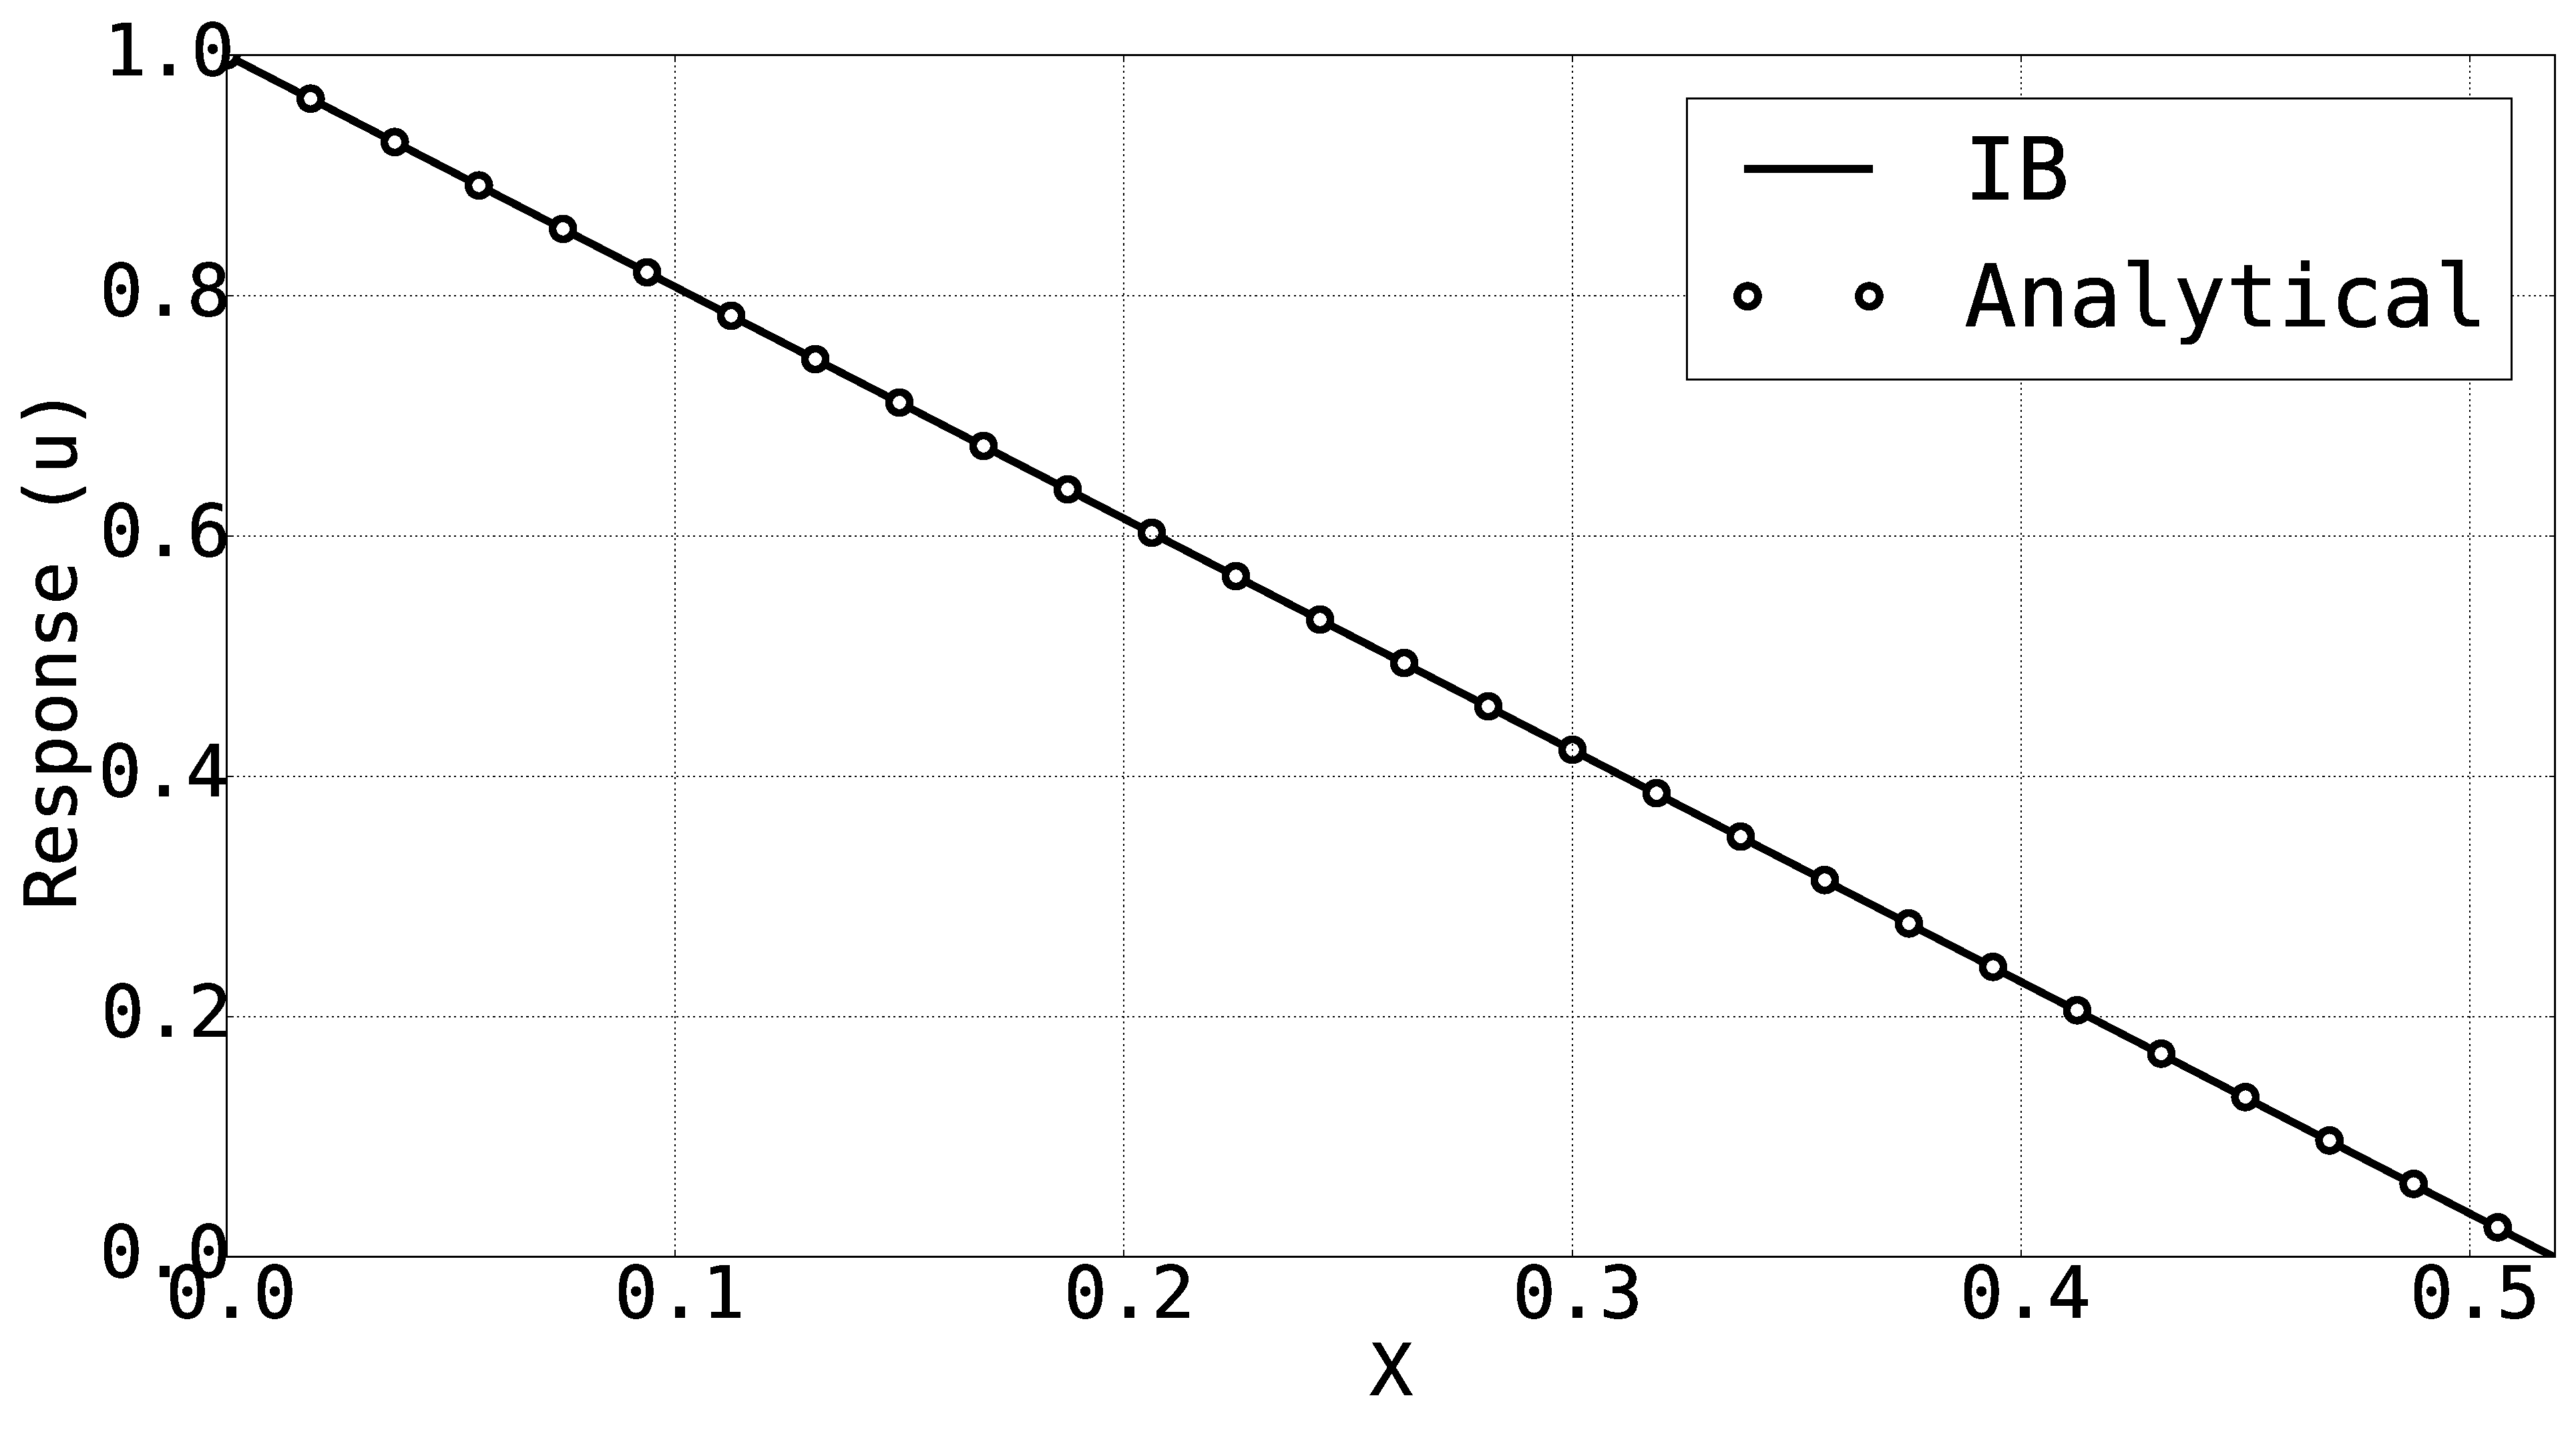
\includegraphics[width=7.0cm]{Chapter_3/figure/classicalIB_nodeNumber_2point_161.eps}
	}
	\quad
	\subfigure[N = 161, 4-point delta function]
	{
	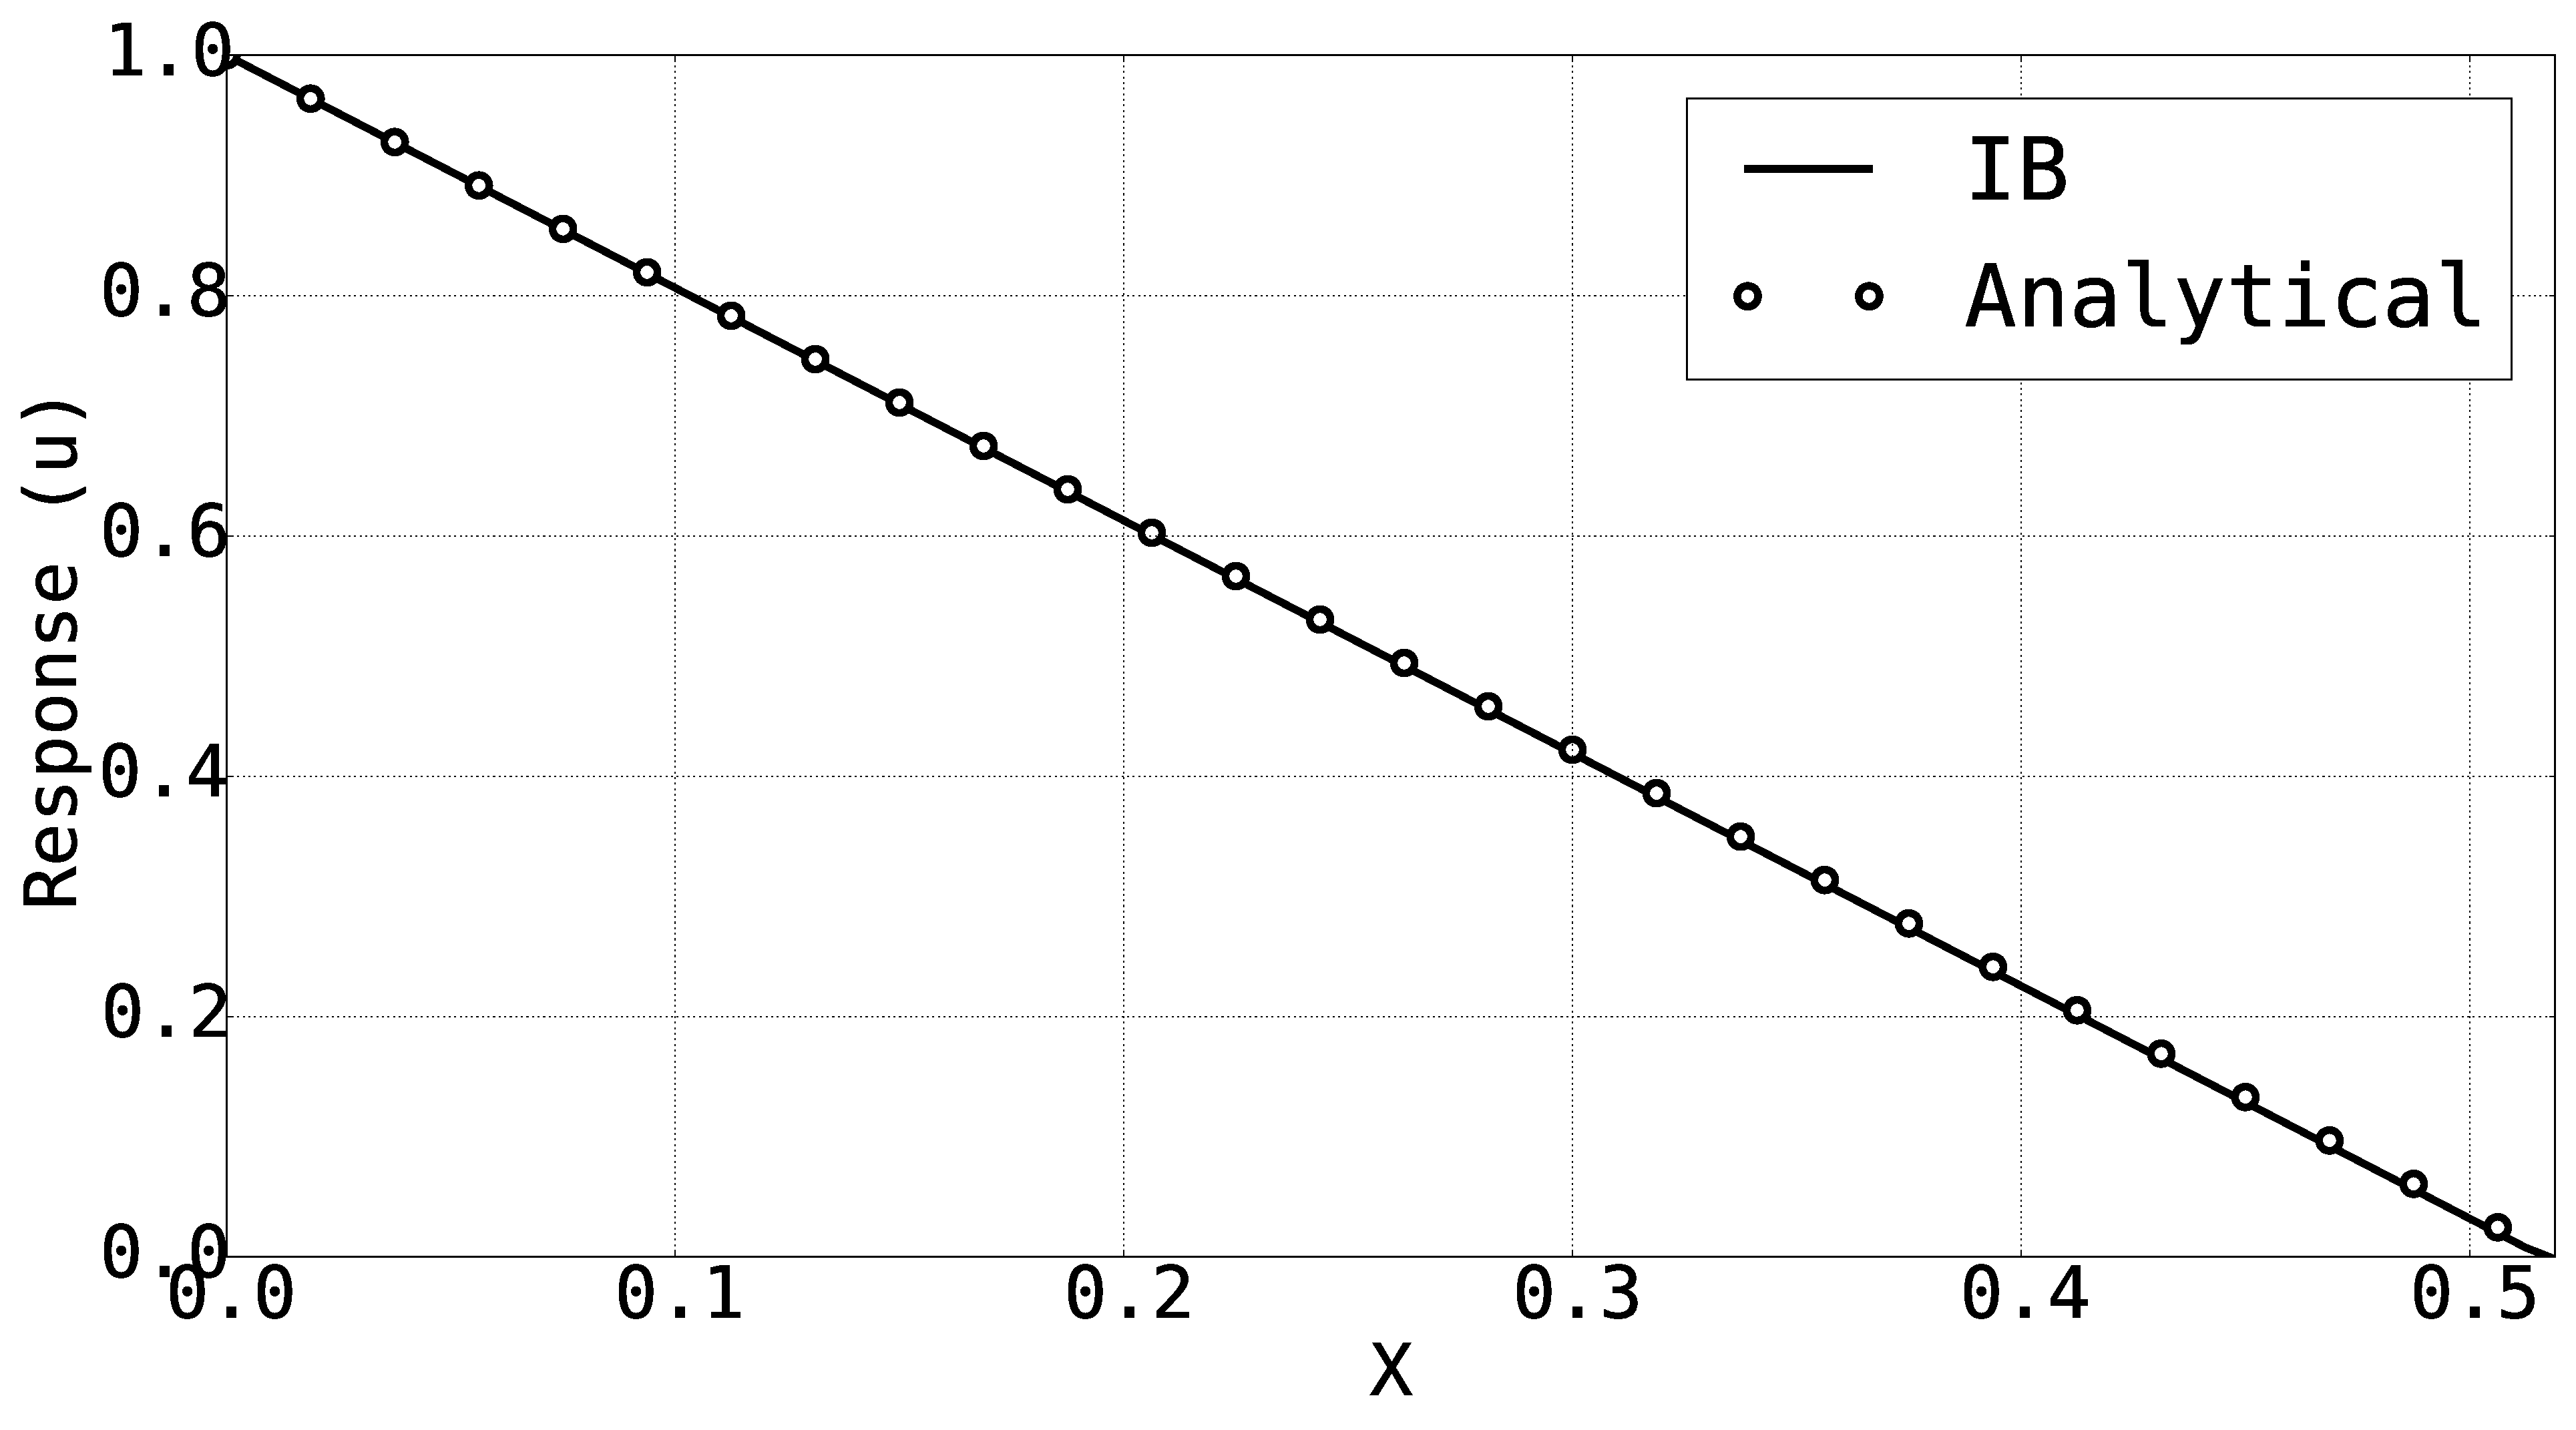
\includegraphics[width=7.0cm]{Chapter_3/figure/classicalIB_nodeNumber_4point_161.eps}
	}
	\caption{Comparison between IB and analytical results for different porosity values.}
	\label{fig:C3_classicalIBResultNodeNumber}
\end{figure}

\begin{table}[H]
\centering
\begin{tabular}{c | c | c}
	  & \multicolumn{2}{c}{RMSE value} \\ \hline
	 Node number & 2-point delta function & 4-point delta function \\ \hline \hline
	 11 & 0.0105 & 0.0292 \\ \hline
	 41 & 0.0035 & 0.002 \\ \hline
	 81 & 0.0026 & 0.0022 \\ \hline
	 161 & 0.00023 & 0.0002 \\
\end{tabular}
\caption{RMSE value for different node numbers and delta functions.}
\label{table:C3_classicalIBResultNodeNumberRMSE}
\end{table}

As shown in Figure \ref{fig:C3_classicalIBResultNodeNumber} and Table \ref{table:C3_classicalIBResultNodeNumberRMSE}, by increasing the number of nodes, the error in IB result decreases. However, changing the delta function from 2-point to 4-point does not effect the accuracy of the solution significantly. The higher order delta function can also decreases the accuracy of the solution for very low number of nodes (here 11). 

For the second investigation, we looked at the effect of changing the moving wall velocity on the solution accuracy. For this simulation, we fixed the number of nodes to 81 and set the stiffness value to $10^2$. The wall location is fixed at $0.51885$. The time step is also chosen as $10^{-5}$. For this problem, we only focused on 2-point delta function. We chose the wall velocity as $10$, $10^2$, $10^3$, and $10^4$. As shown in Figure \ref{fig:C3_classicalIBResultWallVelocity} and Table \ref{fig:C3_classicalIBResultWallVelocityRMSE}, the method is capable of handling flow with different velocity without a loss in accuracy of the results. However, the simulation time increases with increase in wall velocity.

\begin{figure}[H]
	\centering
	\subfigure[$u_{wall} = 10 m/s$]
	{
	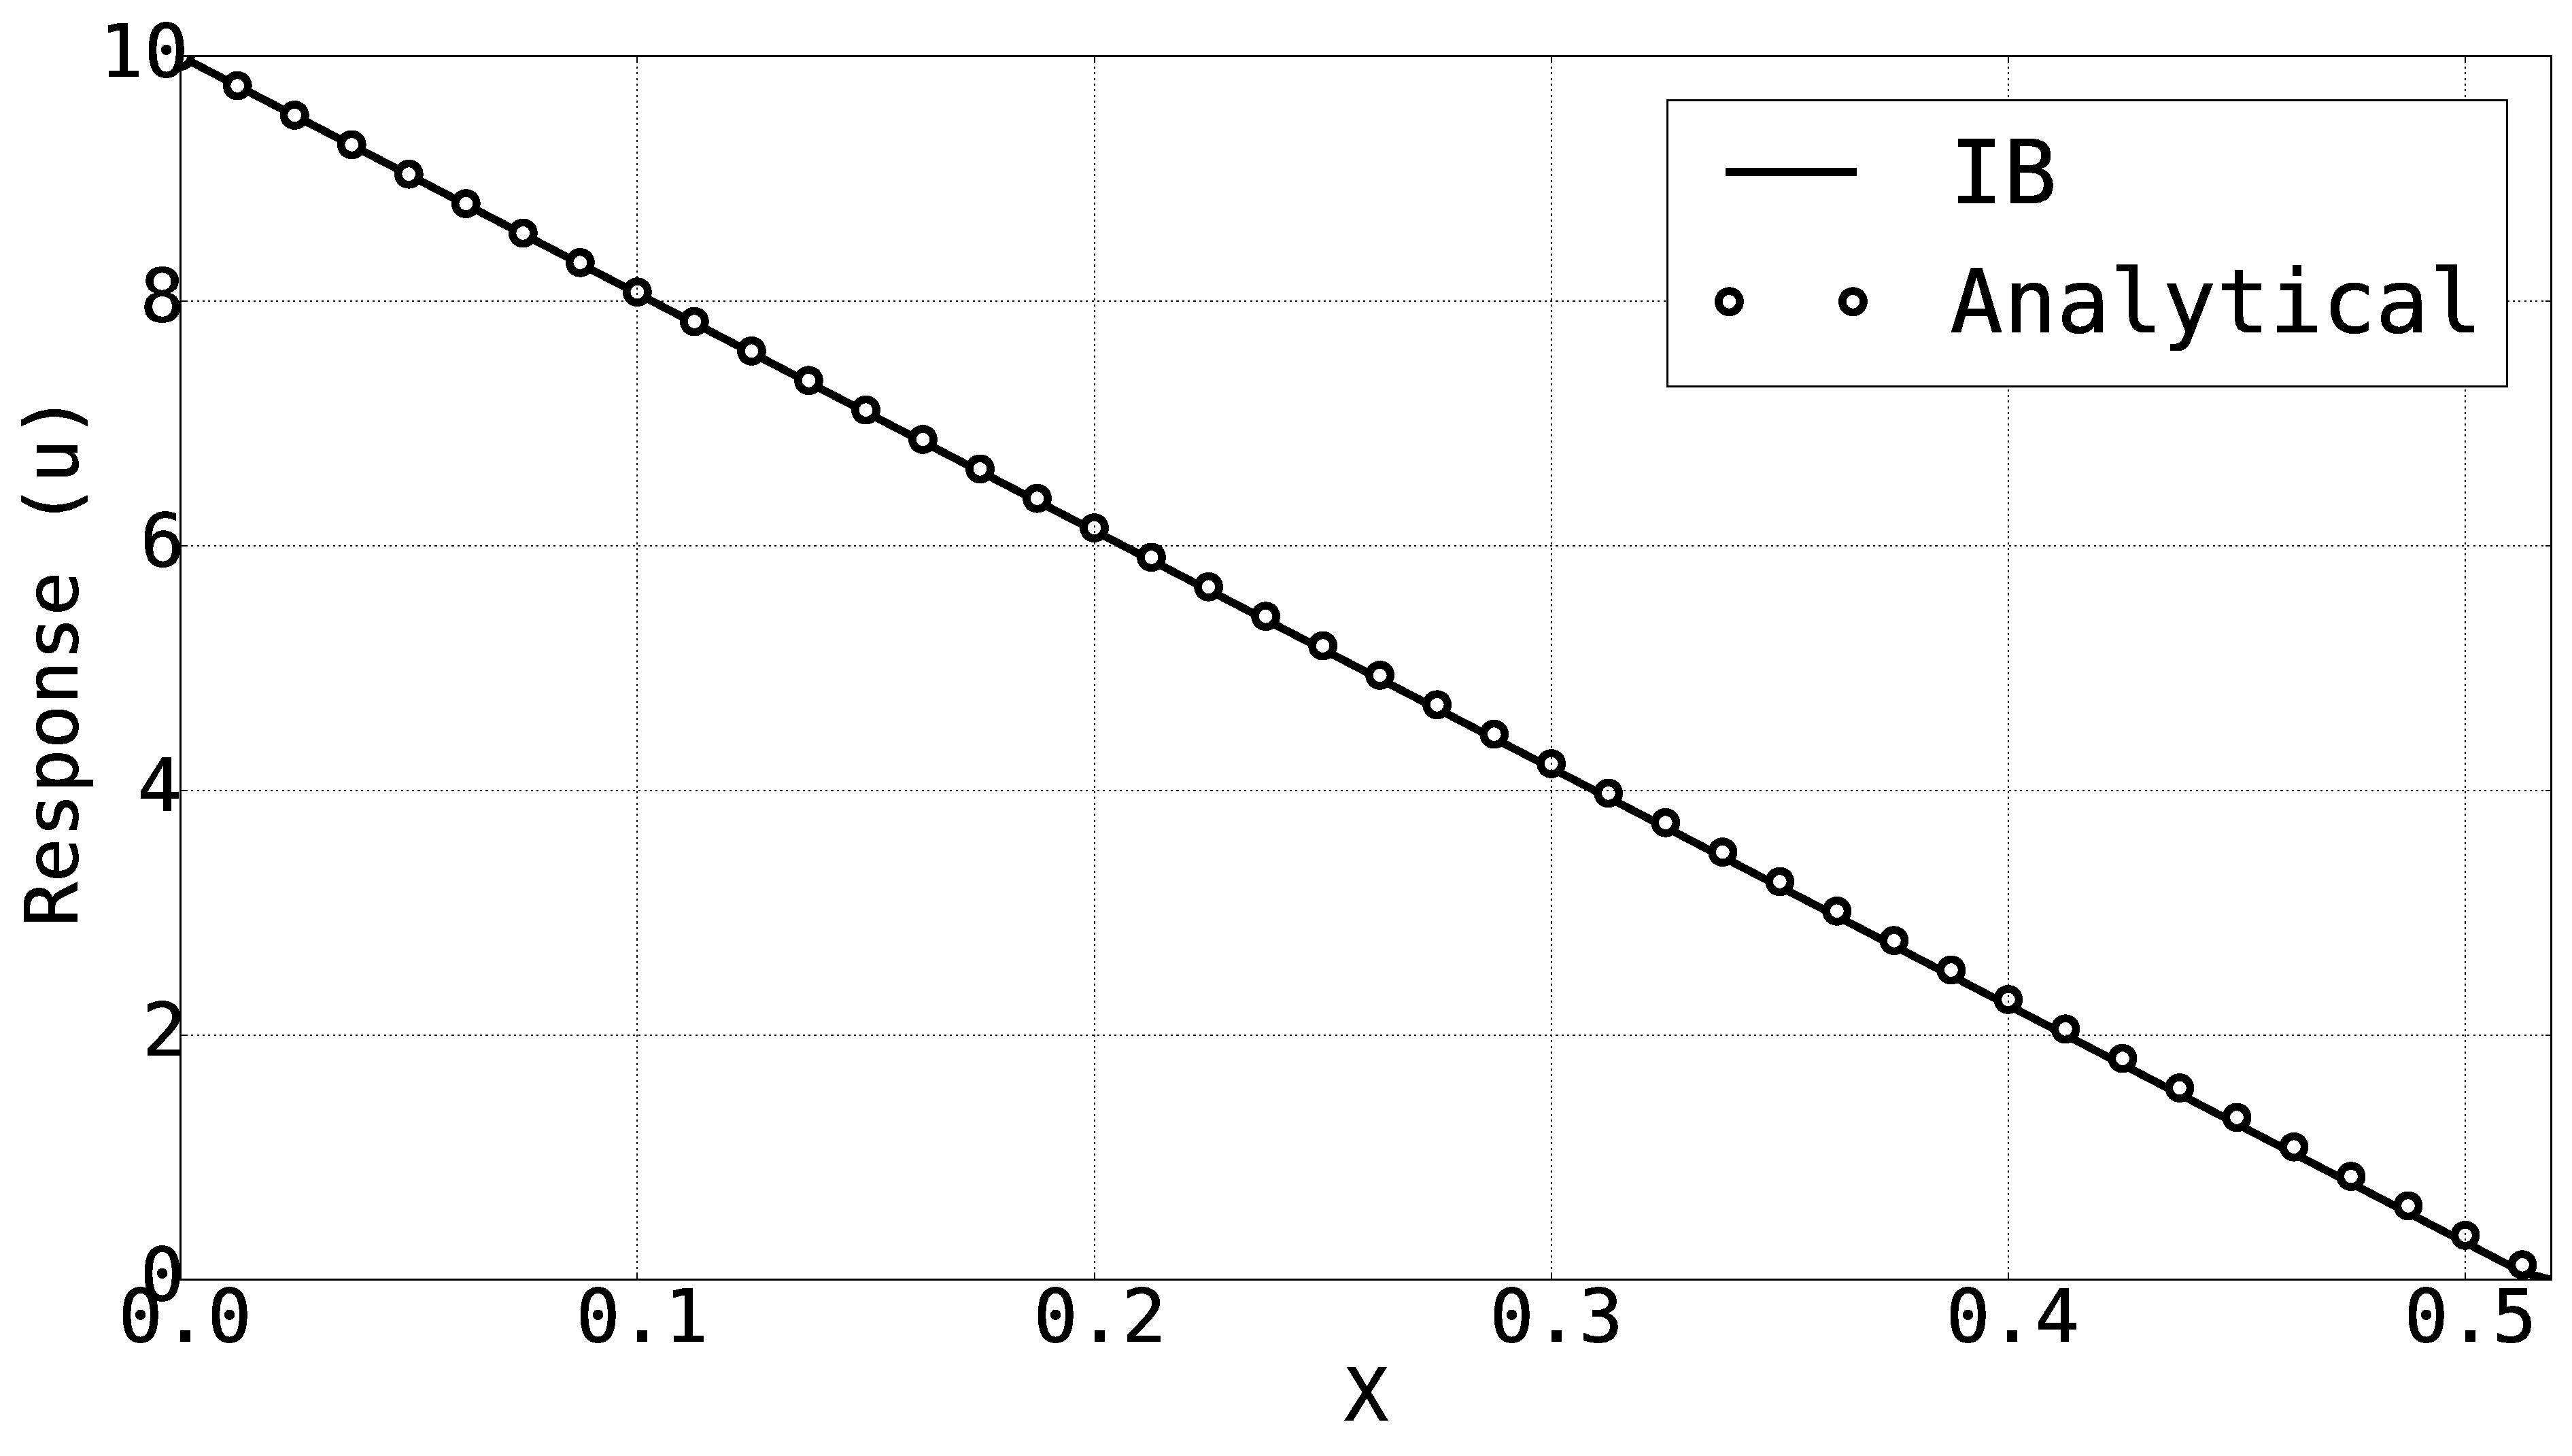
\includegraphics[width=7.0cm]{Chapter_3/figure/classicalIB_wallVelocity_2point_10.eps}
	}
	\quad
	\subfigure[$u_{wall} = 10^2 m/s$]
	{
	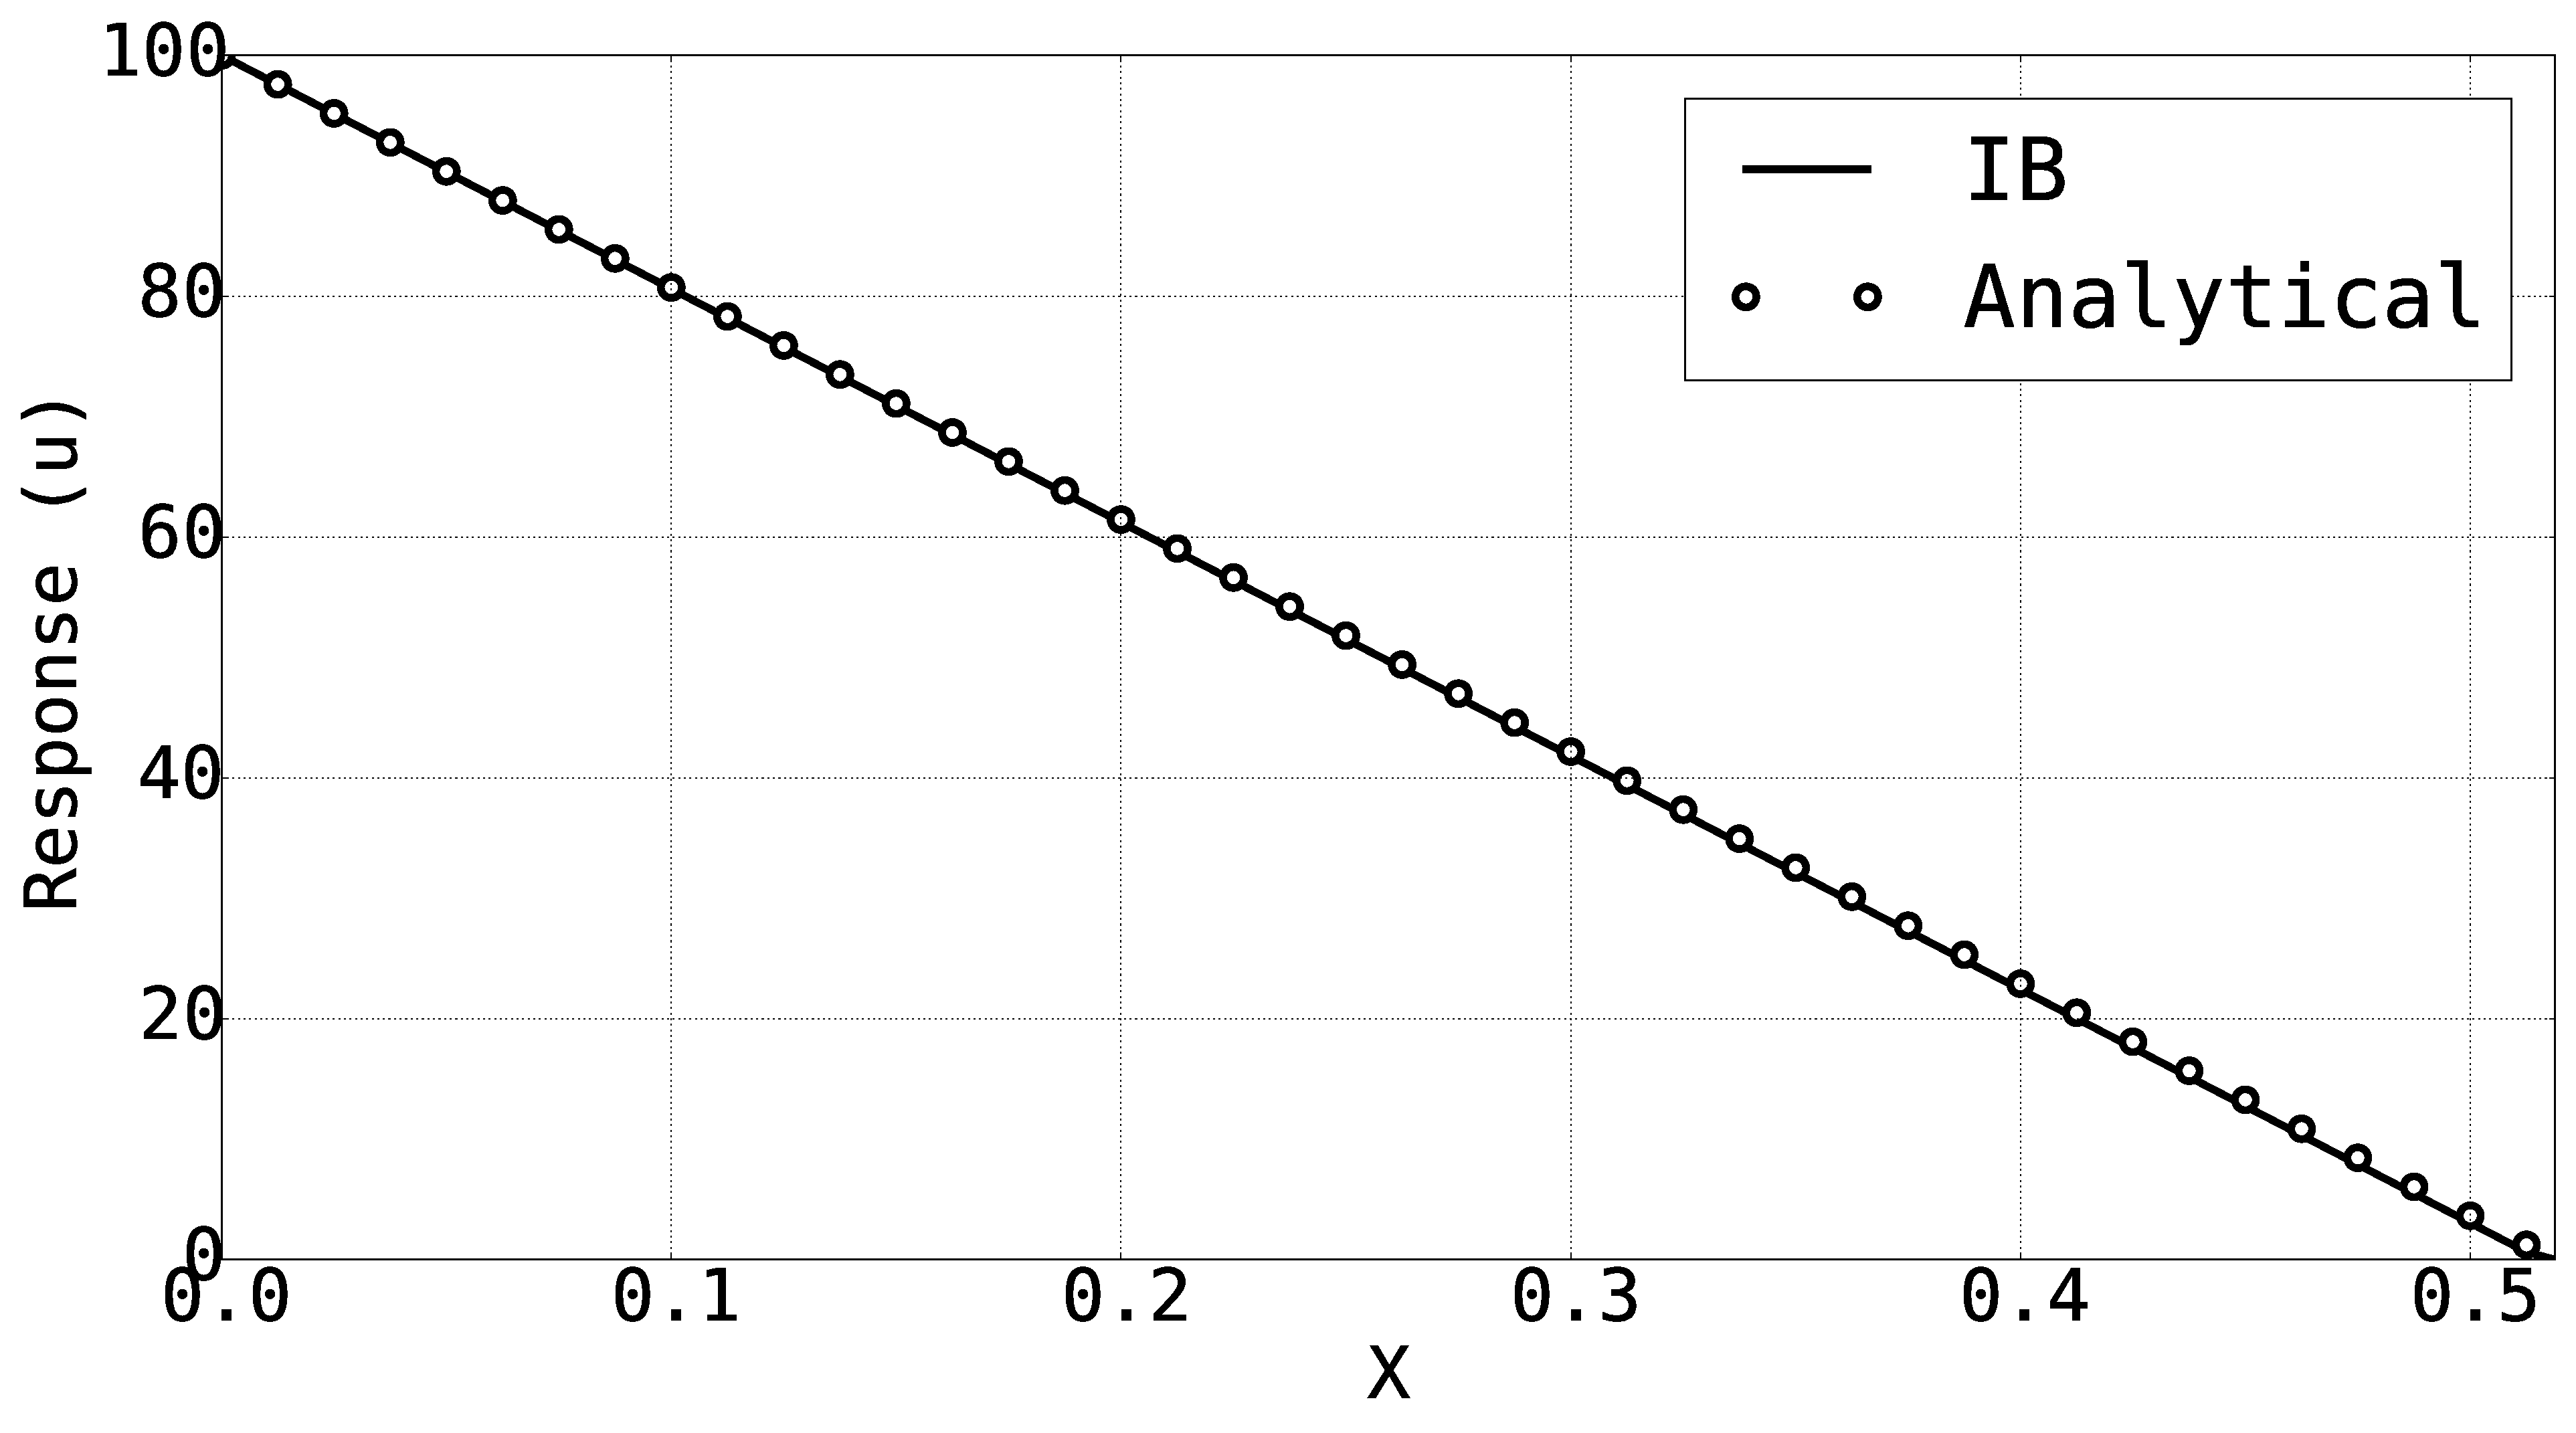
\includegraphics[width=7.0cm]{Chapter_3/figure/classicalIB_wallVelocity_2point_100.eps}
	}
	\\
	\subfigure[$u_{wall} = 10^3 m/s$]
	{
	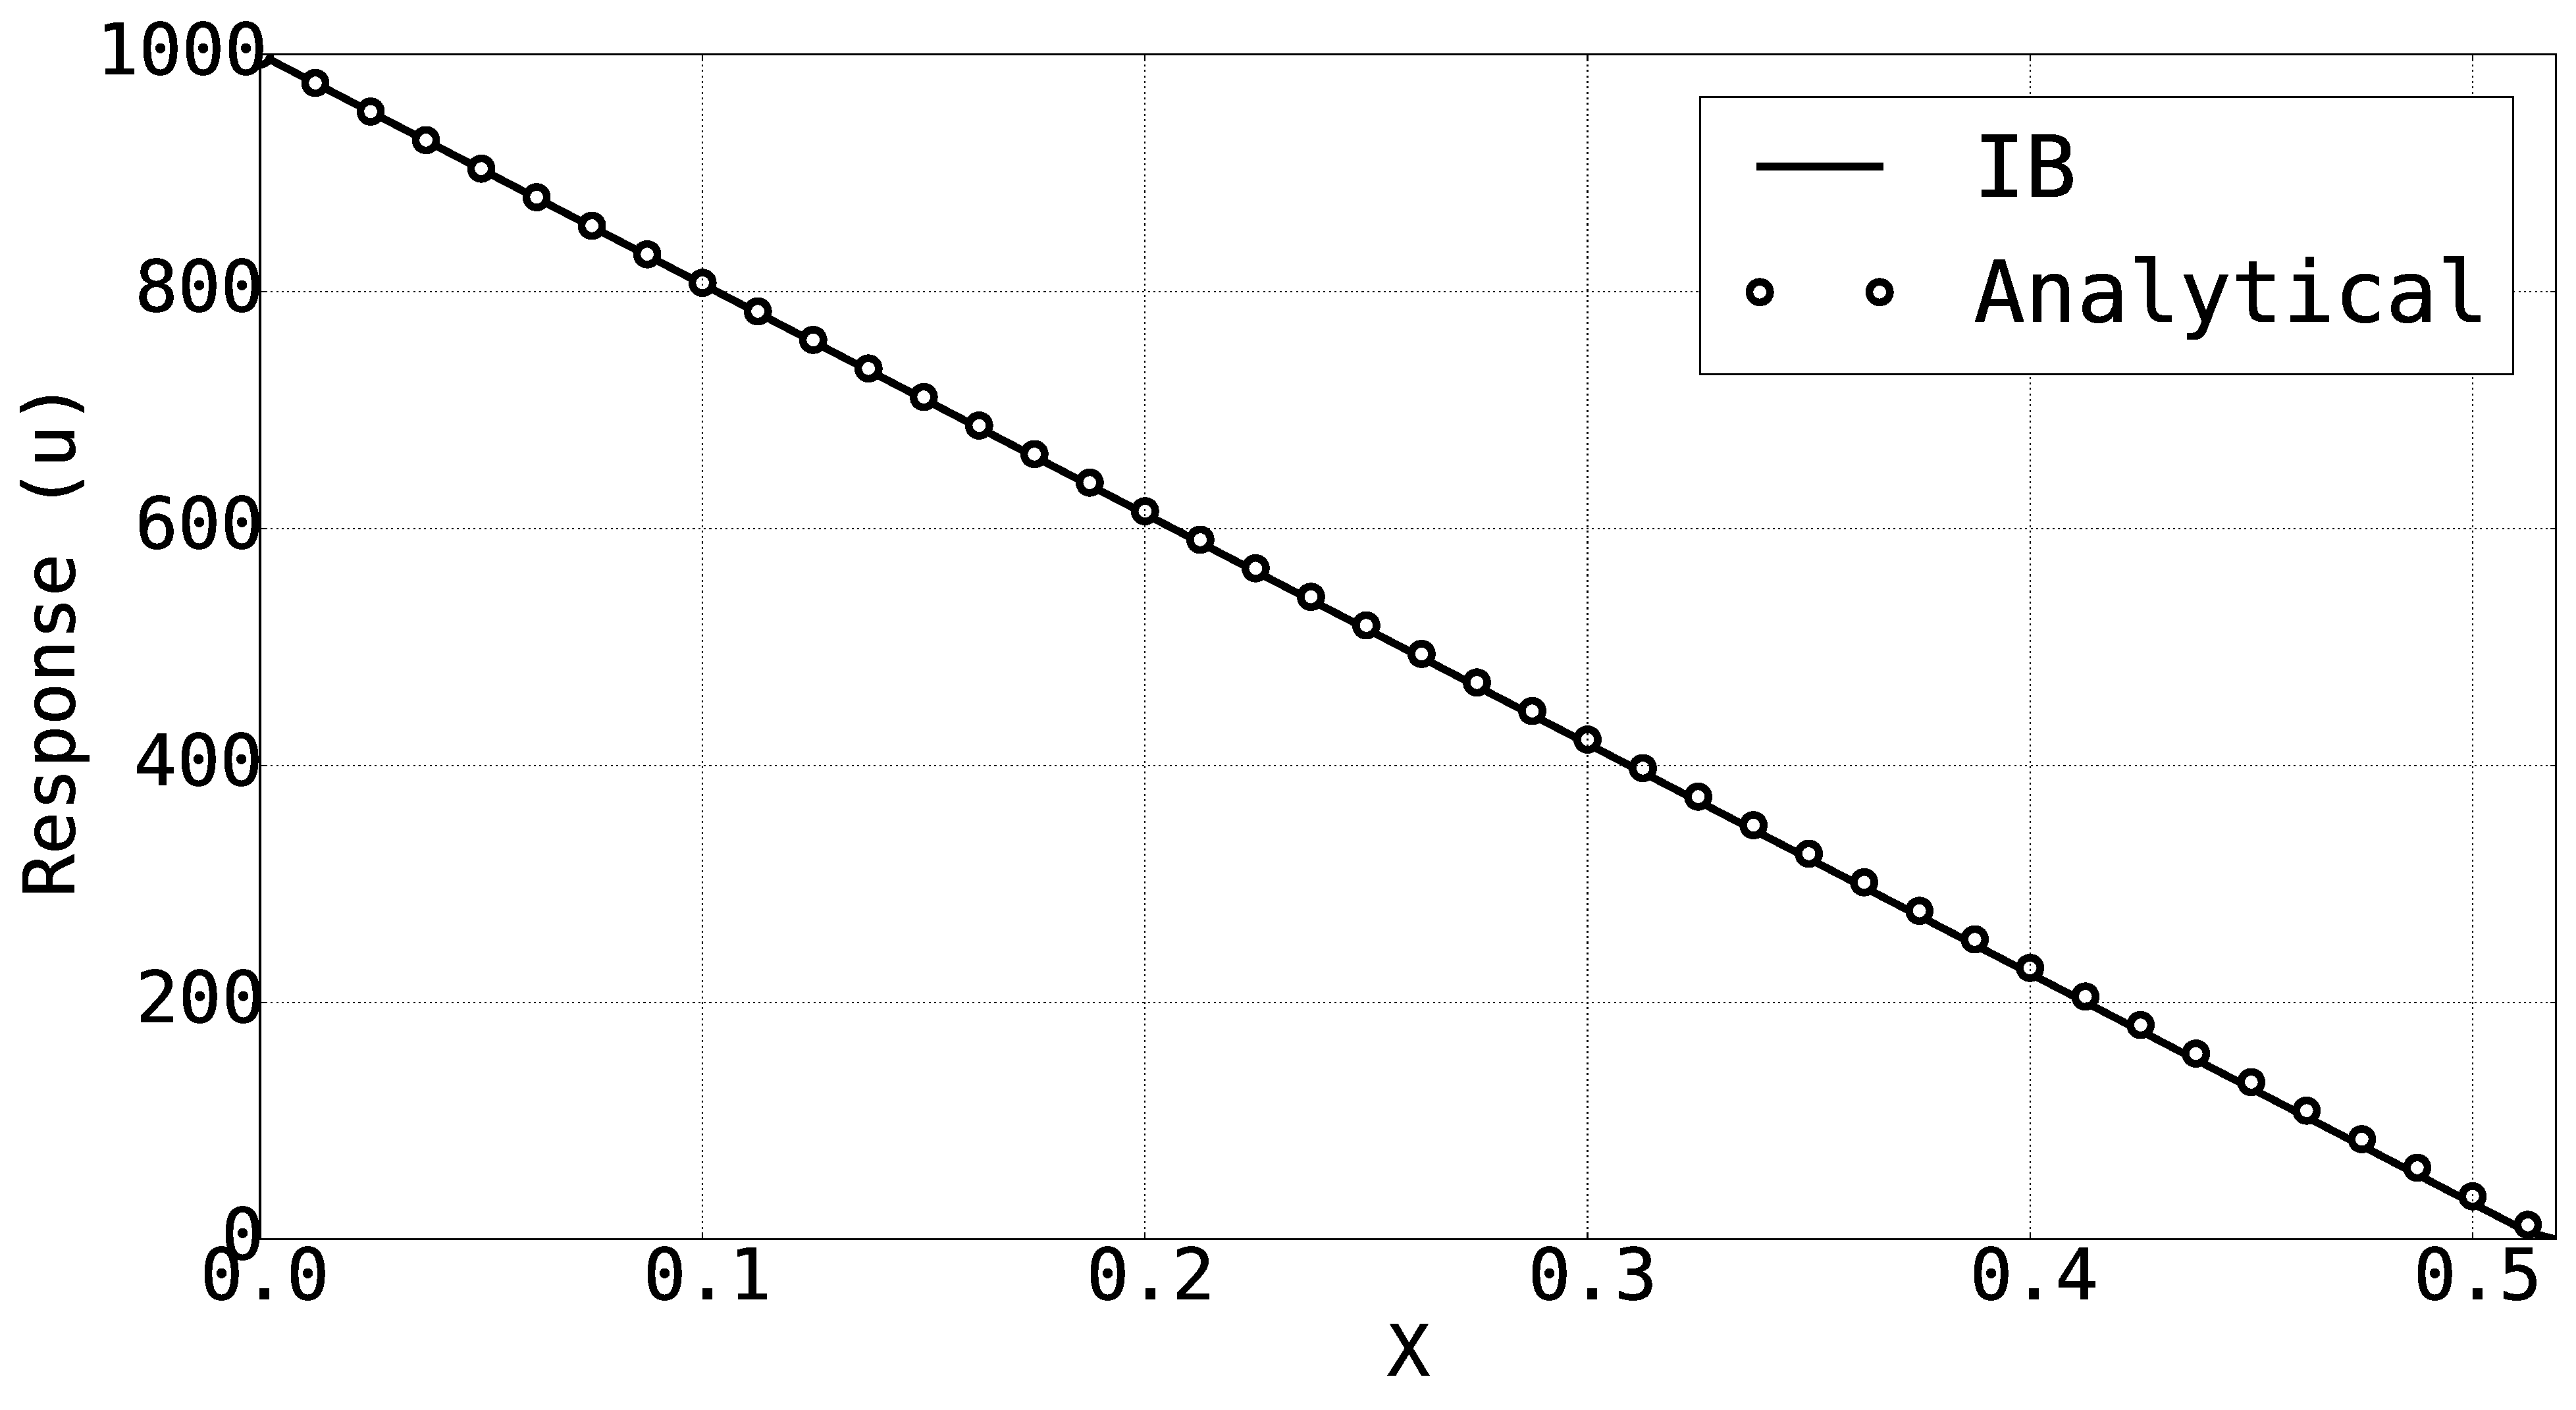
\includegraphics[width=7.0cm]{Chapter_3/figure/classicalIB_wallVelocity_2point_1000.eps}
	}
	\quad
	\subfigure[$u_{wall} = 10^4 m/s$]
	{
	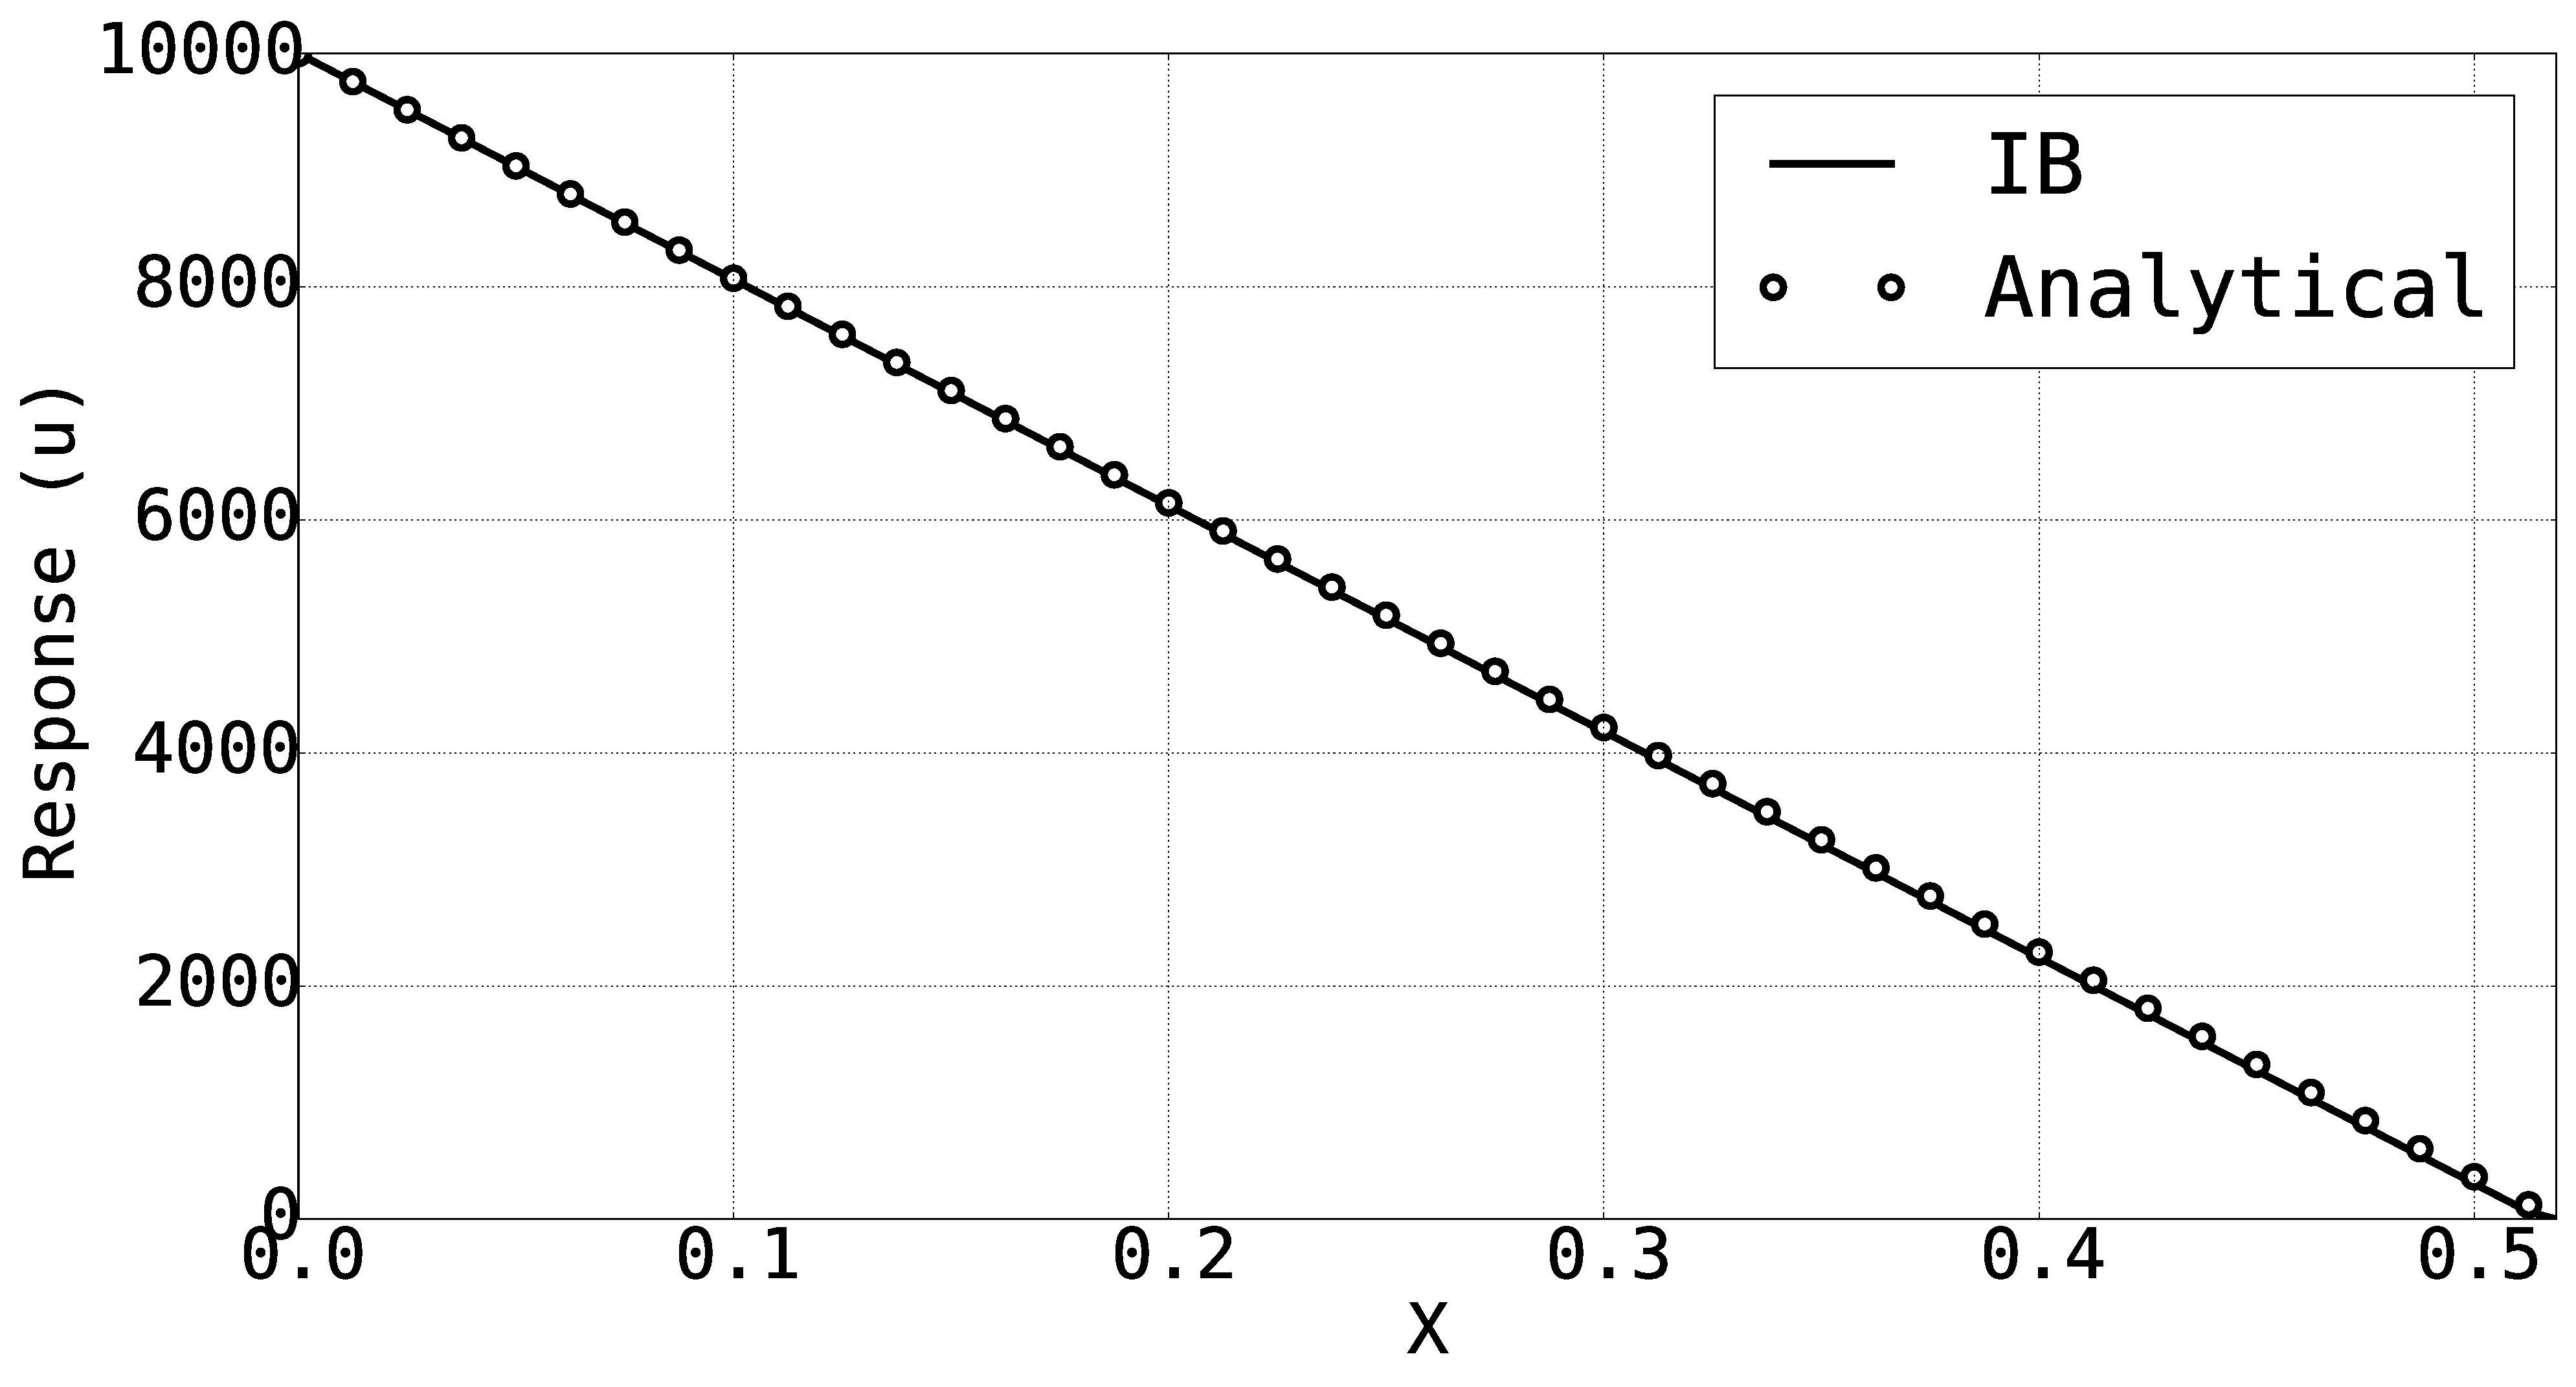
\includegraphics[width=7.0cm]{Chapter_3/figure/classicalIB_wallVelocity_2point_10000.eps}
	}
	\caption{Comparison between IB and analytical results for different wall velocities.}
	\label{fig:C3_classicalIBResultWallVelocity}
\end{figure}

\begin{table}[H]
\centering
\begin{tabular}{c | c}
	 Wall velocity & RMSE \\ \hline \hline
	 10 & 0.0024\\ \hline
	 $10^2$ & 0.0024 \\ \hline
	 $10^3$ & 0.0024 \\ \hline
	 $10^4$ & 0.0024 \\
\end{tabular}
\caption{RMSE value for different wall velocities.}
\label{table:C3_classicalIBResultWallVelocityRMSE}
\end{table}

For the last case study of classical IB method, we looked at the effect of the wall stiffness on the accuracy of the solution. For this case, we fixed the wall location at $x_{wall} = 0.51885$ and defined the wall velocity as $10 m/s$. The time step is selected as $10^{-5}$. We looked at the wall stiffness of $0.1$, $1$, $10$, and $100$. As shown in Figure \ref{fig:C3_classicalIBResultWallStiffness} and Table \ref{table:C3_classicalIBResultWallStiffnessRMSE}, wall stiffness has a considerable effect of the solution result. Therefore, a convergence study for the wall stiffness value is usually required if one wants to model the stiff boundaries.

\begin{figure}[H]
	\centering
	\subfigure[$K_{wall} = 0.1$]
	{
	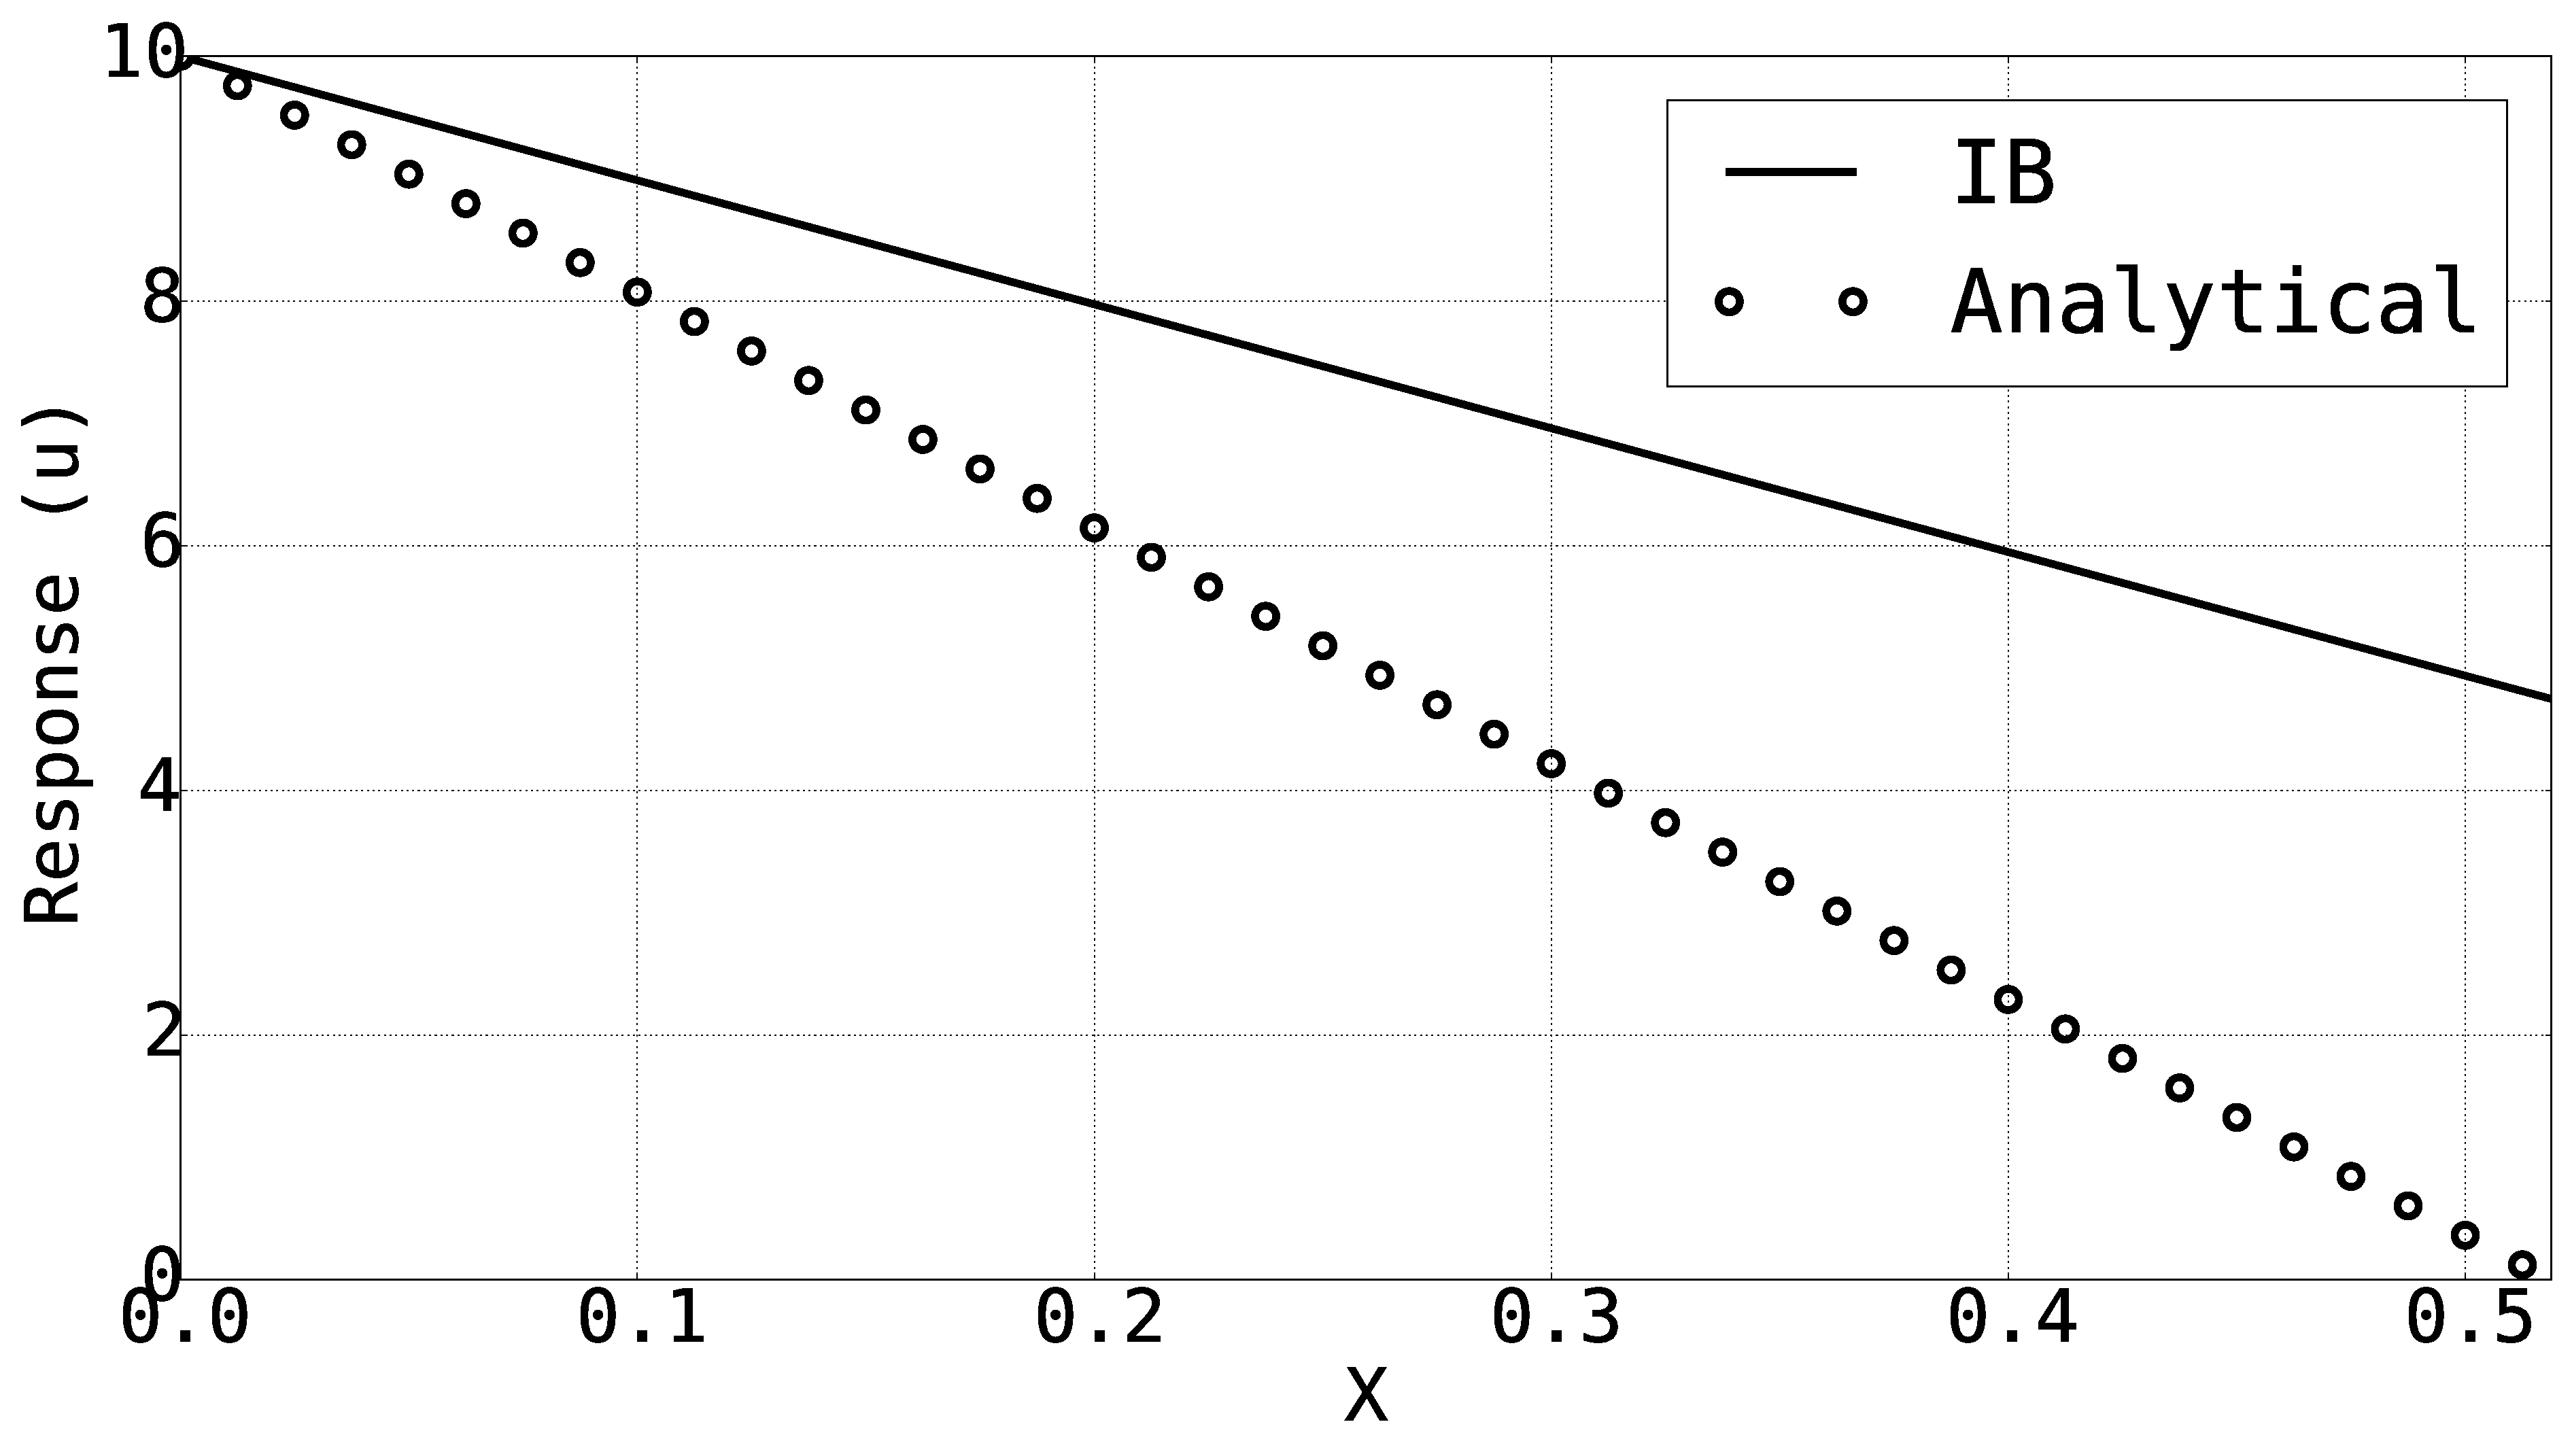
\includegraphics[width=7.0cm]{Chapter_3/figure/classicalIB_wallStiffness_2point_01.eps}
	}
	\quad
	\subfigure[$K_{wall} = 1$]
	{
	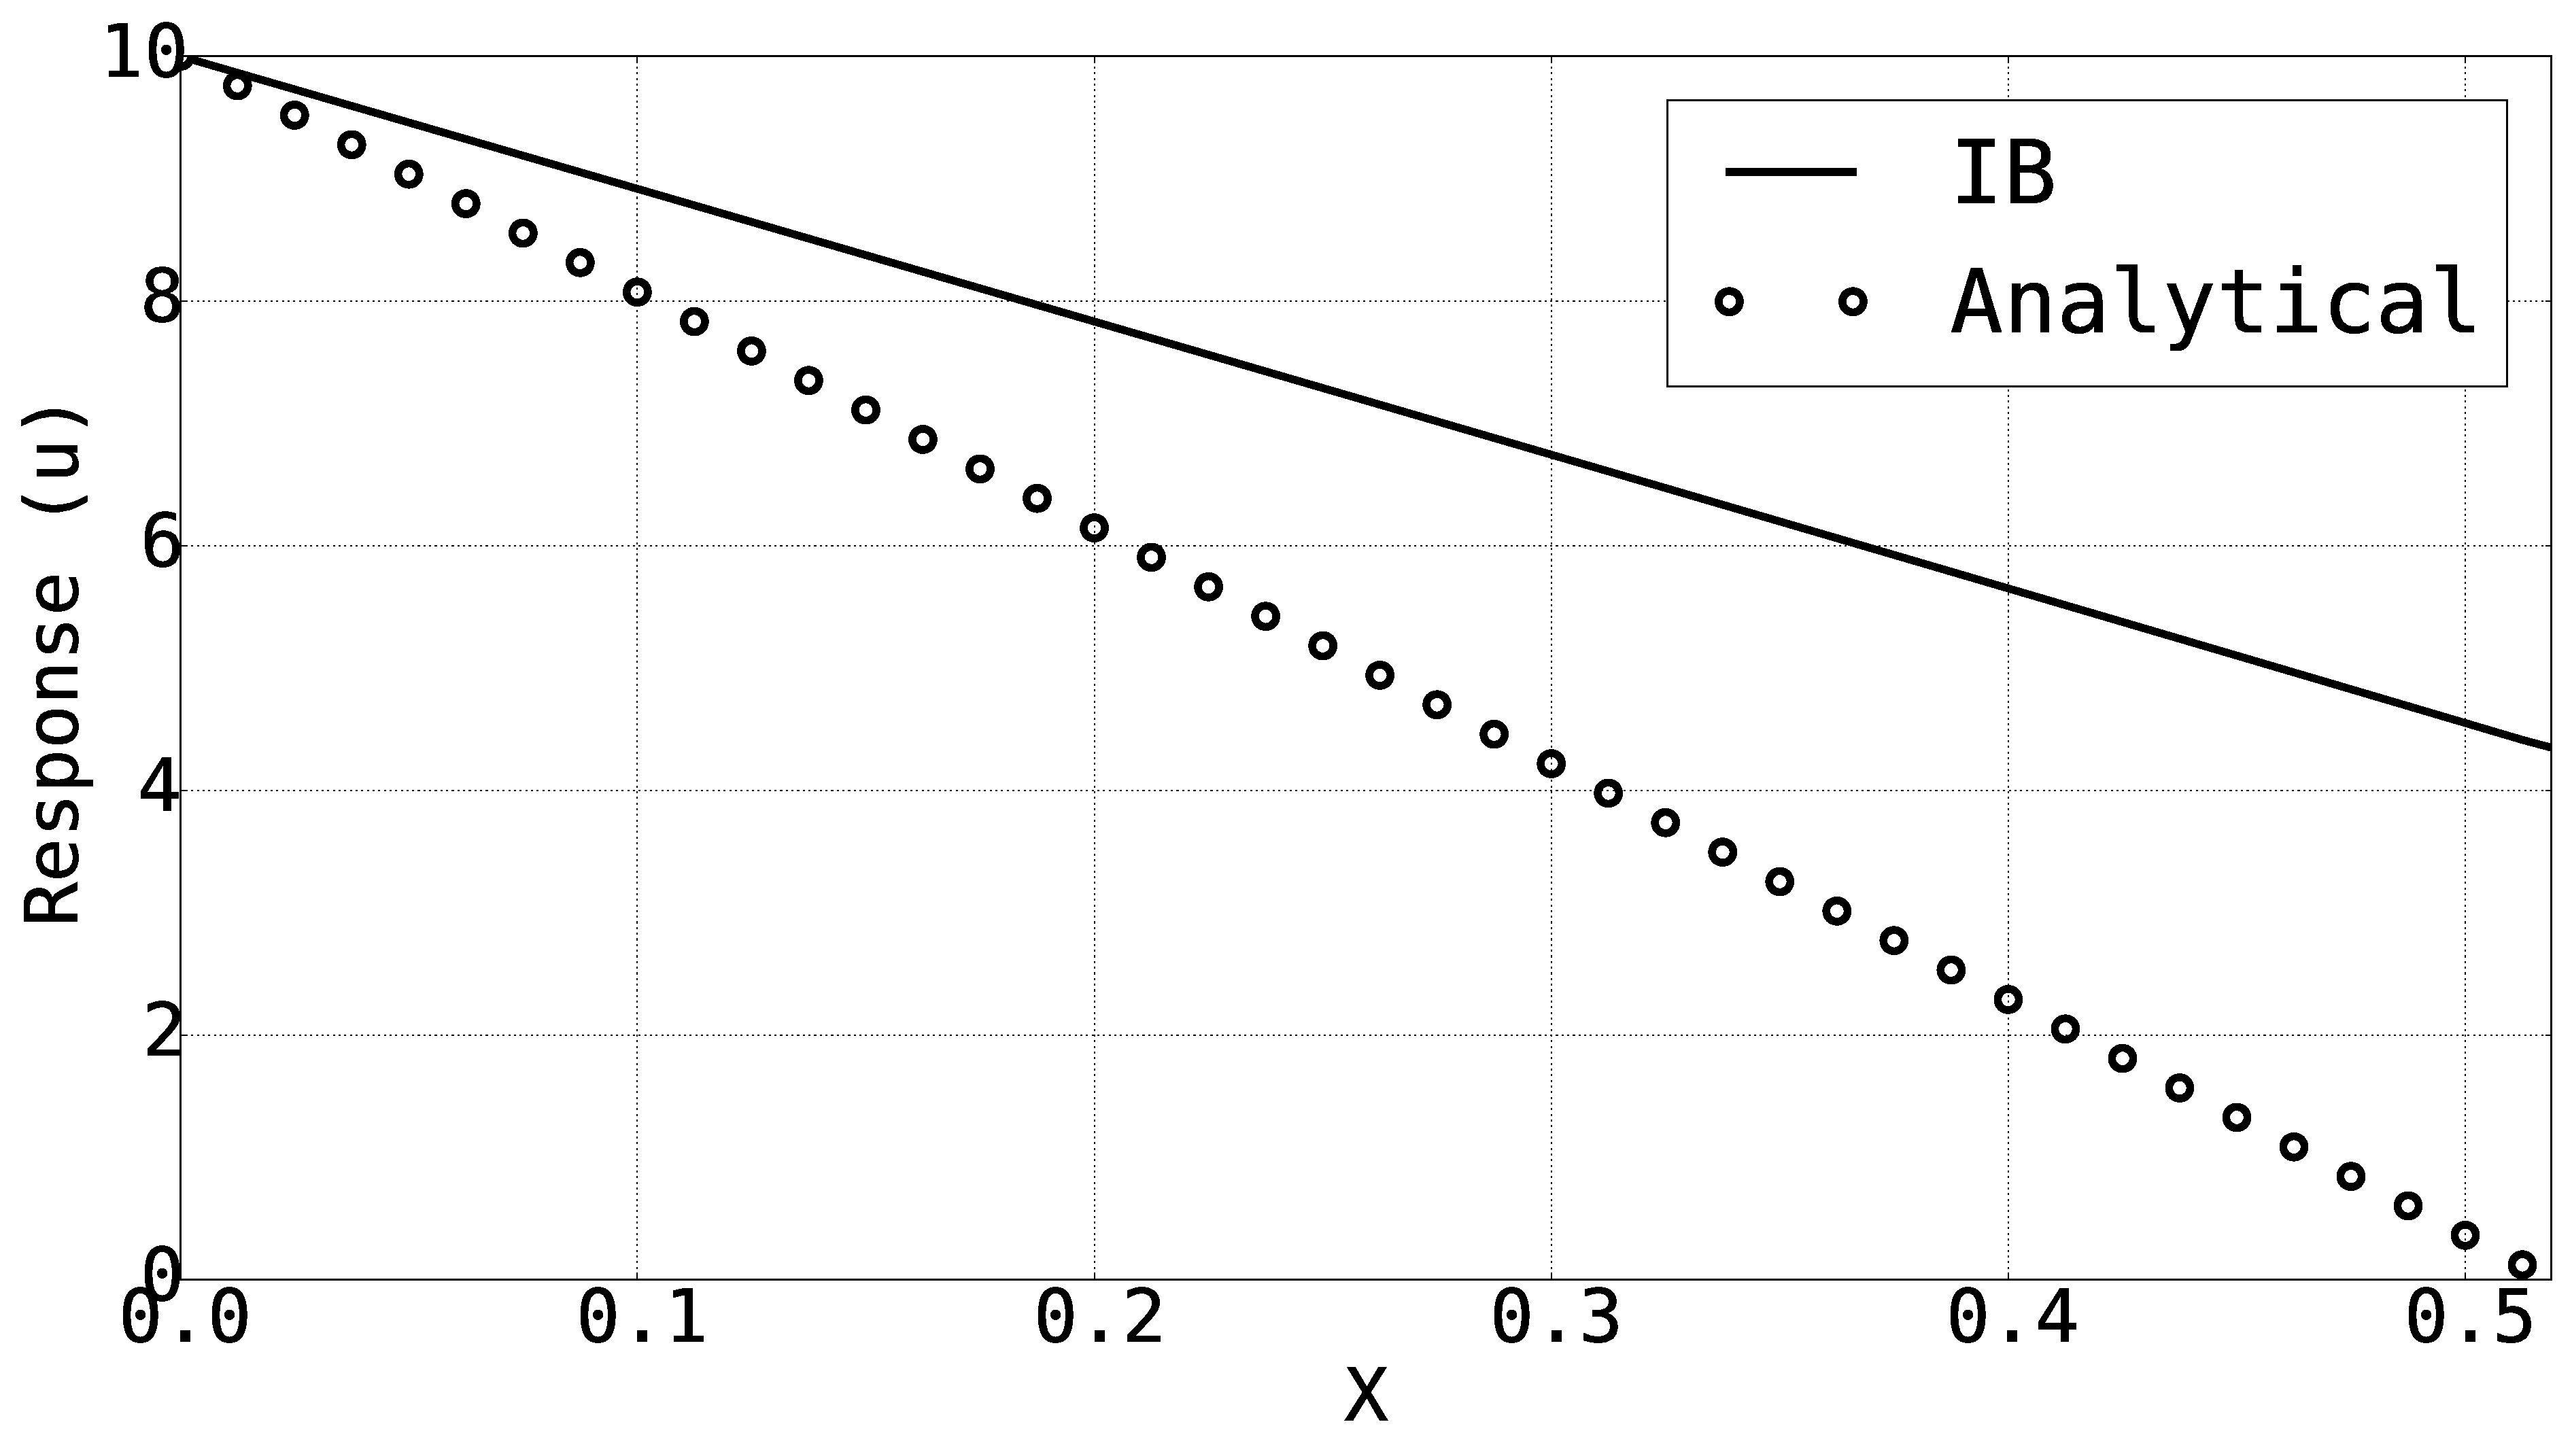
\includegraphics[width=7.0cm]{Chapter_3/figure/classicalIB_wallStiffness_2point_1.eps}
	}
	\\
	\subfigure[$K_{wall} = 10$]
	{
	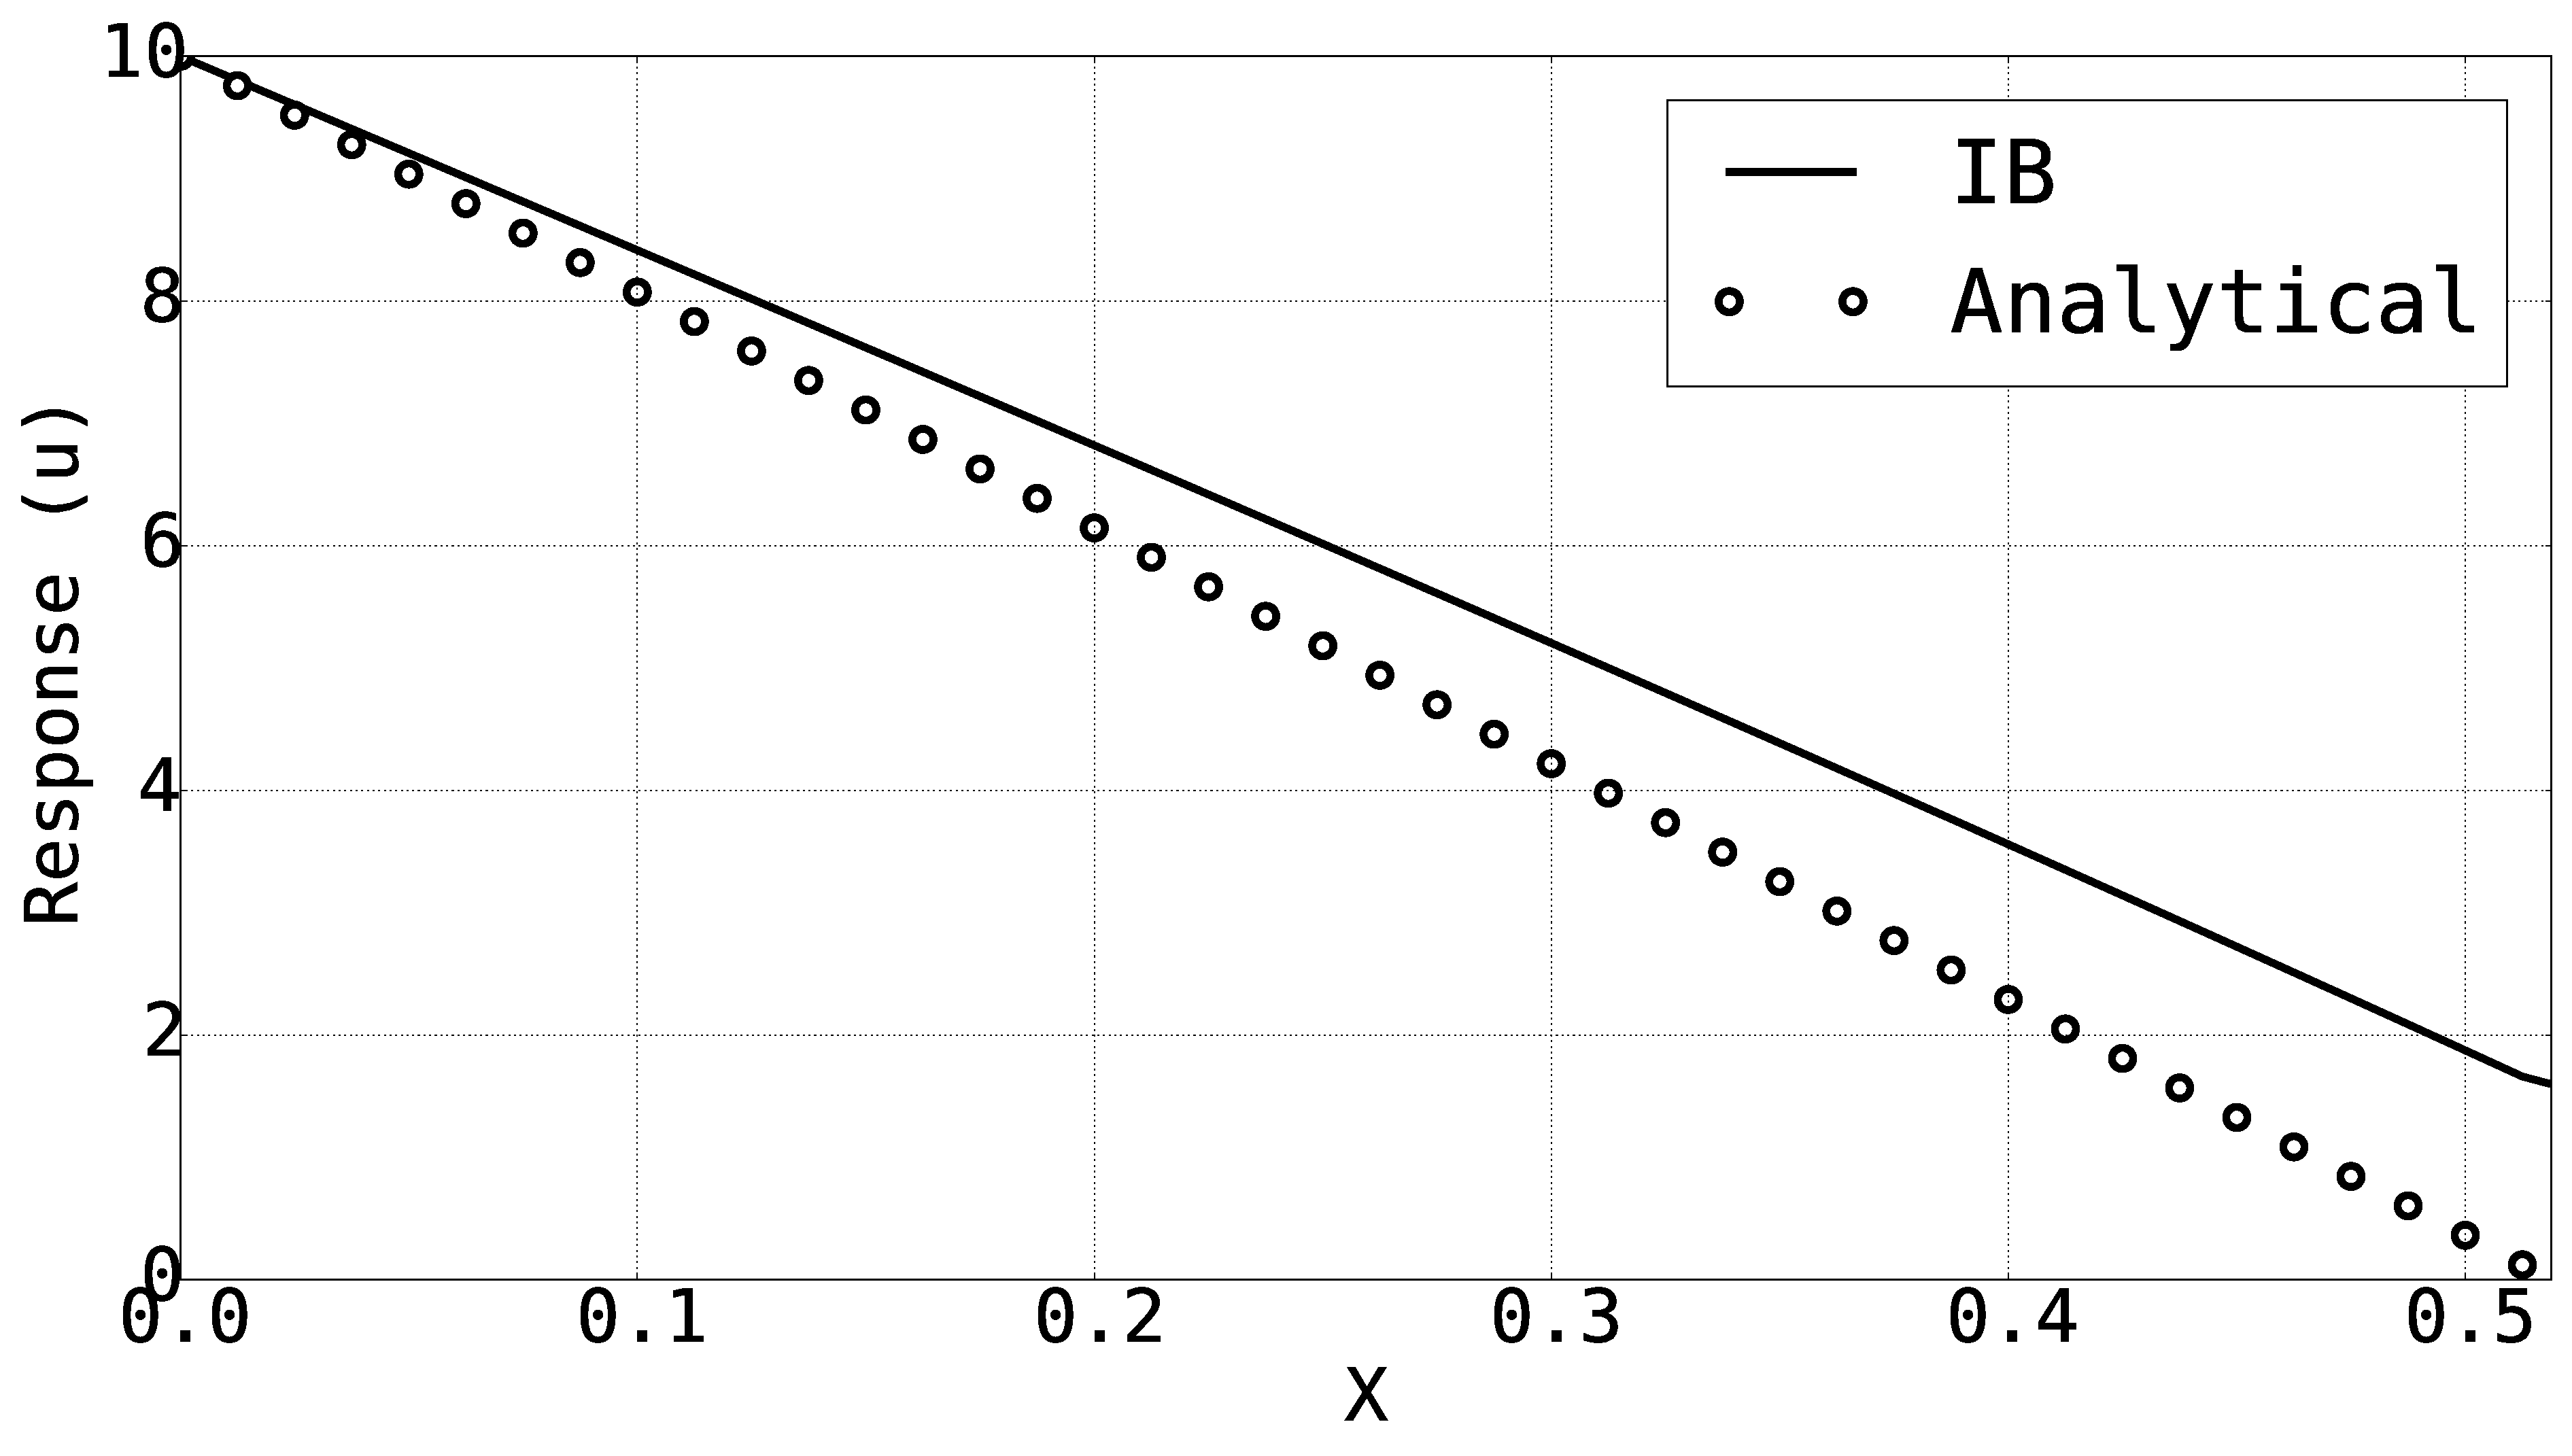
\includegraphics[width=7.0cm]{Chapter_3/figure/classicalIB_wallStiffness_2point_10.eps}
	}
	\quad
	\subfigure[$K_{wall} = 100$]
	{
	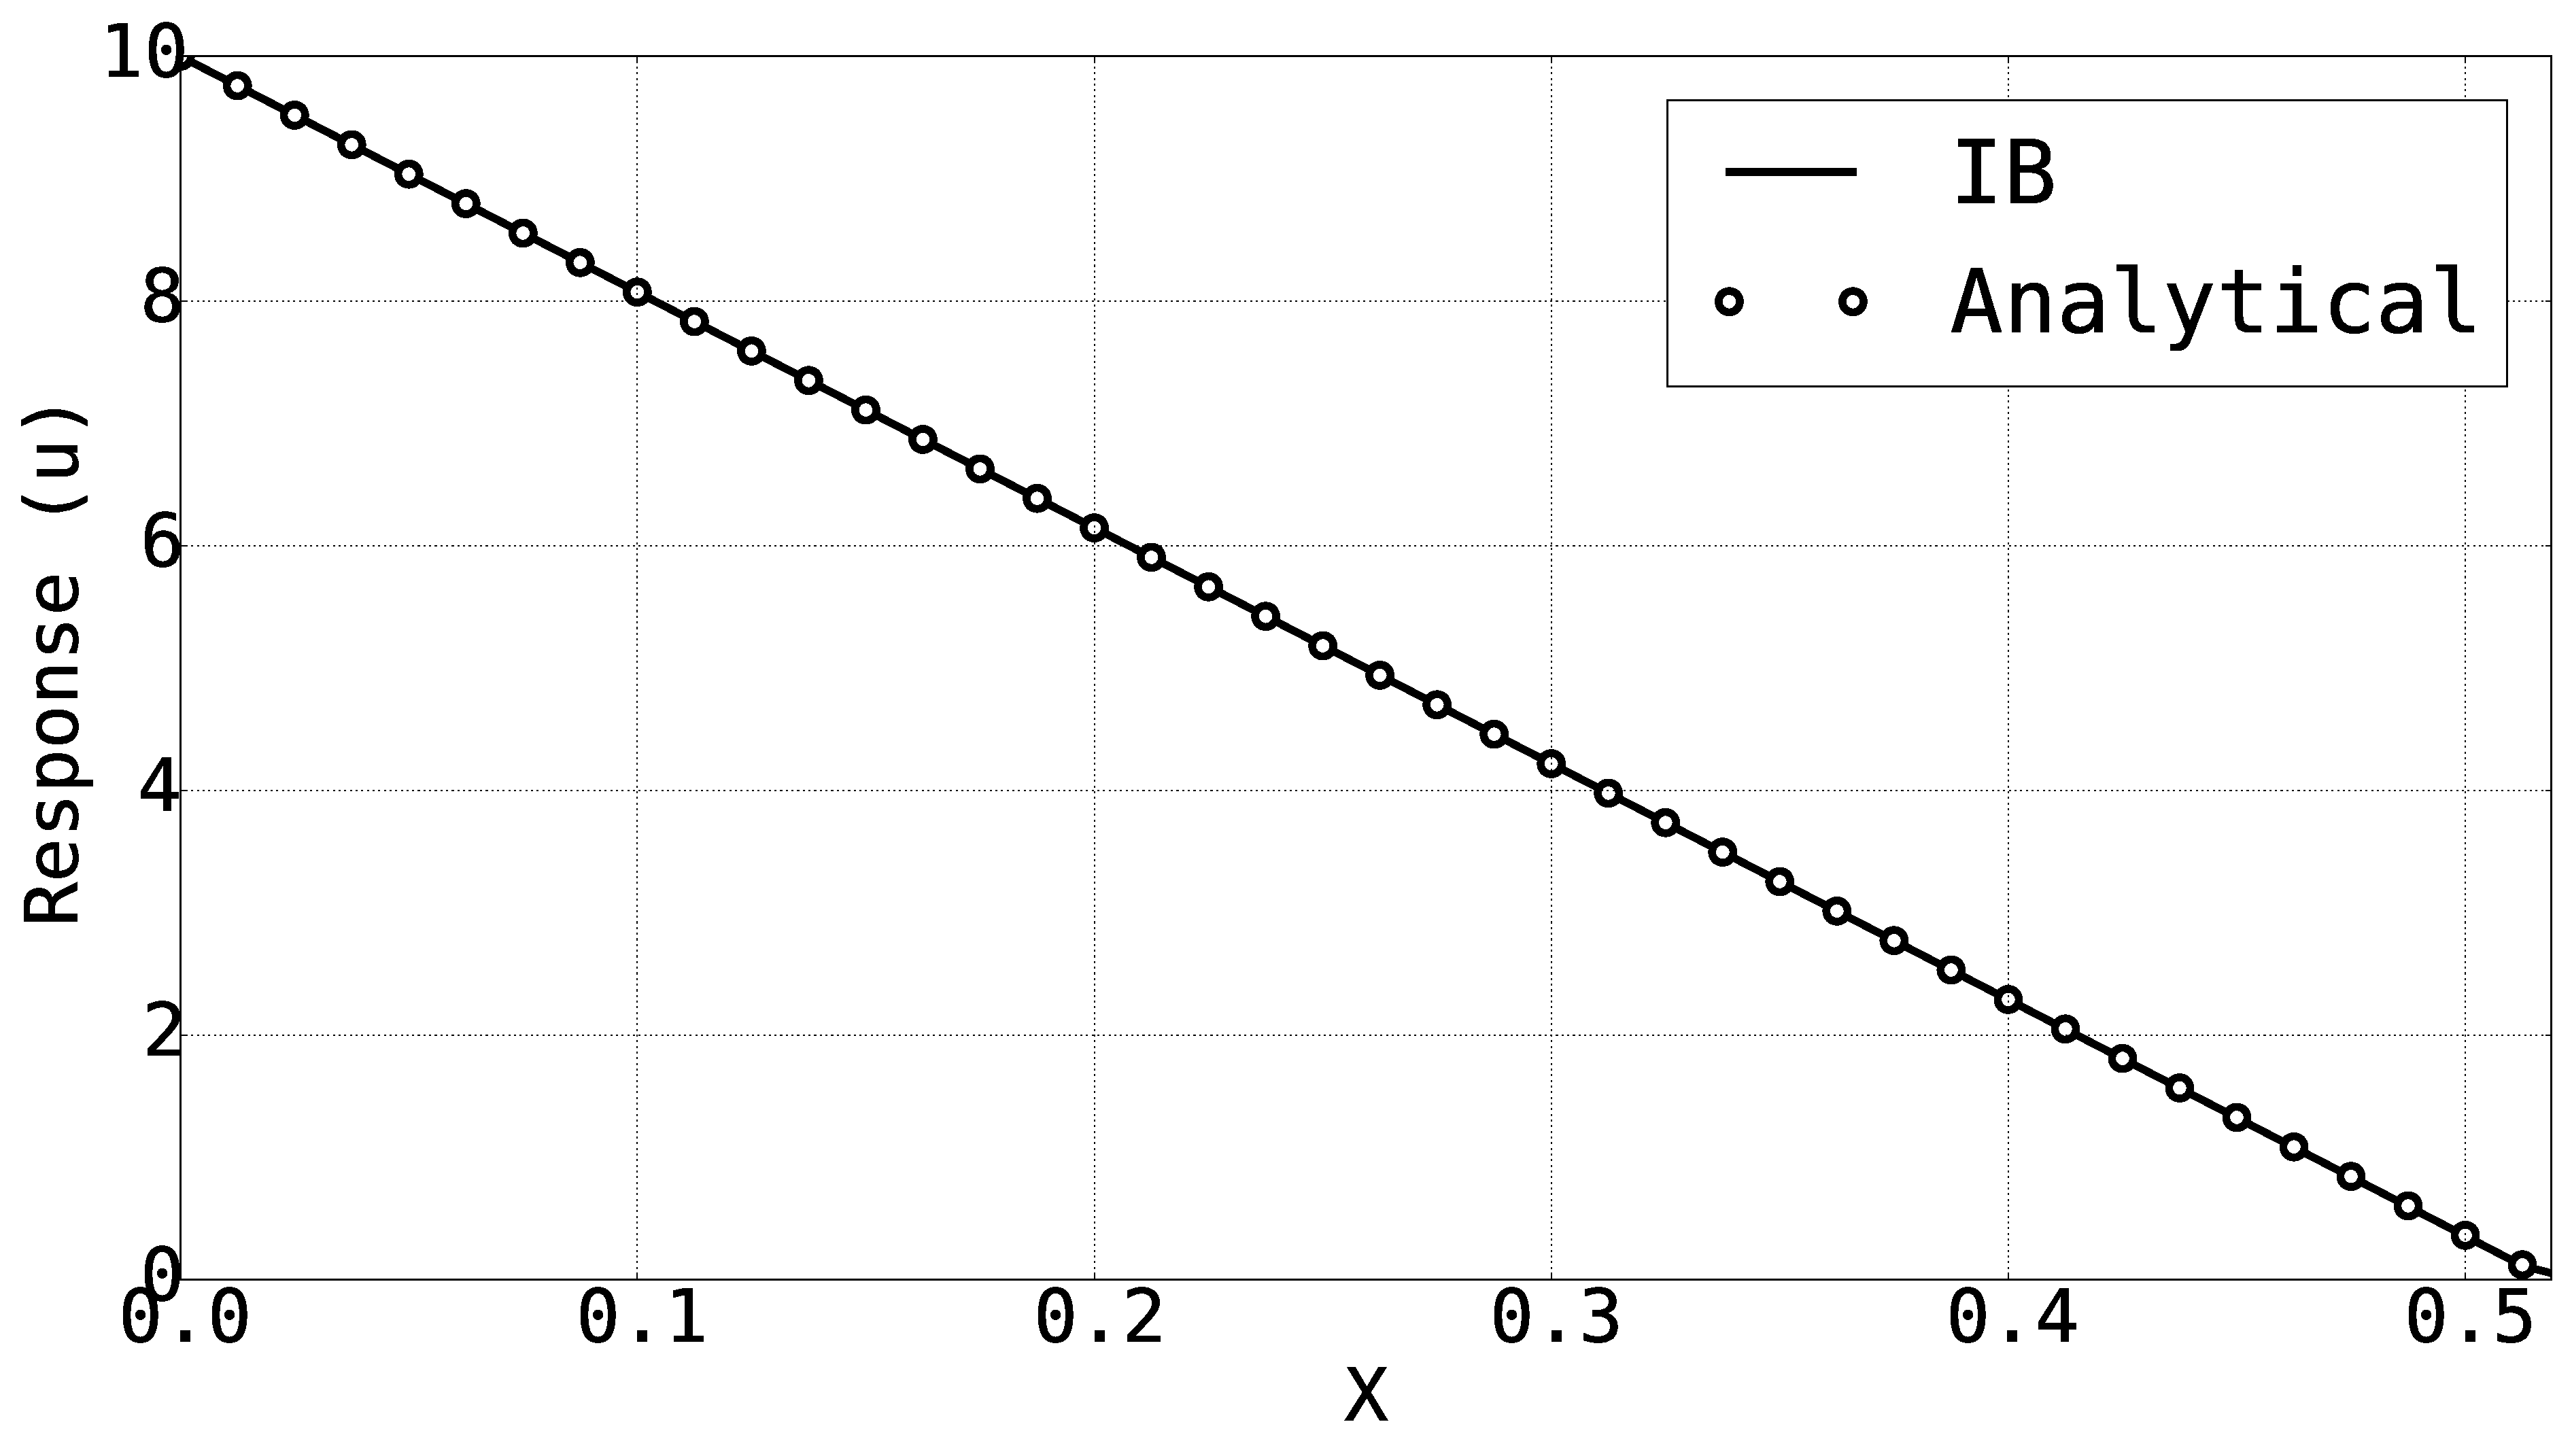
\includegraphics[width=7.0cm]{Chapter_3/figure/classicalIB_wallStiffness_2point_100.eps}
	}
	\caption{Comparison between IB and analytical results for different wall velocities.}
	\label{fig:C3_classicalIBResultWallStiffness}
\end{figure}

\begin{table}[H]
\centering
\begin{tabular}{c | c}
	 Wall velocity & RMSE \\ \hline \hline
	 0.1 & 0.1912 \\ \hline
	 1 & 0.1759  \\ \hline
	 10 & 0.0665 \\ \hline
	 100 & 0.001 \\
\end{tabular}
\caption{RMSE value for different wall stiffness values.}
\label{table:C3_classicalIBResultWallStiffnessRMSE}
\end{table}

% -.-.-.-.-.-.-.-.-.-.-.-.-.-.-.-.-.-.-.-.-.-.-.-.-.-.-.-.-.-.-.-.-.-
\subsection{Virtual boundary method}
The virtual boundary method is a different approach for imposing the effect of immersed boundary through force terms. This approach is well suited for both the rigid and elastic boundaries. The difference between this approach and the classical IB method is that it does not require the solution of the constitutive equations to calculate the force terms. This approach is based on the works of the works of Goldstein et al. \cite{goldstein1993modeling} to simulate the flow around the rigid bodies. The forcing term in the virtual boundary method is defined as

\begin{equation}\label{eq:C3_virtualBoundaryMethod}
	F(X_k, t) = 
	\alpha \int_0^t \left[ u(X_k, t) - U(X_k, t) \right] dt + 
	\beta \left[ u(X_k, t) - U(X_k, t) \right]
\end{equation}

where $F$ is the required force at the $k$-th Lagrangian point, $u(X_k, t)$ is the velocity calculated from the the Eulerian nodes using the $\delta$ function, and $U(X_k)$ is the desired velocity at the Lagrangian point $X_k$. The coefficient $\alpha$ and $\beta$ are selected to best enforce the boundary condition at the immersed solid boundary. Equation \eqref{eq:C3_virtualBoundaryMethod} is essentially a way to provide a feedback control to the system to make sure that the desired velocity ($U(X_k, t)$) is achieved at the immersed boundary. From a physical stand point, this equation represents a damped oscillator \cite{iaccarino2003immersed}.

As before, we apply this technique to the demonstration problem defined in Section \ref{sec:C3_benchmark_case}. We use the Crank-Nicholson method to discretize the equations as shown in the following equation. 

\begin{equation}\label{eq:C3_virtualBoundaryDiscretization}
	\frac{u^{n+1} - u^n}{\Delta t} = 
	\frac{1}{2}
	\left(
	\frac{\partial^2 u^{n+1}}{\partial x^2} +
	\frac{\partial^2 u^{n}}{\partial x^2}
	\right)
\end{equation}

where $n$ is the time step that we are at. The steps to solve this problem using the virtual boundary method can be defined as follows

\begin{enumerate}
	\item Define the initial condition as $u^0$ and set $f^0$ equal to zero.
	\item Calculate the velocity at the next time step, $u^1$, using Equation \eqref{eq:C3_discretizedEquationPeskinIB}
	\item Map the velocity results to the Lagrangian nodes using the $\delta$ function
	\item Based on the new velocity at $t=1$ evaluate Equation \eqref{eq:C3_virtualBoundaryMethod}.
	\item Map the force at the Lagrangian location $X$ to its neighbouring Eulerian points using $\delta$ function.
	\item Reiterate until the convergence is satisfied.
\end{enumerate}

Comparing the virtual boundary method to the classical IB method, we can see that less steps are required for this formulation. Moreover, there is no need to solve the constitutive equation for the solid domain which reduces the total computational cost.

Like the classical IB method, we investigate the effect of mesh size, moving wall velocity, and values for $\alpha$ and $\beta$ constants of the solution accuracy. The numerical results are verified with the analytical solution of this problem. We use the RMSE value as a metric to compare the results.

We looked at the effect of mesh size on the solution accuracy of the virtual boundary method. For this case, the moving wall velocity is fixed at $10 m/s$ with the location of fixed wall at $x_{wall} = 0.726$. The time step for this simulation is chosen as $10^{-5}$ with $\alpha = -1000$ and $\beta = -10$. We chose the node number as $11$, $41$, $81$, and $161$. The total length of the domain is chosen as $1 m$. As shown in Figure \ref{C3_virtualBoundaryResultNodeNumber} and Table \ref{table:C3_virtualBoundaryResultNodeNumberRMSE}, by increasing the nodes number the simulation results become more accurate. However, the convergence is reached earlier compared to the classical IB method of last section. This means that the computational effort to get the same accuracy compared to classical IB method is much less when using the virtual boundary method. 

\begin{figure}[H]
	\centering
	\subfigure[N = 11]
	{
	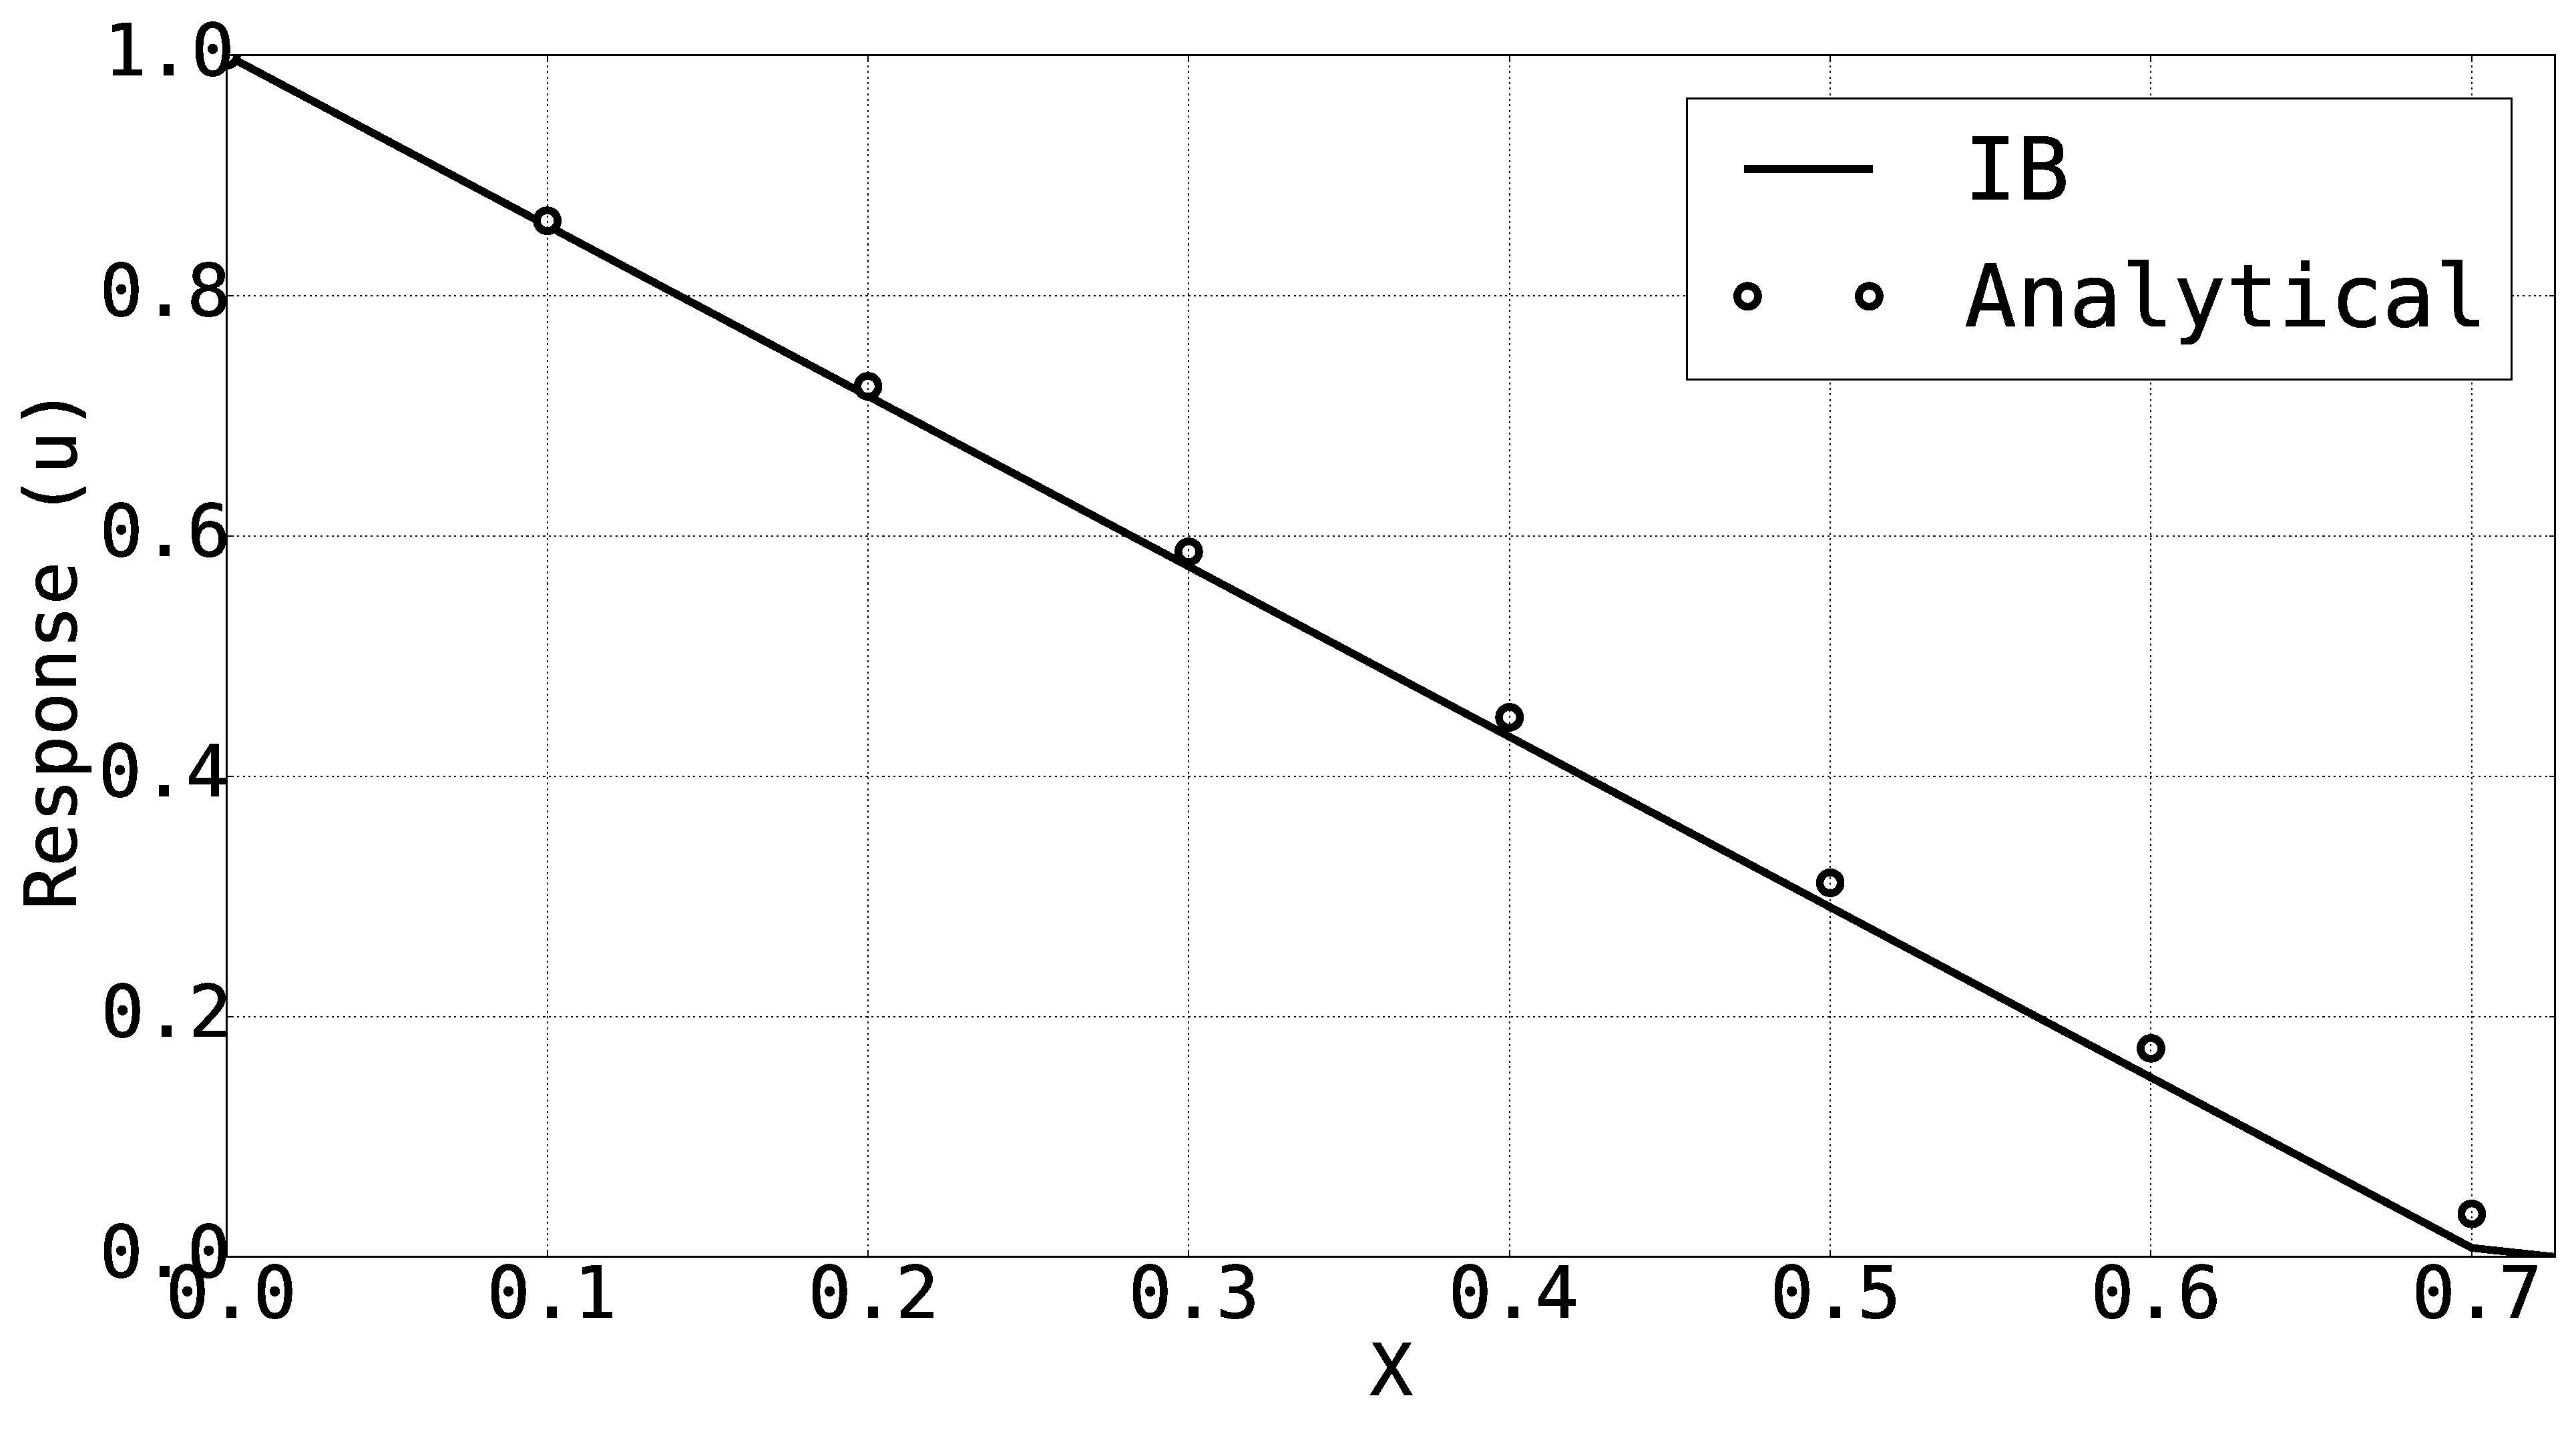
\includegraphics[width=7.0cm]{Chapter_3/figure/virtualBoundary_nodeNumber_11.eps}
	}
	\quad
	\subfigure[N = 41]
	{
	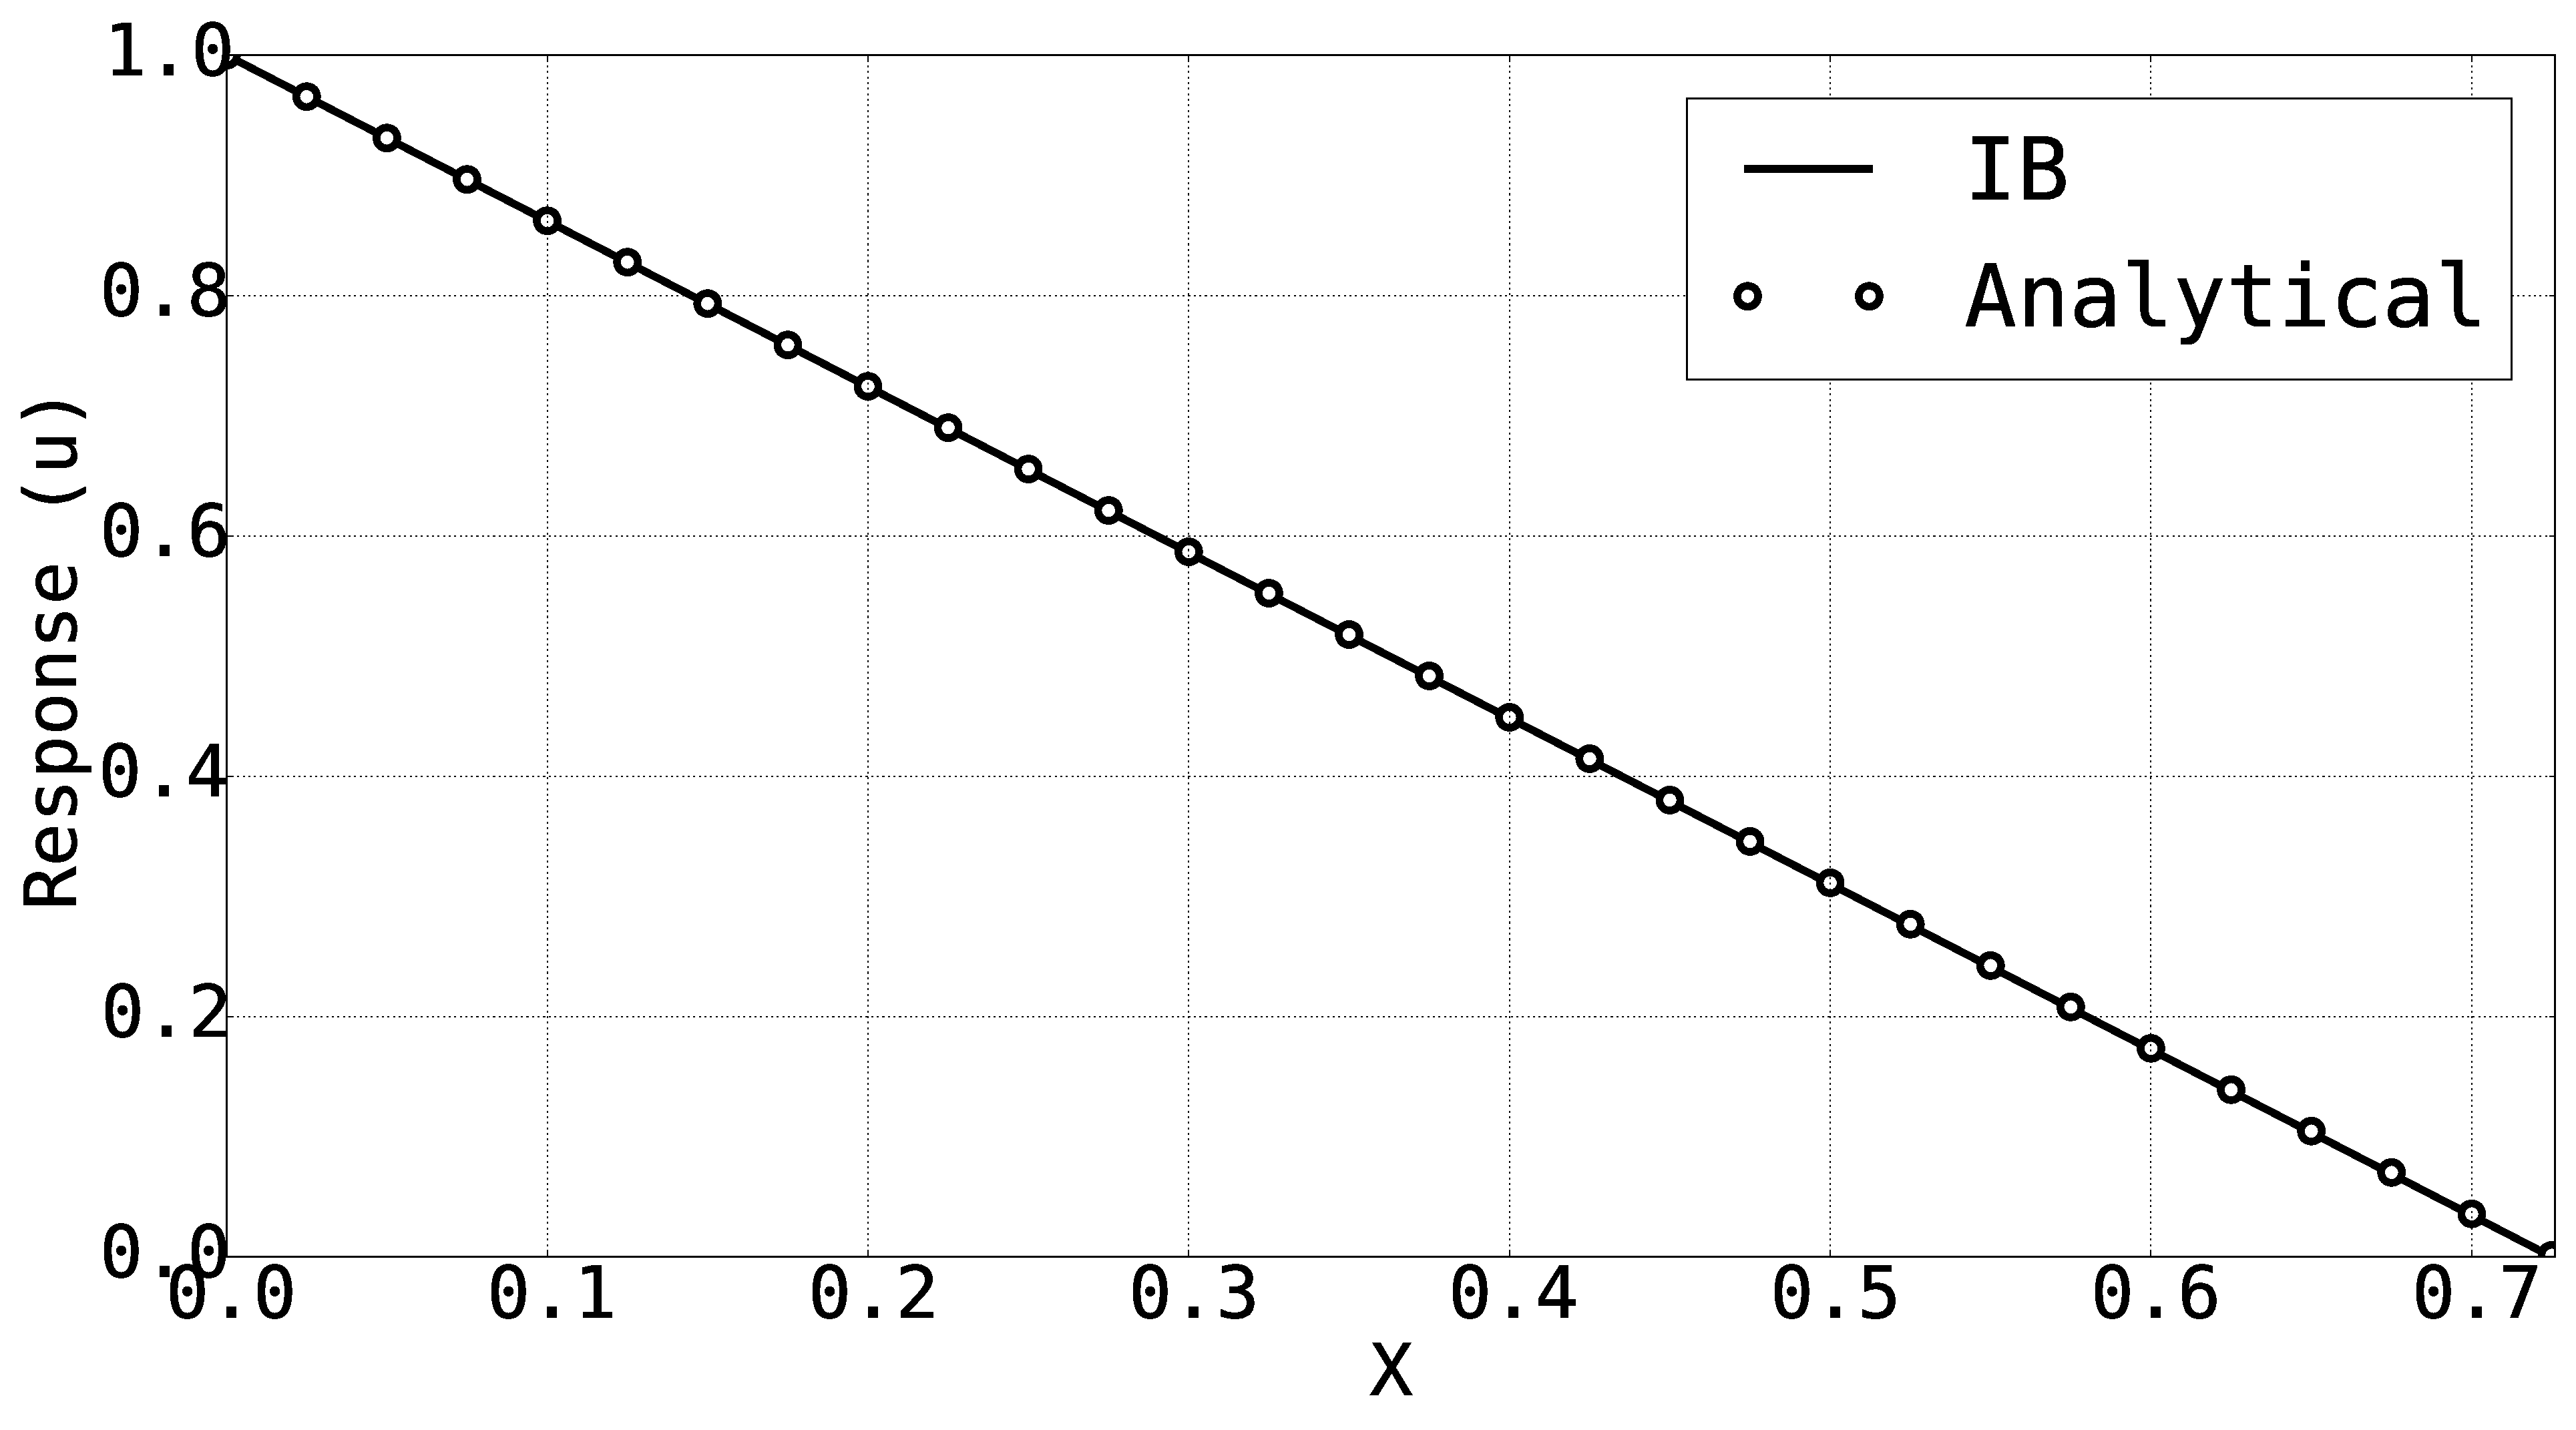
\includegraphics[width=7.0cm]{Chapter_3/figure/virtualBoundary_nodeNumber_41.eps}
	}
	\\
	\subfigure[N = 81]
	{
	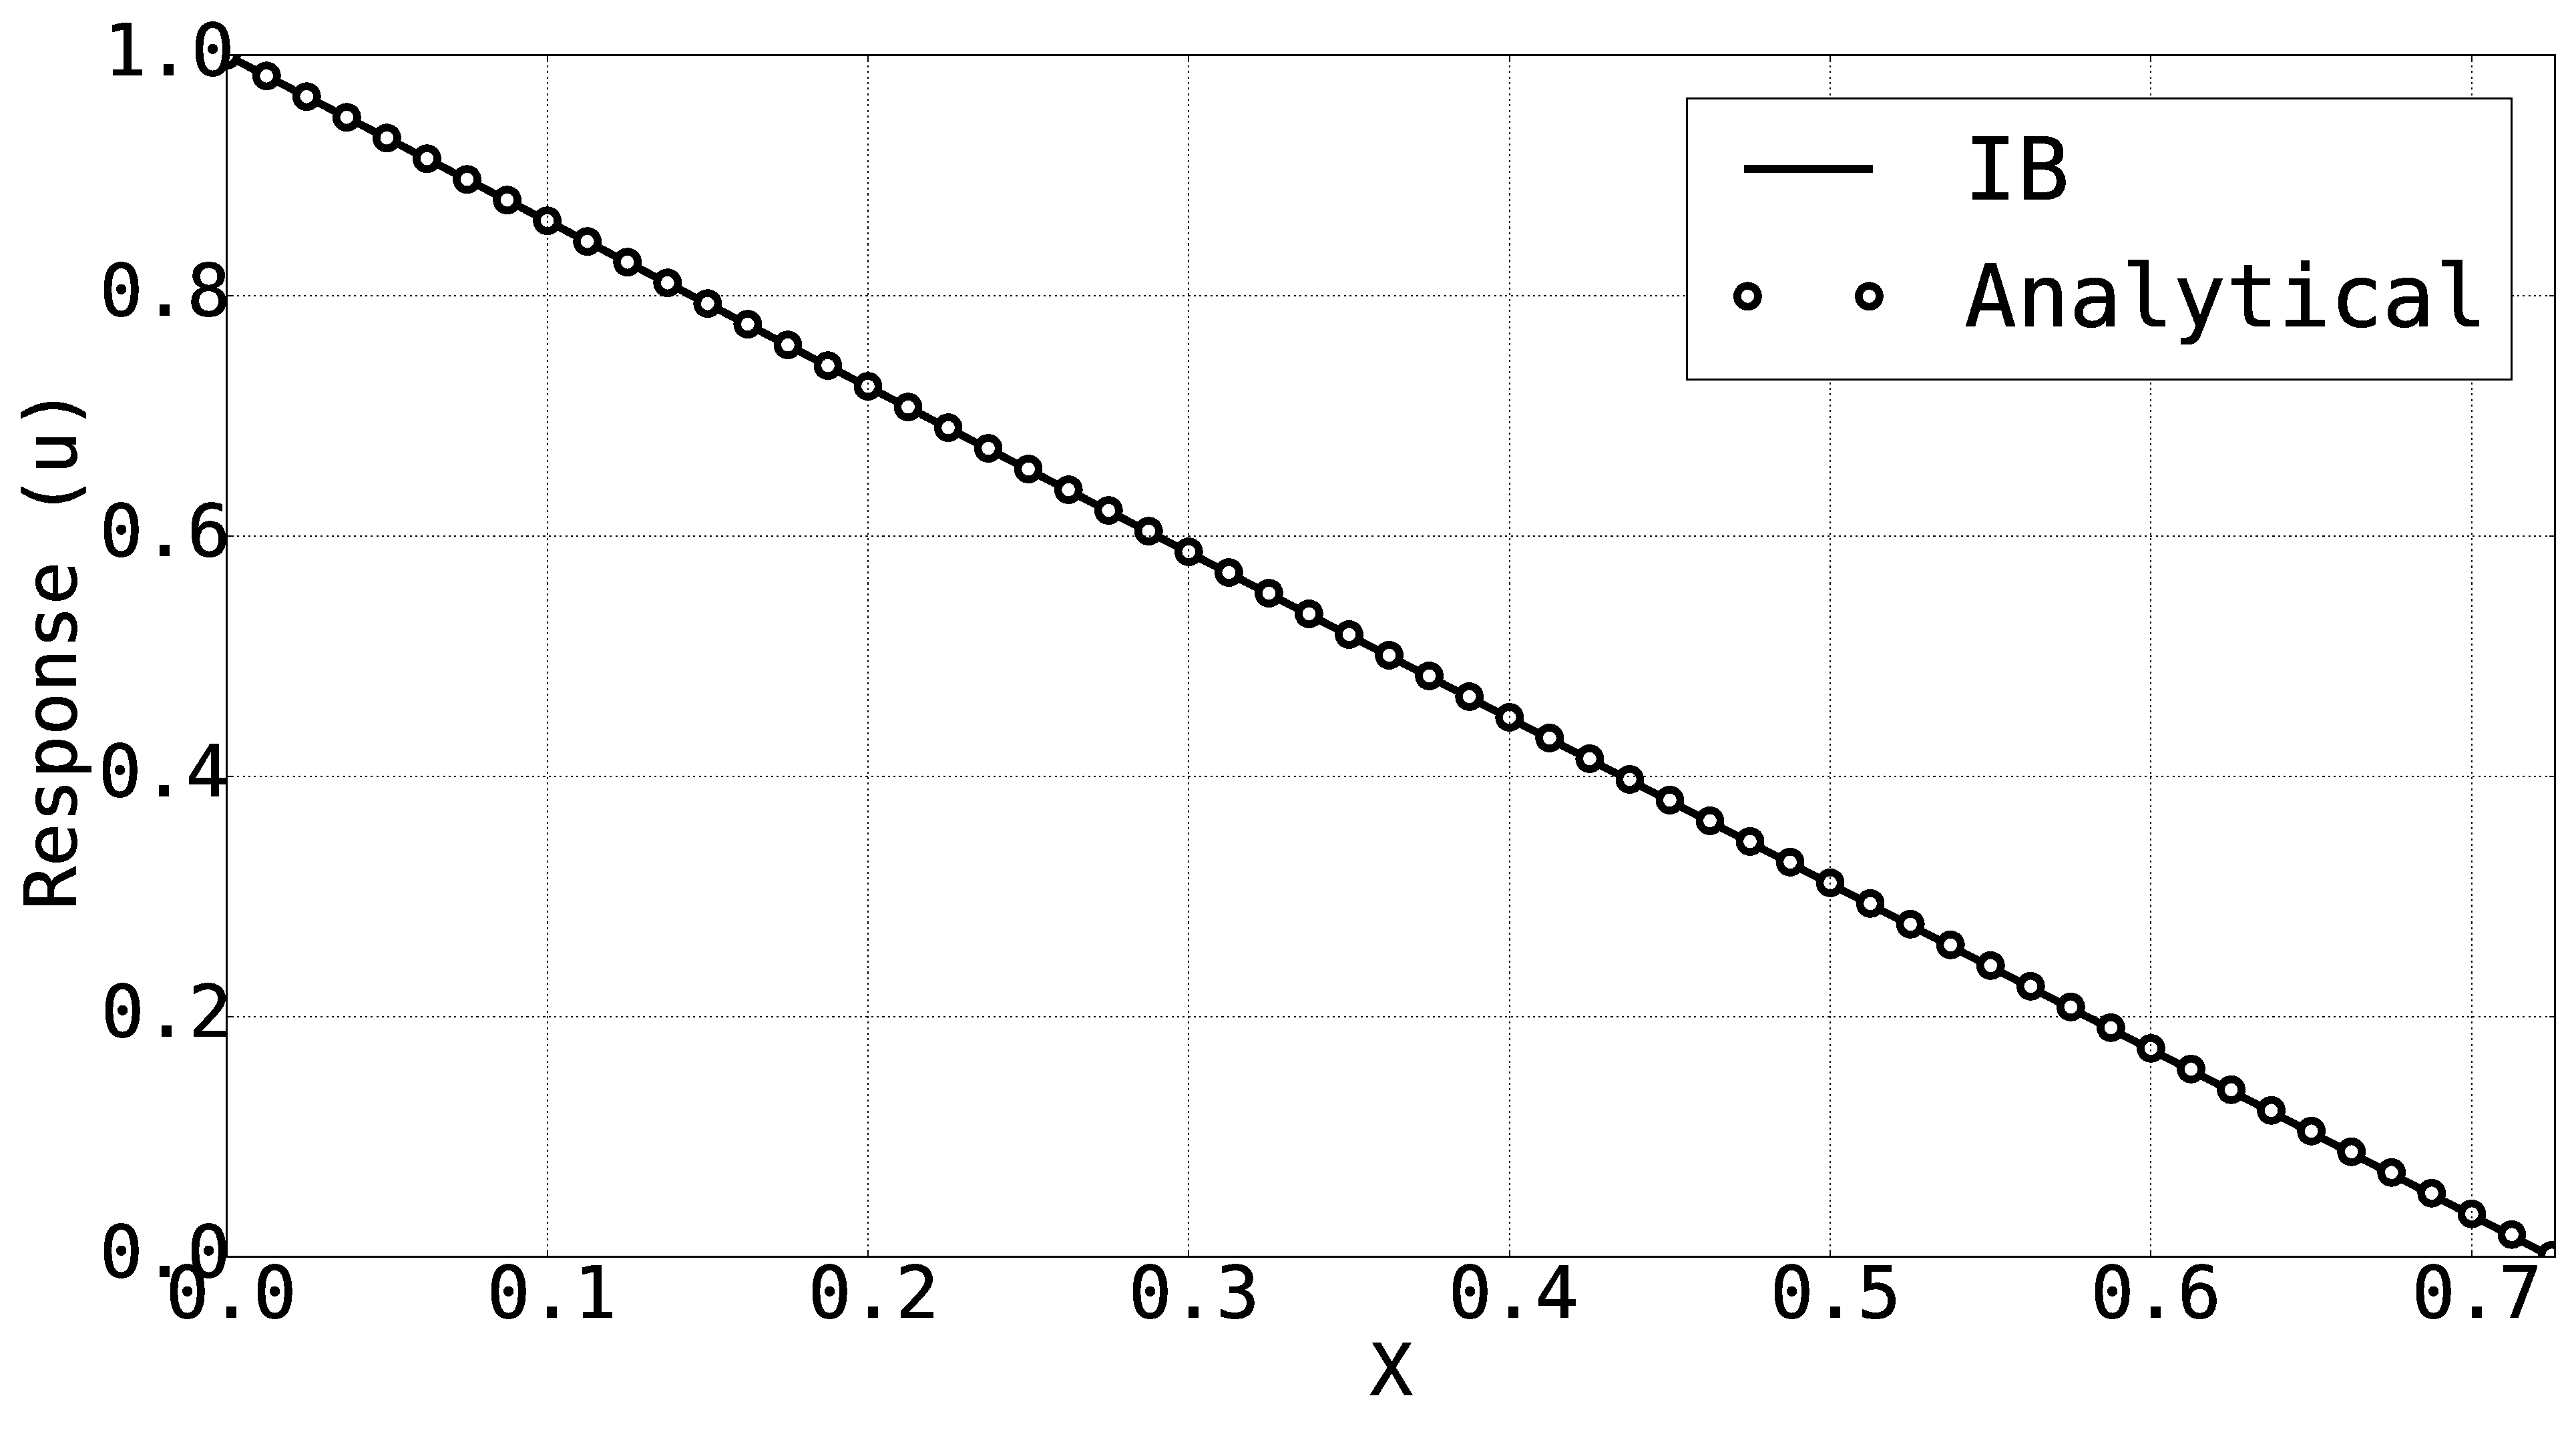
\includegraphics[width=7.0cm]{Chapter_3/figure/virtualBoundary_nodeNumber_81.eps}
	}
	\quad
	\subfigure[N = 161]
	{
	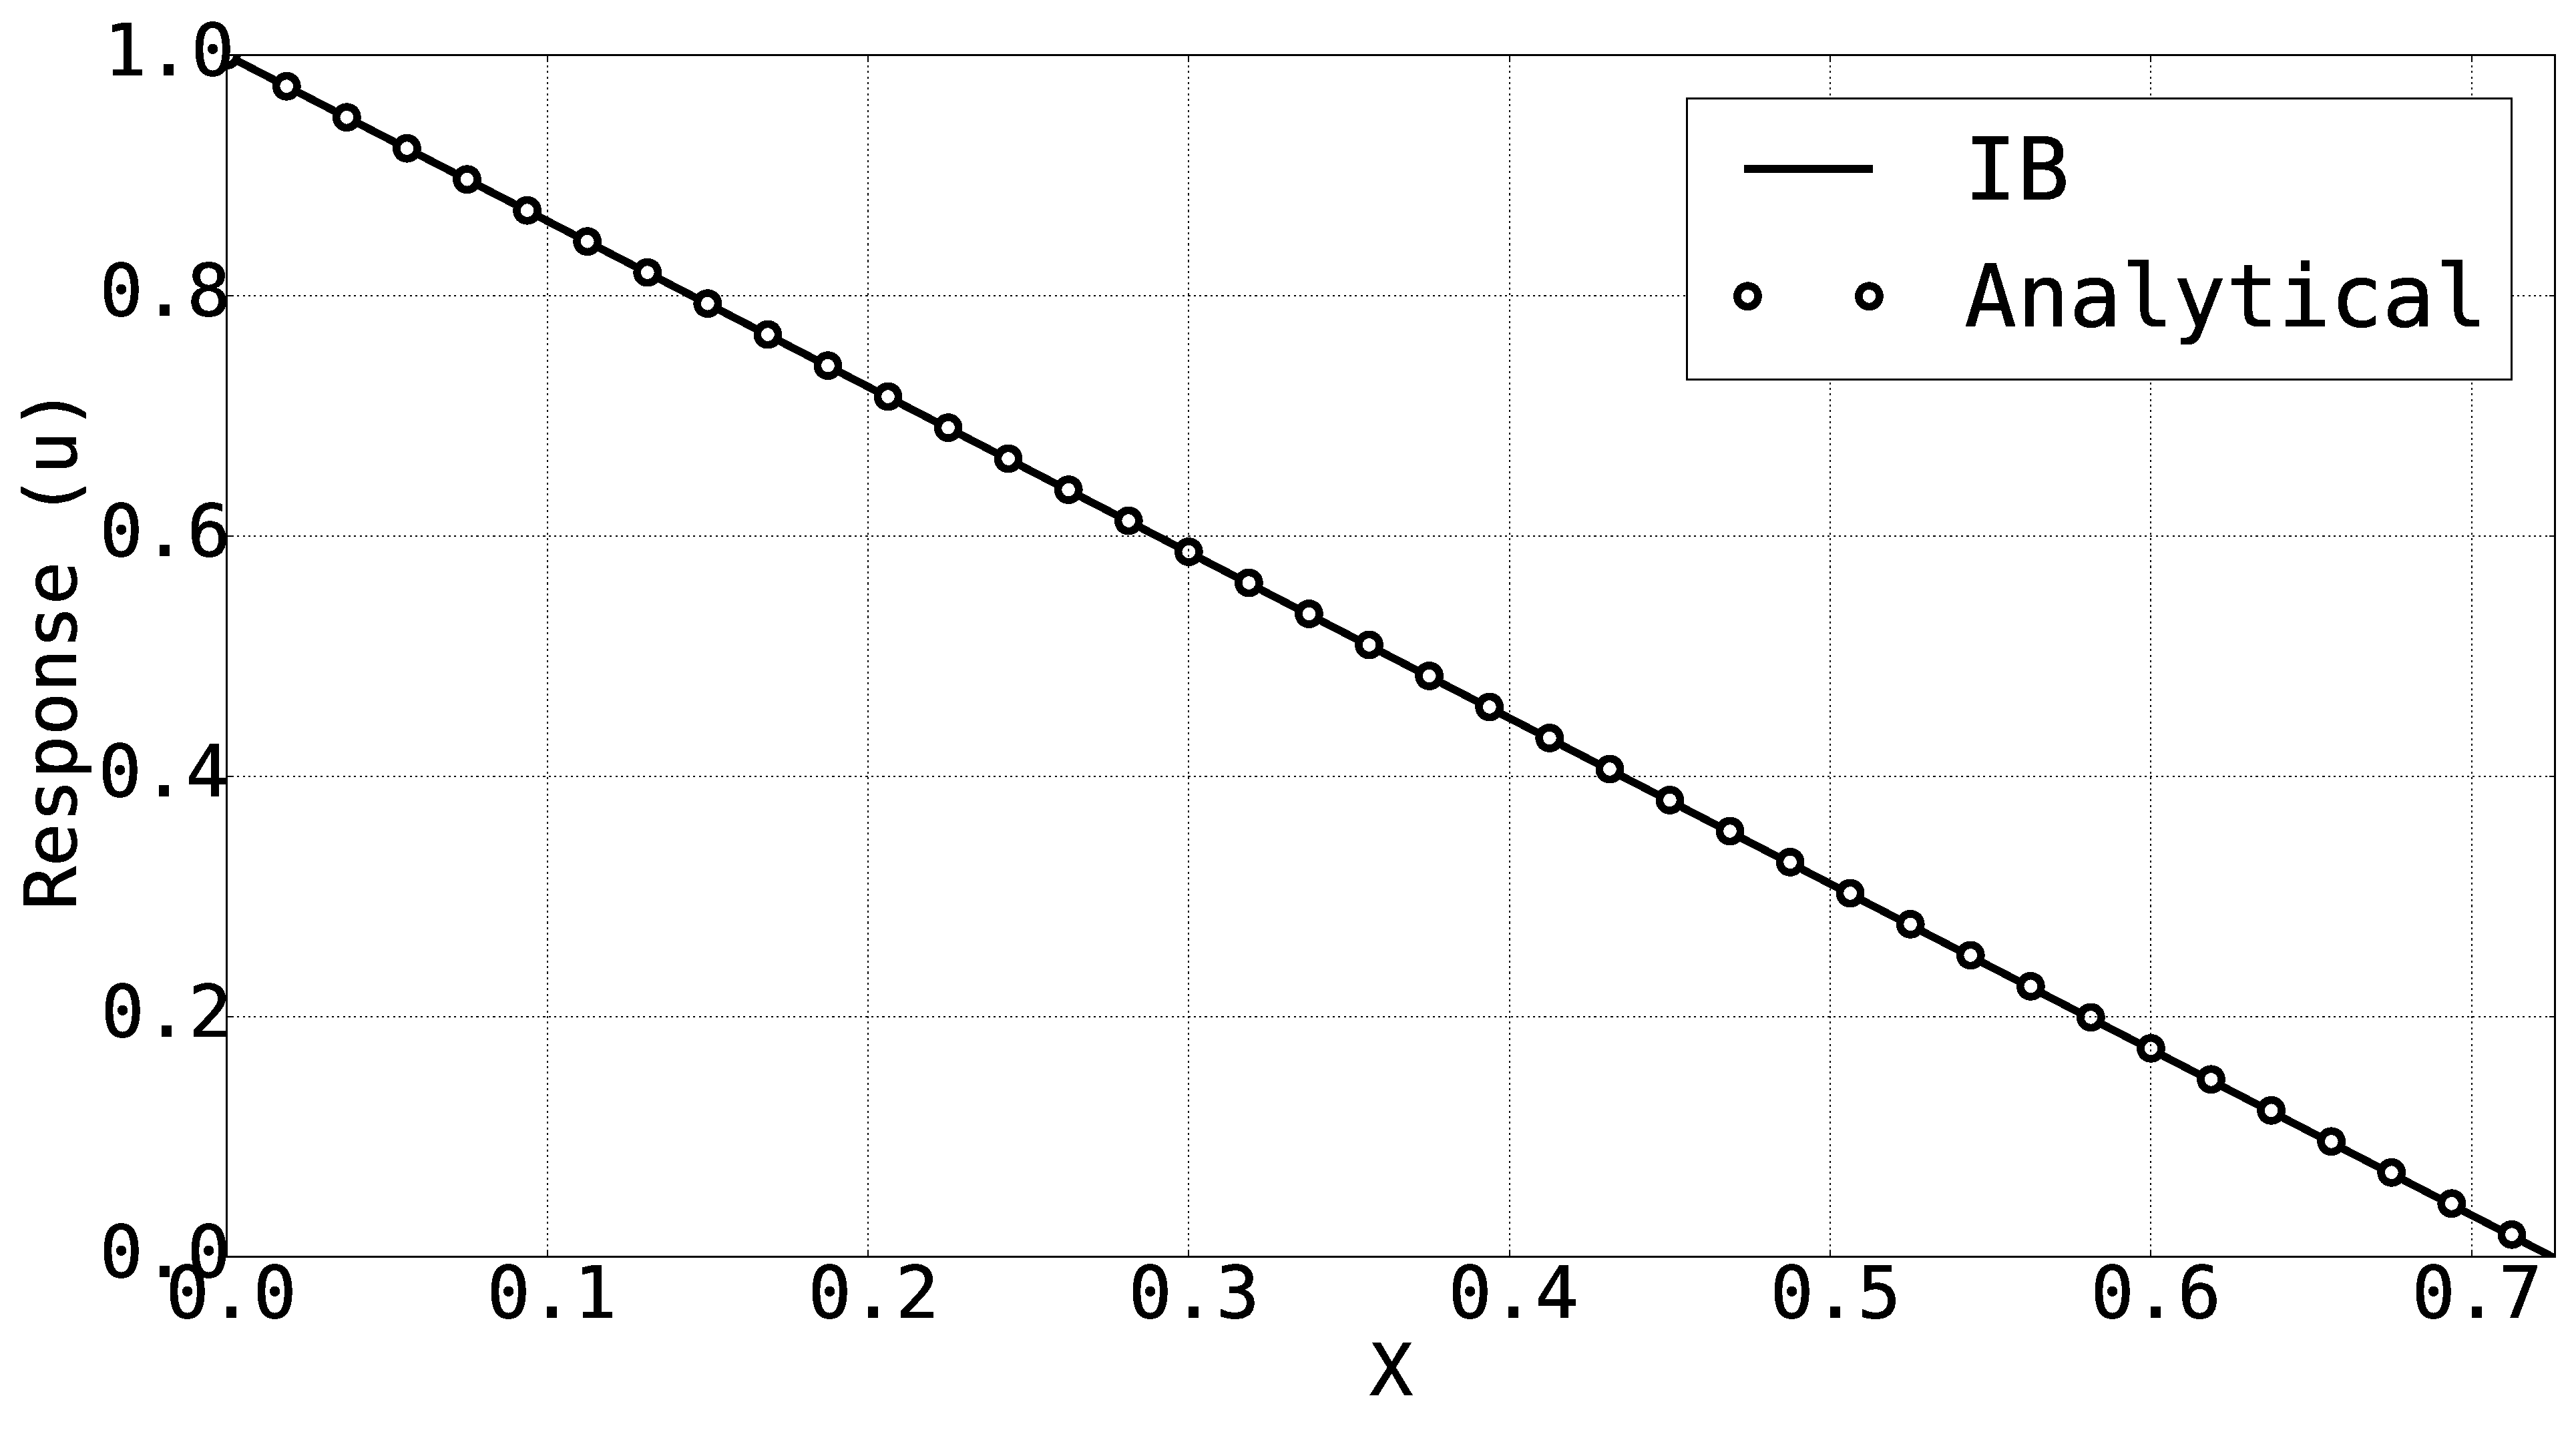
\includegraphics[width=7.0cm]{Chapter_3/figure/virtualBoundary_nodeNumber_161.eps}
	}
	\caption{Comparison between IB and analytical results for different porosity values.}
	\label{fig:C3_virtualBoundaryResultNodeNumber}
\end{figure}

\begin{table}[H]
\centering
\begin{tabular}{c | c }
	 Node number & RMSE \\ \hline \hline
	 11 & 0.012 \\ \hline
	 41 & 0.00065 \\ \hline
	 81 & 0.00063 \\ \hline
	 161 & 0.00058 \\
\end{tabular}
\caption{RMSE value for different node numbers.}
\label{table:C3_virtualBoundaryResultNodeNumberRMSE}
\end{table}

We looked at the effect of wall velocity of the solution accuracy. As before the length of the domain is fixed at $1 m$ with wall defined at $x_{wall} = 0.726$, the time step is chosen as $10^{-5}$. We chose the $\alpha$ and $\beta$ constants as $-1000$ and $-10$ respectively. We simulated the flow selecting the wall velocity as $10$, $100$, $1000$, and $10000$. The results are compared with the analytical results. As shown in Figure \ref{fig:C3_virtualBoundaryResultWallVelocity} and Table \ref{table:C3_virtualBoundaryResultWallVelocityRMSE}, the wall velocity does not affect the accuracy of the solution. When compared with the results of the classical IB method in previous section, we can see that the virtual boundary method produces more accurate results. Moreover, the simulation time is much less than the classical IB method.

\begin{figure}[H]
	\centering
	\subfigure[$u_{wall} = 10 m/s$]
	{
	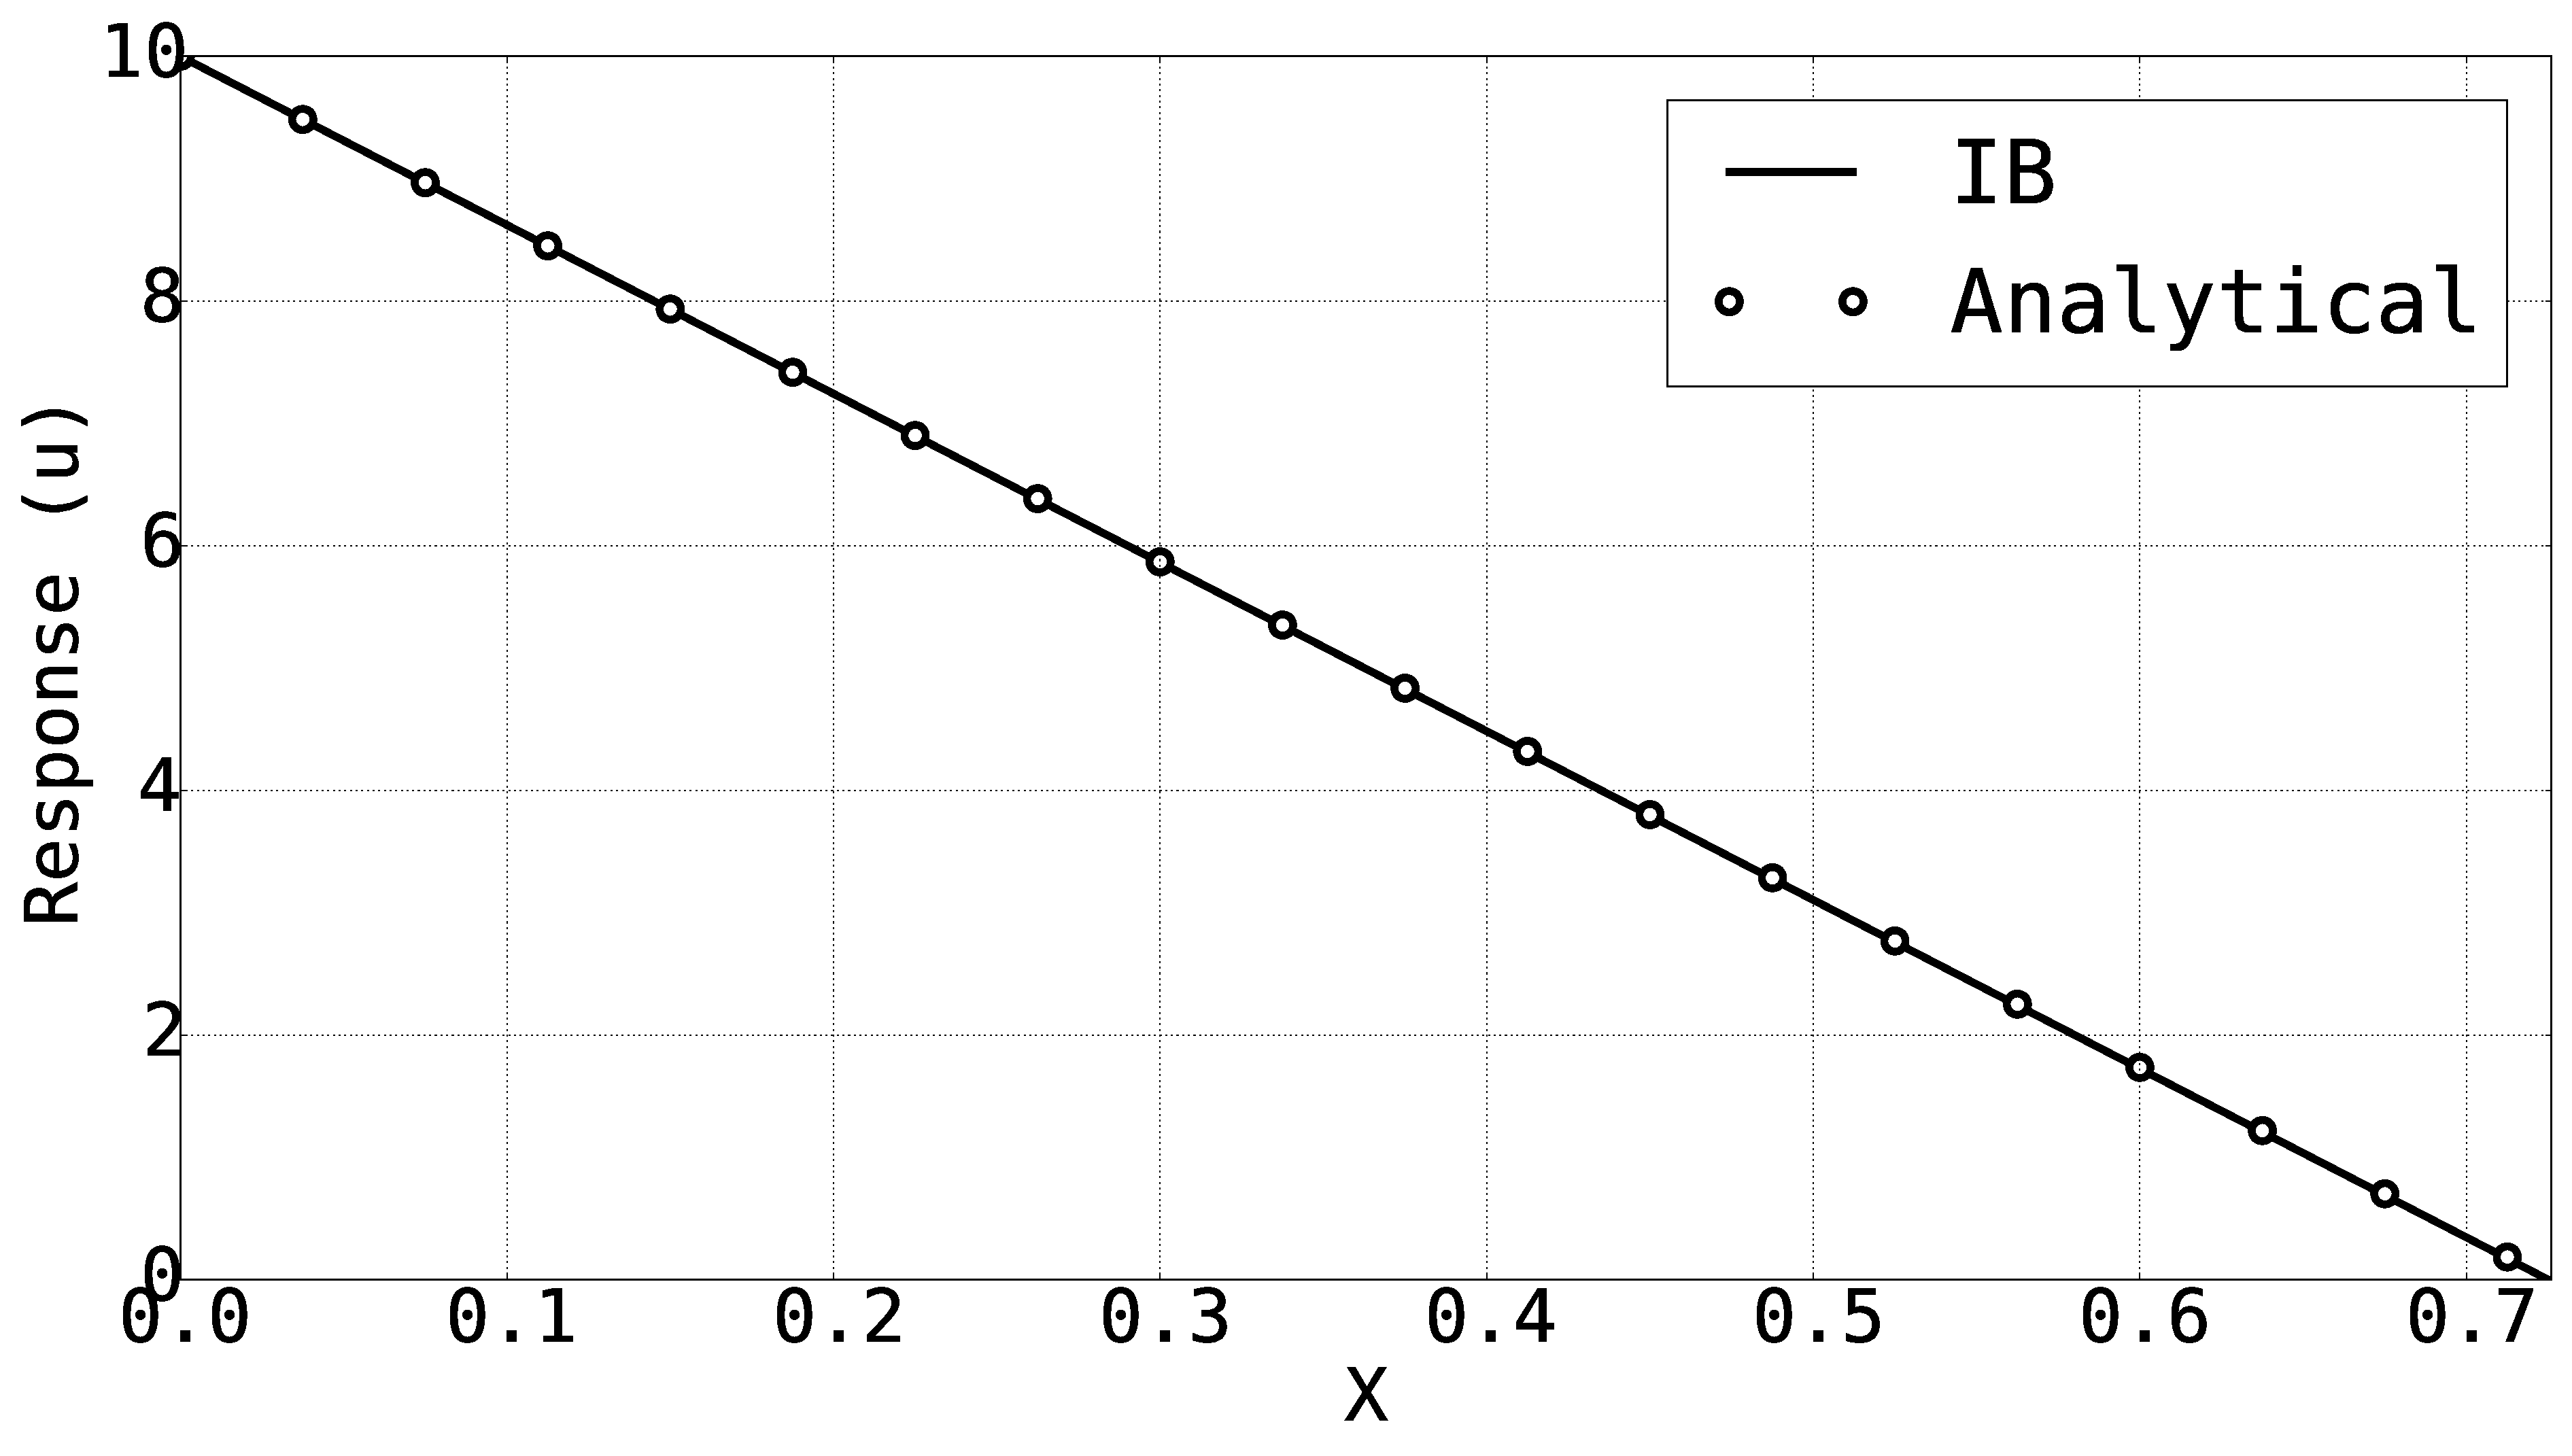
\includegraphics[width=7.0cm]{Chapter_3/figure/virtualBoundary_wallVelocity_10.eps}
	}
	\quad
	\subfigure[$u_{wall} = 10^2 m/s$]
	{
	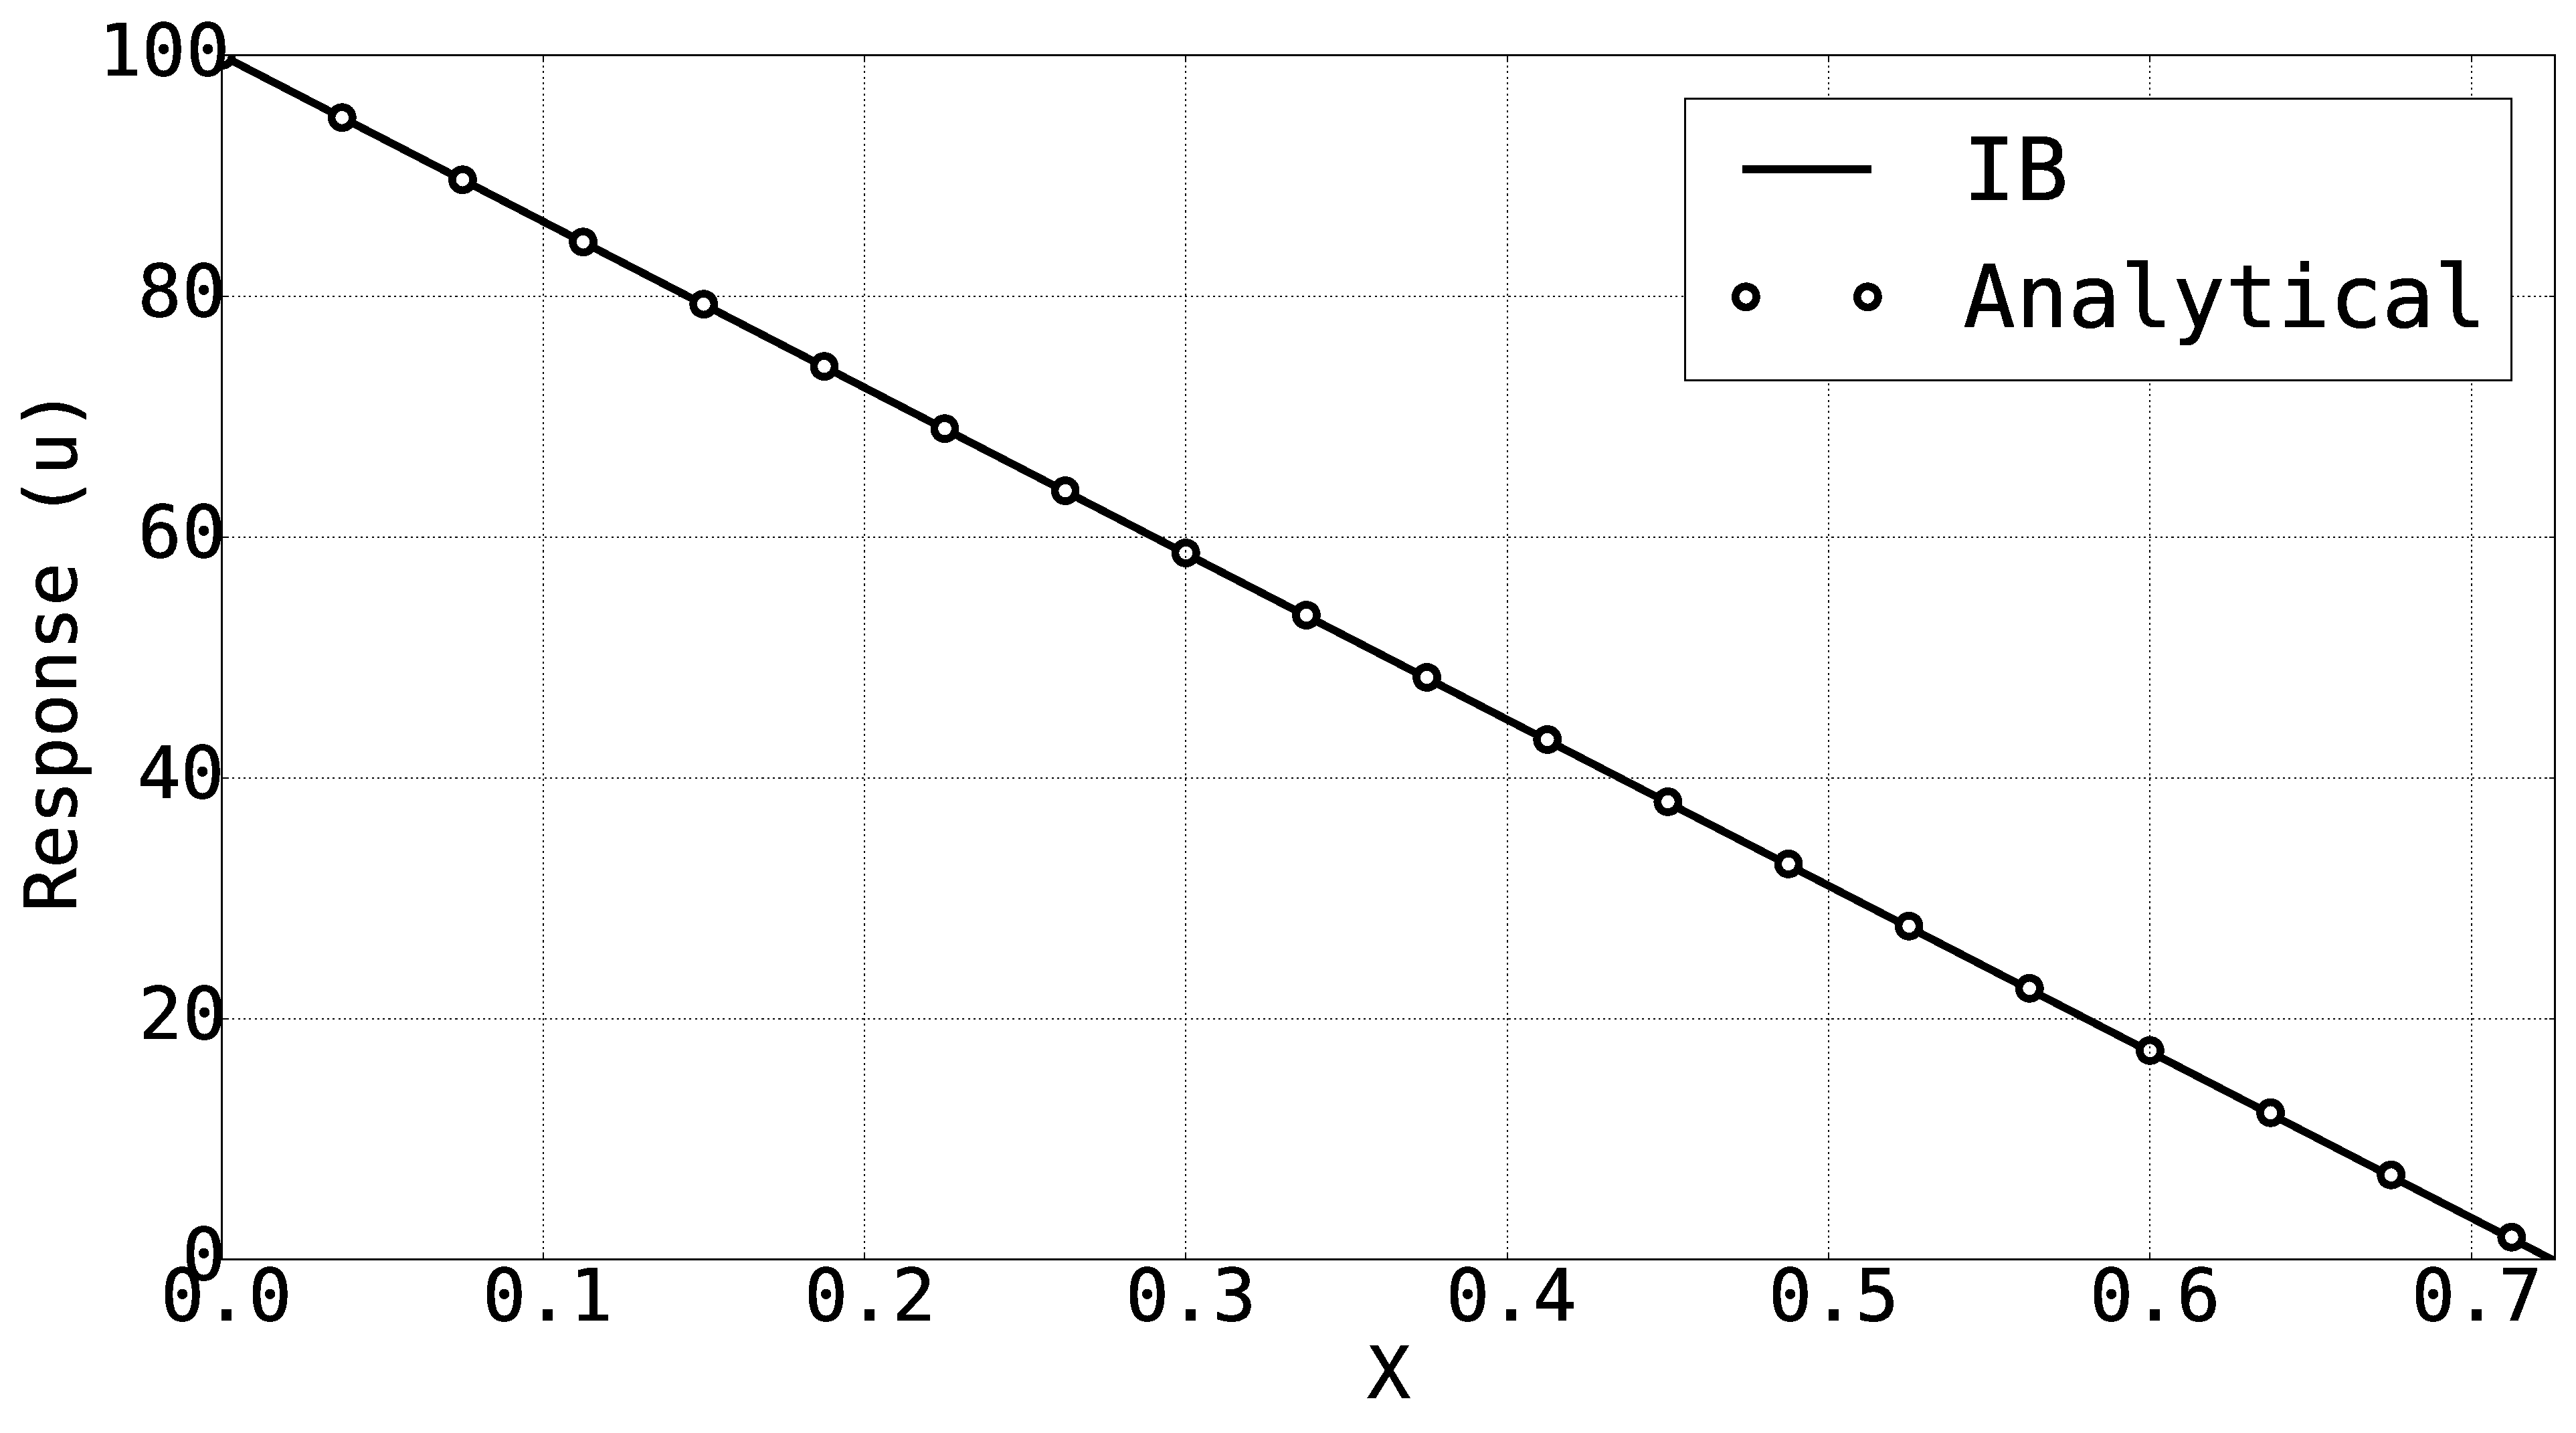
\includegraphics[width=7.0cm]{Chapter_3/figure/virtualBoundary_wallVelocity_100.eps}
	}
	\\
	\subfigure[$u_{wall} = 10^3 m/s$]
	{
	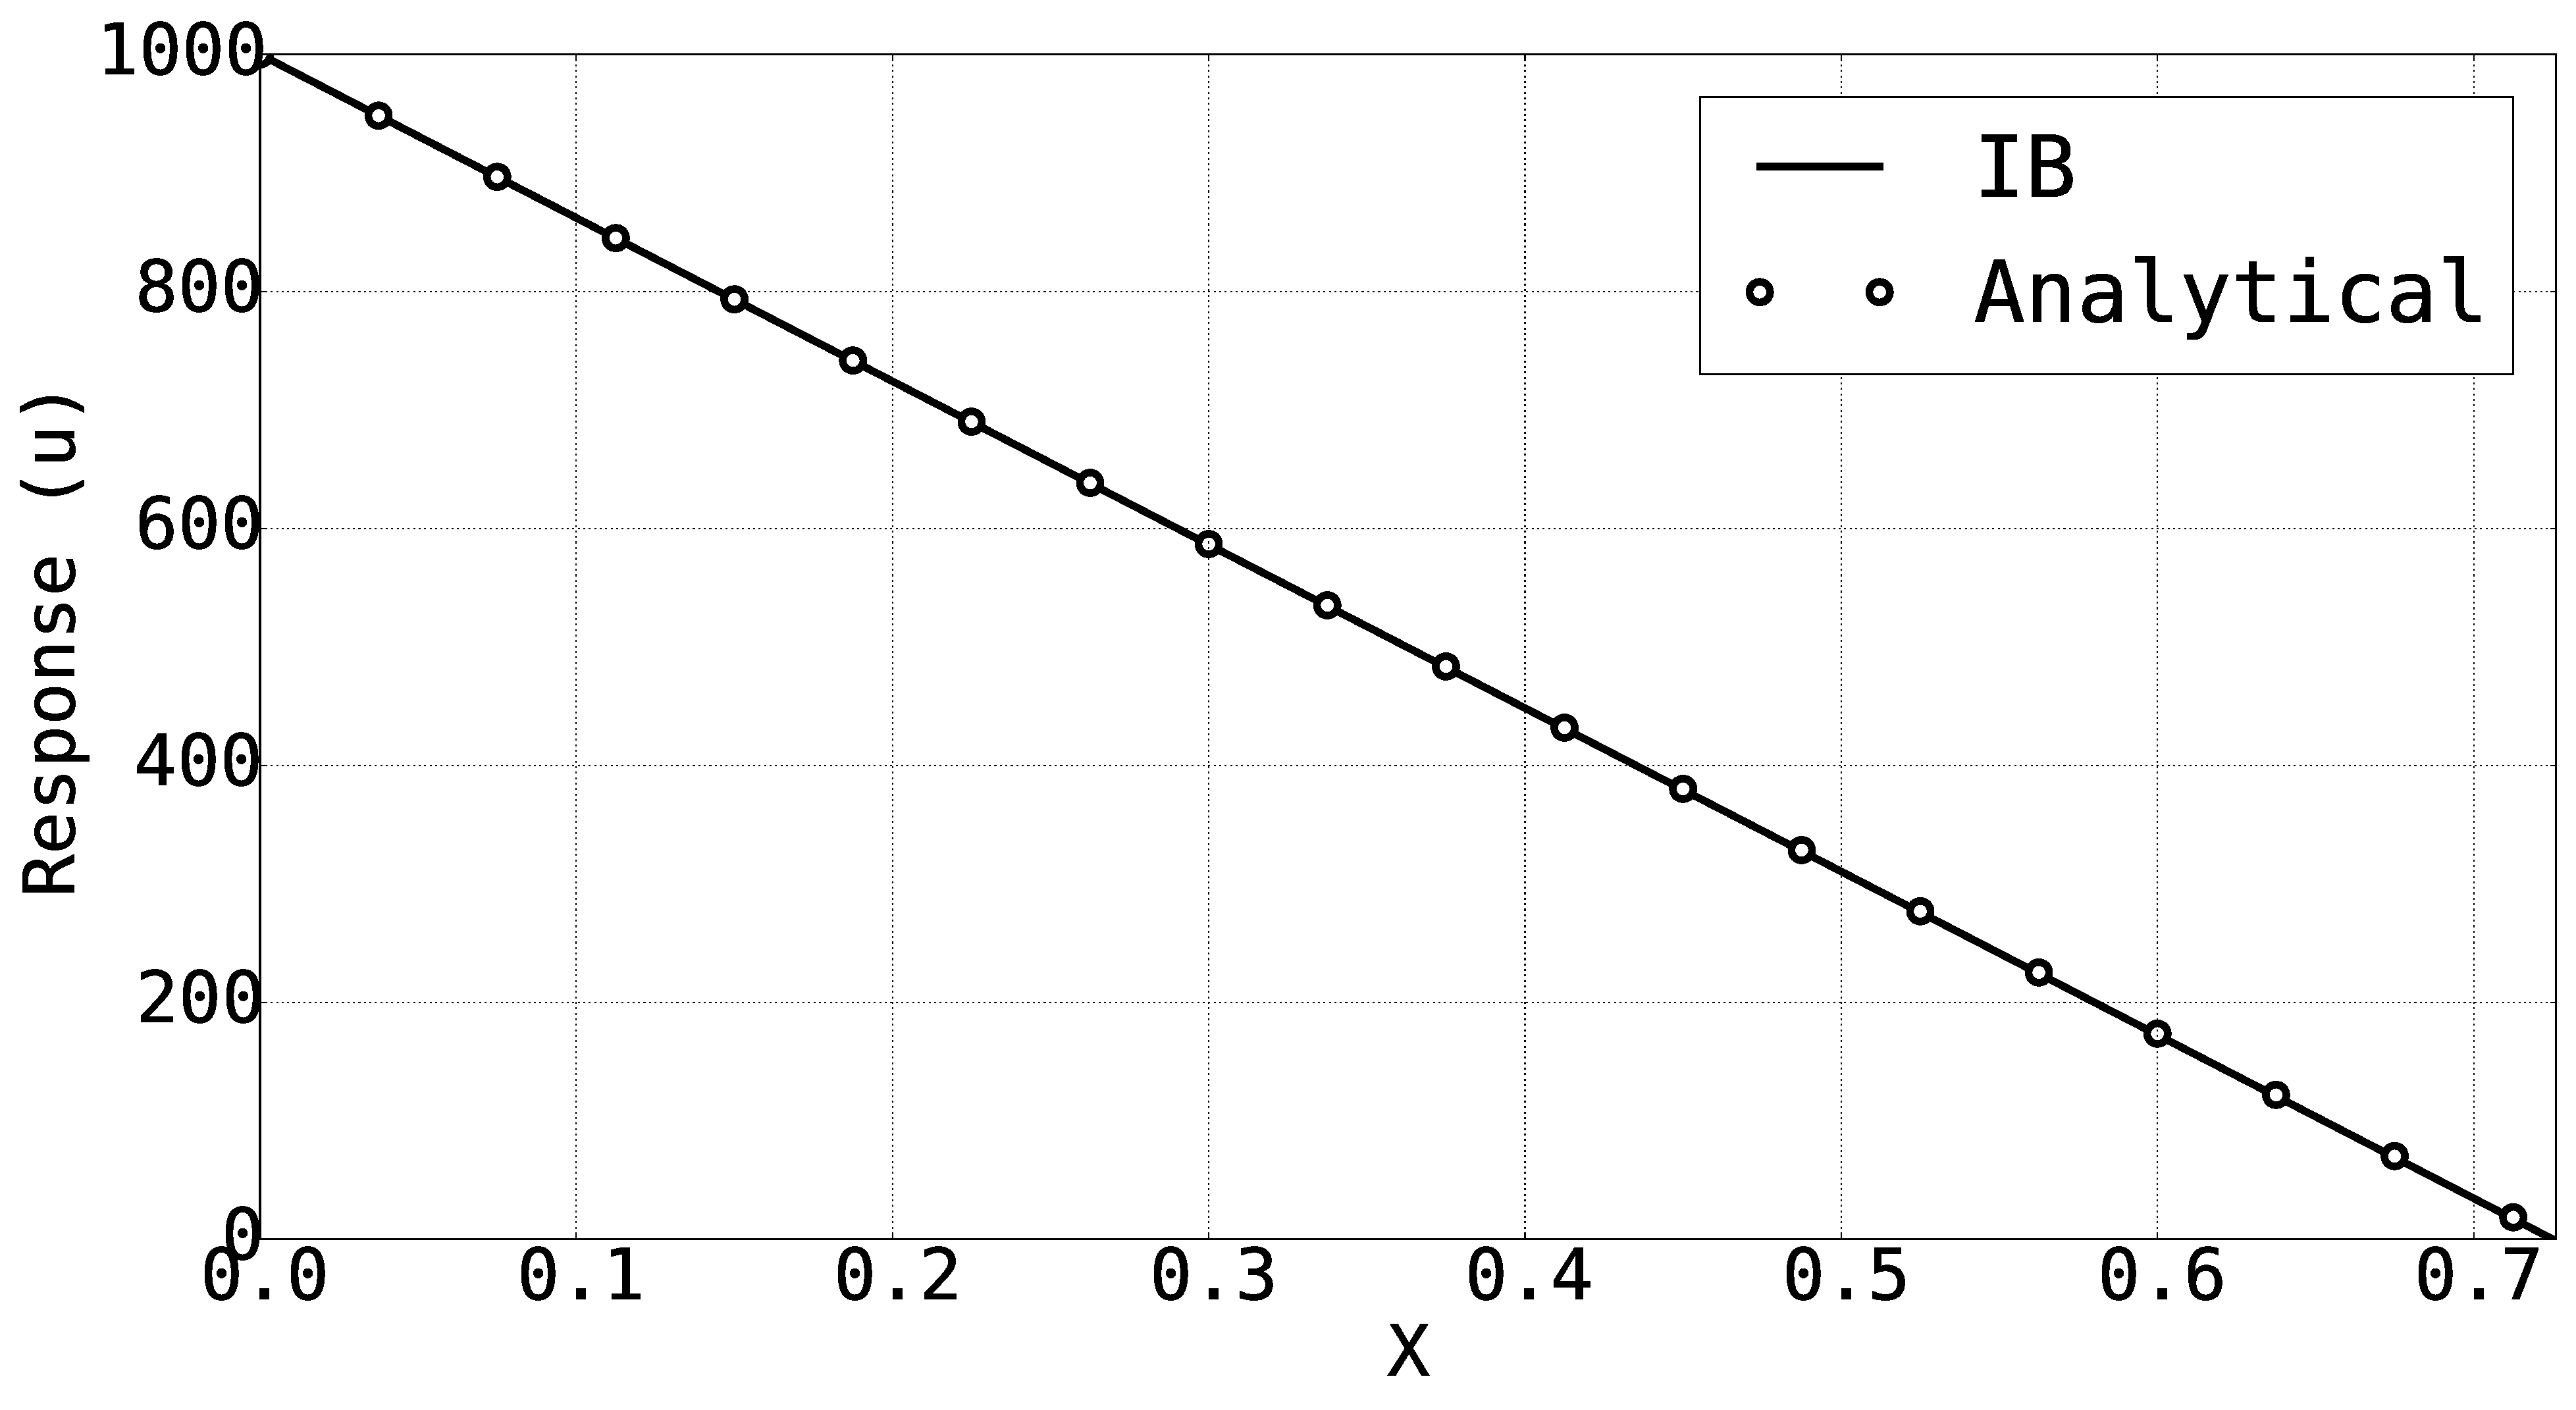
\includegraphics[width=7.0cm]{Chapter_3/figure/virtualBoundary_wallVelocity_1000.eps}
	}
	\quad
	\subfigure[$u_{wall} = 10^4 m/s$]
	{
	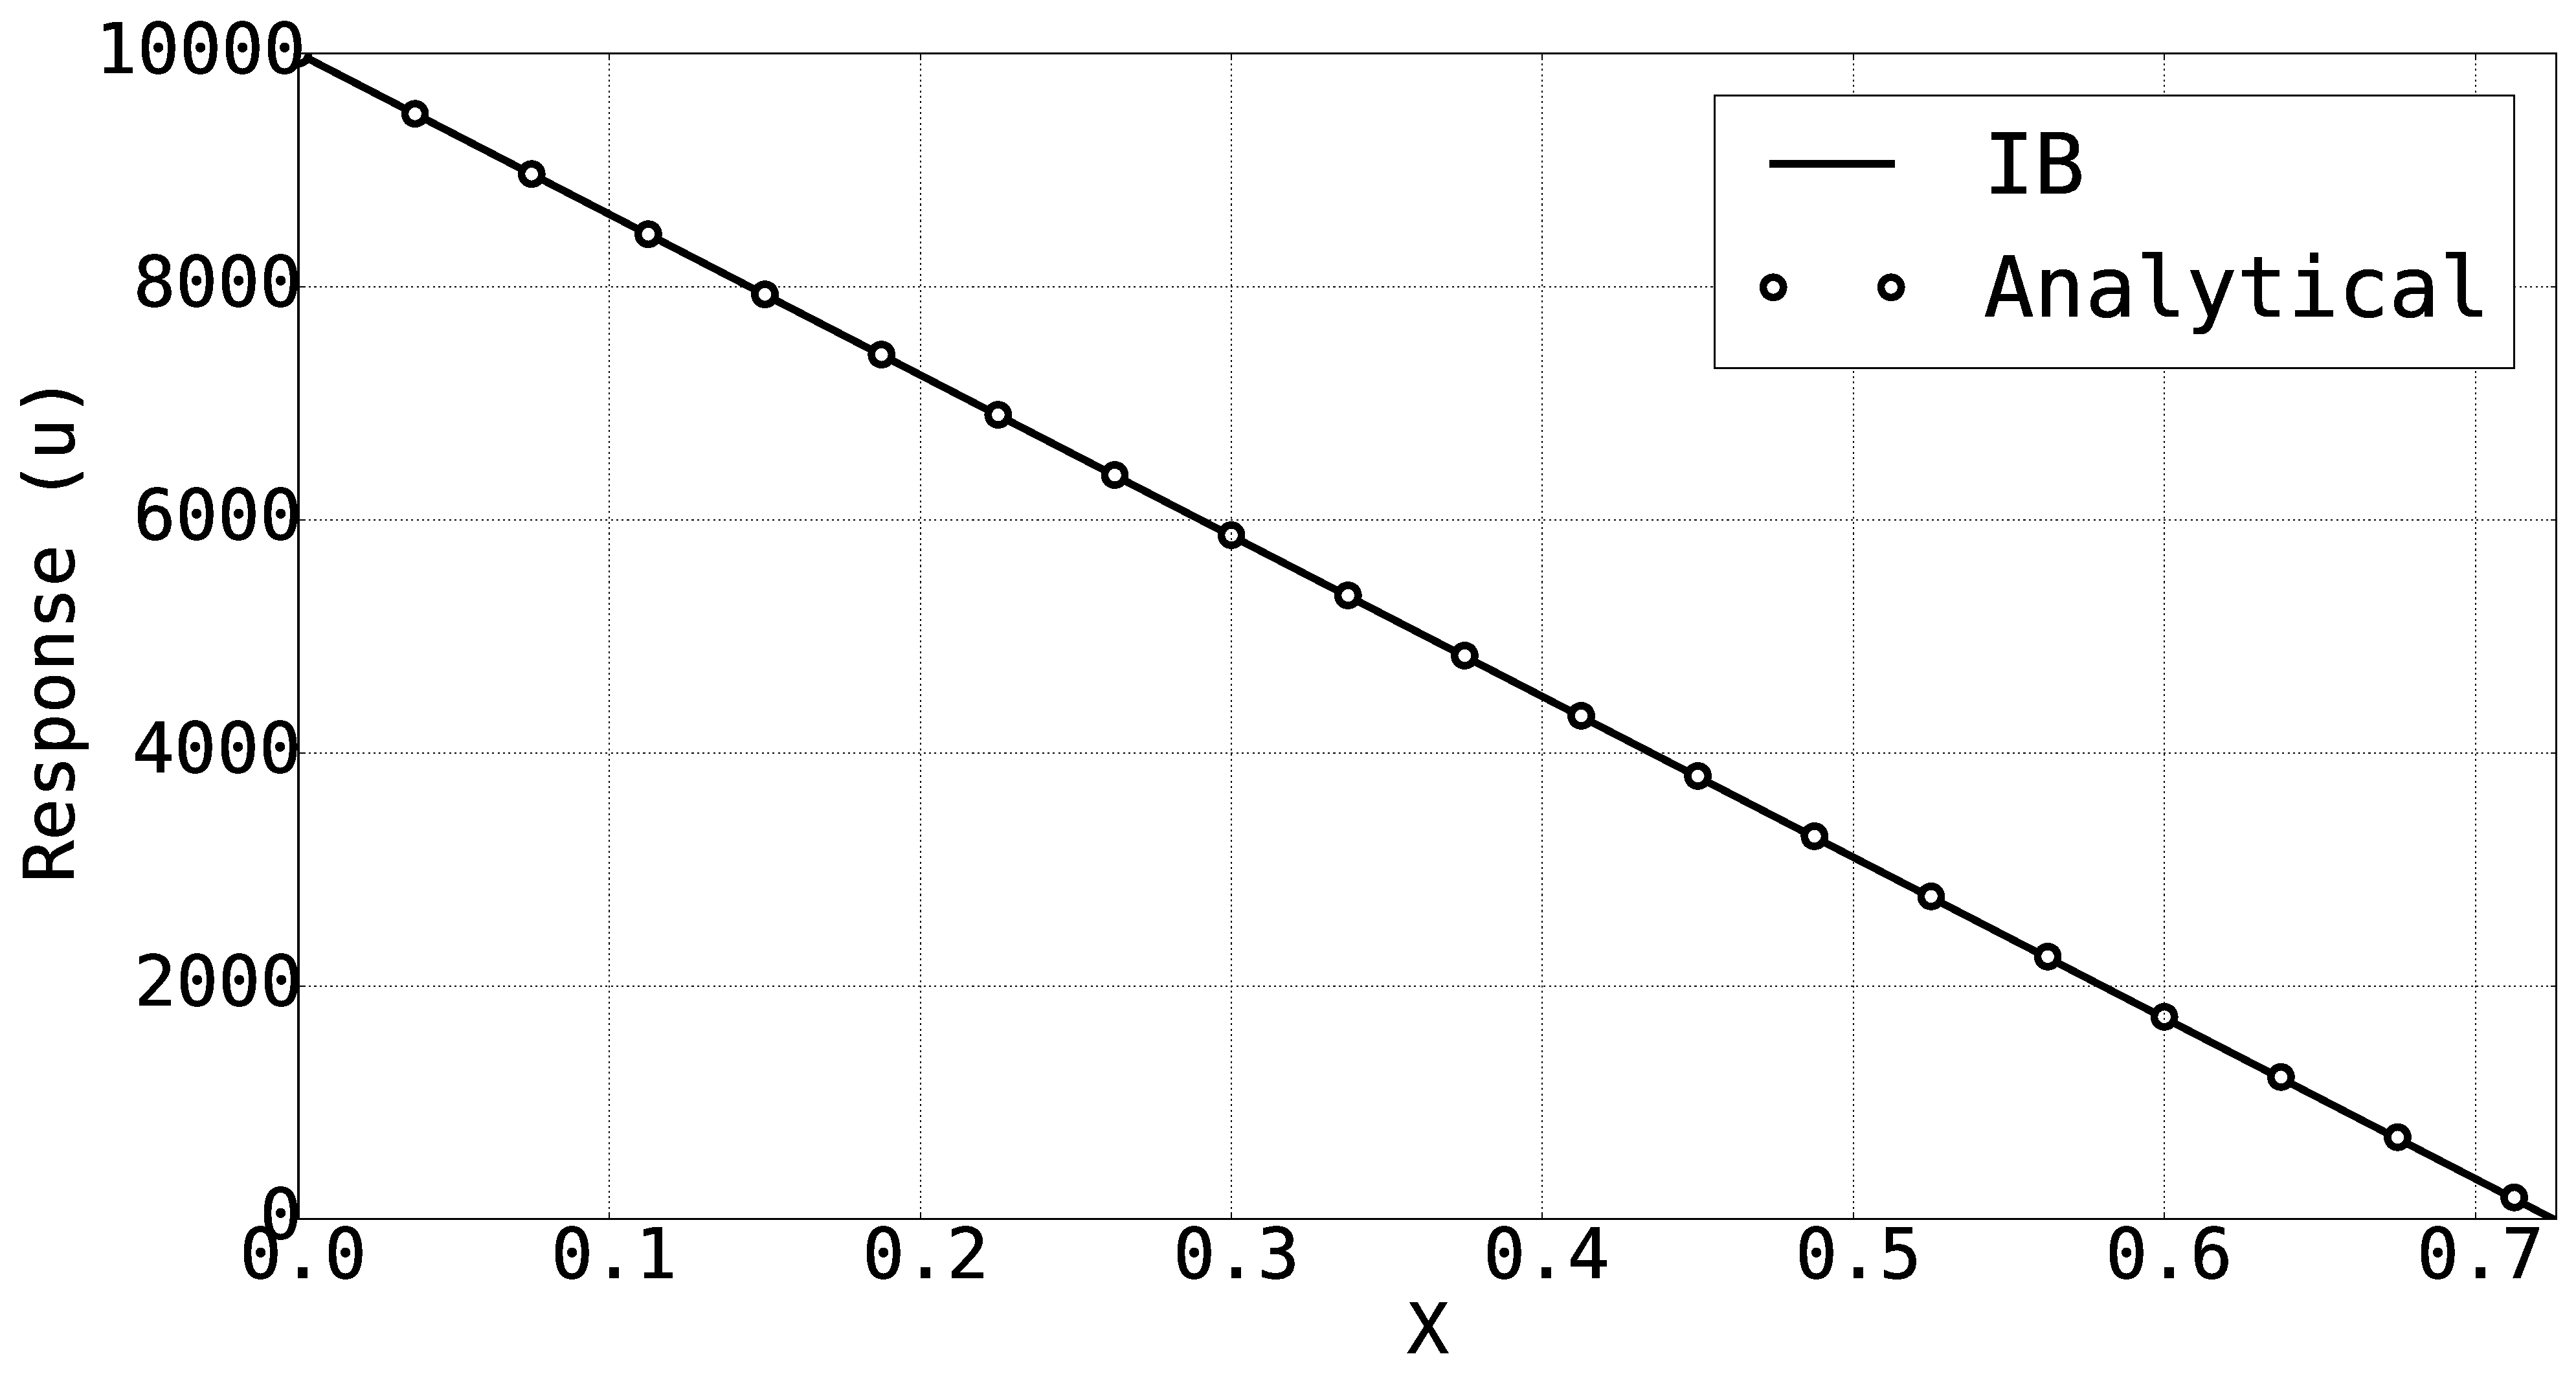
\includegraphics[width=7.0cm]{Chapter_3/figure/virtualBoundary_wallVelocity_10000.eps}
	}
	\caption{Comparison between IB and analytical results for different wall velocities.}
	\label{fig:C3_virtualBoundaryResultWallVelocity}
\end{figure}

\begin{table}[H]
\centering
\begin{tabular}{c | c}
	 Wall velocity & RMSE \\ \hline \hline
	 10 & 0.000616\\ \hline
	 $10^2$ & 0.000616 \\ \hline
	 $10^3$ & 0.000616 \\ \hline
	 $10^4$ & 0.000616 \\
\end{tabular}
\caption{RMSE value for different wall velocities.}
\label{table:C3_virtualBoundaryResultWallVelocityRMSE}
\end{table}

Finally we looked at the effect of constants $\alpha$ and $\beta$ on the accuracy of the solution. We discretized the domain using $81$ nodes with wall velocity equal to $100$ with time step equal to $10^{-5}$. The location of the fixed wall is chosen as $x_{wall} = 0.726$. The flow between the plates is modelled using different coefficients for $\alpha$ and $\beta$ as shown in Table \ref{table:C3_alphaBetaValues}.

\begin{table}[H]
\centering
\begin{tabular}{c | c | c}
	 Case number & $\alpha$ & $\beta$ \\ \hline \hline
	 1 & -10 & -10 \\ \hline
	 2 & -100 & -10 \\ \hline
	 3 & -100 & -1 \\ \hline
	 4 & -100 & -100 \\
\end{tabular}
\caption{Different values used for investigating the effect of $\alpha$ and $\beta$.}
\label{table:C3_alphaBetaValues}
\end{table}

As can be seen in Figure \ref{fig:C3_virtualBoundaryResultConstant} and Table \ref{fig:C3_virtualBoundaryResultConstantRSME}, $\alpha$ value has a considerable effect of the accuracy of the results. Increasing the $\alpha$ value with an order of magnitude results in a considerable improvement in the accuracy of the solution. However, $\beta$ value does not contribute to the accuracy but improves the stability of the solution. The solutions with larger $\beta$ values converged in less number of iterations.

\begin{figure}[H]
	\centering
	\subfigure[$\alpha = -10, \beta = -10$]
	{
	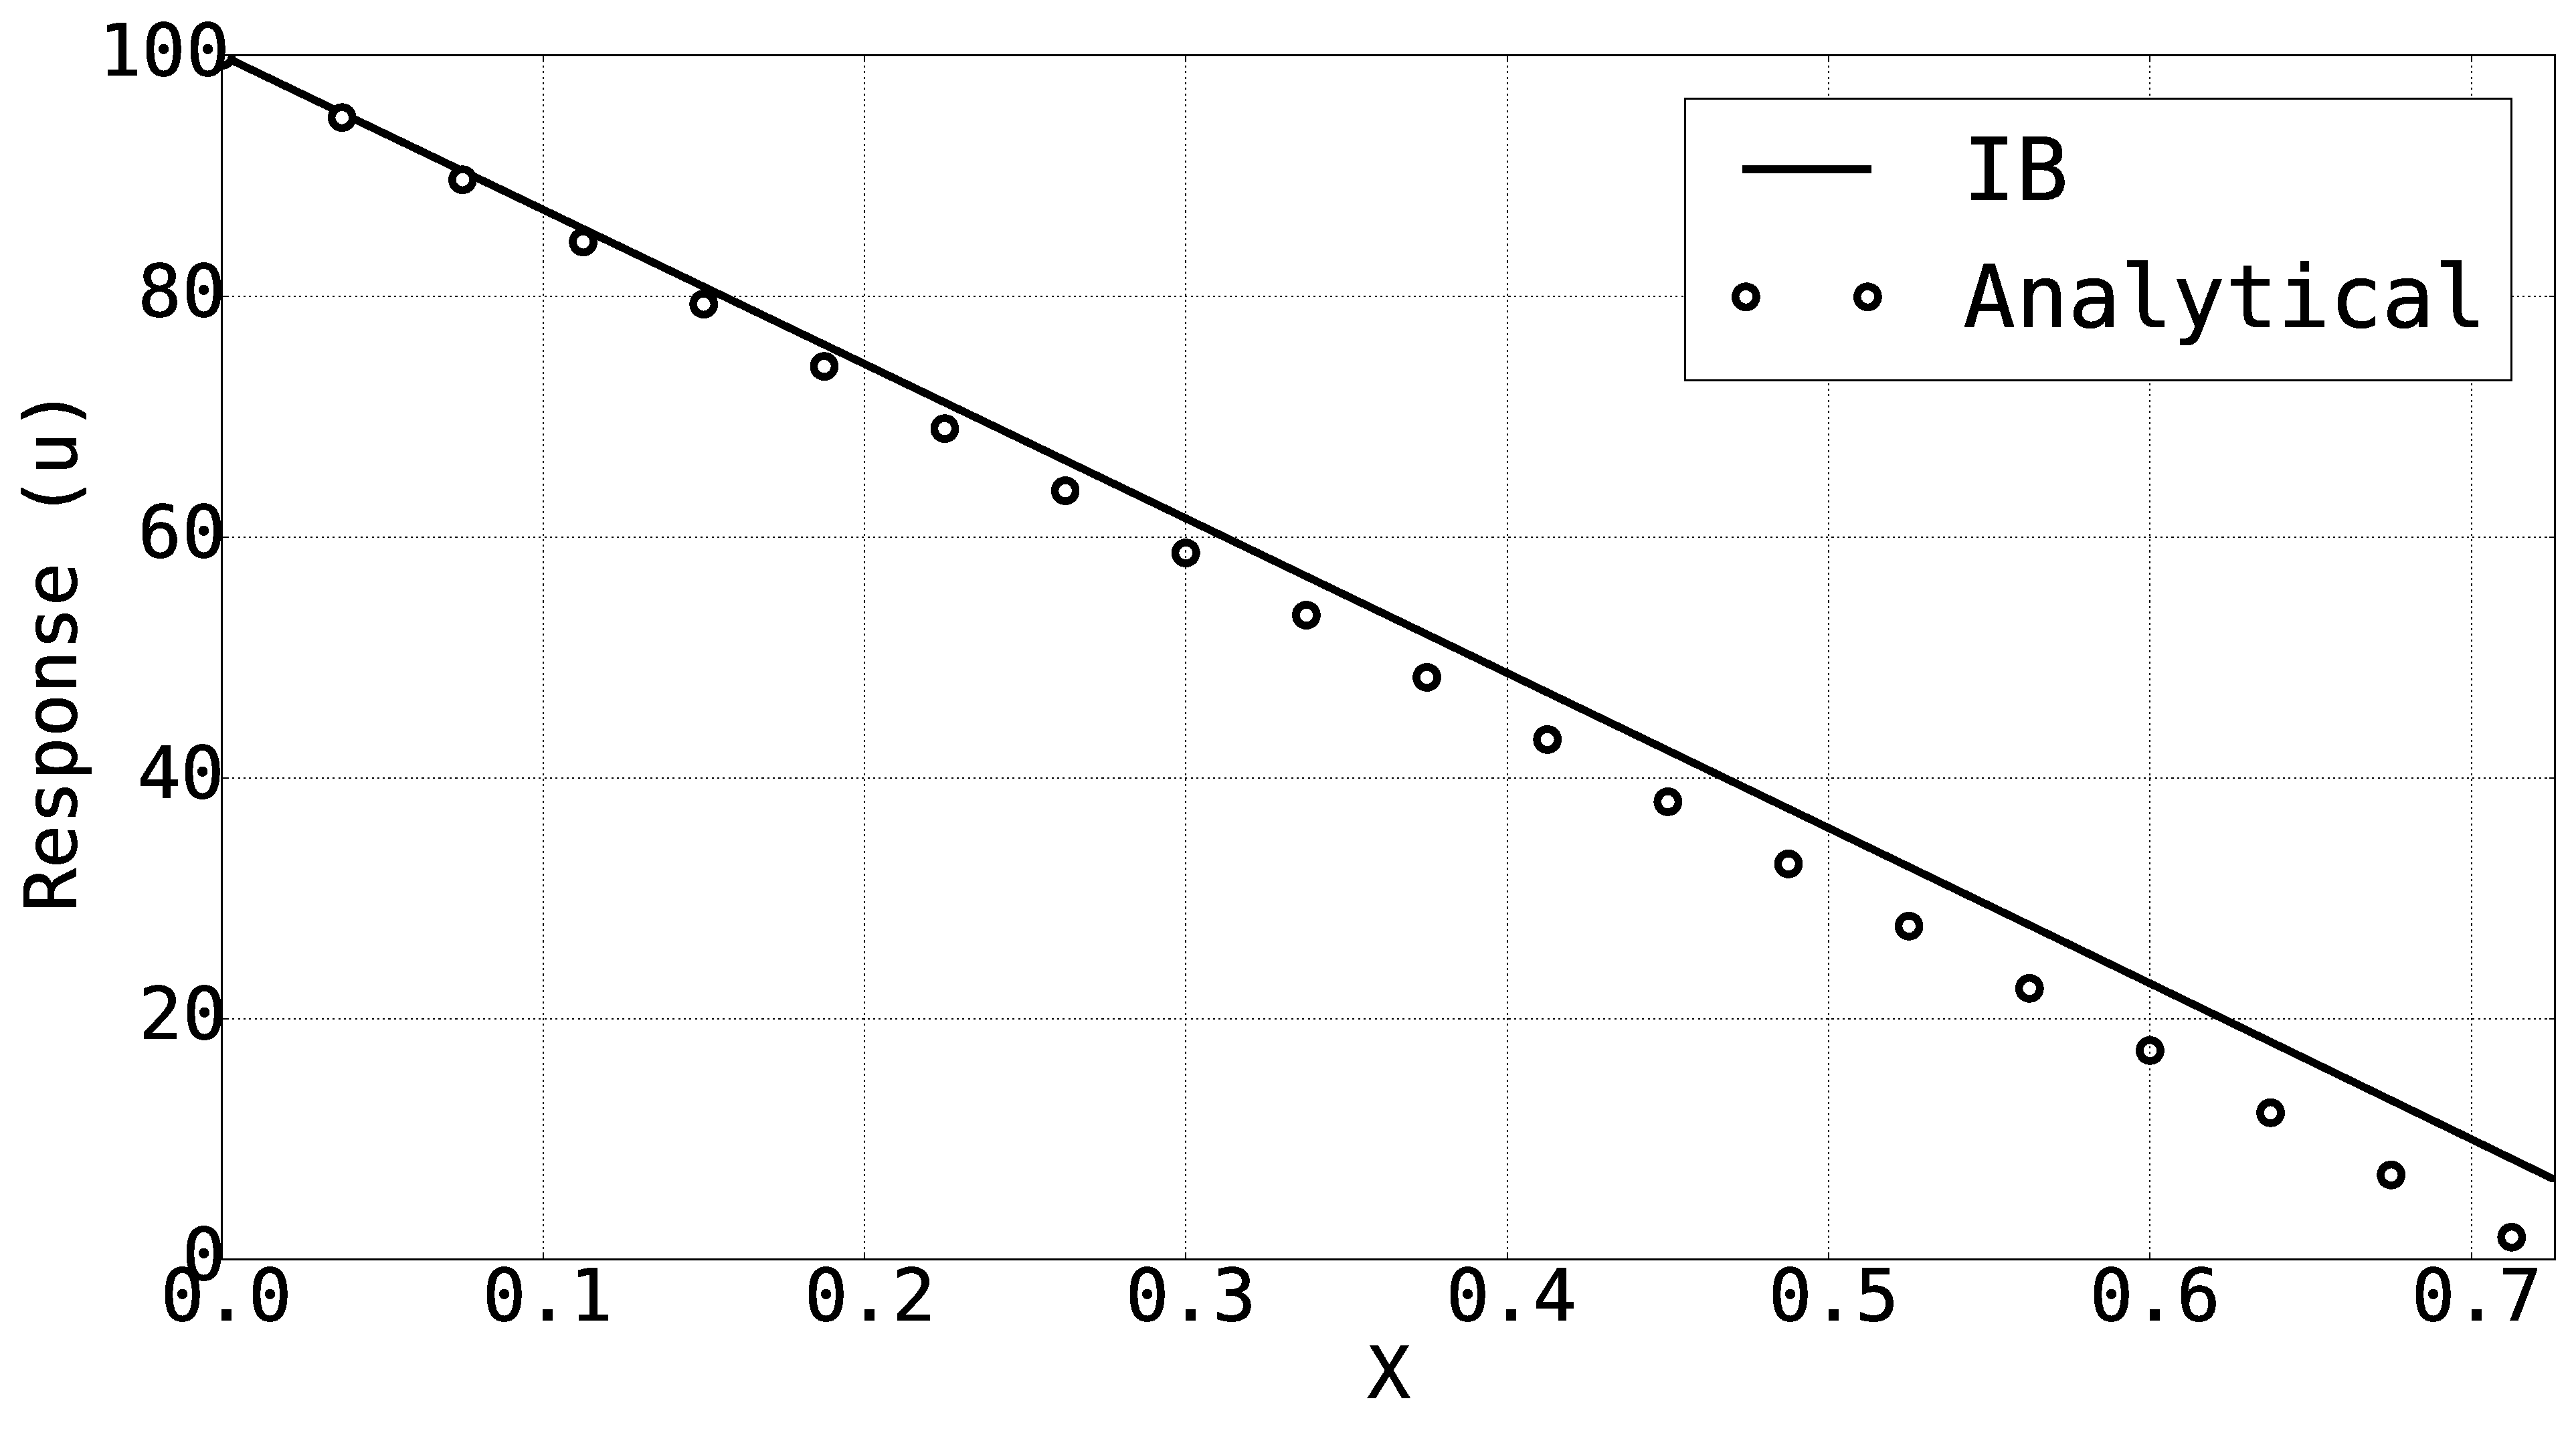
\includegraphics[width=7.0cm]{Chapter_3/figure/virtualBoundary_constant_alpha_10_beta_10.eps}
	}
	\quad
	\subfigure[$\alpha = -100, \beta = -10$]
	{
	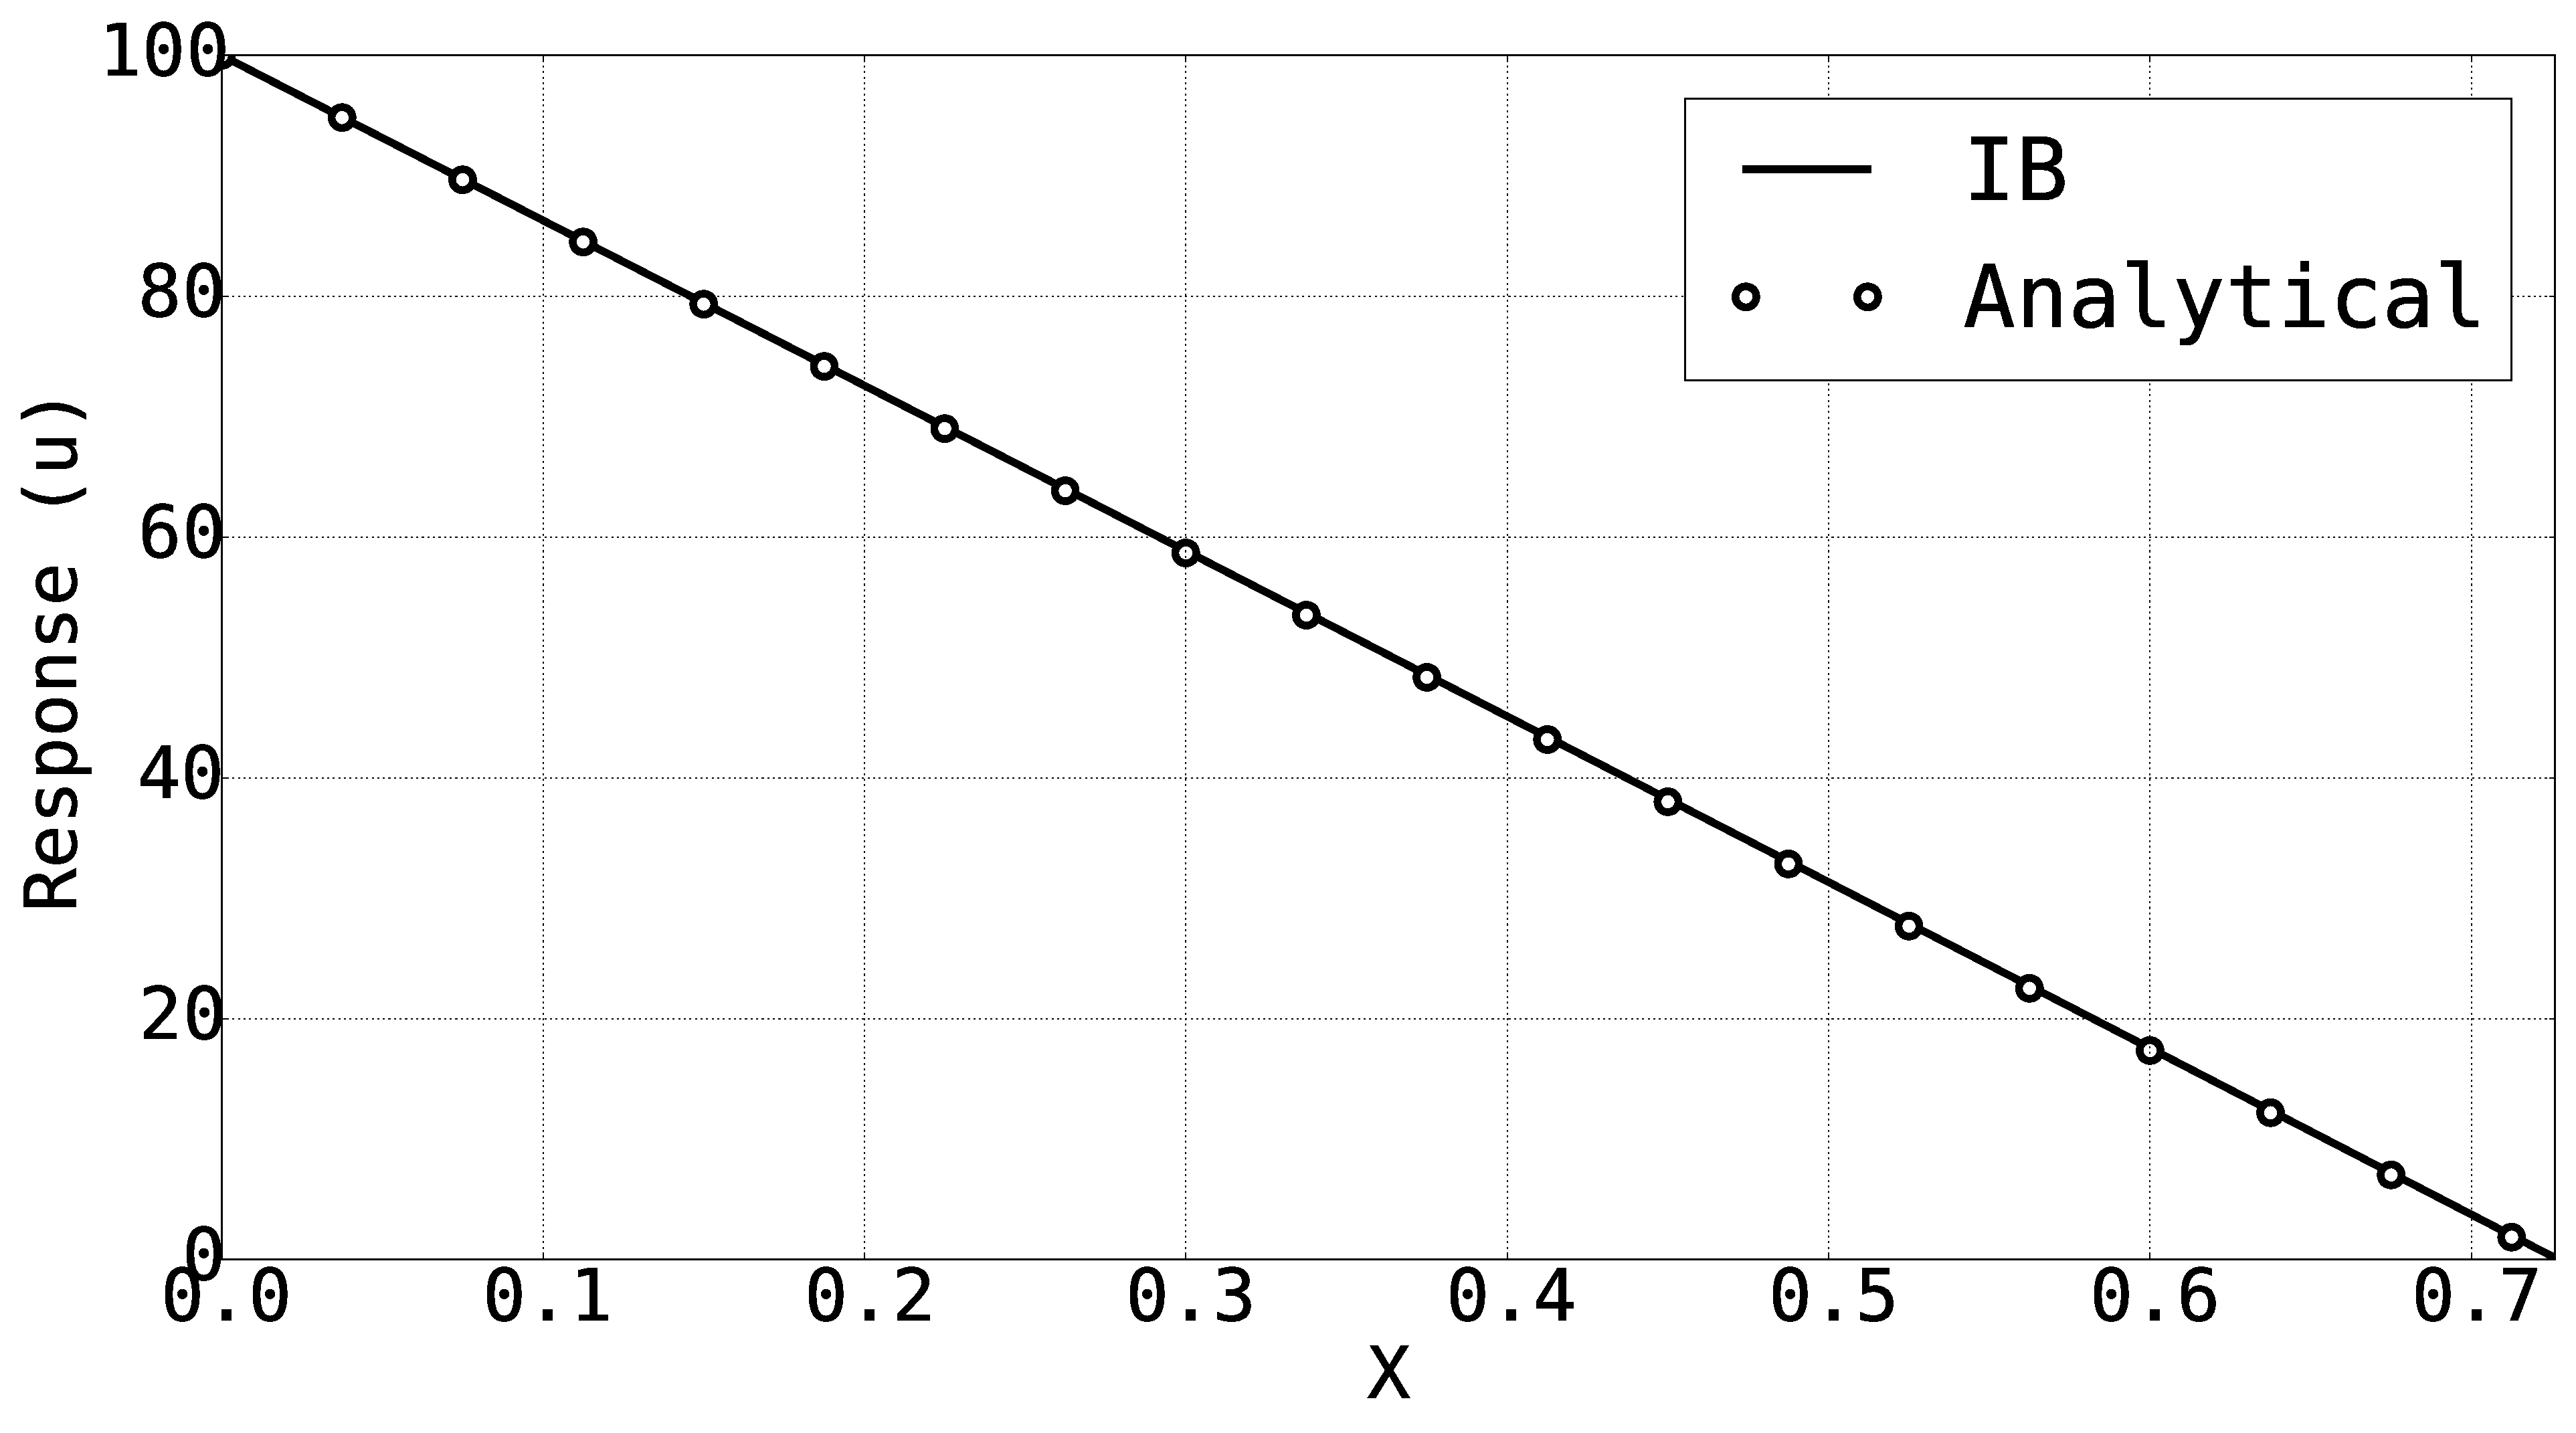
\includegraphics[width=7.0cm]{Chapter_3/figure/virtualBoundary_constant_alpha_100_beta_10.eps}
	}
	\\
	\subfigure[$\alpha = -100, \beta = -1$]
	{
	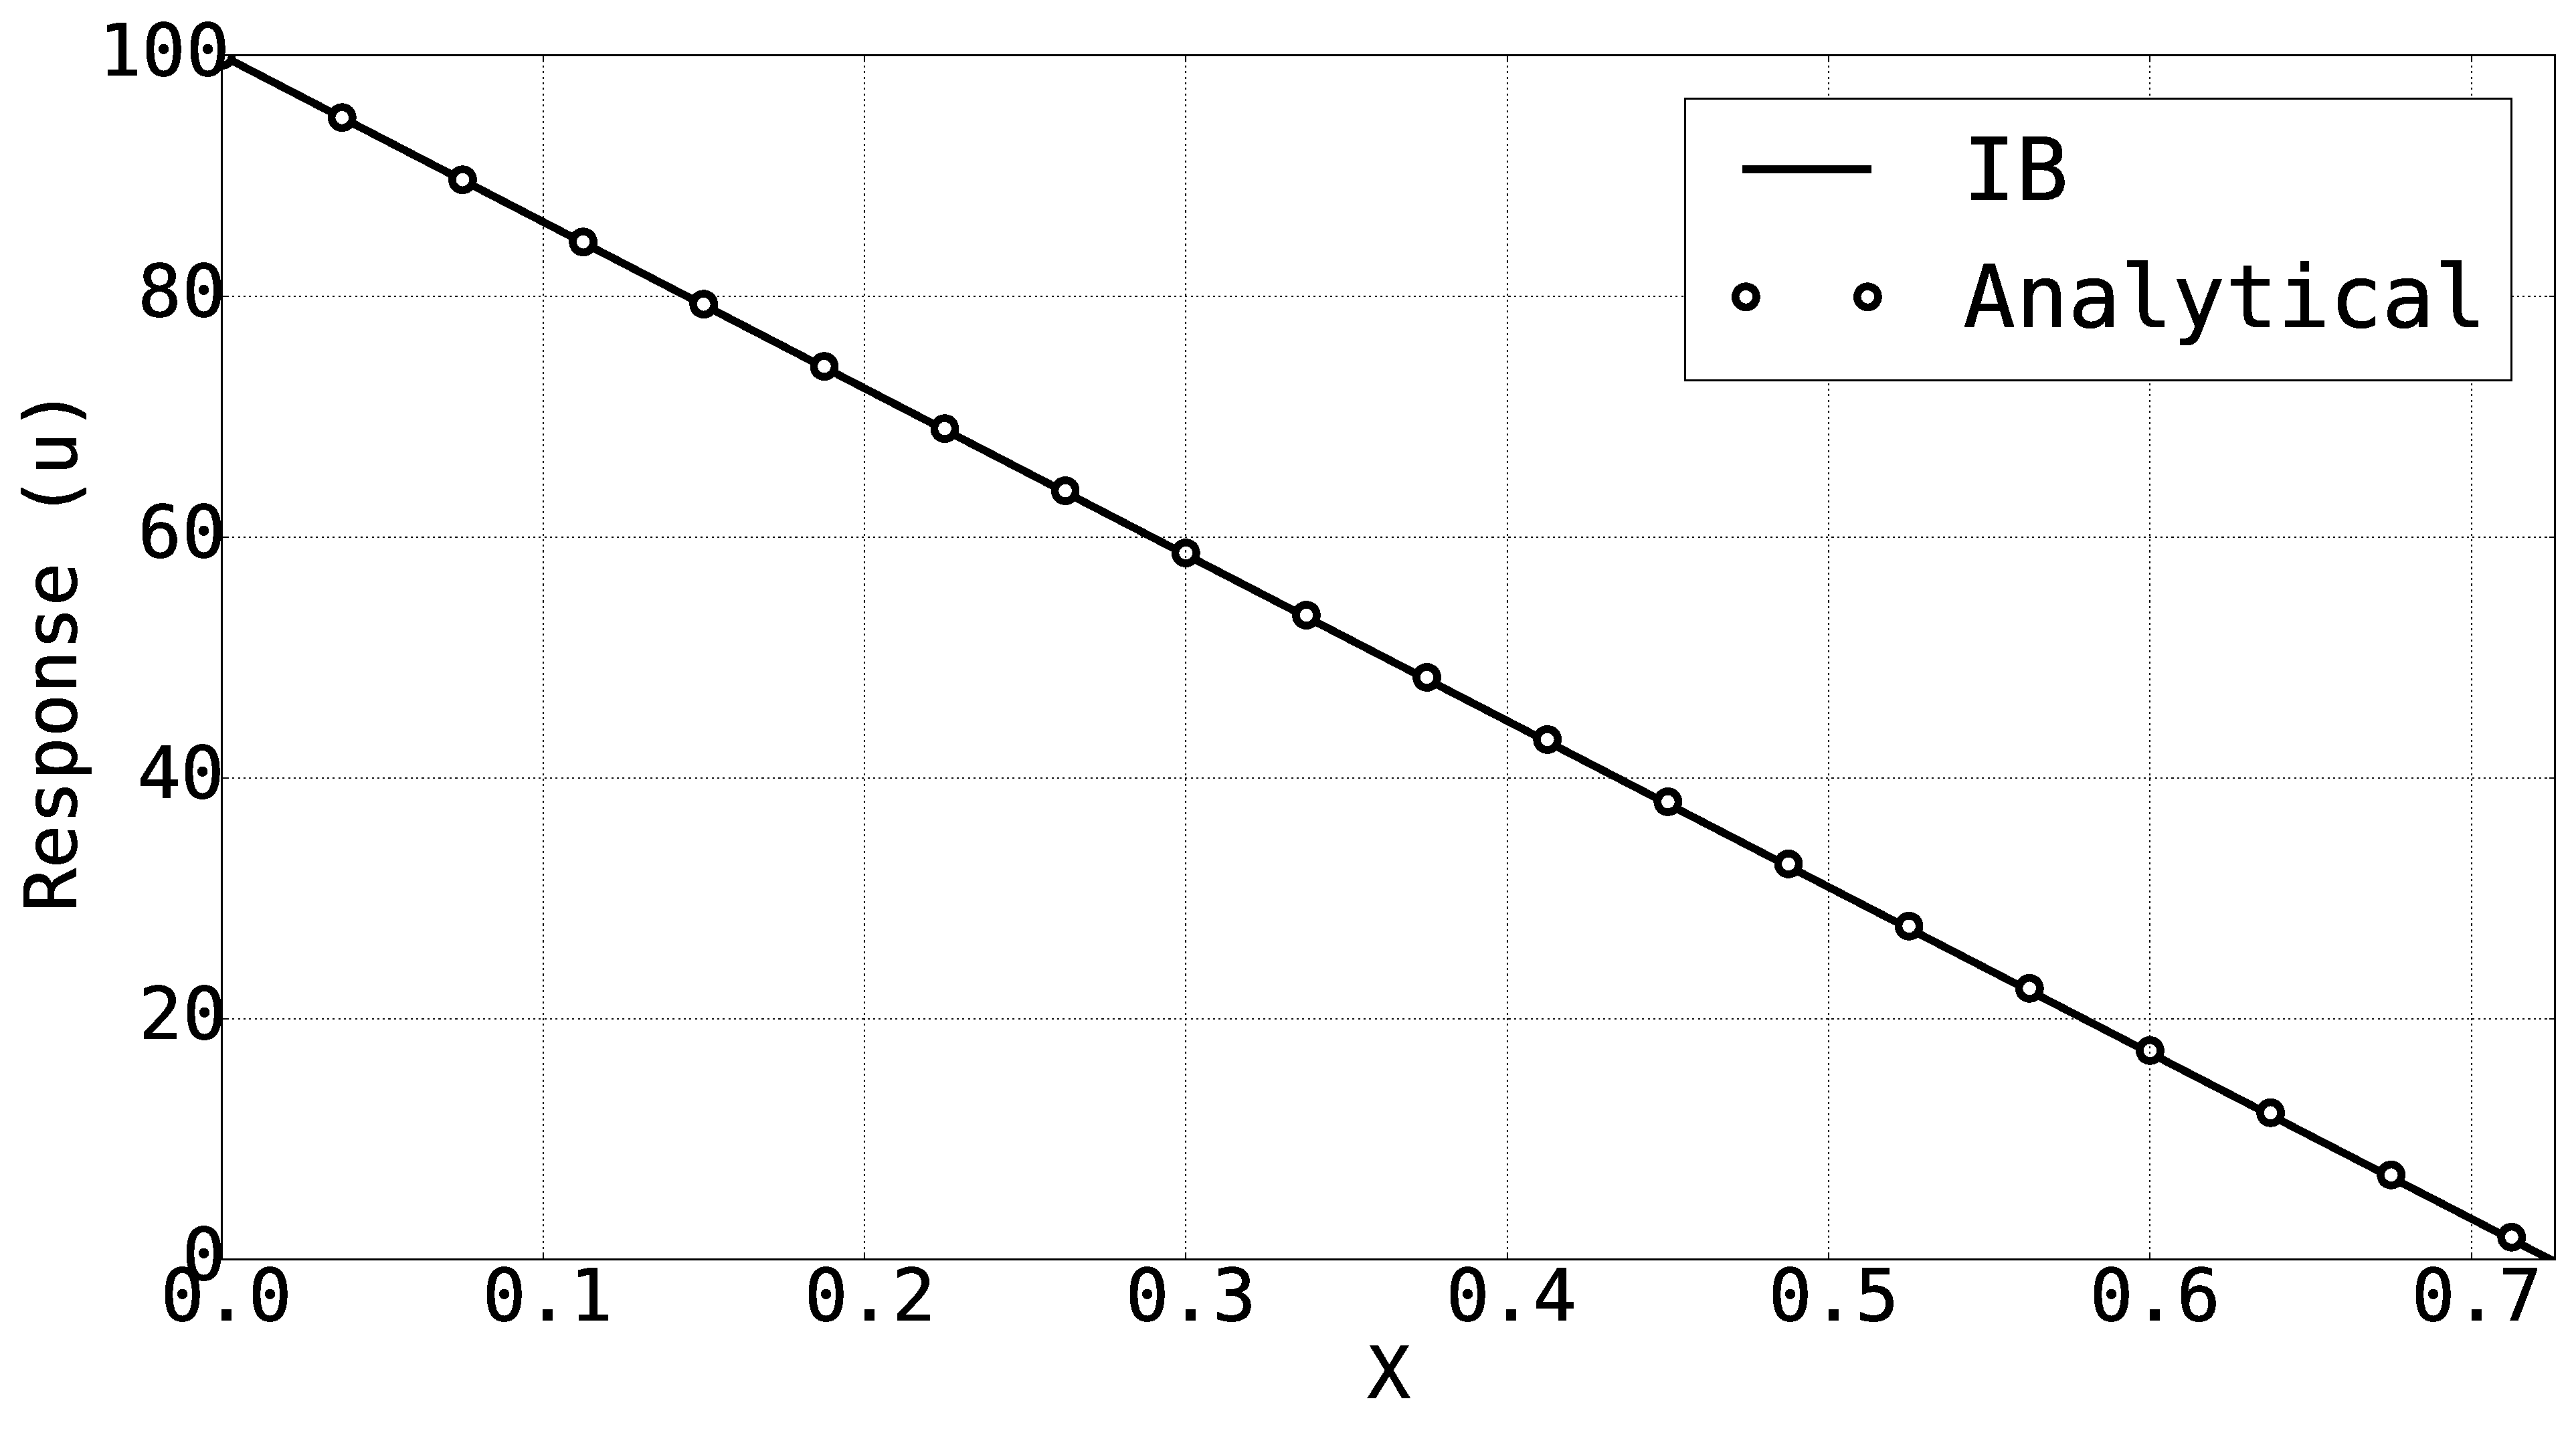
\includegraphics[width=7.0cm]{Chapter_3/figure/virtualBoundary_constant_alpha_100_beta_1.eps}
	}
	\quad
	\subfigure[$\alpha = -100, \beta = -100$]
	{
	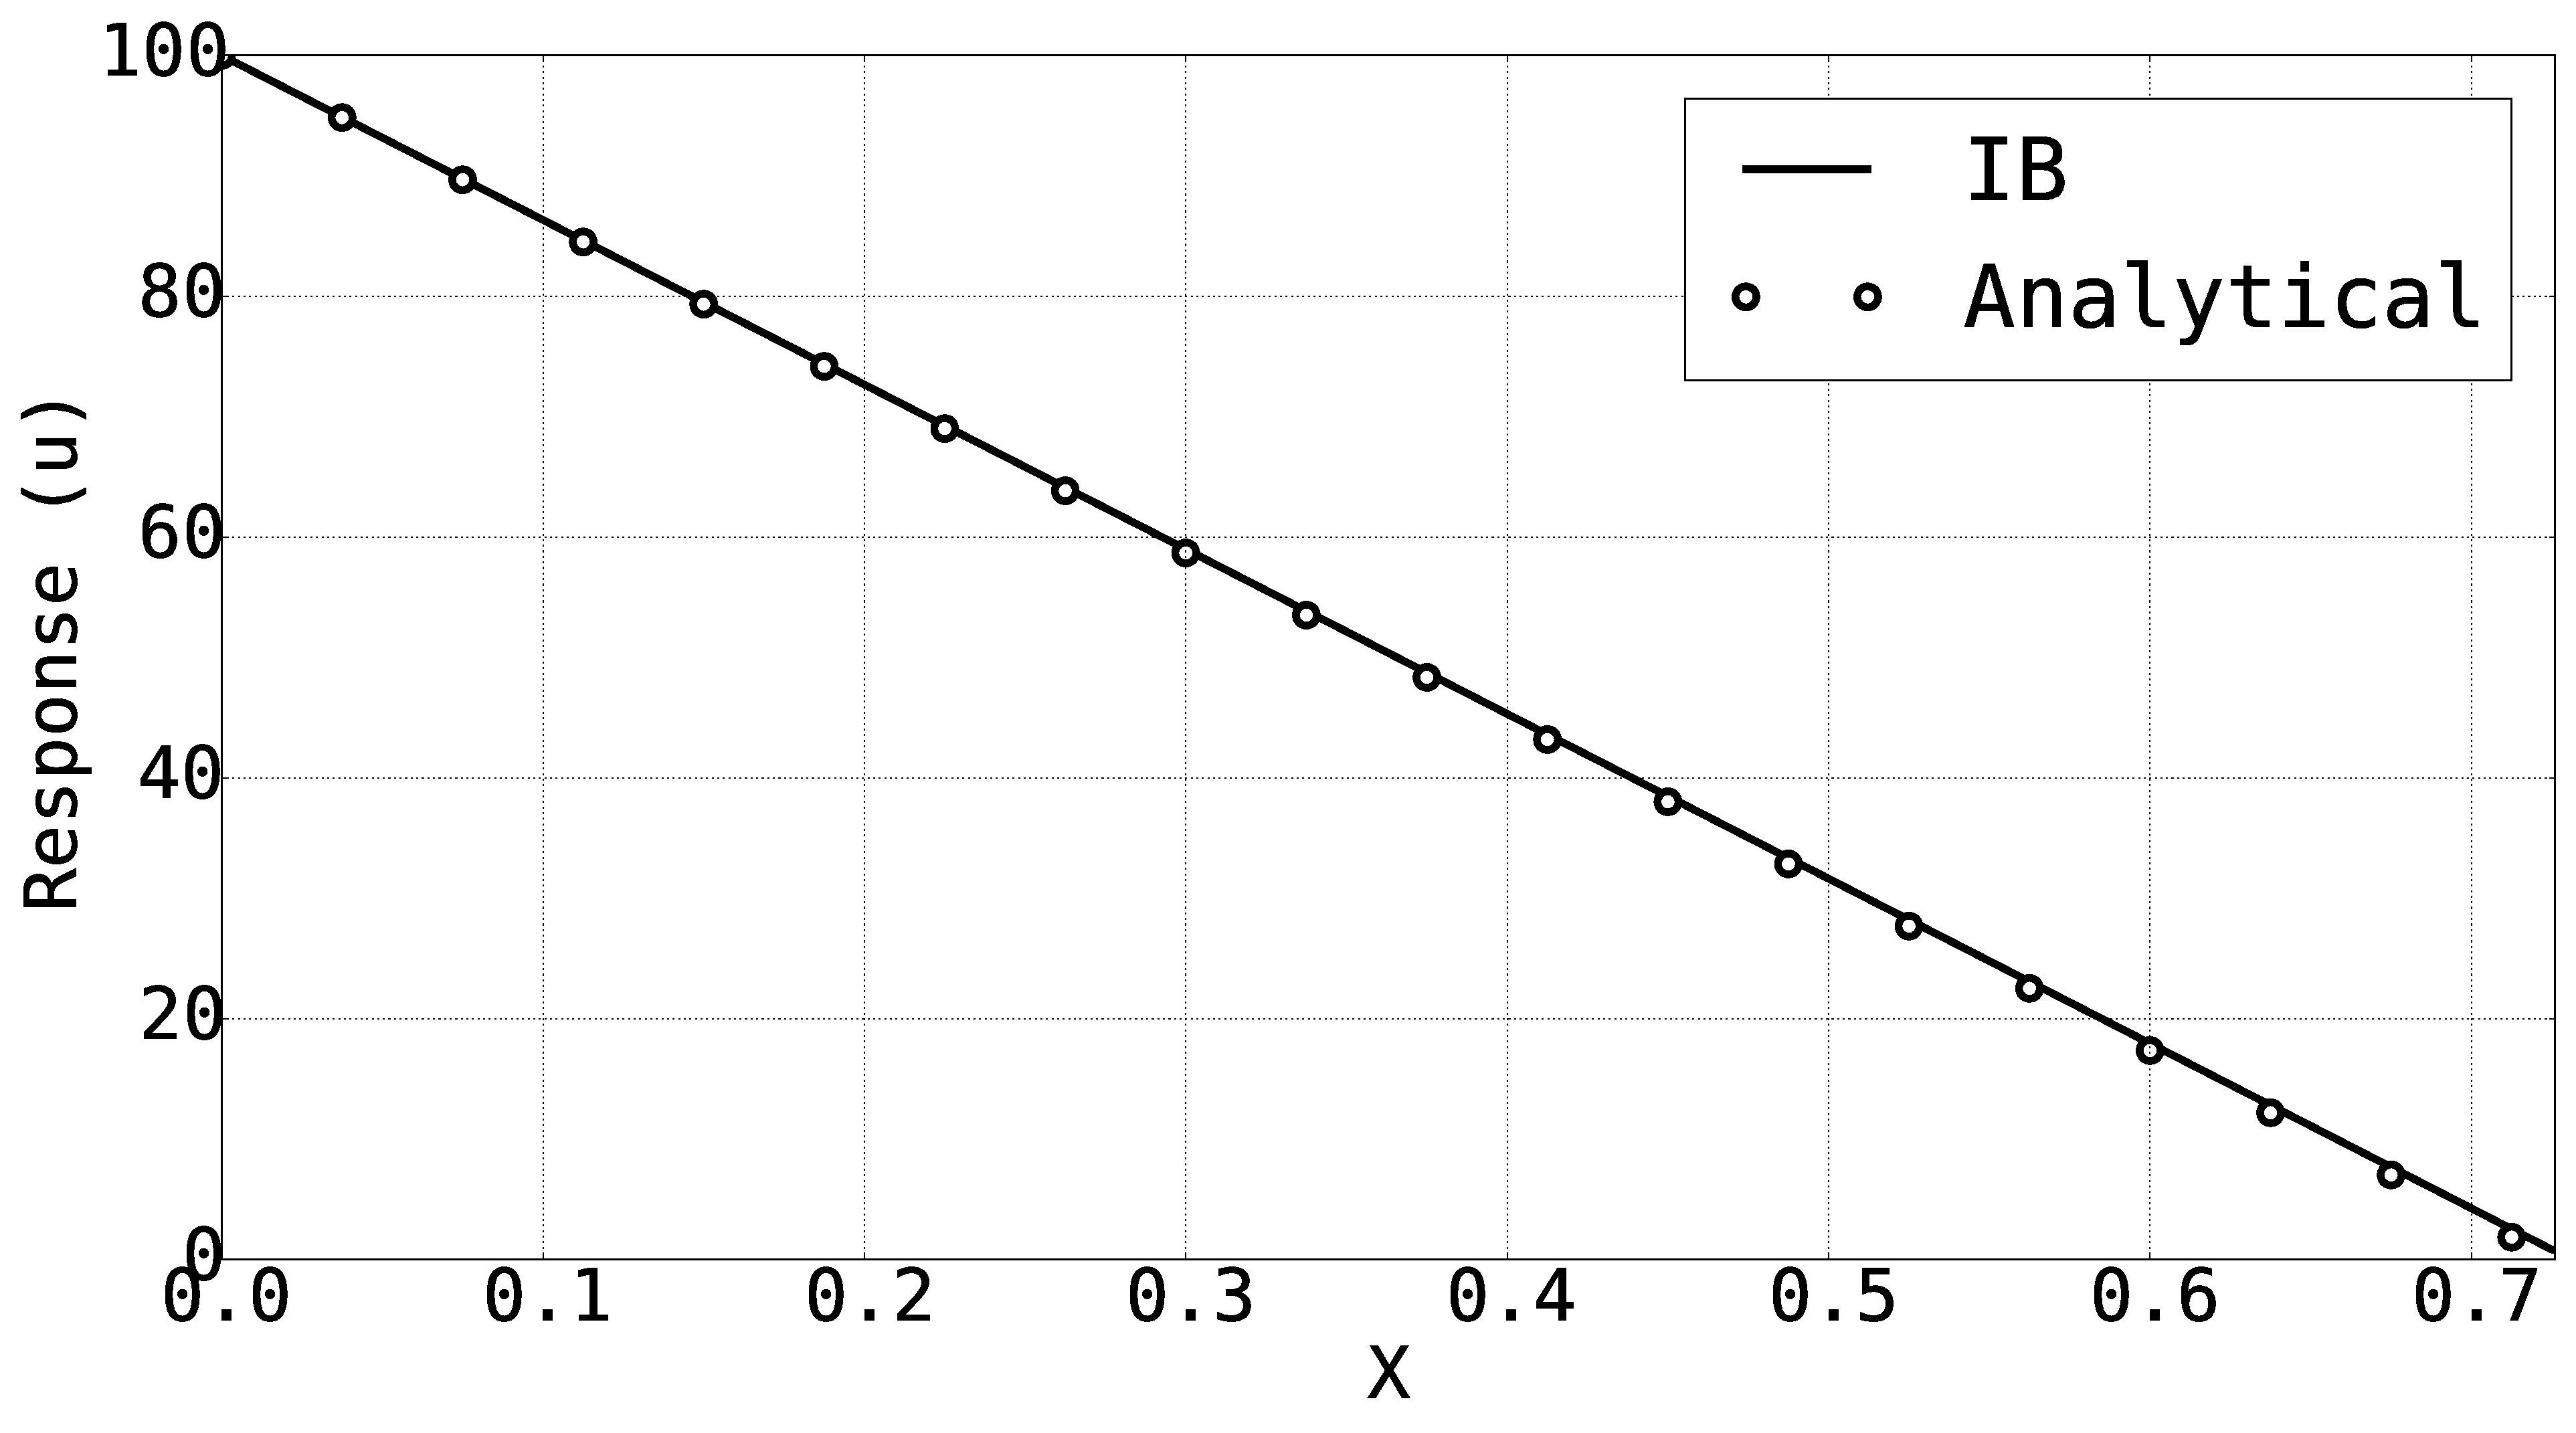
\includegraphics[width=7.0cm]{Chapter_3/figure/virtualBoundary_constant_alpha_100_beta_100.eps}
	}
	\caption{Comparison between IB and analytical results for different wall velocities.}
	\label{fig:C3_virtualBoundaryResultConstant}
\end{figure}

\begin{table}[H]
\centering
\begin{tabular}{c | c | c}
	 $\alpha$ & $\beta$ & RMSE \\ \hline \hline
	 -10 & -10 & 0.0327 \\ \hline
	 -100 & -10 & 0.00138 \\ \hline
	 -100 & -1 & 0.00129 \\ \hline
	 -100 & -100 & 0.00346 \\
\end{tabular}
\caption{Different values used for investigating the effect of $\alpha$ and $\beta$.}
\label{table:C3_virtualBoundaryResultConstantRSME}
\end{table}
% -.-.-.-.-.-.-.-.-.-.-.-.-.-.-.-.-.-.-.-.-.-.-.-.-.-.-.-.-.-.-.-.-.-
\subsection{Penalization method}
The third class of continuum immersed boundary techniques are known as penalization method that was first introduced by Arquis and Caltagirone \cite{ arquis1984conditions}. In this method, the solid boundaries are modeled as porous media. Porosity or void fraction is a measure of the void spaces in a material, and is a fraction of the volume of voids over the total volume, between 0 and 1. For the solid domain the porosity value is near zero whereas for the fluid domain its value is close to one. Flow through a porous domain is described using the Darcy's law. This is a simple proportional relationship between the instantaneous discharge rate through a porous medium, the viscosity of the fluid and the pressure drop over a given distance.

\begin{figure}[H]
	\centering
	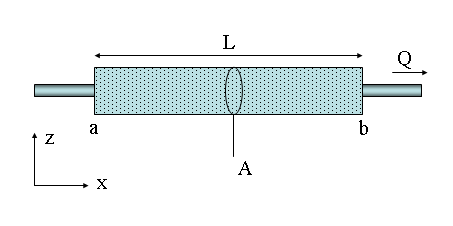
\includegraphics[width=14.cm]{Chapter_3/figure/Darcys_Law.png}
	\caption{Flow through a porous pipe.}
\end{figure}

For a flow through a porous domain in a pipe shown in Figure \ref{fig:C3_darcyEquationPipe}, Darcy's law is written as

\begin{equation}\label{eq:C3_DarcysLaw}
	Q = \frac{\kappa A \Delta p}{\mu L}
\end{equation}

where $Q$ is the total flow discharge, $\kappa$ is the permeability of the domain, $\Delta p$ is the pressure drop due to the porosity between two ends of the pipe, $\mu$ is the fluid's viscosity, and $L$ is the length of the domain. Darcy's law can be considered as a relation between the flow velocity and pressure drop. This pressure drop  is used in the penalization method to represent the solid boundaries by modelling the force term using Equation \eqref{eq:C3_DarcysLaw}. The force term is defined as follows

\begin{equation}\label{eq:C3_forceTermIBpenelization}
	f = - \mathcal{H}(\mathcal{X}) \frac{\mu}{\kappa} v
\end{equation}

where $v$ is is the velocity of the flow. In order to apply the force term only to the region inside the the solid boundary, the penalization force is multiplied by a Heaviside function, $\mathcal{H}(\mathcal{X})$, that is a function of relative distance of the points in the domain to the boundary of the solid region. The Heaviside function $\mathcal{H}$ has the value of \emph{one} for all points inside the solid boundary and is \emph{zero} for points outside the boundary. This will give us a zero forcing term for points outside the solid boundary and non-zero for points inside. Therefore, the pressure drop is only applied to the points inside the solid domain. This is explained in more details in the following example.

Assume that the solid boundary is a circle, located at $(1,2)$ with a radius of $2$. This curve is defined using the following equation.

\begin{equation}
	(x - 1)^2 + (y - 2)^2 = 4
\end{equation}

The relative location of an arbitrary point $x_0 = (\eta, \rho)$ with respect to this boundary is defined using the following equation

\begin{equation}
	\mathcal{X}(\eta, \rho) = 4 - (\eta - 1)^2 - (\rho - 2)^2
\end{equation}

Depending of the sign of $\mathcal{X}$, we can make the following conclusions

\begin{equation}
\begin{cases}
	\mathcal{X} > 0 \quad \text{$x_0$ is inside the solid boundary} \\
	\mathcal{X} < 0 \quad \text{$x_0$ is outside the solid boundary} \\
	\mathcal{X} = 0 \quad \text{$x_0$ is on the boundary}
\end{cases}
\end{equation}

Sign of $\mathcal{X}$ divides the physical domain into three regions. To use this function for force term assignment to mesh cell, we need to convent its values to $0$ and $1$. The force terms outside the solid boundaries are multiplied by zero whereas the force terms inside the solid boundary are multiplied by one. This is done by feeding the values of function $\mathcal{X}$ to a Heaviside function, $\mathcal{H}$. The Heaviside function, or the unit step function, is a discontinuous function whose value is zero for negative argument and one for positive argument as shown in Figure \ref{fig:C3_heavisideFunction}.

\begin{figure}[H]
	\centering
	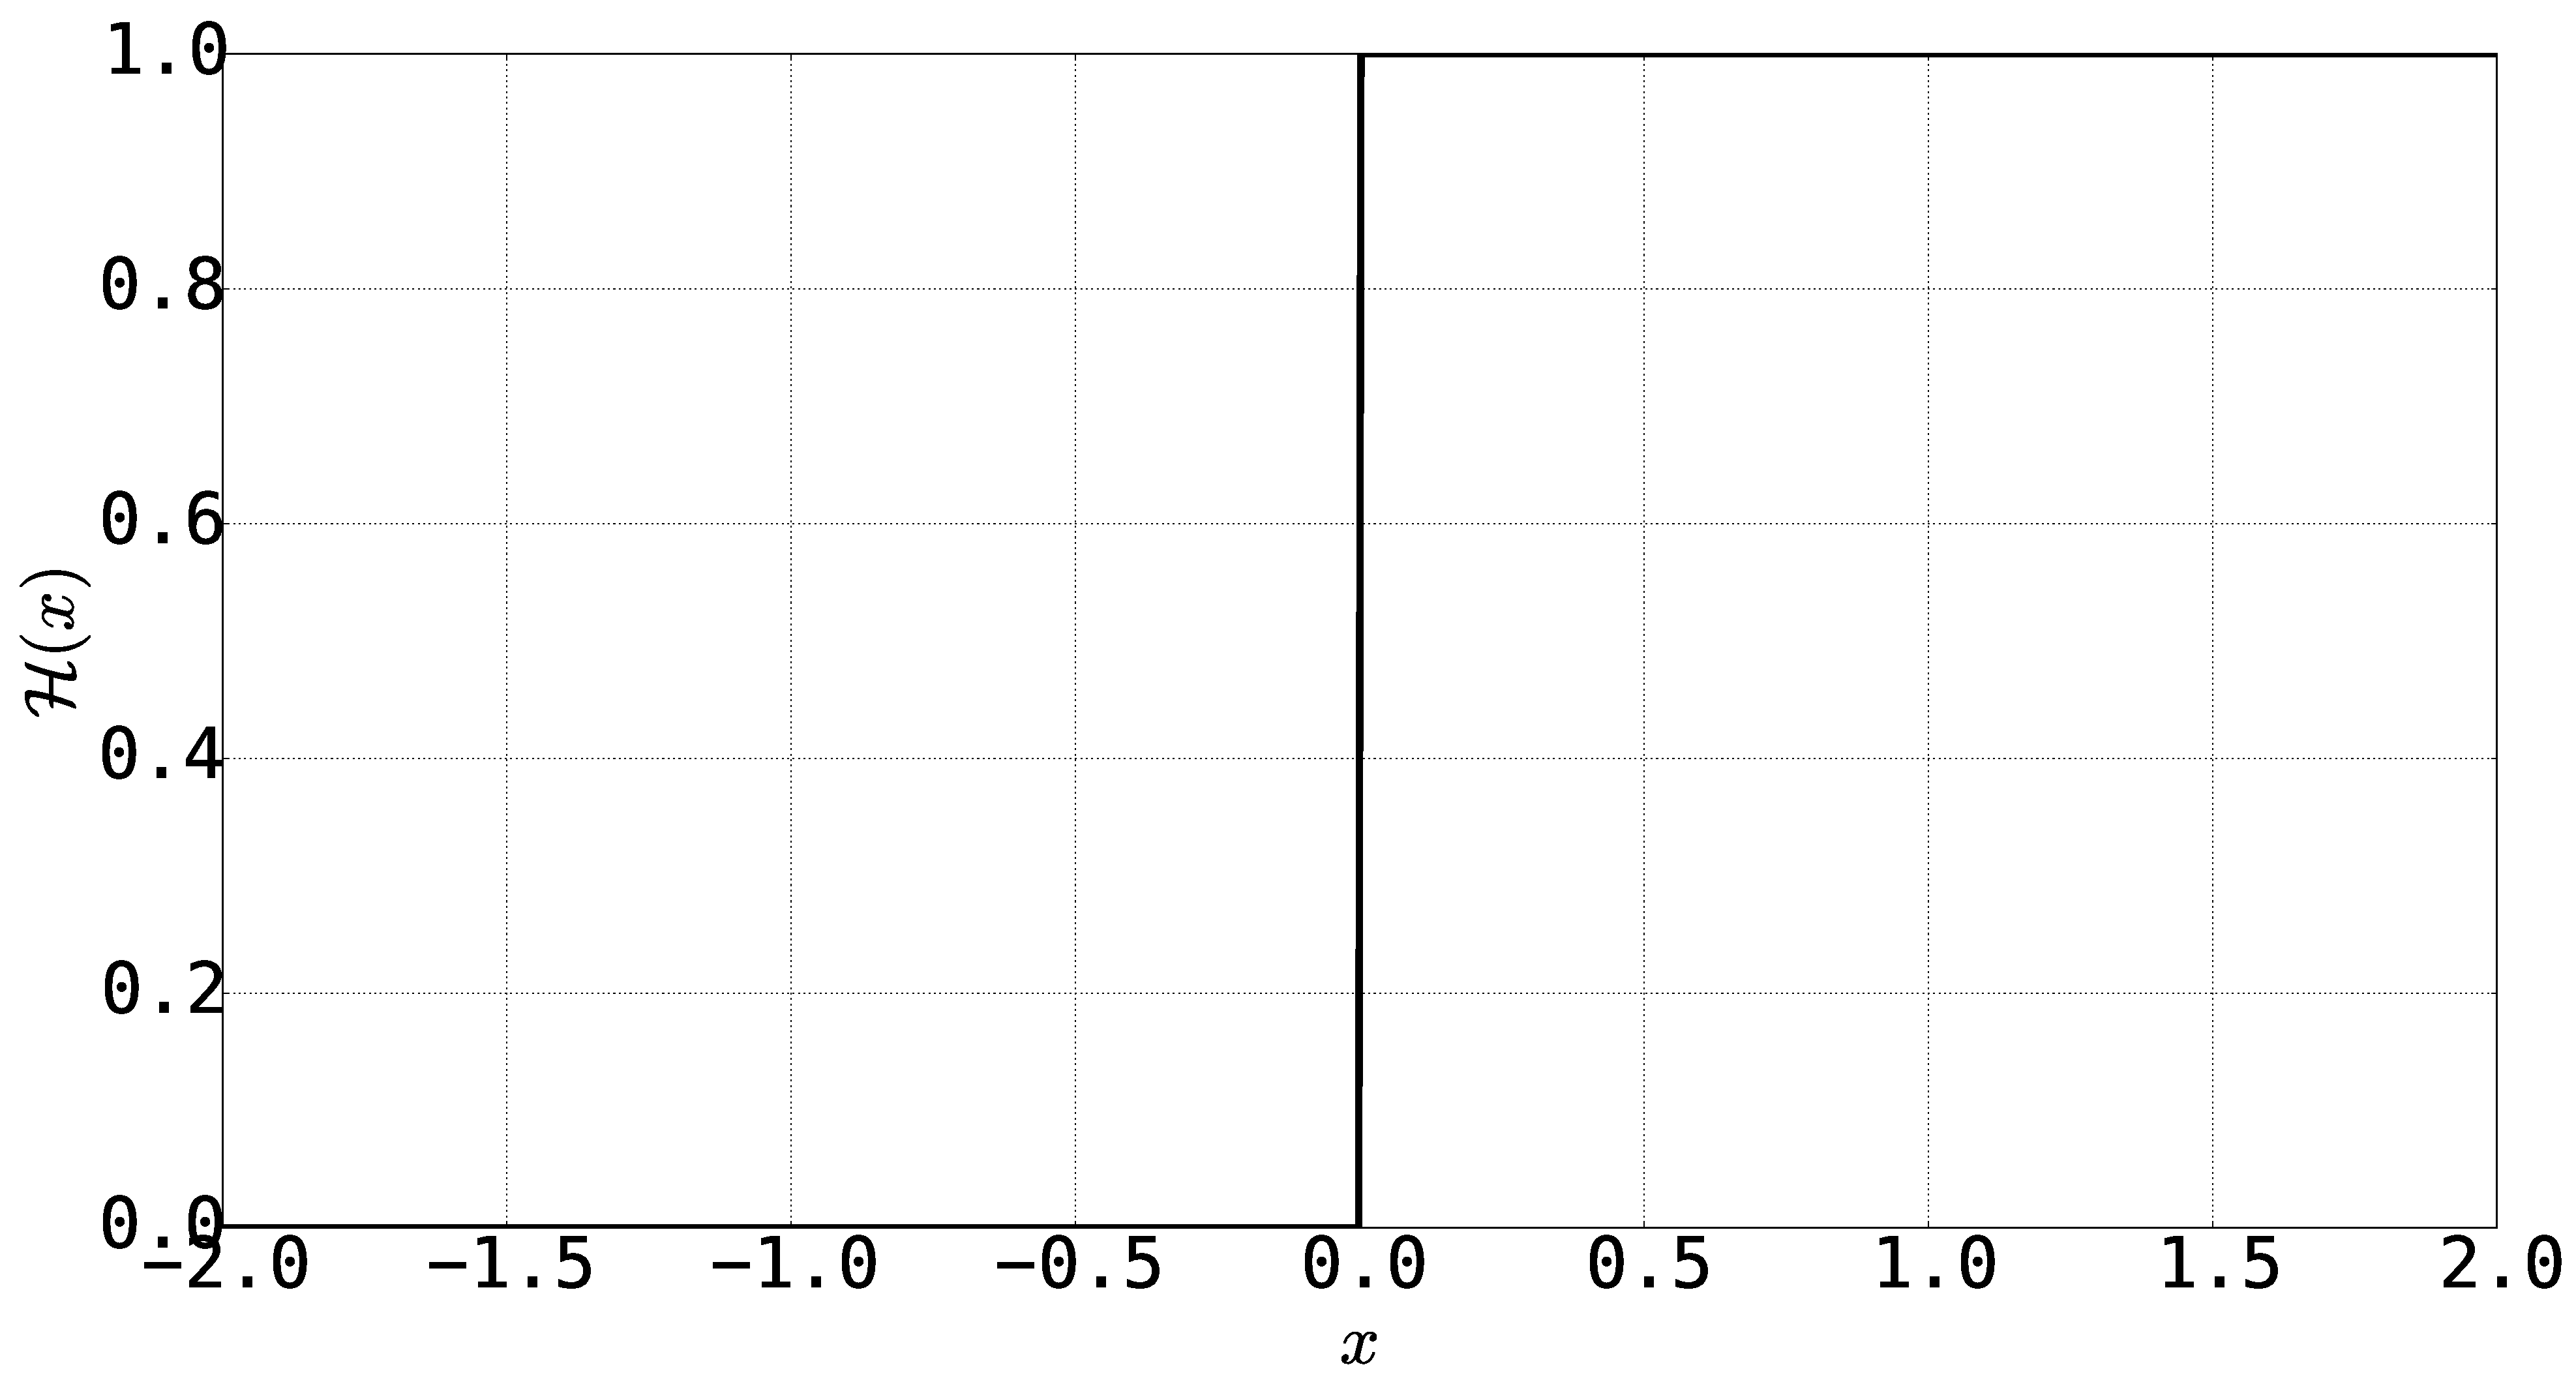
\includegraphics[width=14.cm]{Chapter_3/figure/Heaviside_Function.eps}
	\caption{The Heaviside function.}
	\label{{fig:C3_heavisideFunction}}
\end{figure}

By feeding the function $\mathcal{X}$ into the Heaviside function, we get the value of one for nodes inside the solid boundary and zero for outside. These are then multiplied to the force terms calculated using Equation \eqref{eq:C3_forceTermIBpenelization}. This enables us to apply the force term only within the solid domain. This method is applied to the demonstration problem of section \ref{sec:C3_benchmark_case}. For this problem, we looked at the effect of the number of mesh cells, wall velocity, and the permeability value on the accuracy of the method. The results are compared with analytical results for this problem like the previous sections.

For the first set of results, we looked at the effect of mesh size on the accuracy of the solution. The domain length is chosen as $1.0 m$ where the position of the fixed wall is selected as $0.6125$. We chose this so that the computational nodes won't coincide the with the wall location. This better represents the application of the IB method. We chose the node numbers as 11, 41, 81, and 161. As shown in Figure \ref{fig:C3_penalizationResultNodeNumber}, as we increase the number of the total error between the numerical and analytical results decreases. For the Case where there is computational node exactly on top the location for the stationary wall ($n=161$), the two results match perfectly. The IB results are shown using solid line and the analytical results are represented using white circles.

\begin{figure}[H]
	\centering
	\subfigure[n = 11]
	{
	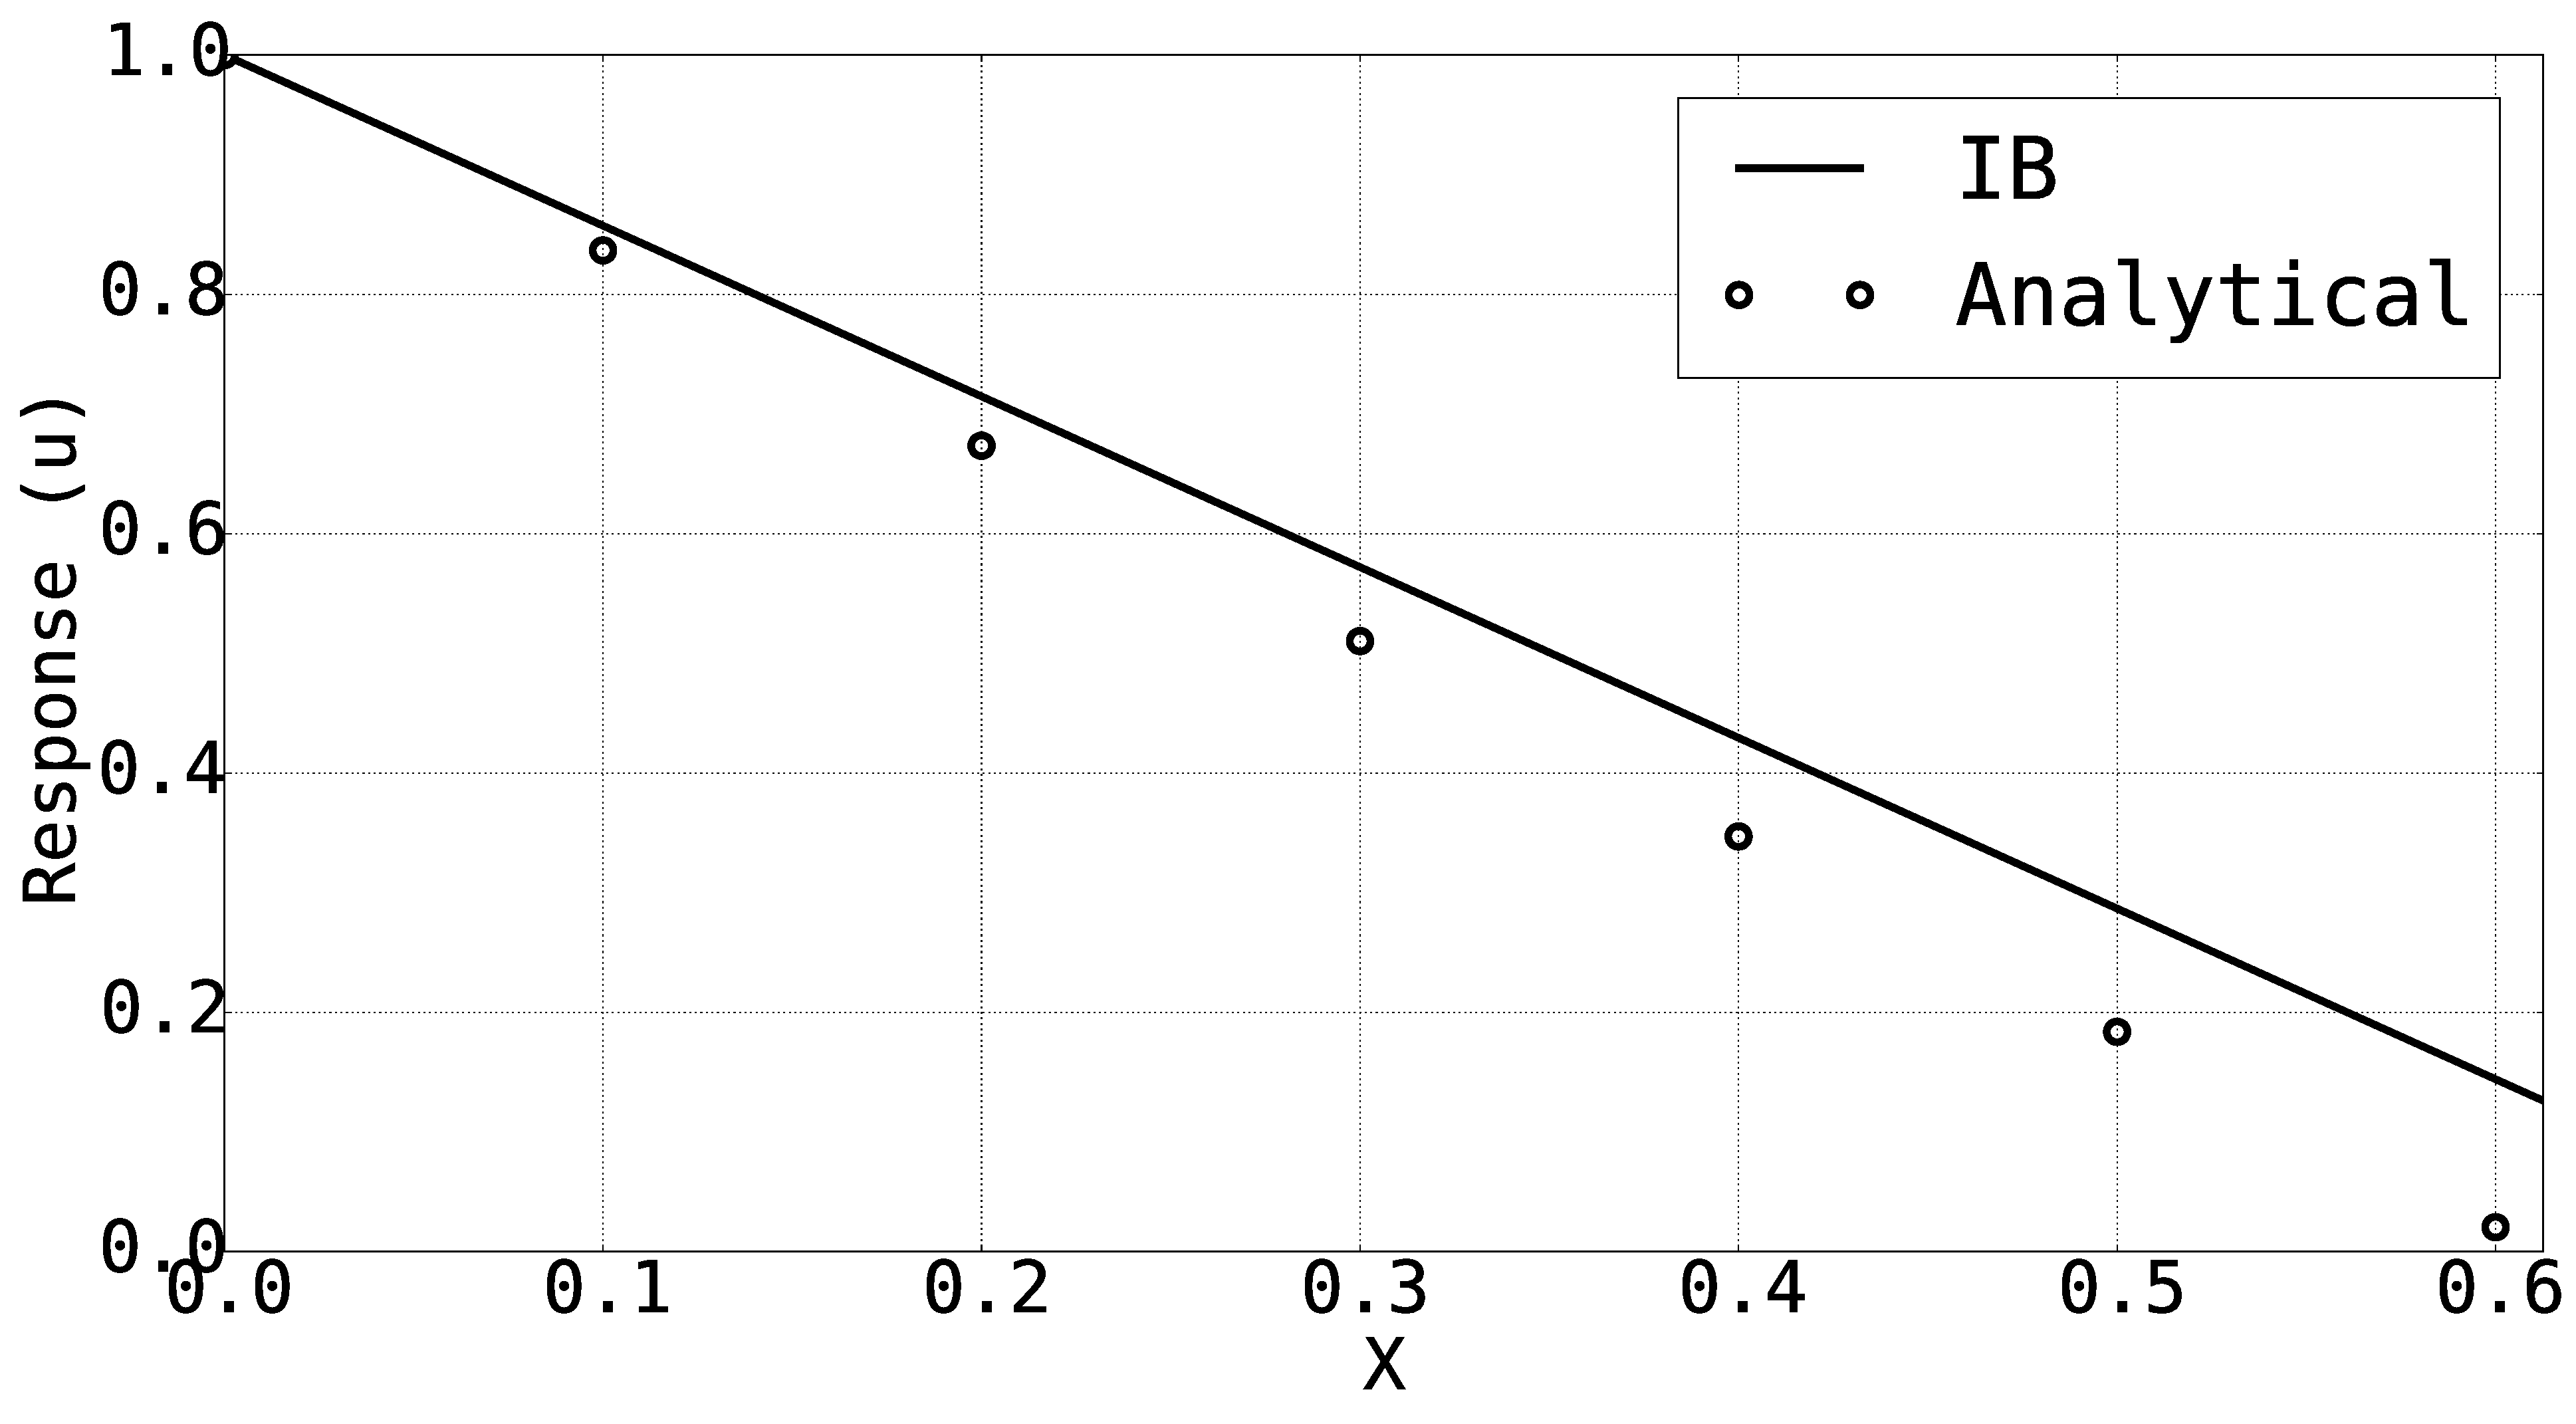
\includegraphics[width=7.0cm]{Chapter_3/figure/penalization_nodeNumber_11.eps}
	}
	\quad
	\subfigure[n = 41]
	{
	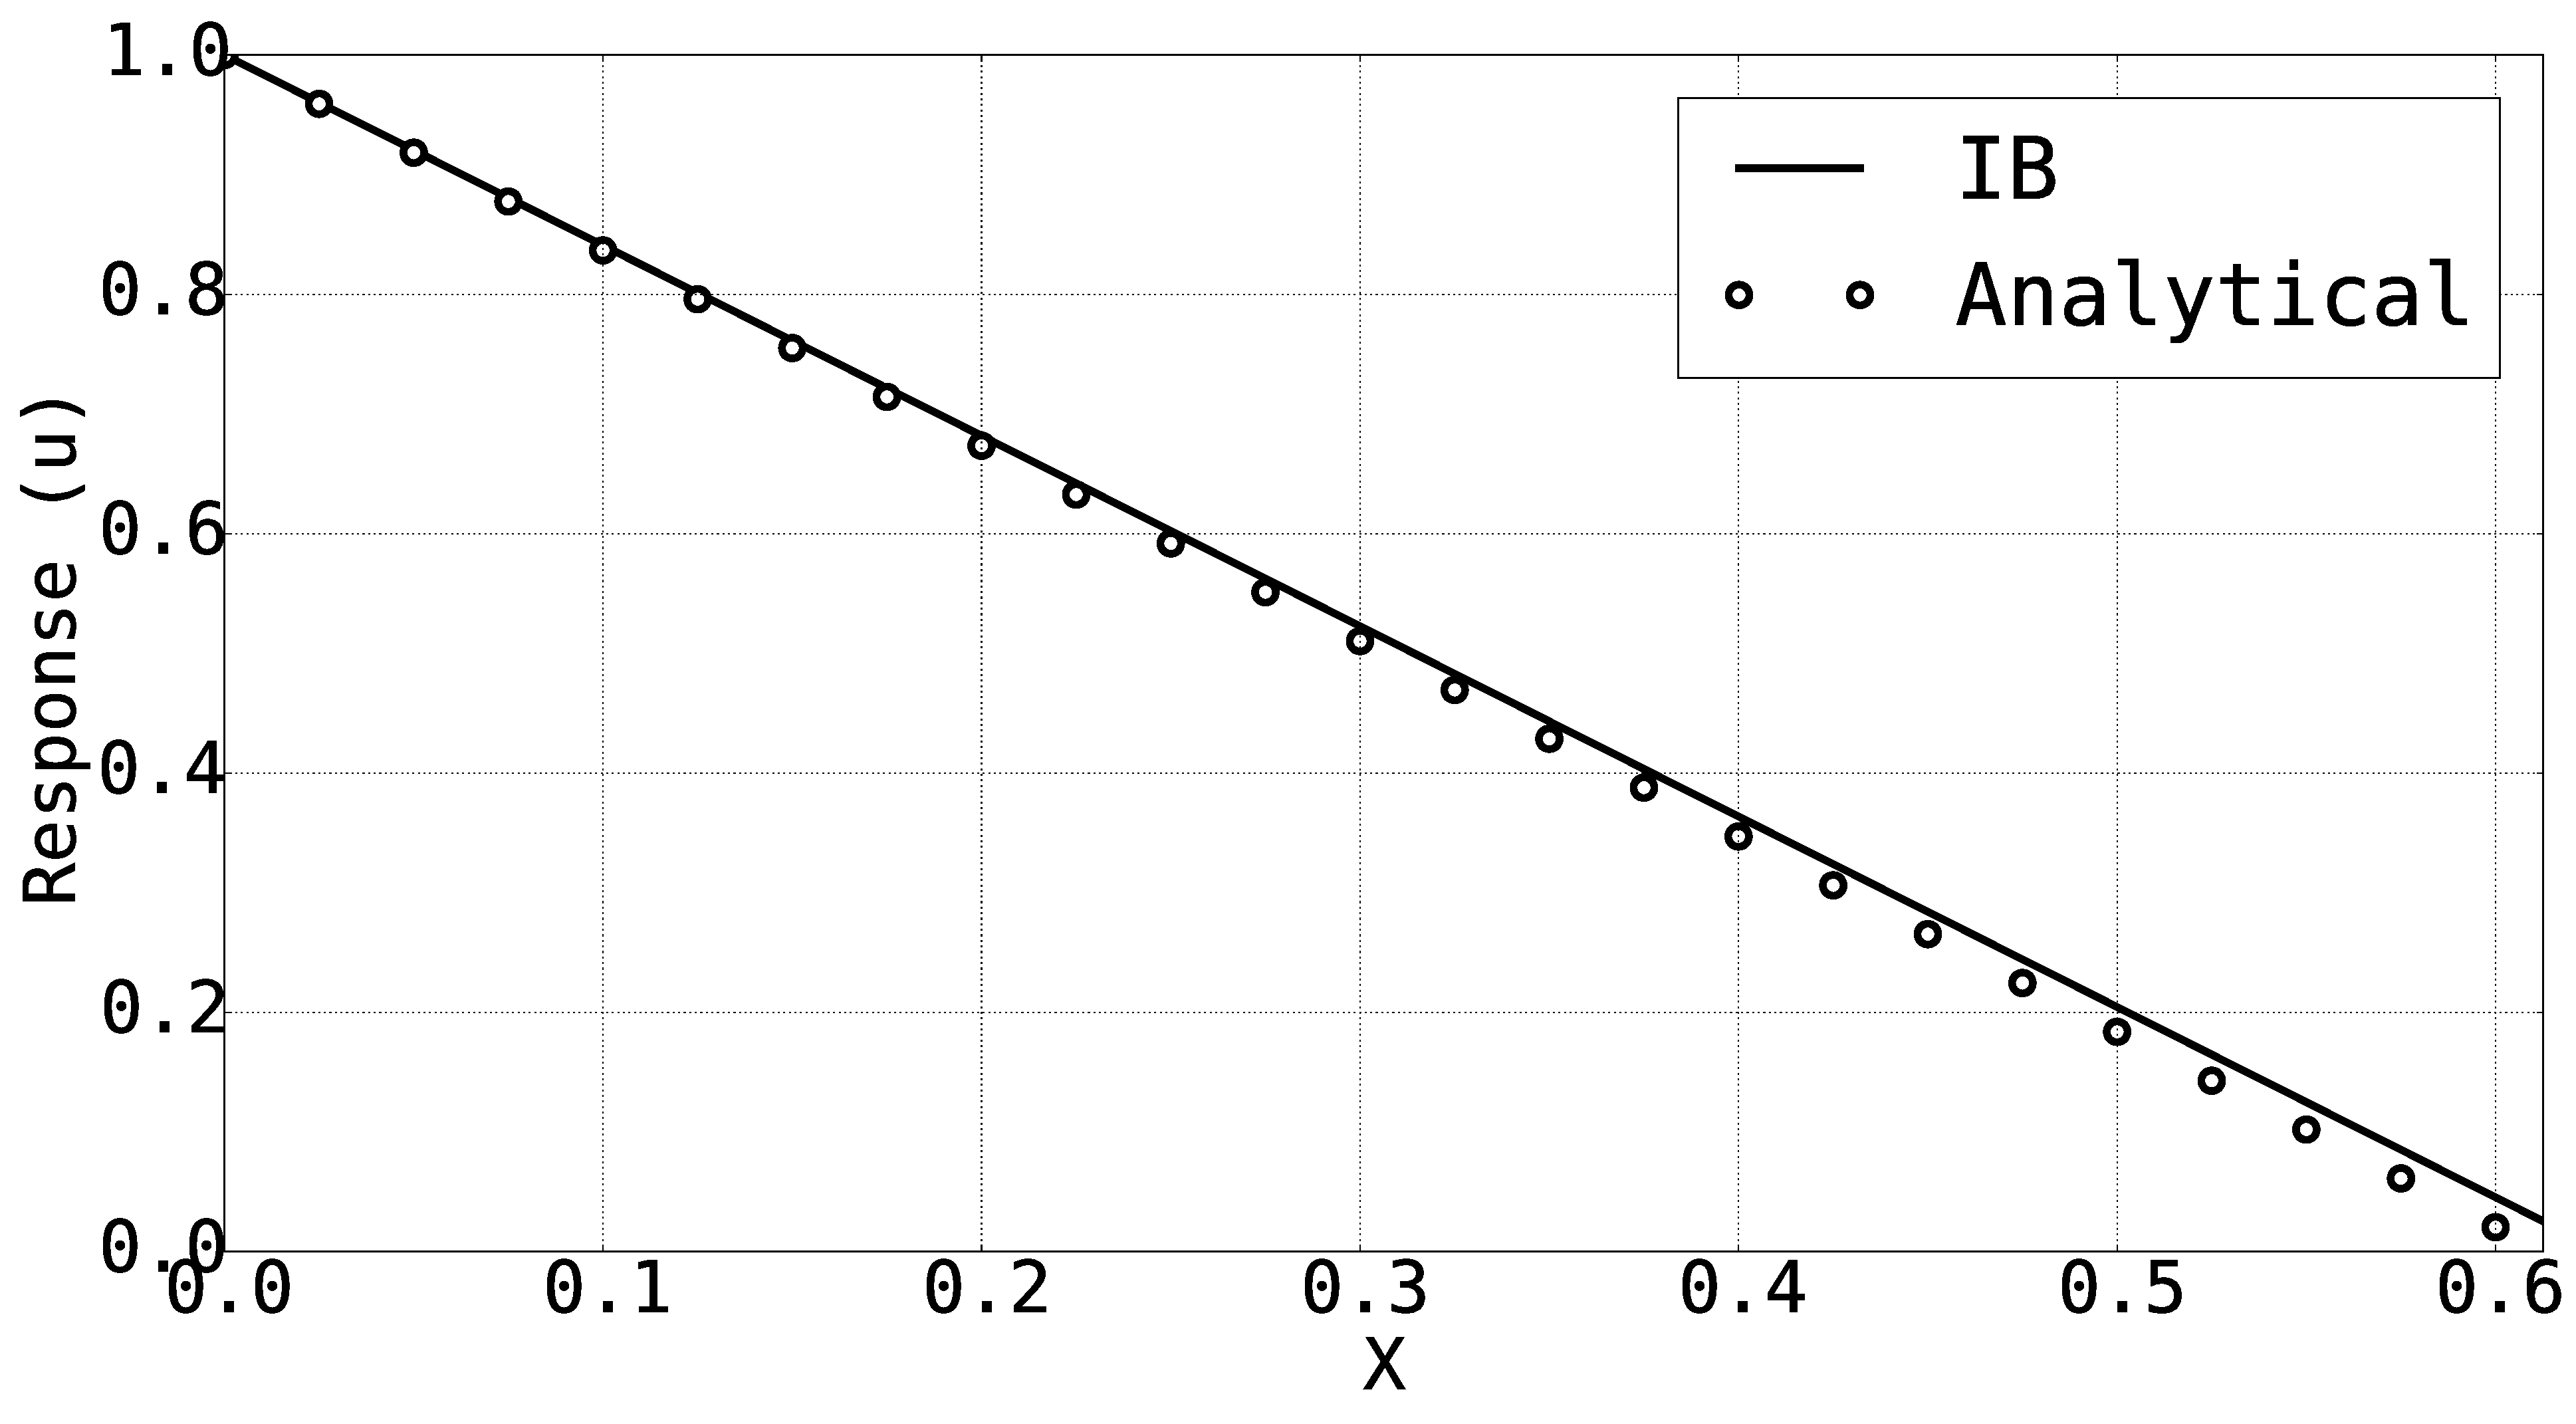
\includegraphics[width=7.0cm]{Chapter_3/figure/penalization_nodeNumber_41.eps}
	}
	\\
	\subfigure[n = 81]
	{
	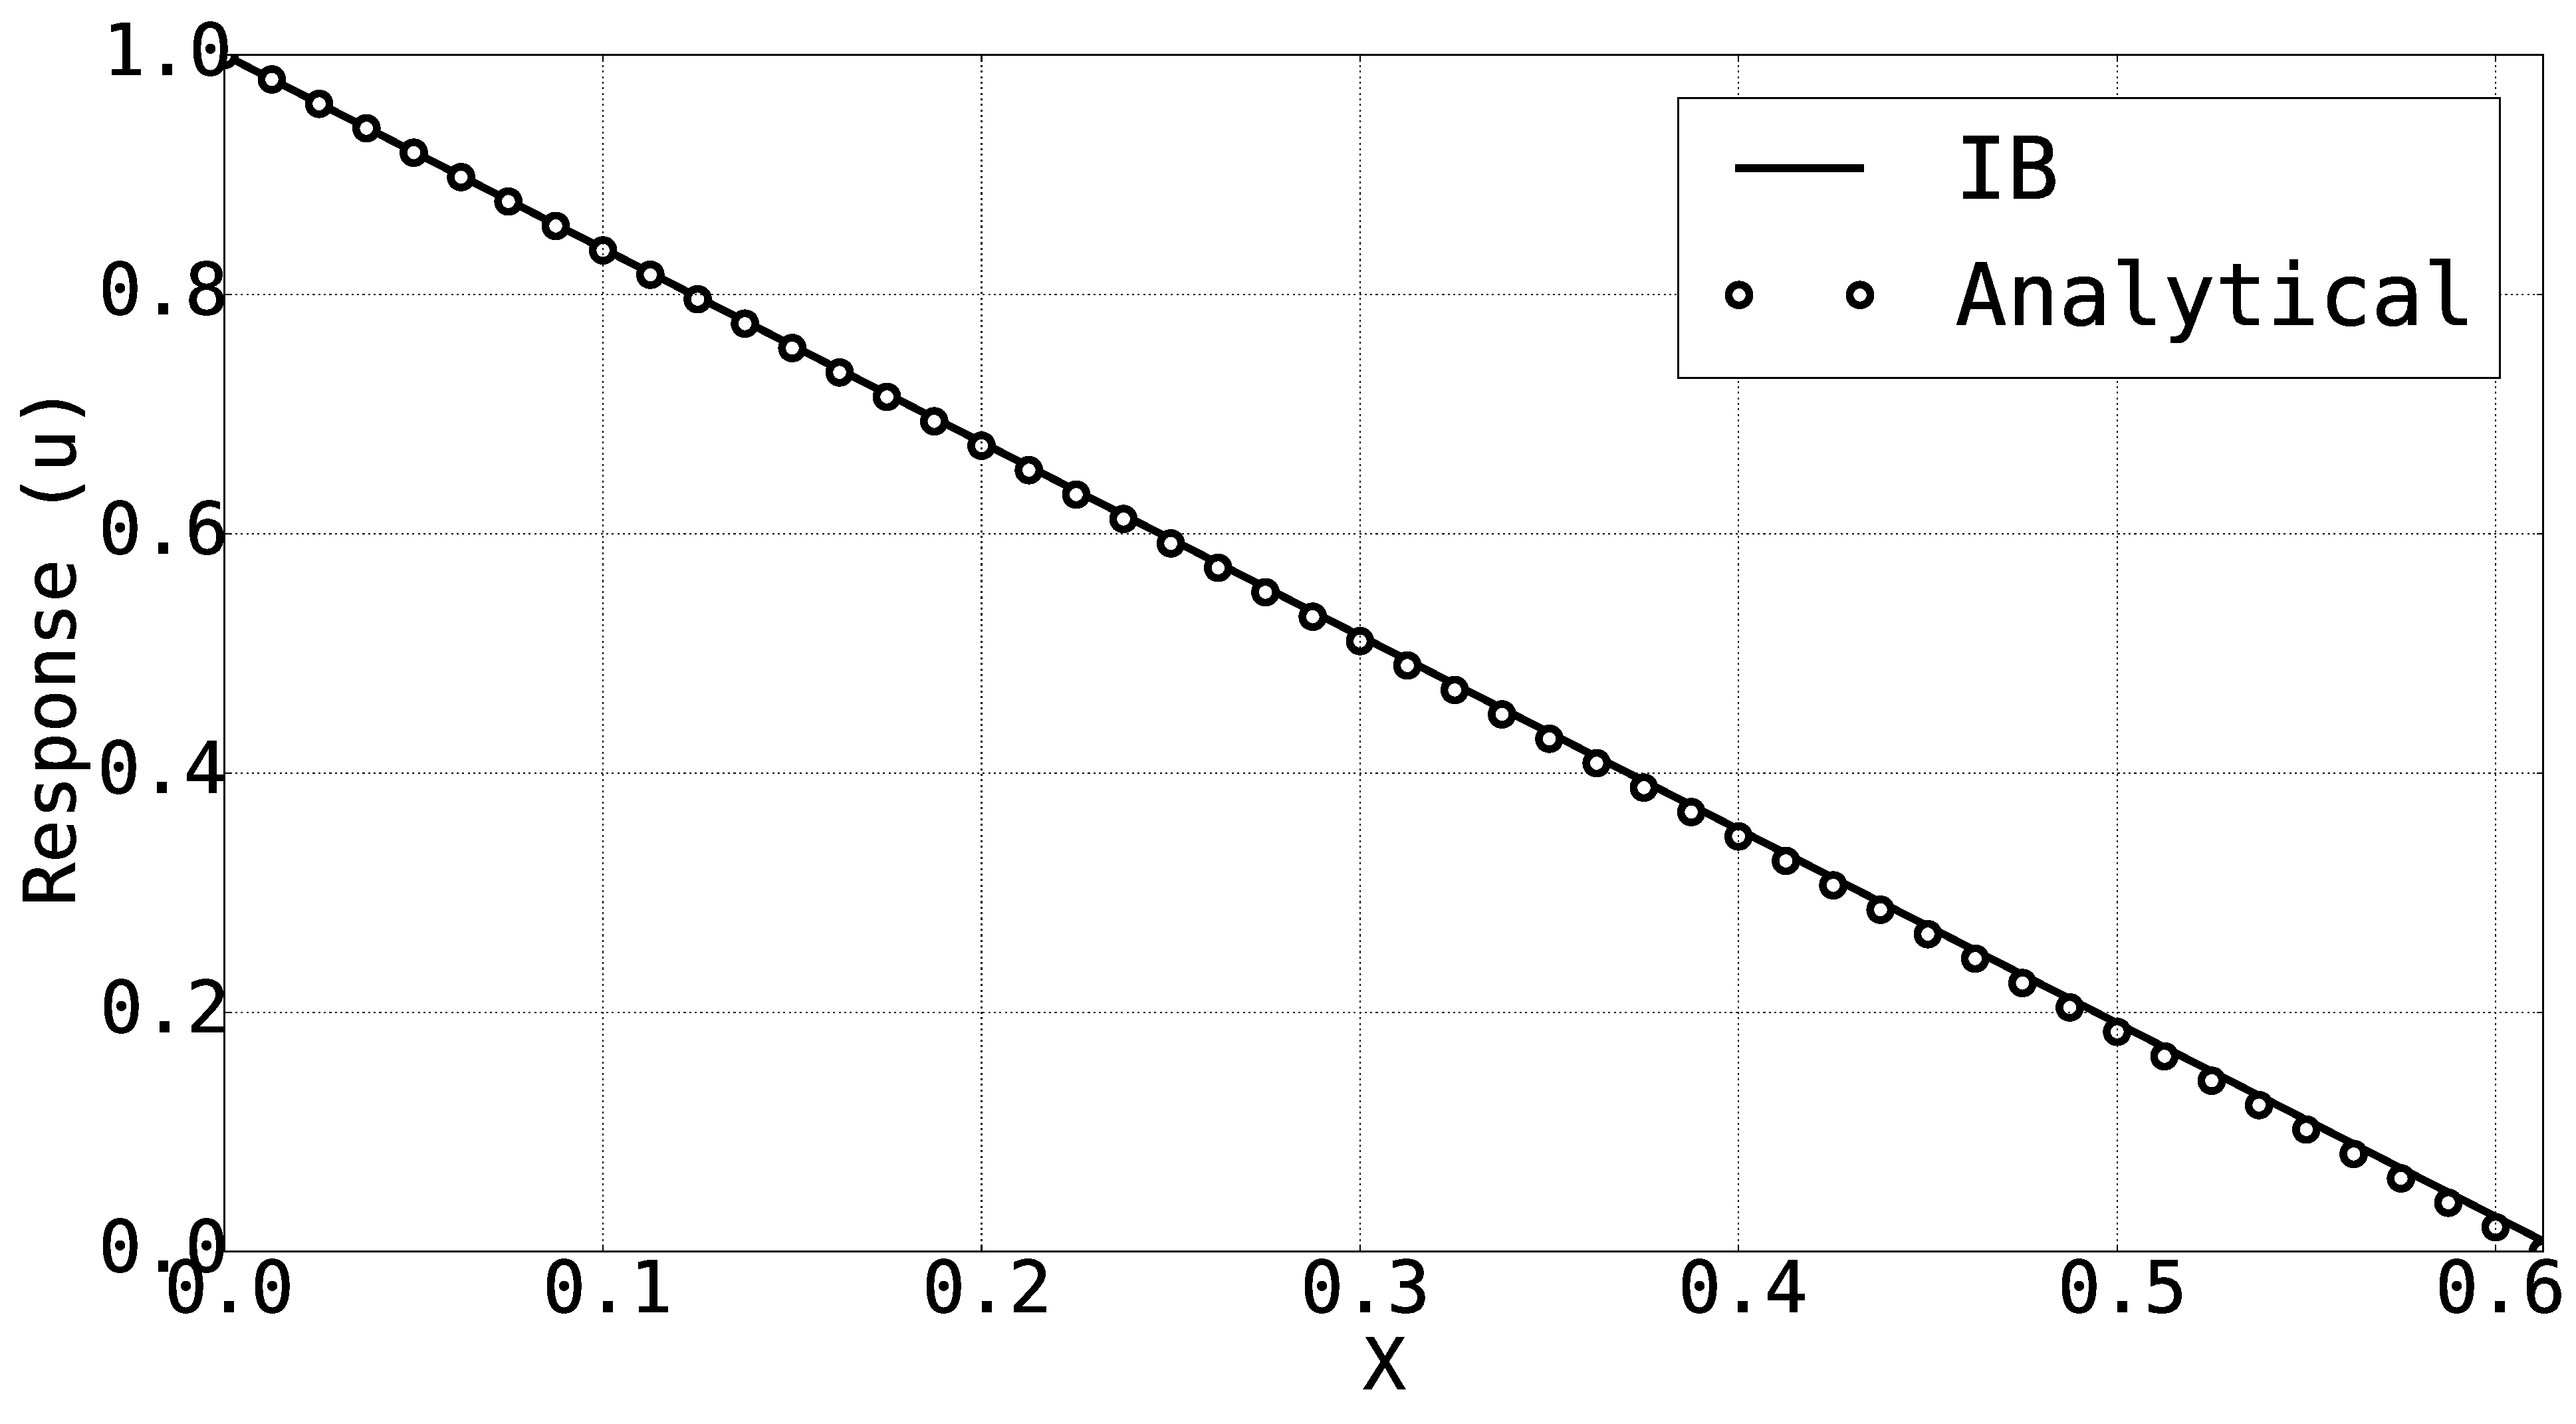
\includegraphics[width=7.0cm]{Chapter_3/figure/penalization_nodeNumber_81.eps}
	}
	\quad
	\subfigure[n = 161]
	{
	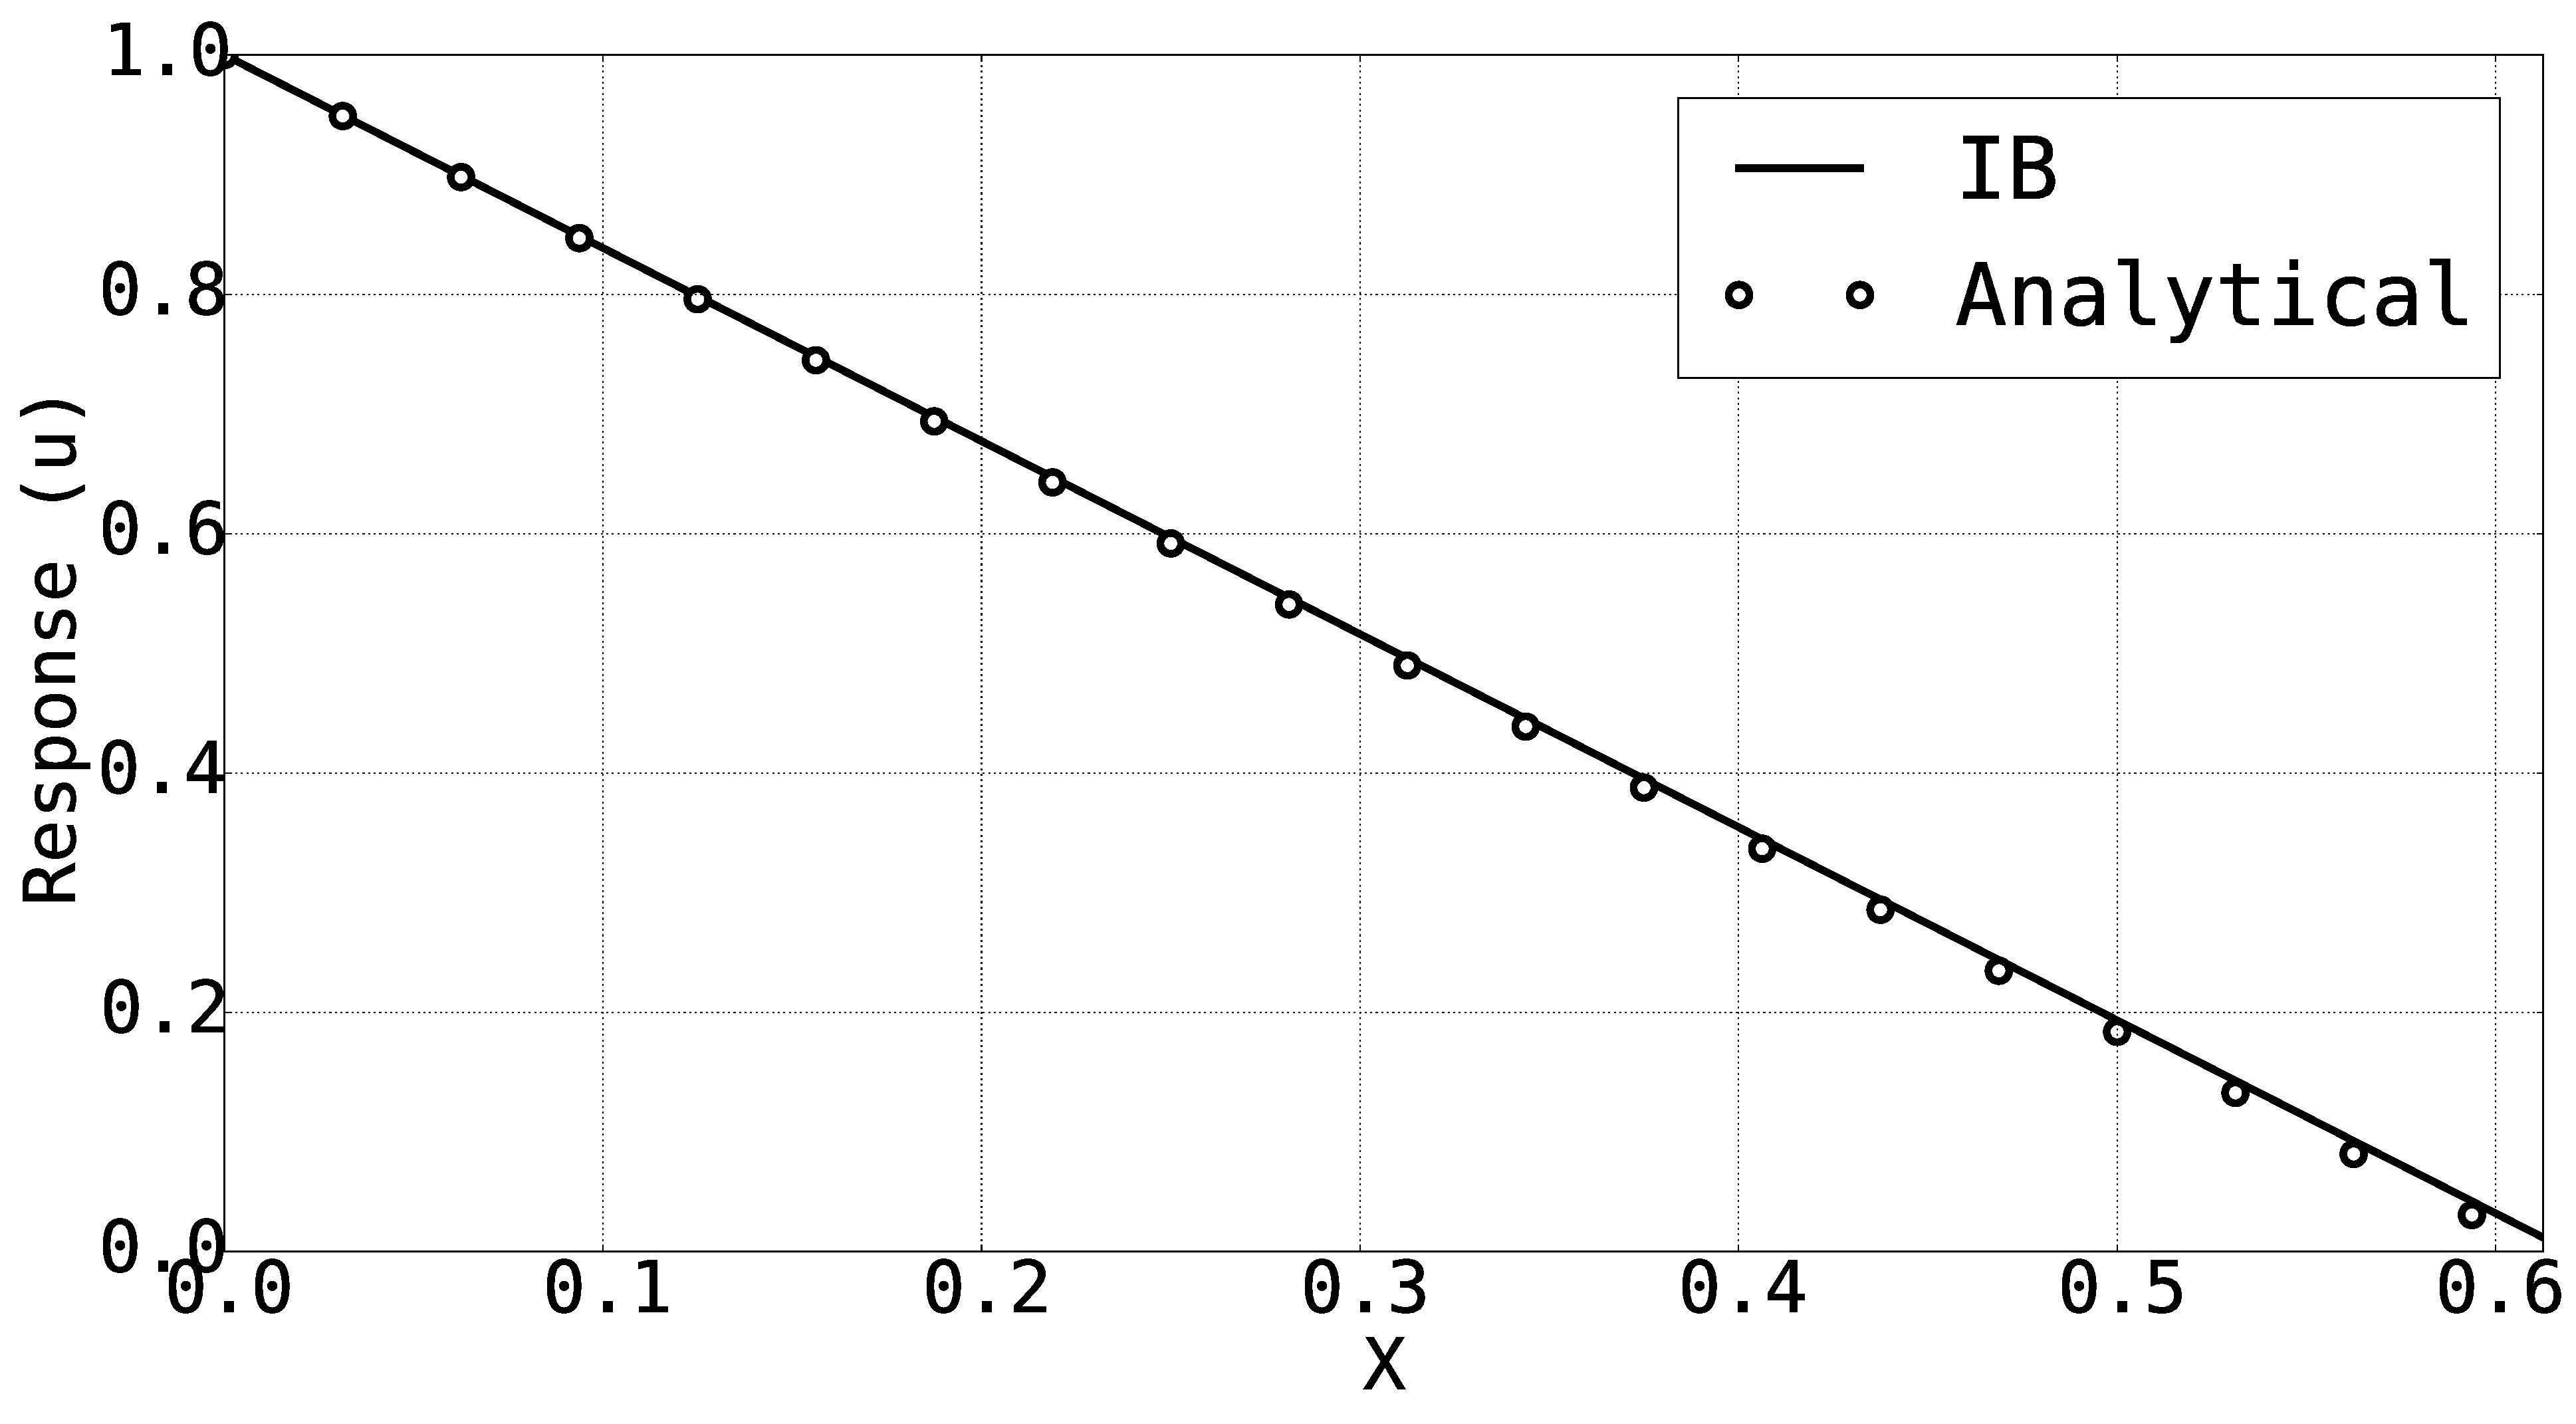
\includegraphics[width=7.0cm]{Chapter_3/figure/penalization_nodeNumber_161.eps}
	}
	\caption{Comparison between IB and analytical results for different number of nodes.}
	\label{fig:C3_penalizationResultNodeNumber}
\end{figure}

For the comparison between the IB and the analytical results we used the RSME value. These are shown in Table \ref{table:C3_penalizationResultNodeNumberRMSE}.

\begin{table}[H]
\centering
\begin{tabular}{c | c}
	Node number & RMSE value \\ \hline \hline
	11 & 0.0624 \\ \hline
	41 & 0.0139 \\ \hline
	81 & 0.005 \\ \hline
	161 & 0.001
\end{tabular}
\caption{RMSE value for different number of nodes}
\label{table:C3_penalizationResultNodeNumberRMSE}
\end{table}

As can be seen in Table \ref{table:C3_penalizationResultNodeNumberRMSE}, even for $n = 161$, the RMSE value is not zero. This is because in the penalization method, even for low values of porosity, there is still a small flow going through the solid domain.

For the next investigation, we look at the effect of the different velocity of moving wall on the accuracy of the penalization method. For this analysis we defined the fixed wall at $x=0.4325$ and discretized the domain using $81$ nodes. The inlet velocity is selected as $1$, $10$, $100$, and $1000$. To verify the methodology, we compared the IB with analytical results. We chose the time step as $10^{-5}$ and the porosity value as $\kappa = 10^{-5}$. As shown in Figure \ref{fig:C3_penalizationResultInletVelocity} and the RMSE values in Table \ref{table:C3_penalizationResultInletVelocityRMSE}, the inlet velocity does not affect the the accuracy of the response. Moreover, all of these simulation are done using the same time step and porosity value.

\begin{figure}[H]
	\centering
	\subfigure[$U_{in} = 1 m/s$]
	{
	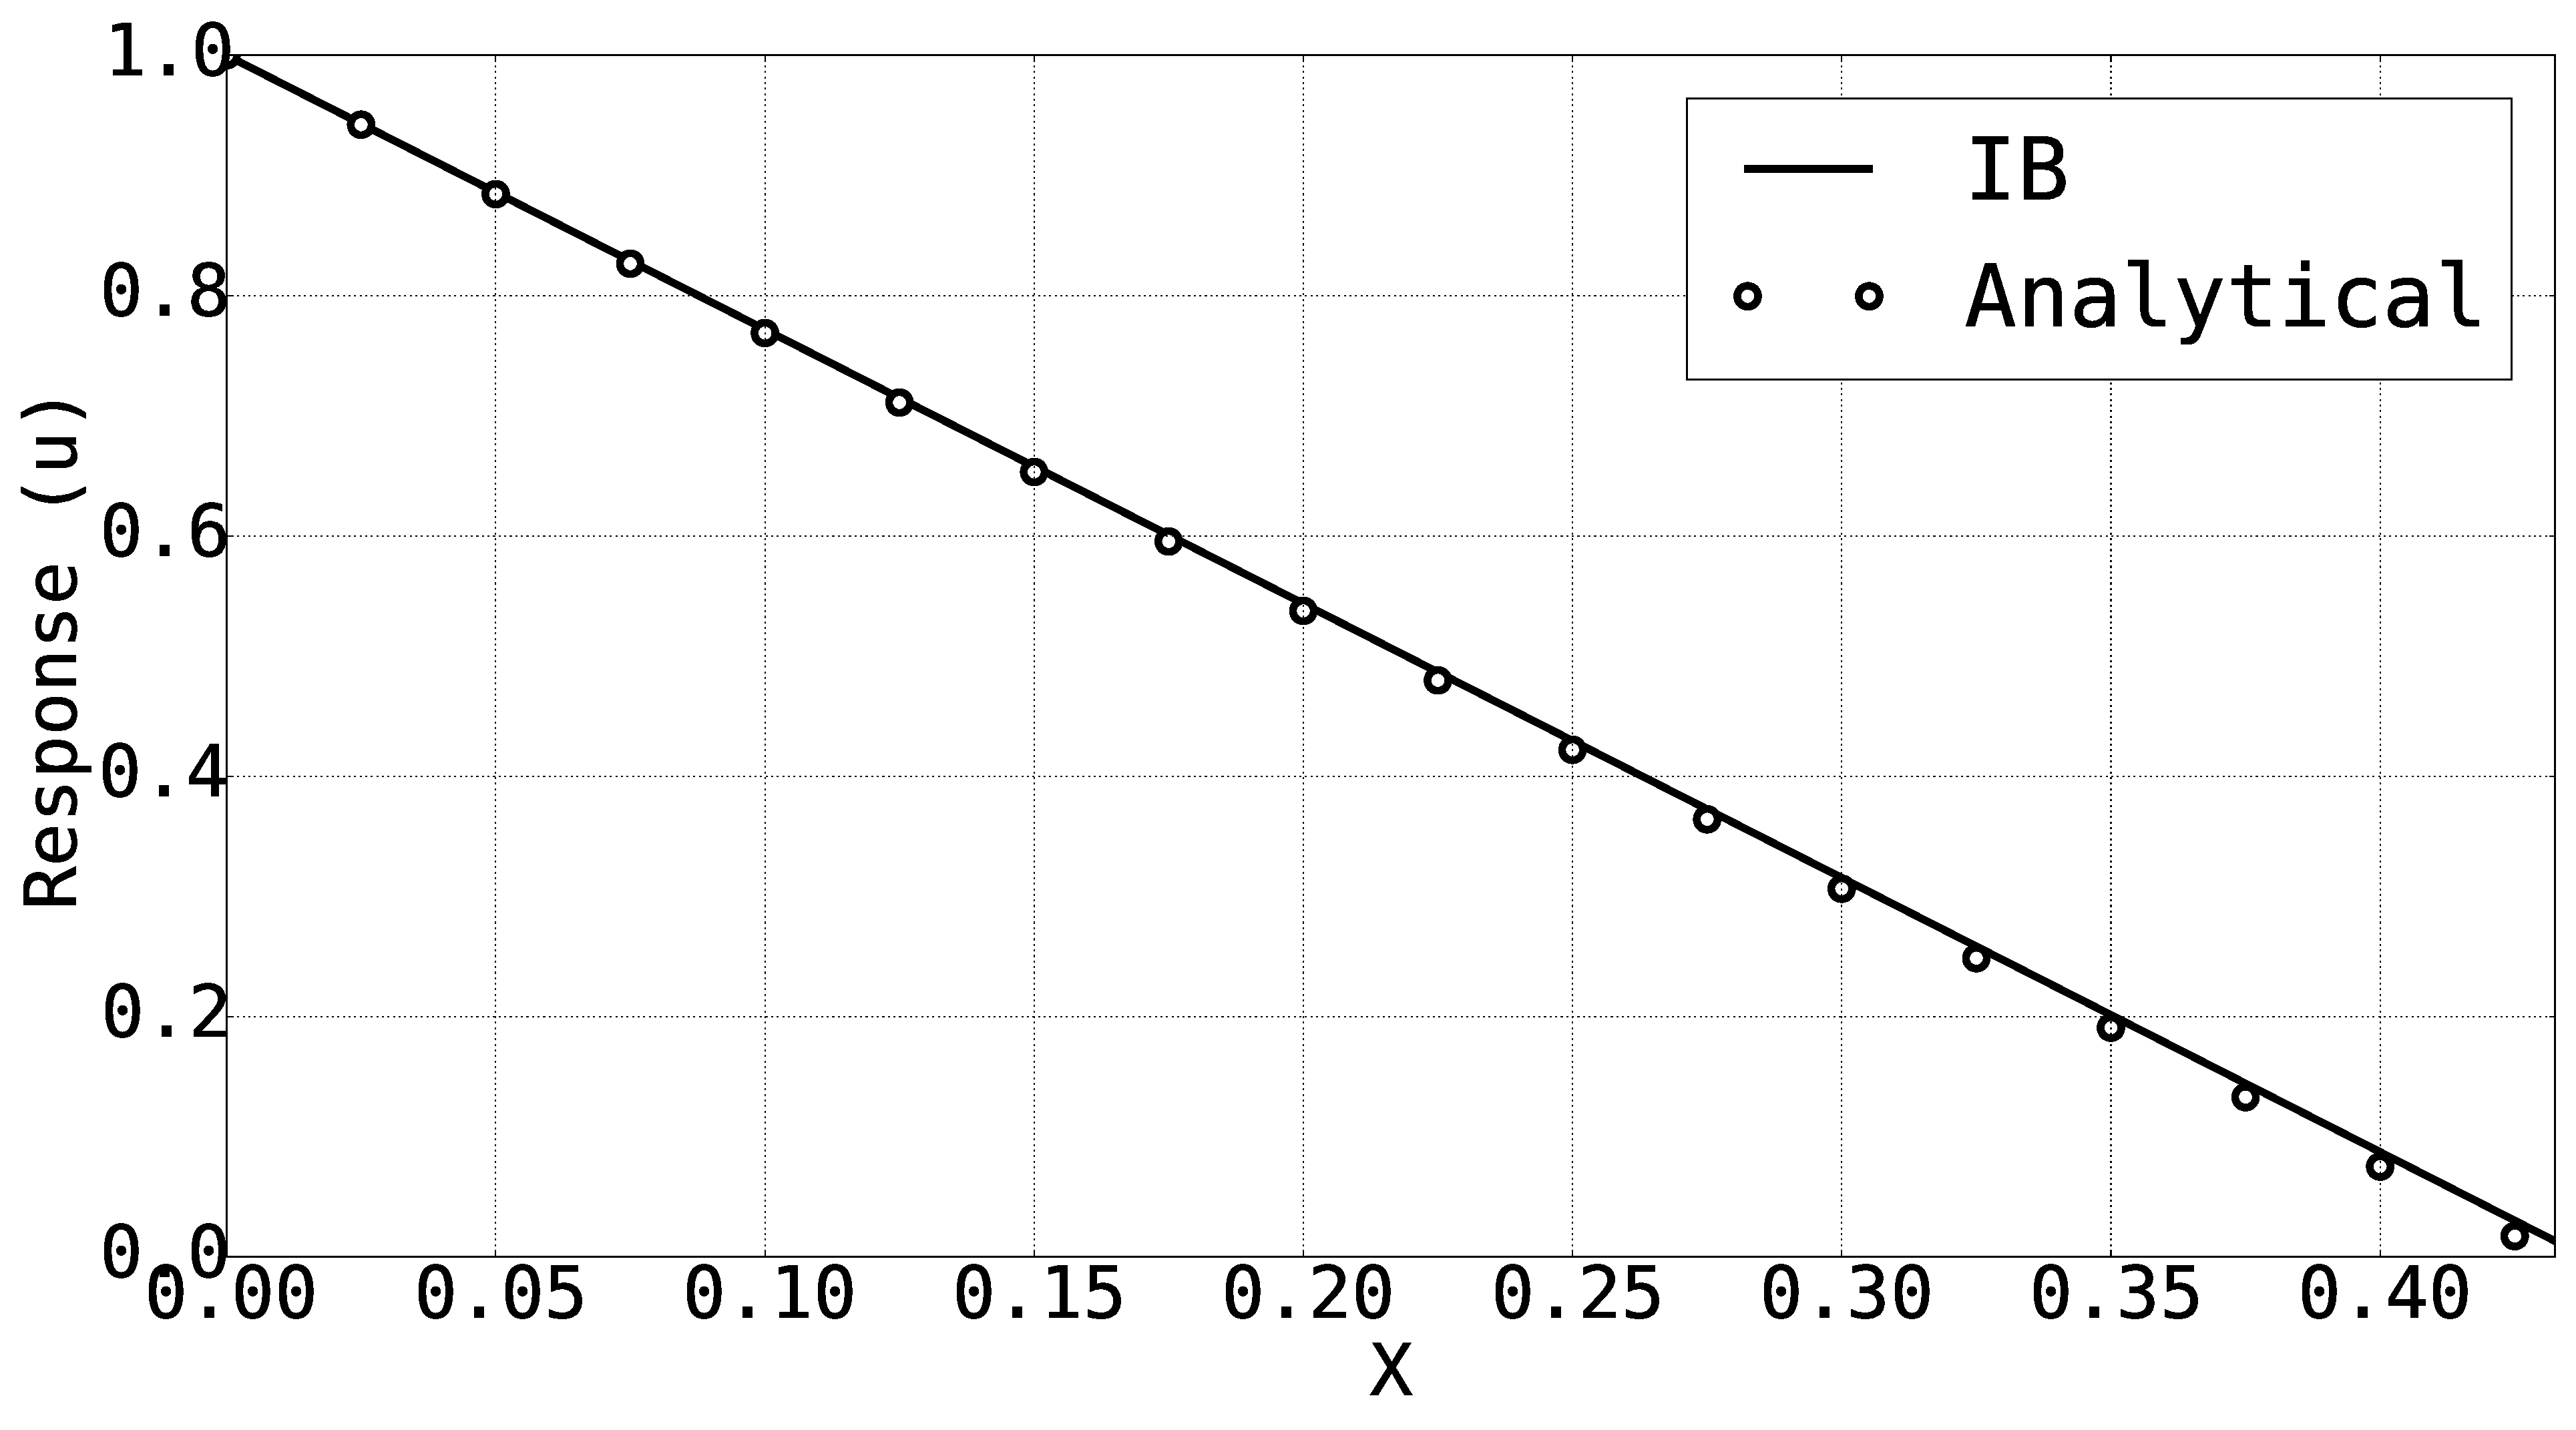
\includegraphics[width=7.0cm]{Chapter_3/figure/penalization_inletVelocity_1.eps}
	}
	\quad
	\subfigure[$U_{in} = 10 m/s$]
	{
	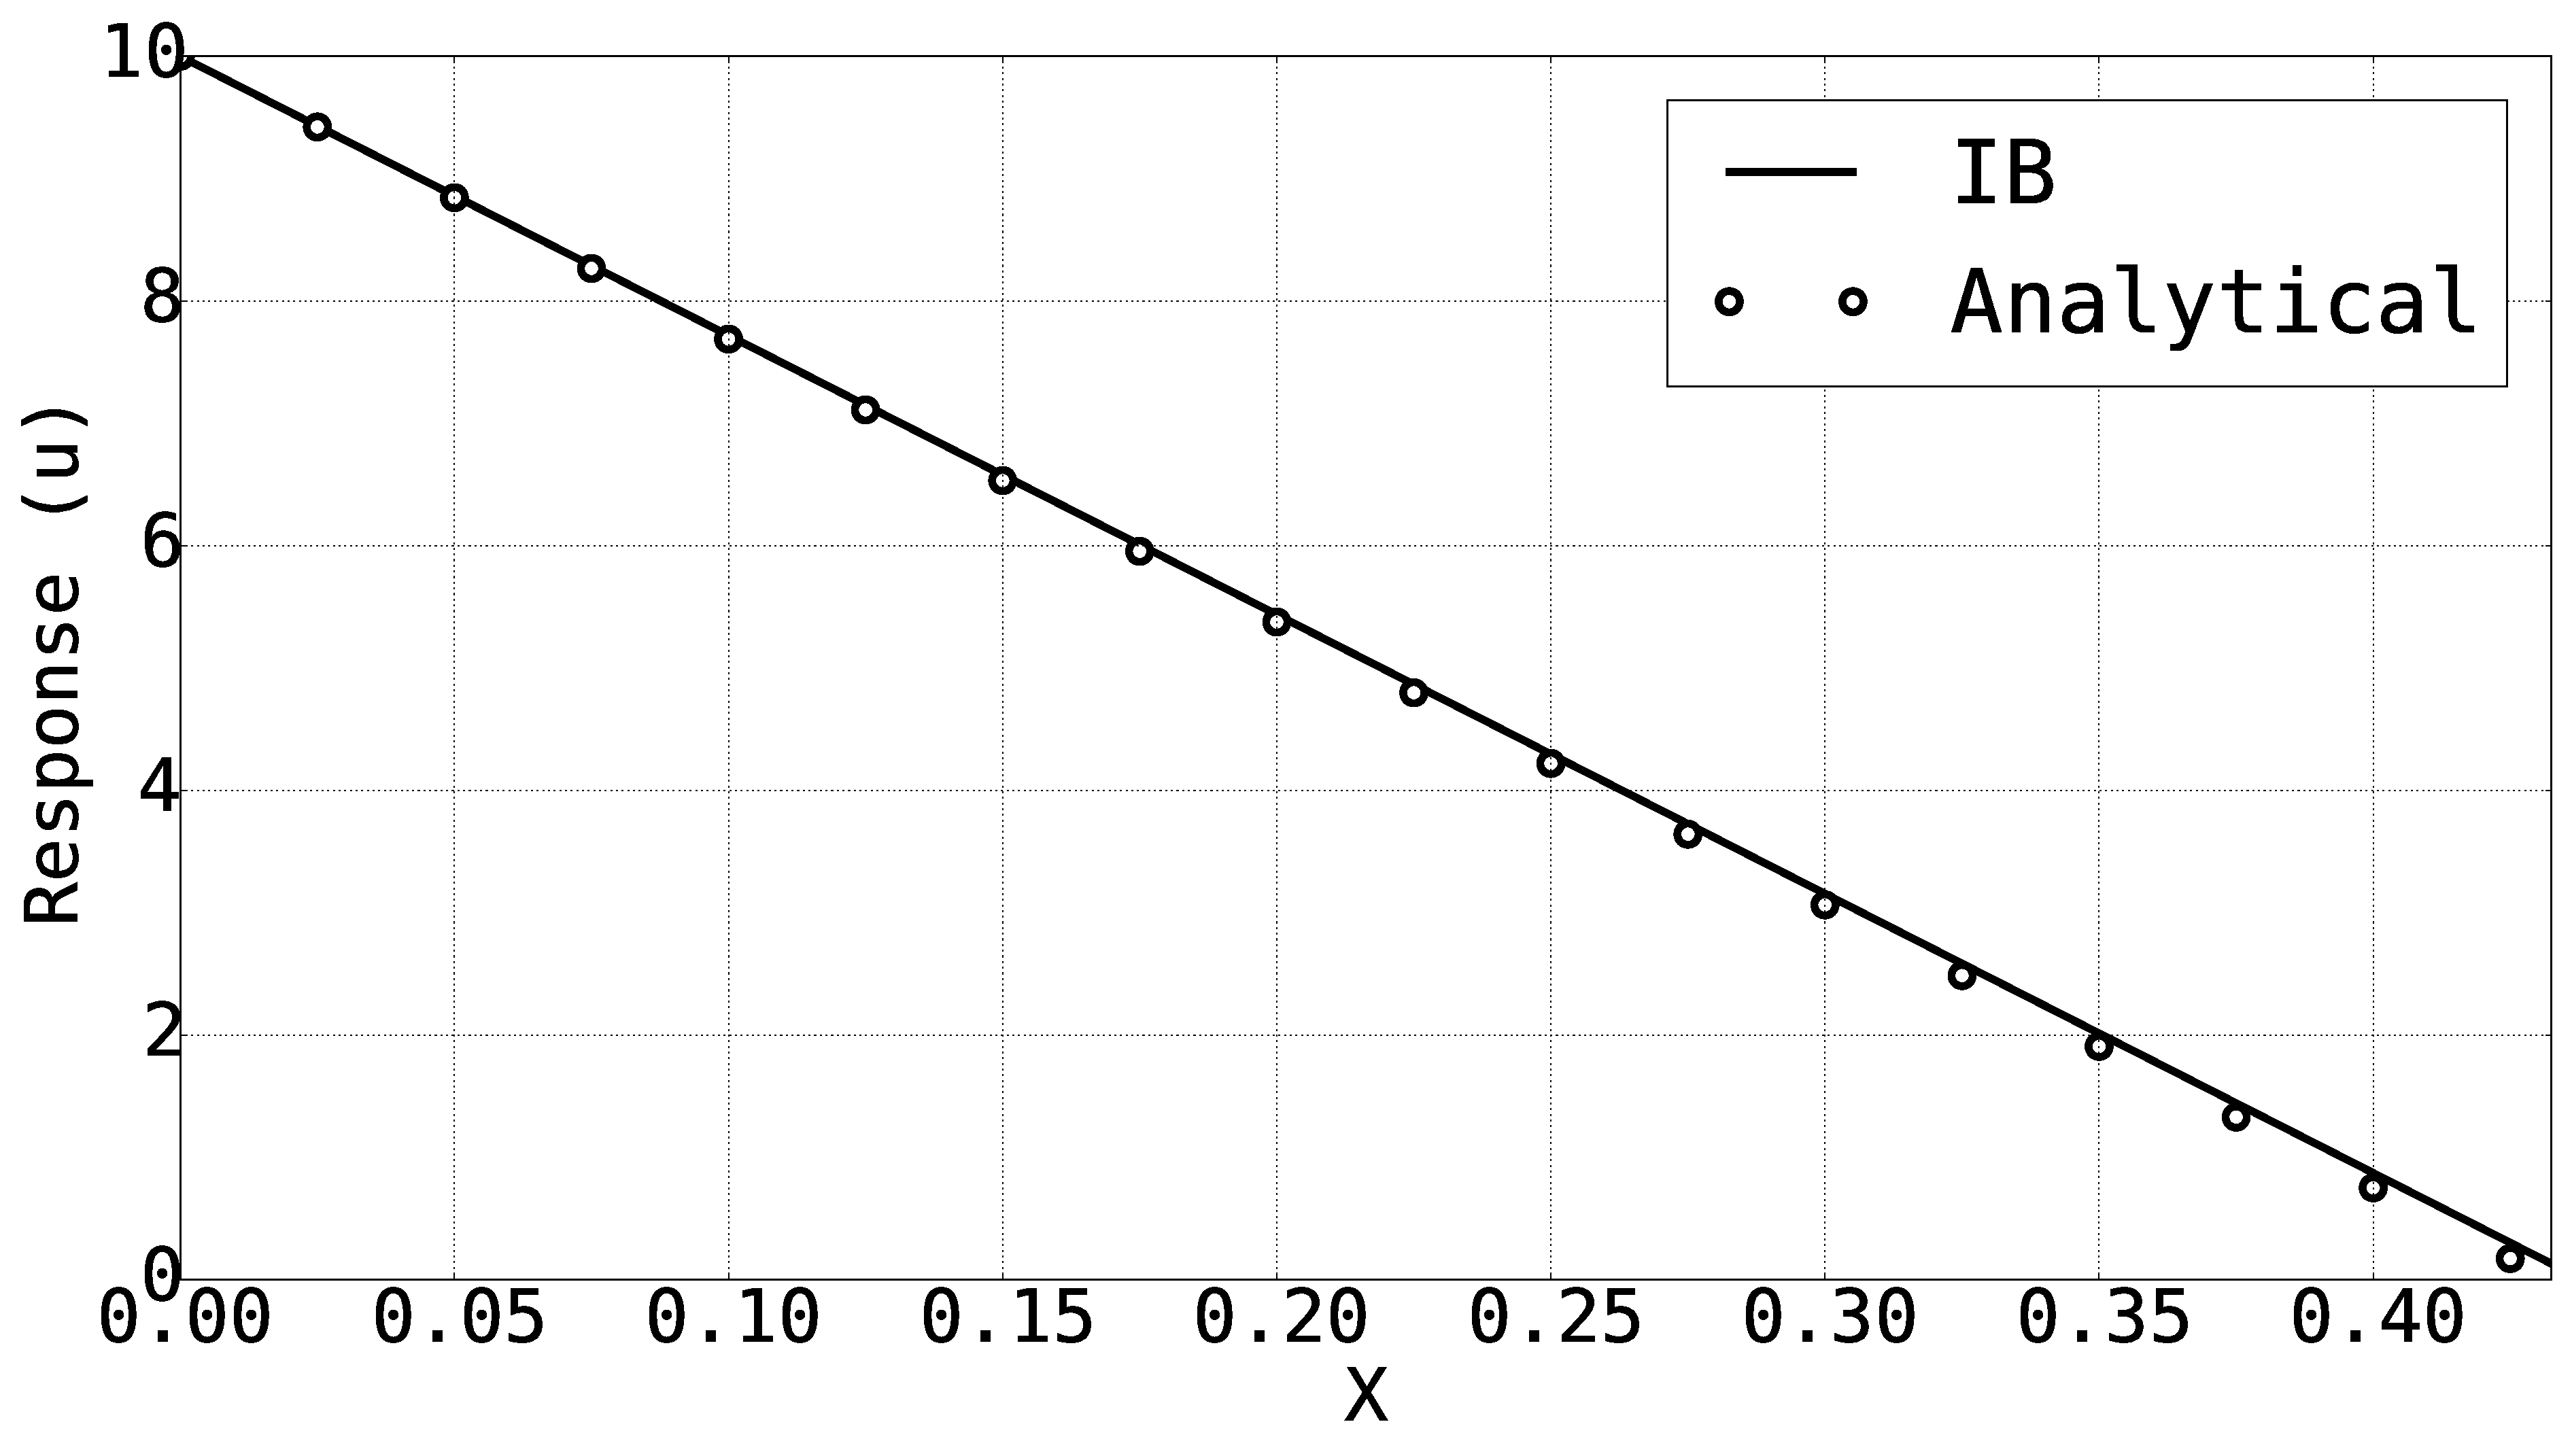
\includegraphics[width=7.0cm]{Chapter_3/figure/penalization_inletVelocity_10.eps}
	}
	\\
	\subfigure[$U_{in} = 100 m/s$]
	{
	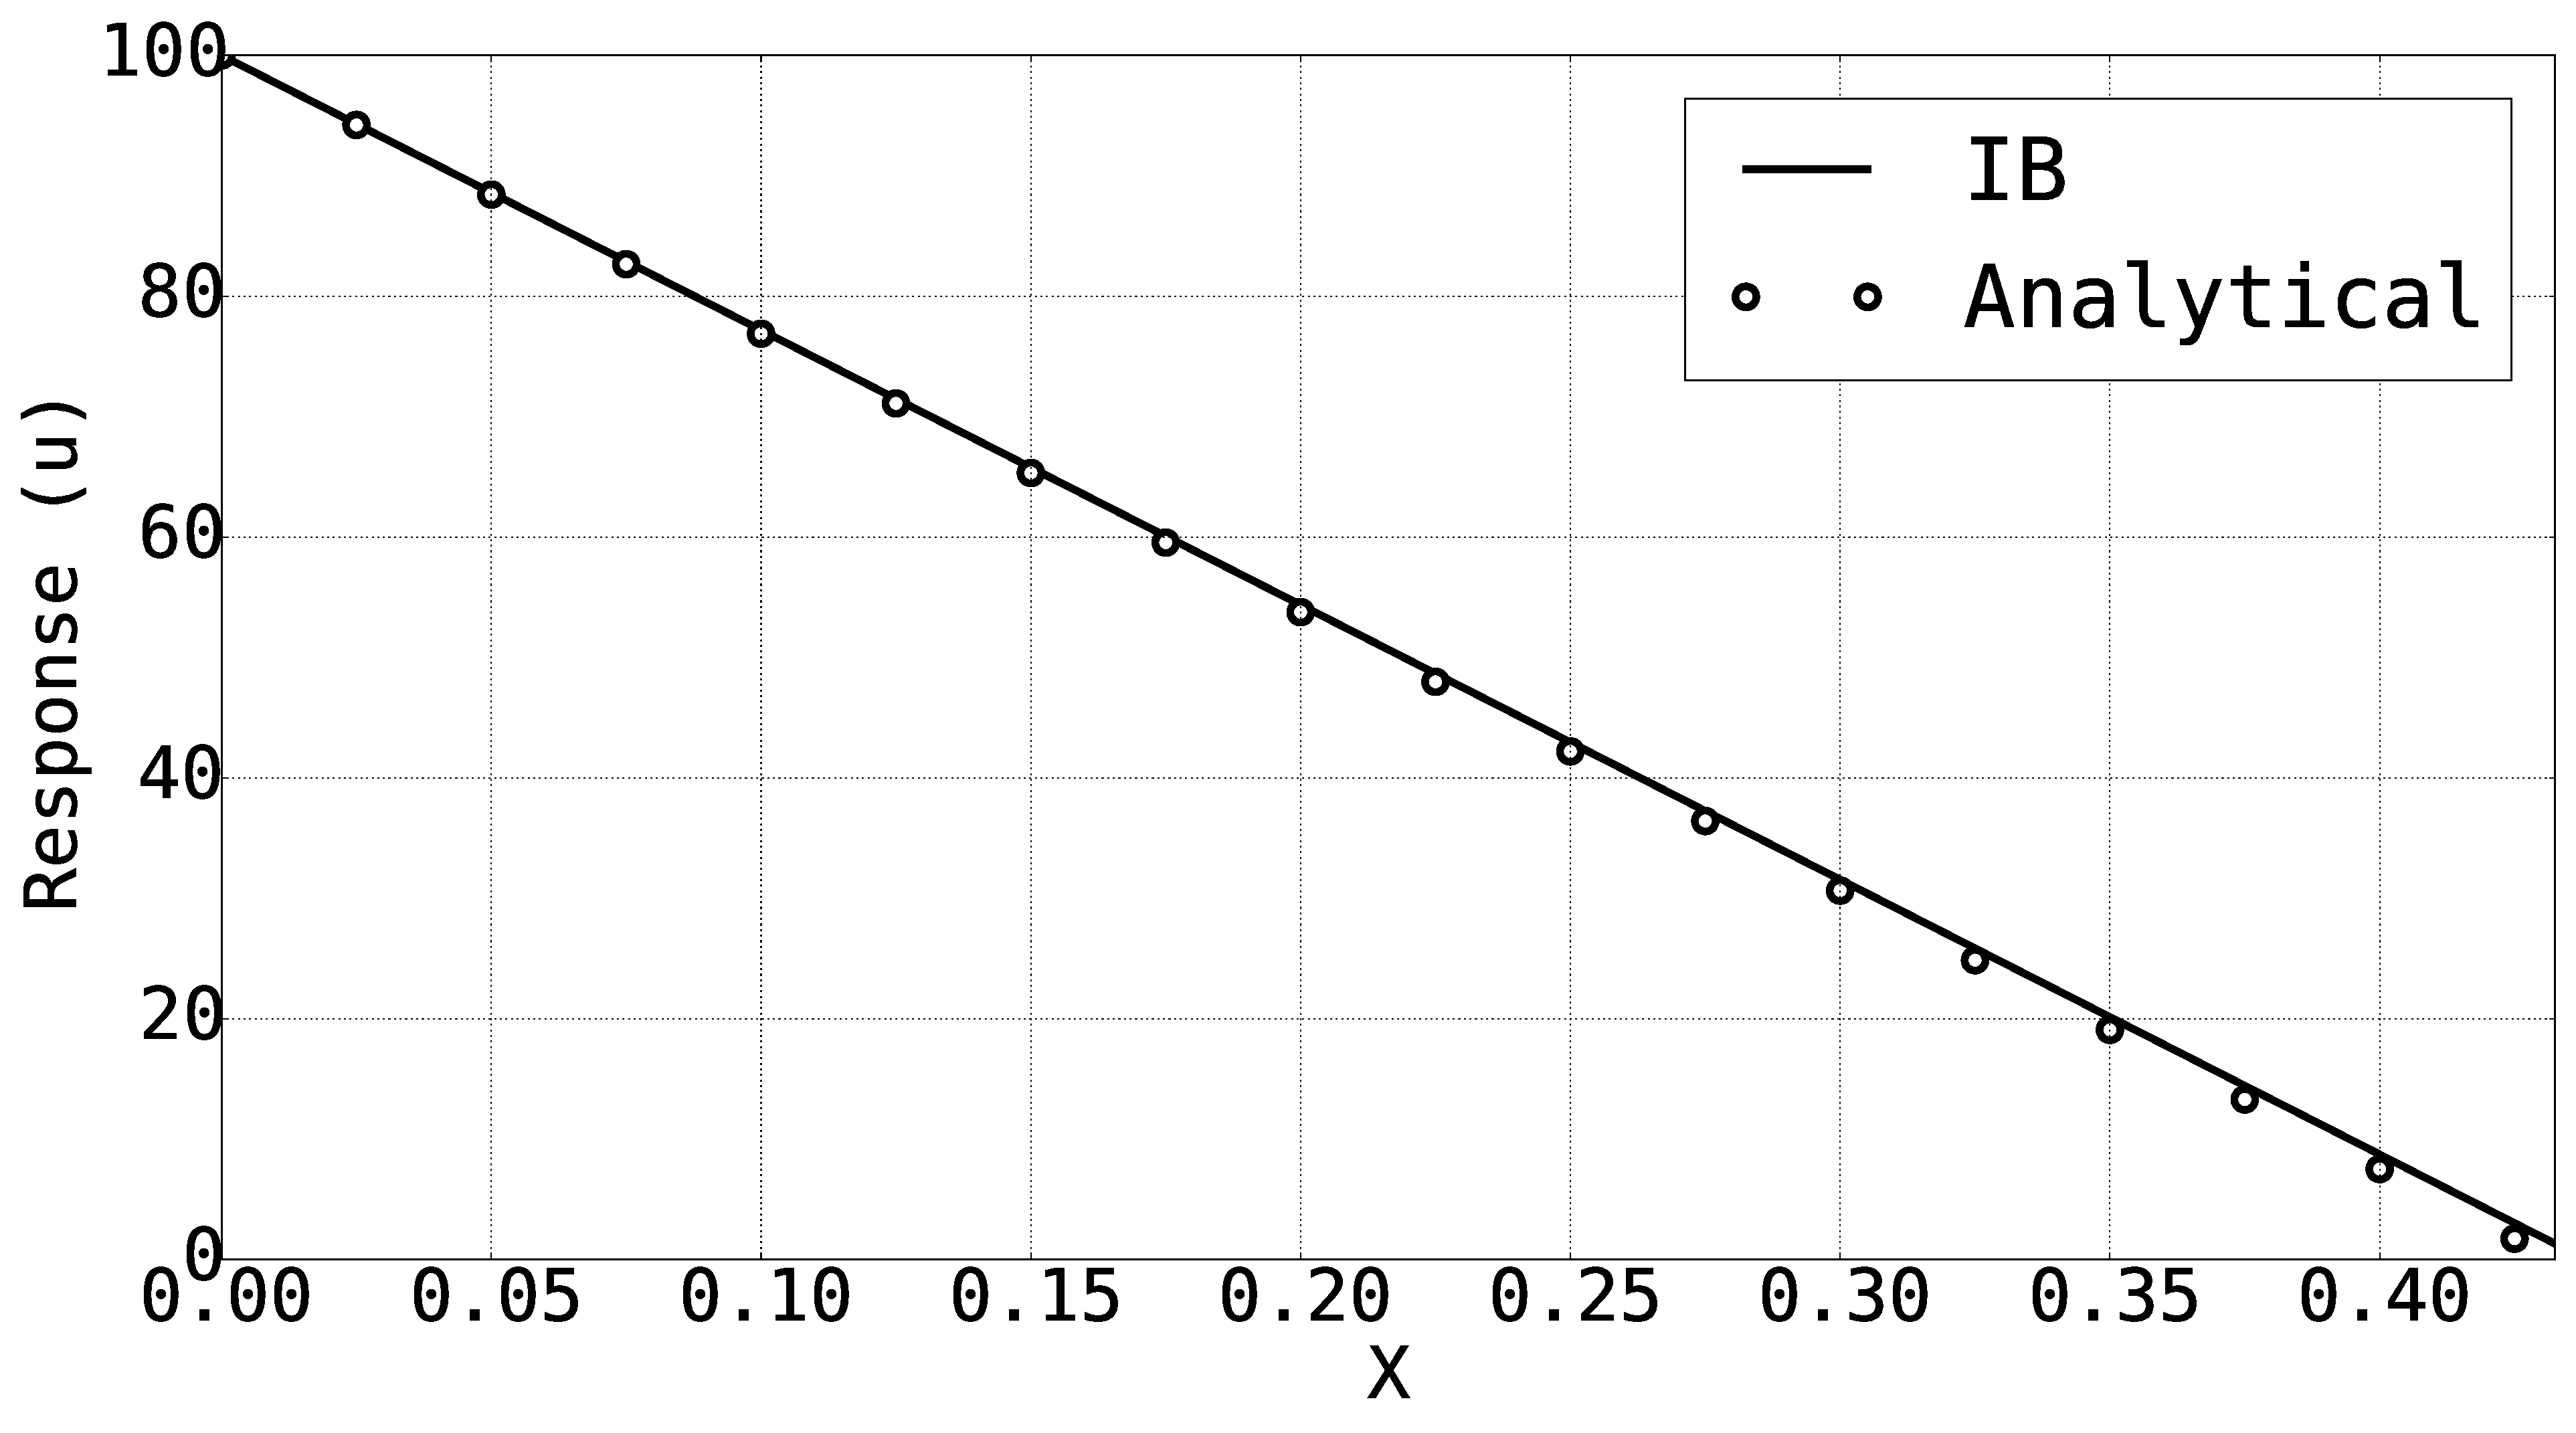
\includegraphics[width=7.0cm]{Chapter_3/figure/penalization_inletVelocity_100.eps}
	}
	\quad
	\subfigure[$U_{in} = 1000 m/s$]
	{
	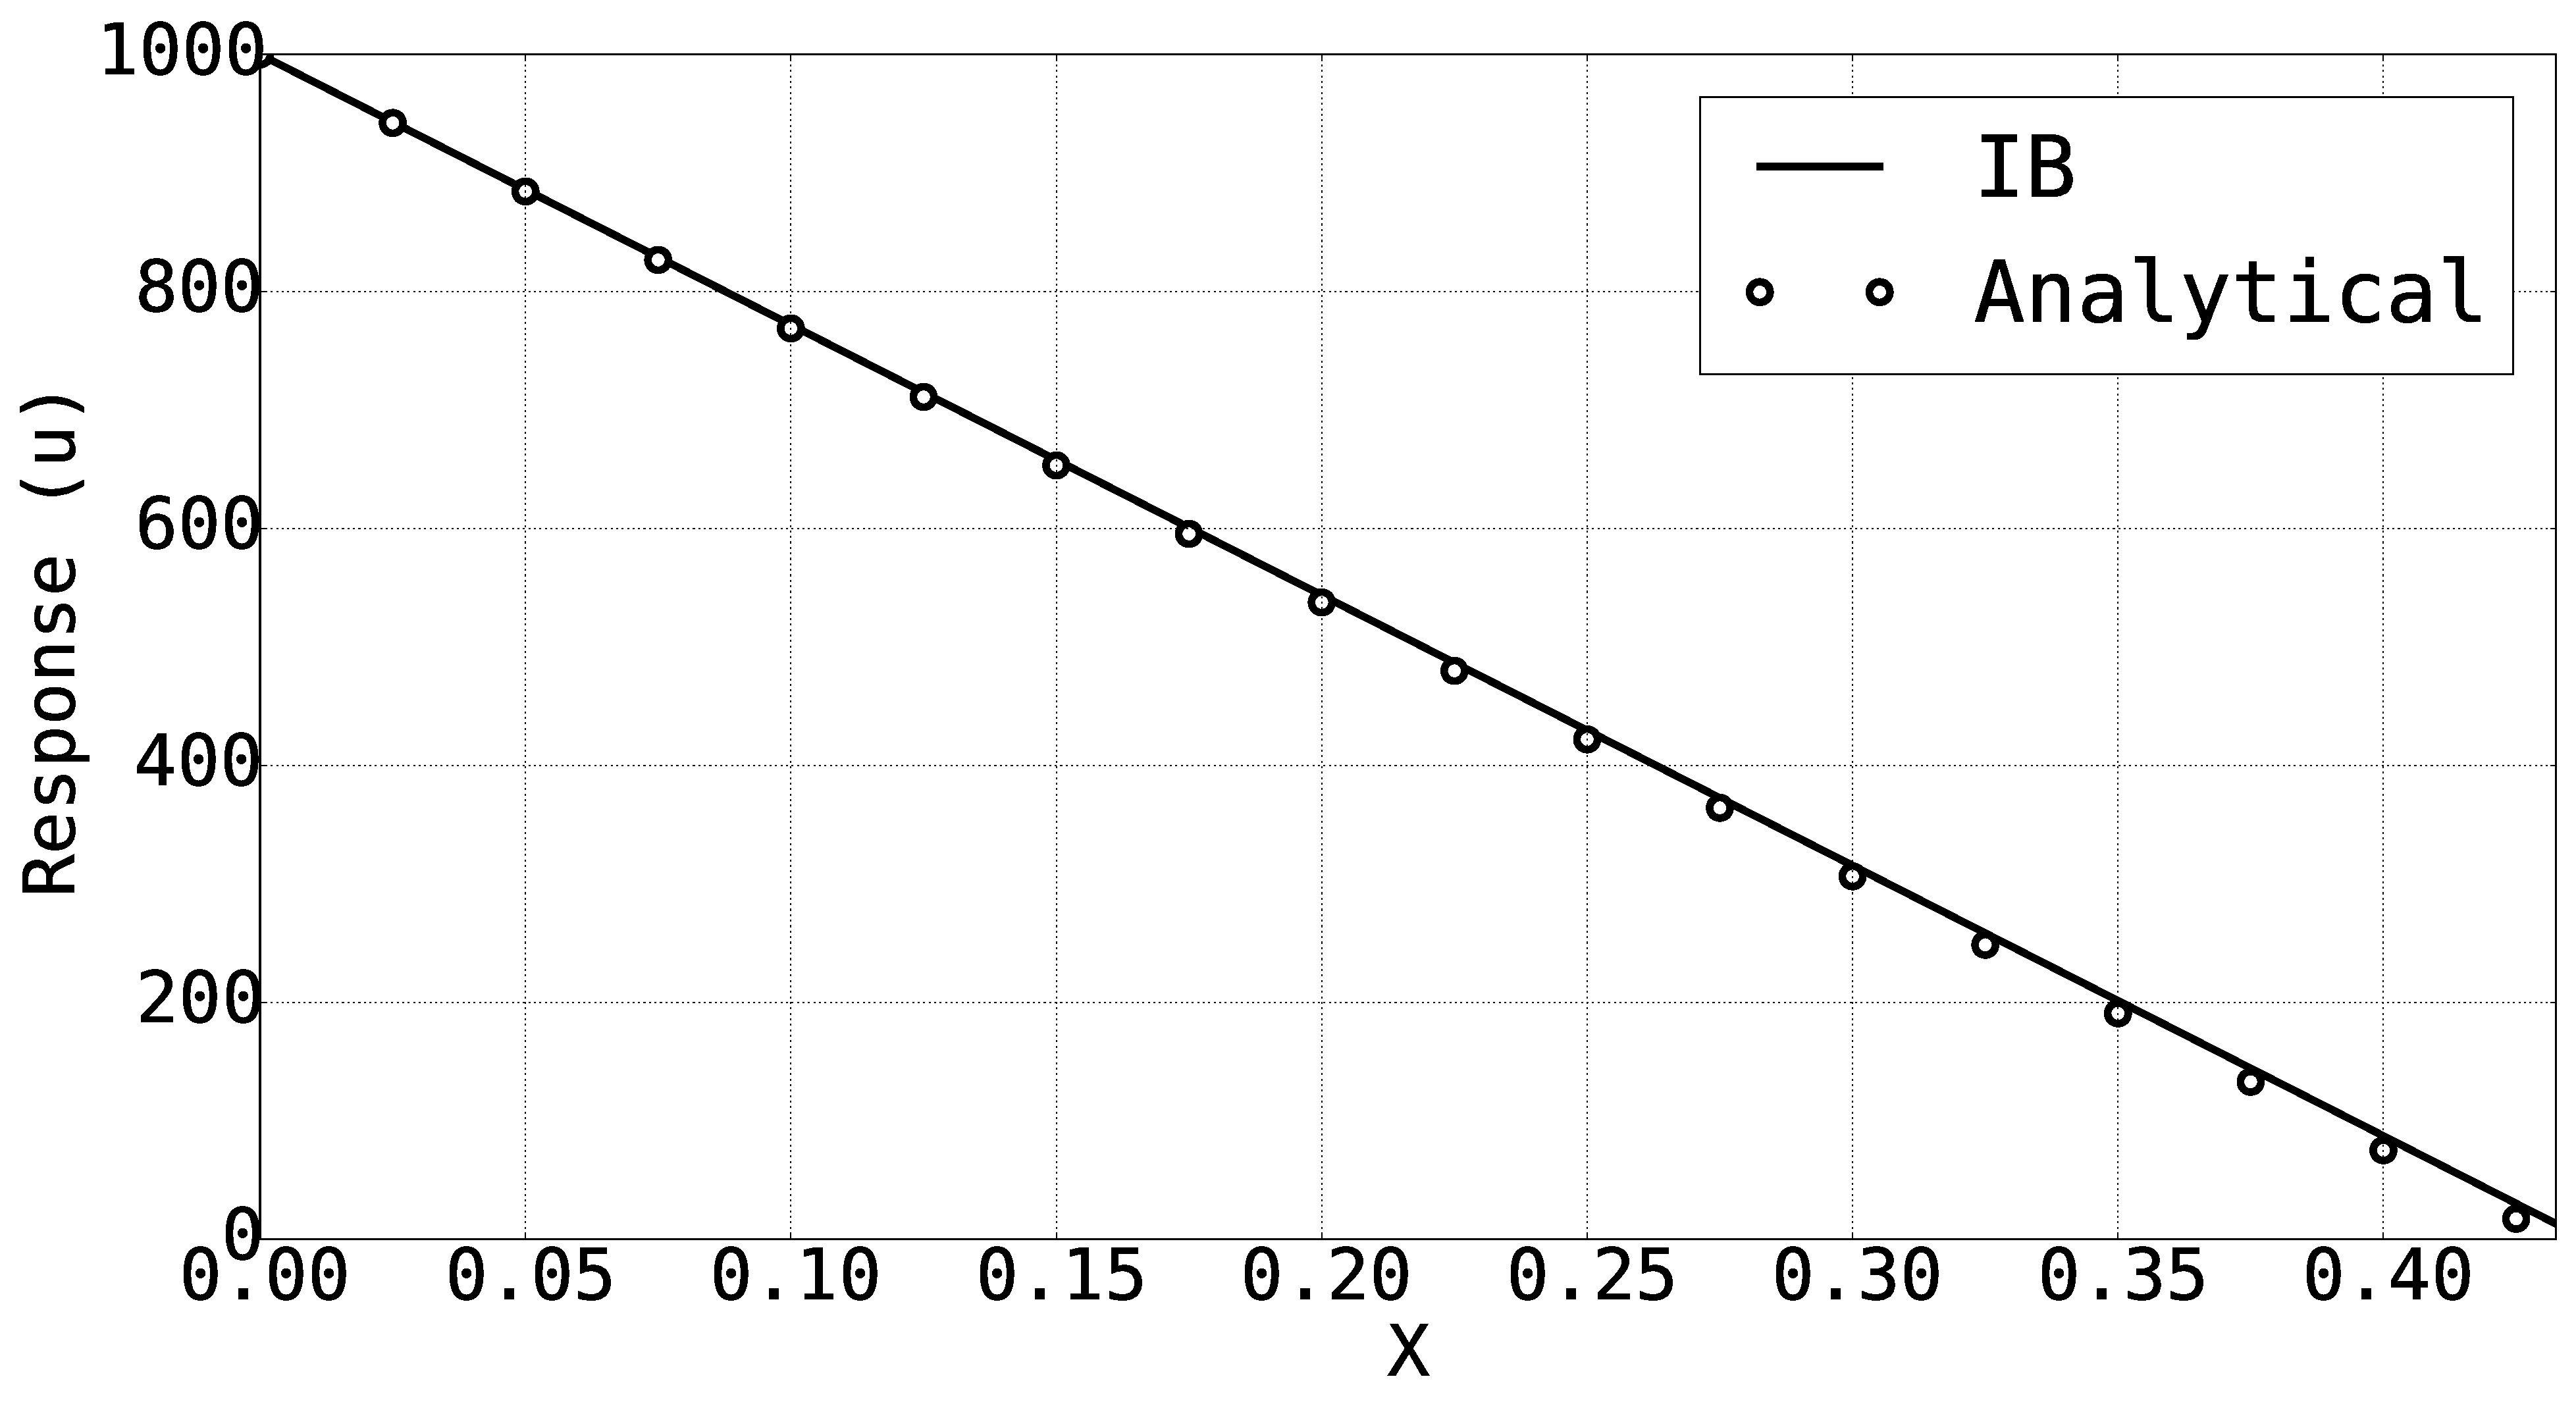
\includegraphics[width=7.0cm]{Chapter_3/figure/penalization_inletVelocity_1000.eps}
	}
	\caption{Comparison between IB and analytical results for different inlet velocity.}
	\label{fig:C3_penalizationResultInletVelocity}
\end{figure}

\begin{table}[H]
\centering
\begin{tabular}{c | c}
	Inlet velocity (m/s) & RMSE value \\ \hline \hline
	1 & 0.0056 \\ \hline
	10 & 0.0056 \\ \hline
	100 & 0.0056 \\ \hline
	1000 & 0.0056
\end{tabular}
\caption{RMSE value for different inlet velocities.}
\label{table:C3_penalizationResultInletVelocityRMSE}
\end{table}

Finally, we looked at the effect of different porosity values on the accuracy of the simulation. For this purpose, we fixed the wall location at $x_{wall} = 0.435$ and defined the velocity of the moving wall as $10 m/s$. The length of the domain is selected as $1 m$ and discretized using 81 nodes. We chose the time step as $10^{-5}$. We investigated the accuracy of penalization method to porosity values of $10^{-2}$, $10^{-3}$, $10^{-4}$, $10^{-5}$ by comparing the IB simulation with analytical results. The results shown in Figure \ref{fig:C3_penalizationResultPorosity} and Table \ref{table:C3_penalizationResultPorosityRMSE} shows the strong dependency of the simulation results of the porosity, $\kappa$, value. To select an appropriate porosity, several simulations need to be run and the convergence needs to be studied.

\begin{figure}[H]
	\centering
	\subfigure[$\kappa = 10^{-2}$]
	{
	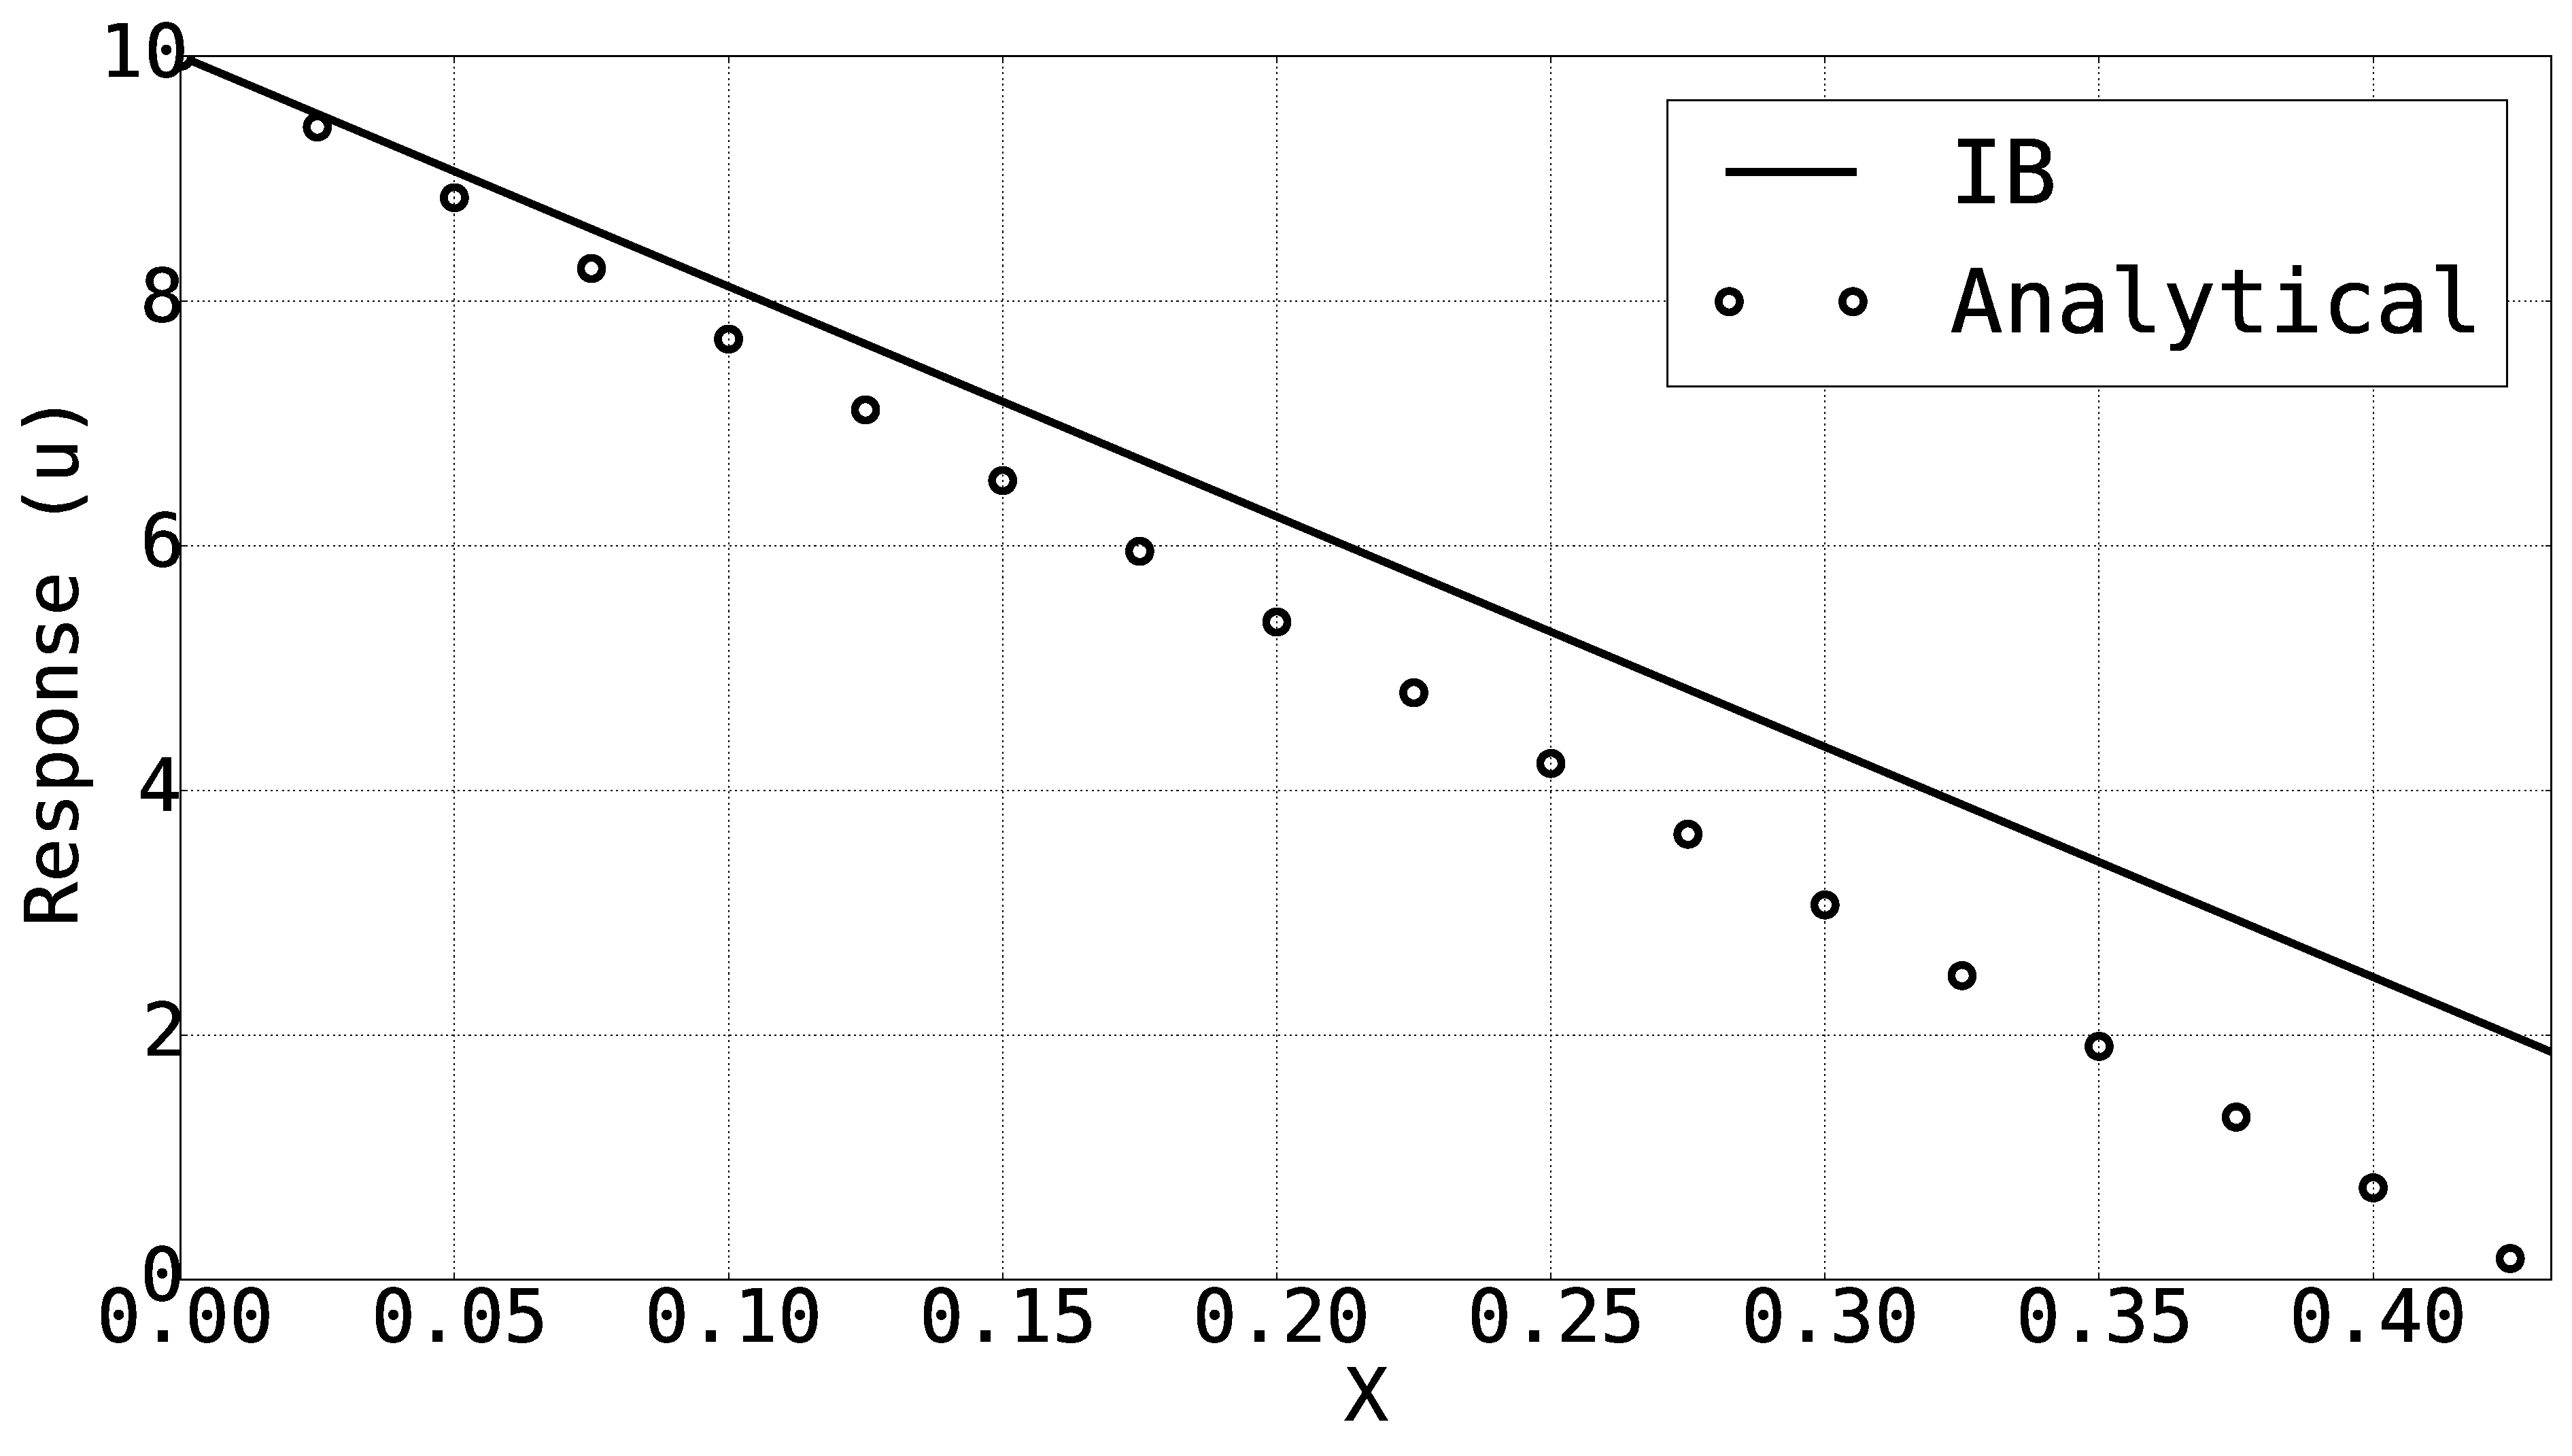
\includegraphics[width=7.0cm]{Chapter_3/figure/penalization_porosity_100.eps}
	}
	\quad
	\subfigure[$\kappa = 10^{-3}$]
	{
	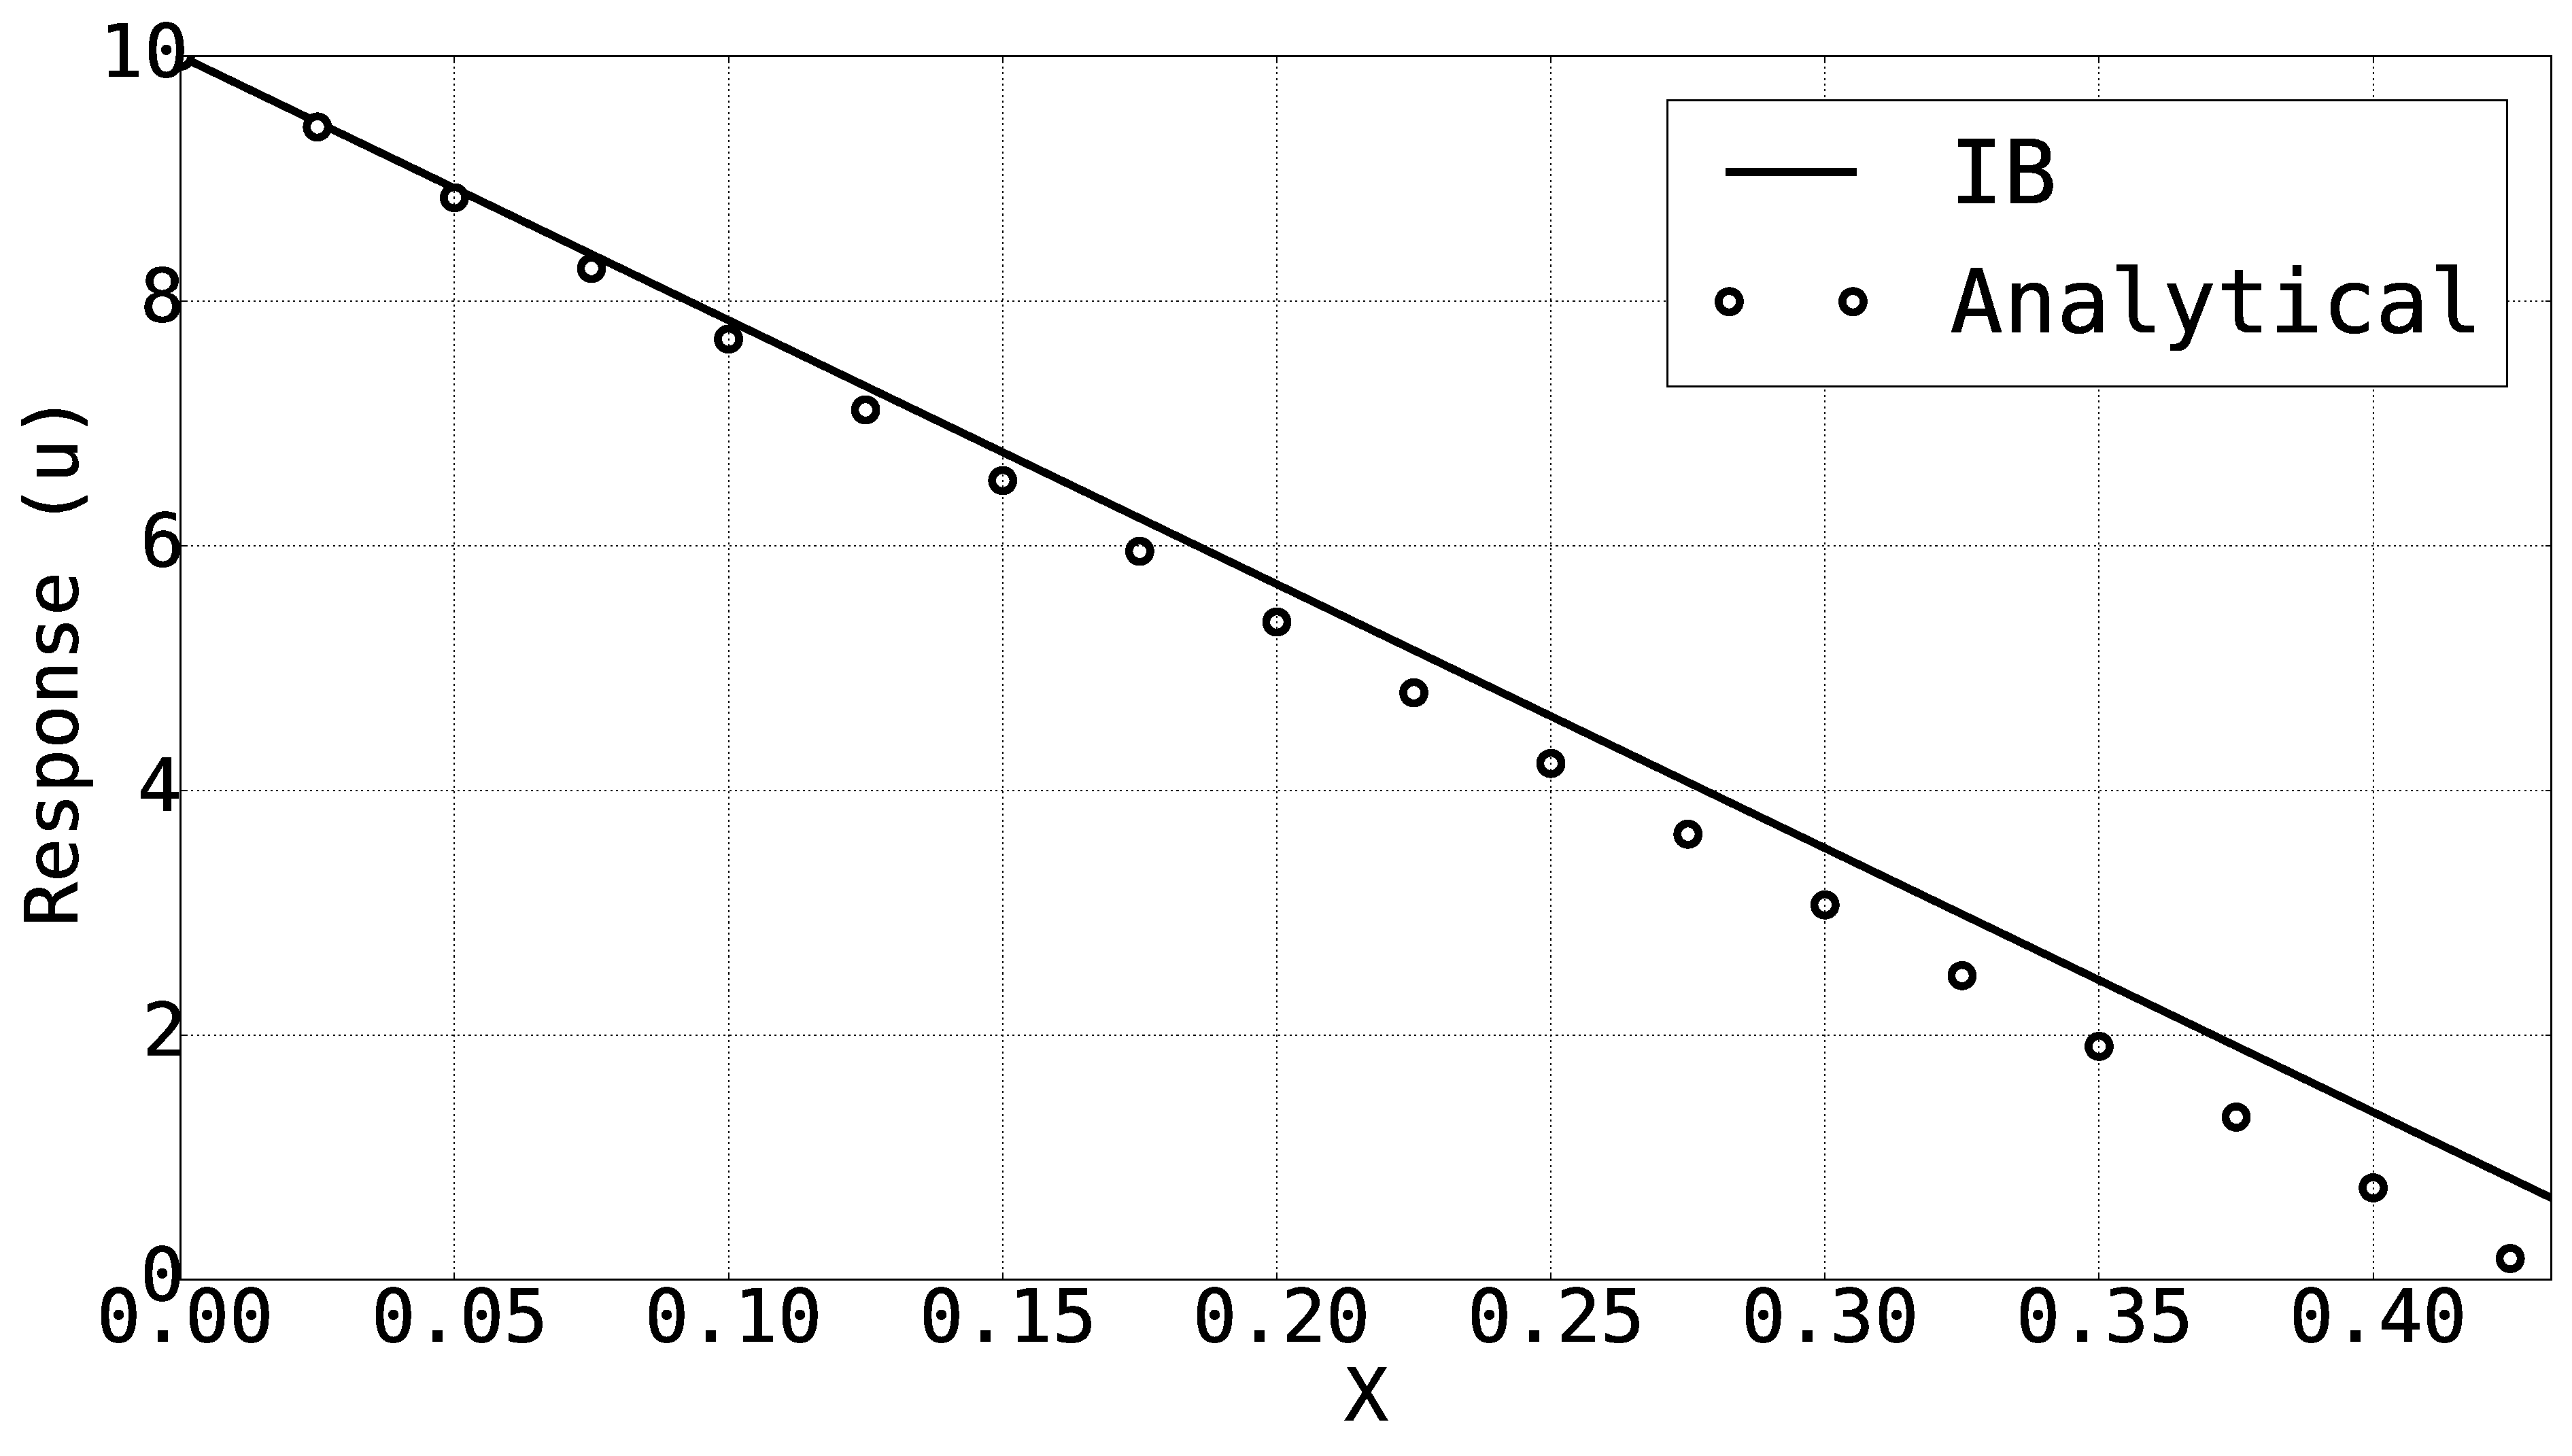
\includegraphics[width=7.0cm]{Chapter_3/figure/penalization_porosity_1000.eps}
	}
	\\
	\subfigure[$\kappa = 10^{-4}$]
	{
	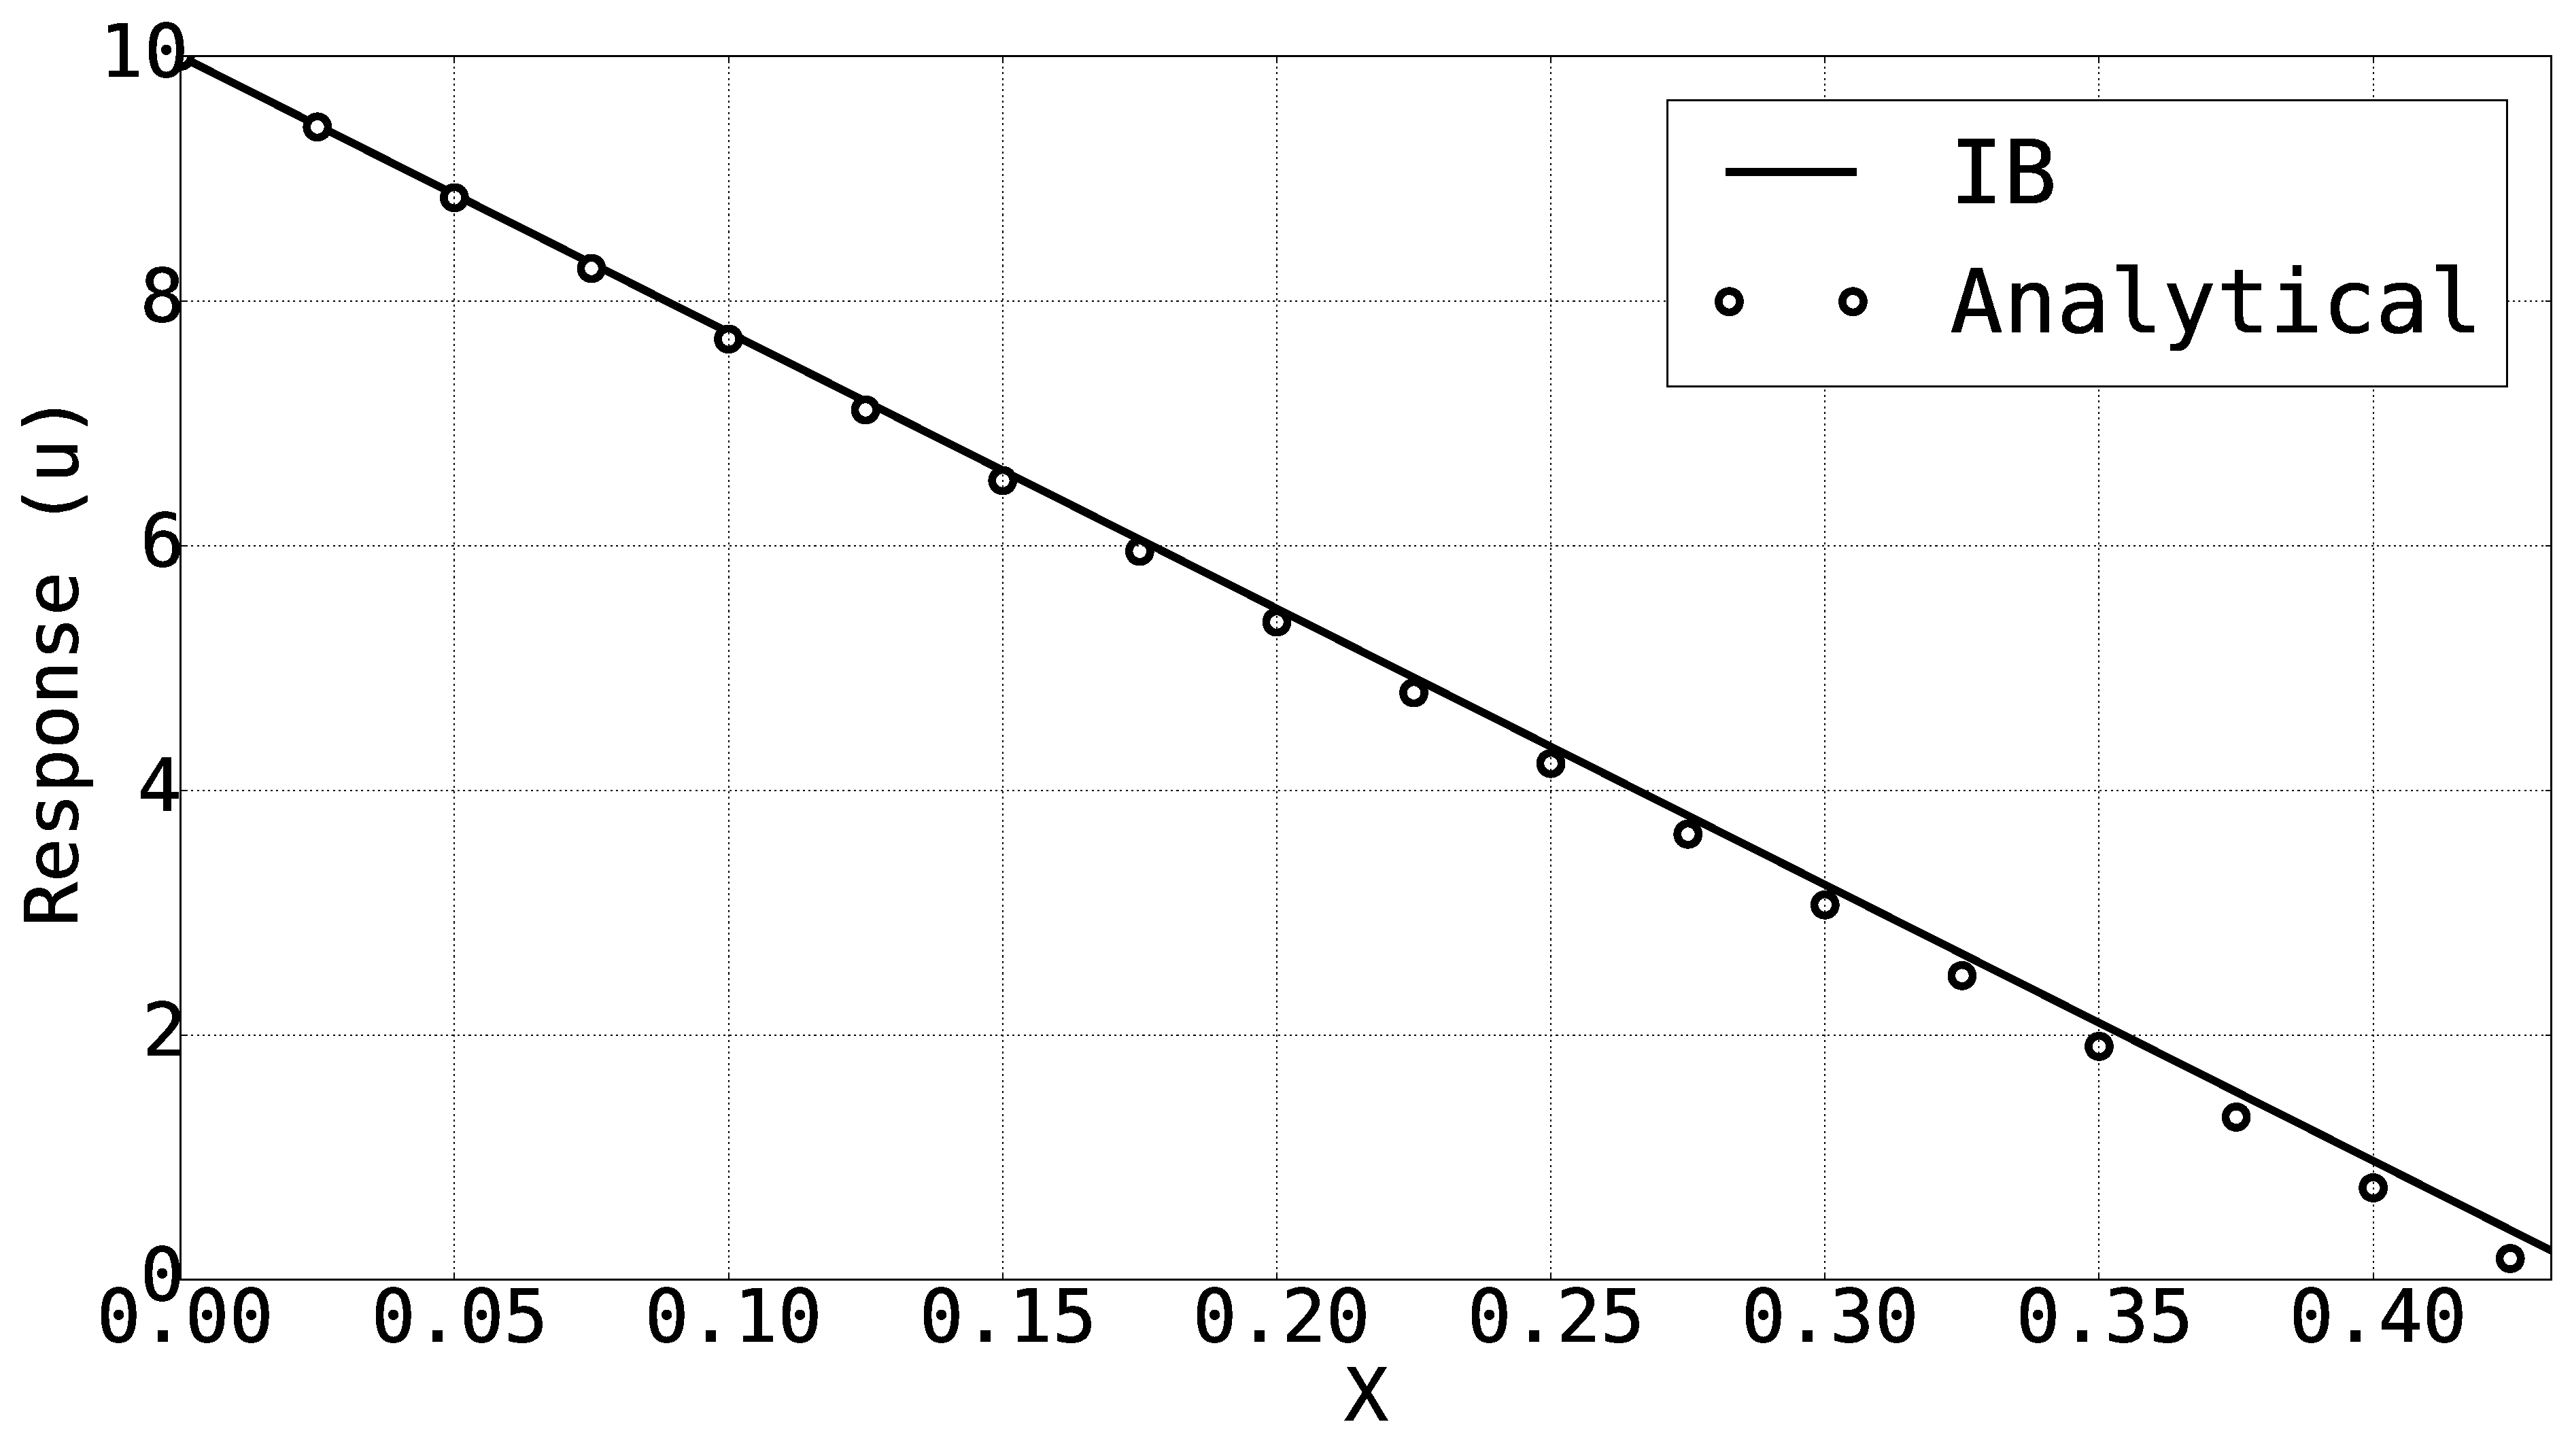
\includegraphics[width=7.0cm]{Chapter_3/figure/penalization_porosity_10000.eps}
	}
	\quad
	\subfigure[$\kappa = 10^{-5}$]
	{
	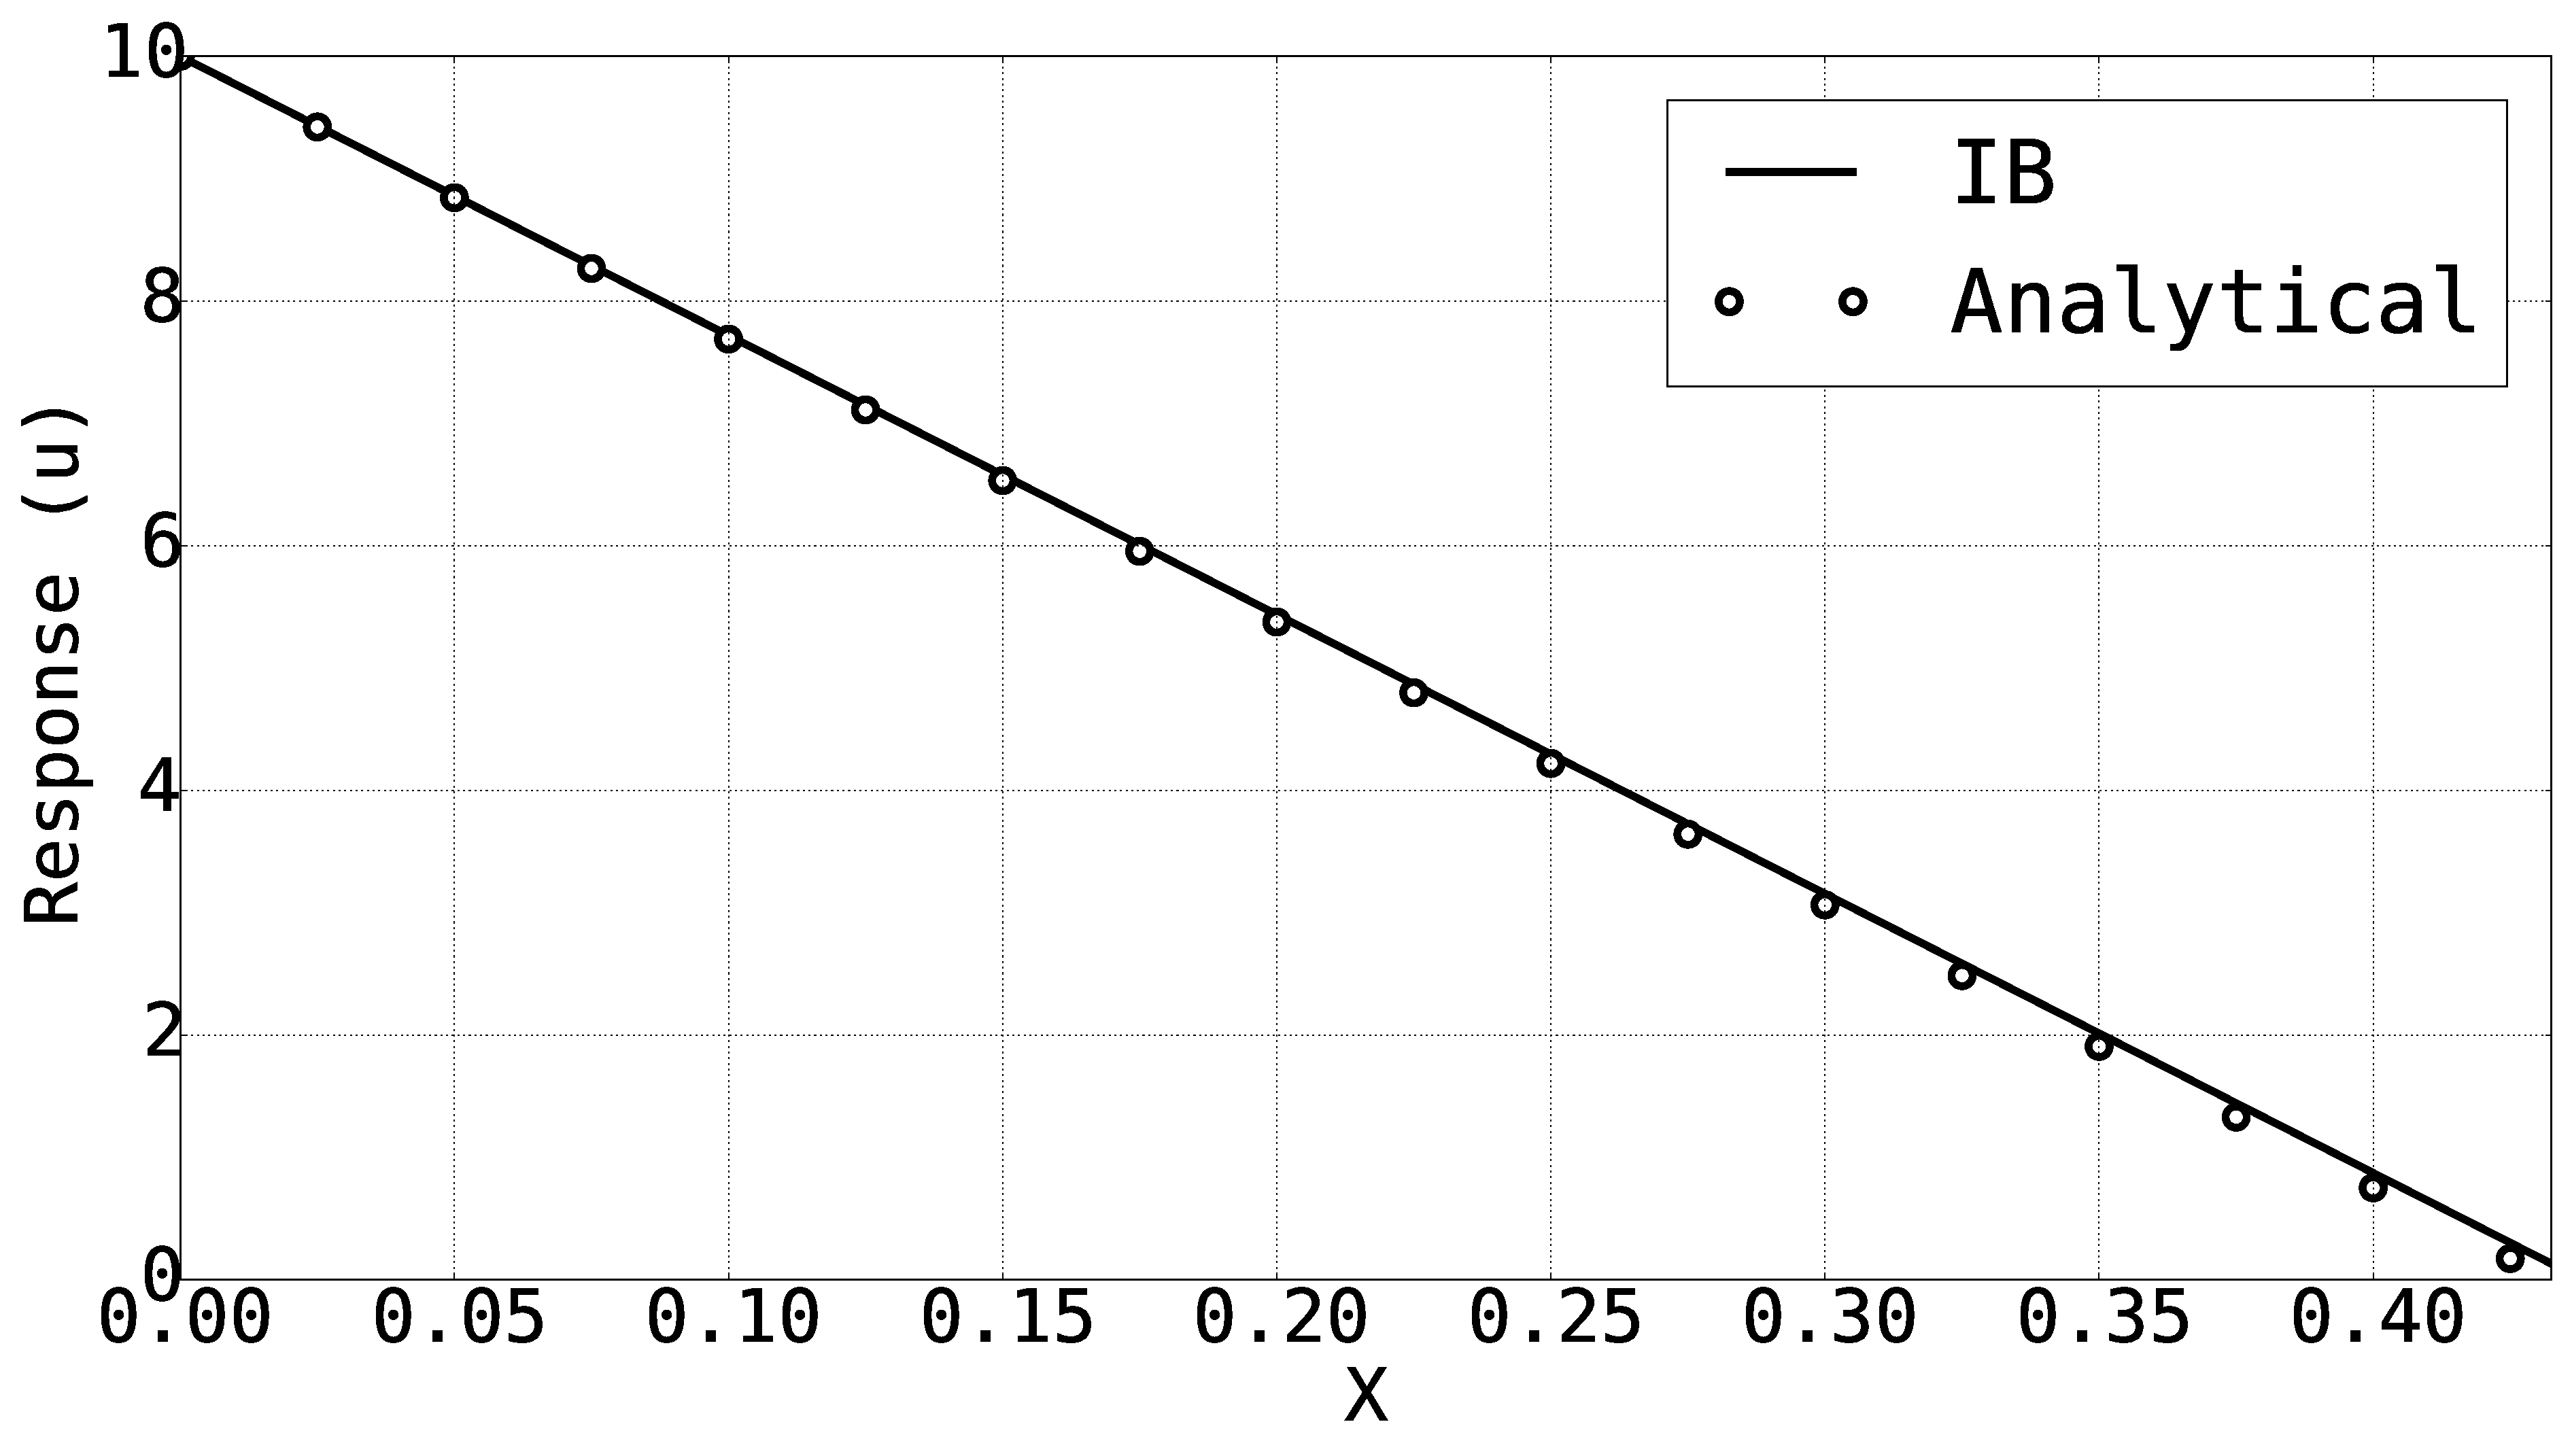
\includegraphics[width=7.0cm]{Chapter_3/figure/penalization_porosity_100000.eps}
	}
	\caption{Comparison between IB and analytical results for different porosity values.}
	\label{fig:C3_penalizationResultPorosity}
\end{figure}

\begin{table}[H]
\centering
\begin{tabular}{c | c}
	Porosity (m/s) & RMSE value \\ \hline \hline
	$10^{-2}$ & 0.079 \\ \hline
	$10^{-3}$ & 0.028 \\ \hline
	$10^{-4}$ & 0.01 \\ \hline
	$10^{-5}$ & 0.0056
\end{tabular}
\caption{RMSE value for different porosity values.}
\label{table:C3_penalizationResultPorosityRMSE}
\end{table}

The penalization method is probably the easiest one in the continuous IB methods to implement however, its accuracy is very dependent on the number of nodes used. This is because there are no mechanisms to exactly define the location of solid boundaries in the penalization method. This can lead to loss of accuracy and oscillations near the boundaries. The porosity value, $\kappa$, needs to be selected by running multiple simulations are compare the results for convergence. Although even with low values of porosities, there is a leakage in the solid domain that reduces the accuracy of the simulations.

%\subsubsection{Formulation}
%\subsubsection{Implimentation for Couette Flow Problem}
%\subsection{Cut-cell Method}
%\subsubsection{Formulation}
%\subsubsection{Implimentation for Couette Flow Problem}
%\section{Application in Continuum Sensitivity Analysis}
%\section{Summary}